\documentclass[spanish,UNC]{book}
%\documentclass[spanish,KINDLE]{book}
%\documentclass[spanish,12pt,openany]{book} % genera .pdf para kindle.
%\documentclass[spanish,11pt,AMAZON]{book} 
%\usepackage{babel,latexsym,html,graphics,pictex,epsfig}
\usepackage{color}
\usepackage{babel}
\usepackage{latexsym}
%\usepackage{graphics,pictex,epsfig}
\usepackage[latin1]{inputenc}
%\documentstyle{libro}
%\includeonly{chap11,chap13}
%\usepackage{garamond}
\usepackage[T1]{fontenc}
\usepackage{lmodern}

%%%%%%%%%%%%%%%%%%%%%%%%%%%%% PDFLaTeX  !!!!!!!!!!!!!!!!!!!!!!!!!!!!!!!!!! **********************
% From the PDFTeX FAQ:
% \newif\ifpdf
% \ifx\pdfoutput\undefined
%    \pdffalse           % not running PDFLaTeX
% \else
%    \pdfoutput=1
%    \pdftrue            % running PDFLaTeX
% \fi
% 
% \ifpdf
 %   \pdfcompresslevel=9
 %    \providecommand{\myinput}[1]{\input{#1.pdftex_t}}
 %   \usepackage[pdftex]{graphicx}
% \else
    \providecommand{\myinput}[1]{\input{#1.pstex_t}}
    \usepackage{graphicx}
% \fi


%\usepackage[T1]{fontenc}
\usepackage[urw-garamond]{mathdesign}

%\renewcommand{\rmdefault}{ugm}

\input format_libro

%\setcounter{chapter}{7}
%\setcounter{section}{4}
%\setcounter{subsection}{2}
%\setcounter{page}{82}
%\setcounter{equation}{88}
%\setcounter{part}{1}

\begin{document}%\dag
%\input{extdef}
%\typeout{**********************************************************}
%\typeout{***************** Loading PICHU's Macros *****************}
%\typeout{**********************************************************}


%\renewcommand{\@evenhead}{}
%\renewcommand{\@oddhead}{}
%\renewcommand{\@evenhead}{hfil\thepage\hfil}
%\renewcommand{\@oddhead}{\hfil\thepage\hfil}





\newcommand{\nc}{\newcommand}
\newcommand{\rnc}{\renewcommand}




%{\bf AQUI INGRESA EXTDEF}
%\message{acents, }

\def\ii{\'\i{}}
\def\a{\'a}
\def\e{\'e}
\def\o{\'o}
\def\u{\'u}

%\message{greek letters, }

\def\alf{\mbox{$\alpha$}}
\def\fit{\mbox{$\varphi (t)$}}
\def\fito{\mbox{$\varphi(t_0)$}}
\nc{\fip}{\mbox{$\varphi$}}
\def\fin{\mbox{$\varphi_n$}}
\nc{\fii}[1]{\mbox{$\varphi{#1}$}}
\def\gat{\mbox{ $\gamma (t)$}}
\def\gato{\mbox{ $\gamma(t_0)$}}
\def\gap{\mbox{ $\gamma$}}
\nc{\gay}[2]{\gamma_{#1}(#2)}
\def\lap{\mbox{$\lambda$}}
\def\lam{\mbox{$\lambda$}}
\def\eps{\mbox{$\varepsilon$}}
\def\del{\mbox{$\delta$}}
\nc{\tita}{\mbox{$\theta$}}
\nc{\ro}{\mbox{ $\rho$}}
\nc{\muu}{\mbox{ $\mu$}}
\nc{\Omeg}{\mbox{ $\Omega$}}
\nc{\tauu}{\mbox{ $\tau$}}
\nc{\psii}{\mbox{ $\psi$}}
\def\na{\nabla}
\def\Del{\Delta}

%\message{The "real" and ``complex'' symbol,}

\def\re{\mbox{\sl {l$\!\!\!\;\:\!$R}}}
\def\ren{\mbox{\sl {l$\!\!\!\;\:\!$R}$^n$}}
\def\Complex{C}

%\message{The napprox symbol,}

\newcommand{\napprox}{\mbox{ $\approx \!\!\!\!\! / $}}


%\message{utilities,}

\def\ti{\tilde}
\def\ifi{\infty}
\def\dip{\displaystyle}
\def\espa{\vskip \baselineskip}
\def\espc{\vskip 1in}
\nc{\hs}{\hspace{15mm}}
\nc{\noi}{\noindent}
\nc{\su}{\subset}
\nc{\ve}[1]{\mbox{\boldmath ${#1}$}}
\nc{\yaya}[1]{\underbar{#1}}

\rnc{\r}[1]{~\ref{#1}}
\nc{\ron}[1]{ (\ref{#1})}
\nc{\rtw}[2]{ (\ref{#1},\ref{#2})}
\nc{\rth}[3]{ (\ref{#1},\ref{#2},\ref{#3})}
\nc{\rfo}[4]{ (\ref{#1},\ref{#2},\ref{#3},\ref{#4})}



\nc{\beq}{\begin{equation}}
\nc{\eeq}{\end{equation}}
\nc{\barr}{\begin{array}}
\nc{\earr}{\end{array}}
\nc{\beqarr}{\begin{eqnarray}}
\nc{\eeqarr}{\end{eqnarray}}

\newtheorem{teo}{Teorema}[chapter]
\newtheorem{cor}{Corolario}[chapter]
\newtheorem{lem}{Lema}[chapter]
\newtheorem{pro}{Problema}[chapter]

\nc{\bteo}{\begin{teo}}
\nc{\eteo}{\end{teo}}
\nc{\bcor}{\begin{cor}}
\nc{\ecor}{\end{cor}}
\nc{\blem}{\begin{lem}}
\nc{\elem}{\end{lem}}
\nc{\ejem}{\espa \noi \underbar {Ejemplo}}
\nc{\ejer}{\espa\noi \underbar {Ejercicio}}
\nc{\pru}{\espa\noi \underbar {Prueba}}
\nc{\defi}{\espa\noi \underbar {Definici\'on}}
\nc{\epru}{$\;\;\spadesuit{}$}
\nc{\bpru}{\noi \underbar {Prueba}: }
\nc{\recu}[1]{\begin{center} \fbox{\parbox{11.cm}{\noi \small #1} }\end{center}}
\nc{\recubib}[1]{\begin{center} \vspace{0.5cm}\fbox{\parbox{11.cm}{{{\bf Notas bibliogr\'aficas:} {\noi \small #1}}}}\end{center}}
%\nc{\recubib}[1]{\vspace{1cm}\fbox{\parbox{15cm}{{{\bf Notas bibliogr\'aficas:} {\noi \small #1}}}}}
\nc{\bpro}{\begin{pro}}
\nc{\epro}{\end{pro}}
\nc{\Pro}{\noi \underbar {Problema}}
\nc{\ePro}{\vskip \baselineskip}

%\message{math definitions,}


\nc{\derp}[2]{\frac{\partial #1}{\partial #2}}
\nc{\dersp}[2]{\frac{\partial^2 #1}{\partial #2^2}}
\nc{\derssp}[3]{\frac{\partial^2 #1}{\partial #2 \partial #3}}
\nc{\derc}[2]{\frac{d #1}{d #2}}
\nc{\dersc}[2]{\frac{d^2 #1}{d #2^2}}
\nc{\der}[1]{\frac{d}{d #1}}
\nc{\lapl}[1]{\dersp{#1}{x}+\dersp{#1}{y}+\dersp{#1}{z}}
\nc{\pa}{\partial}

\nc{\nro}{$^{\mbox{o}}$}

\nc{\vA}{\mbox{$\ve A$}}
\nc{\vB}{\mbox{$\ve B$}}
\nc{\vL}{\mbox{$\ve L$}}

\nc{\xto}{\ve X_{t_0}^t}
\nc{\xot}{\ve X_t^{t_0}}
\nc{\xoti}{\ve X_{\tilde t}^{t_0}}
\nc{\x}{\mbox{$\ve X$}}
\nc{\cif}{\mbox{$C_0^{\ifi}(\re)$}}


%\message{more math utilities,}


\nc{\sr}[2]{\mbox{$\stackrel{#1}{#2}$}}
\nc{\fn}{\footnote}
\nc{\lme}{\lefteqn}
\nc{\nn}{\nonumber \\}
\nc{\fr}[2]{\mbox{$\frac{#1}{#2}$}}
\nc{\rpi}{\right|}
\nc{\lpi}{\left|}
\nc{\rp}{\right)}
\nc{\rdot}{\right.}
\nc{\ldot}{\left.}
\nc{\rb}{\right\}}
\nc{\lb}{\left\{}
\nc{\rc}{\right]}
\nc{\lc}{\left[}
\nc{\lp}{\left(}
\nc{\bb}{\bibitem}

\nc{\ex}{\mbox{$\exists$}}
\nc{\Ra}{\mbox{$\Rightarrow$}}
\nc{\Sii}{\mbox{$\Leftrightarrow$}}
\nc{\sii}{\mbox{$\leftrightarrow$}}
\nc{\fig}[2]{\begin{figure}\vspace{#1}\caption{#2}\end{figure}}
\nc{\mb}{\mbox}
\nc{\mt}{\mapsto}

\nc{\cL}{\mbox{$\cal L$}}
\nc{\cD}{\mbox{$\cal D$}}
\nc{\cP}{\mbox{$\cal P$}}
\nc{\cJ}{\mbox{$\cal J$}}
\nc{\scri}{\mbox{ {$\cal J$}}}
\nc{\cT}{\mbox{$\cal T$}}
\nc{\cC}{\mbox{$\cal C$}}
\nc{\cF}{\mbox{$\cal F$}}
\nc{\cS}{\mbox{$\cal S$}}


\nc{\LR}{\mbox{$L^2(\ren)$}}
\nc{\cifrn}{\mbox{$C^{\infty}(\ren)$}}
\nc{\cifo}{\mbox{$C^{\infty}_0$}}

%%% Local Variables: 
%%% mode: latex
%%% TeX-master: "apu_tot"
%%% End: 


%\garamond

%
\thispagestyle{empty}
\phantom{X}
\newpage
\thispagestyle{empty}
\phantom{X}
\newpage
\thispagestyle{empty}
\phantom{X}
\newpage
\thispagestyle{empty}
\phantom{X}
\newpage
%\thispagestyle{empty}
\phantom{X}
\vspace{5cm}
\begin{center}
 \textbf{\huge M\'etodos Matem\'aticos  de la F\'{\i}sica} \\
\vspace{1cm}
 \textbf{\Large \sc Oscar Reula}
\end{center}

\vspace{8cm}
\vfill

%\title{M\'etodos Matem\'aticos \\ de la F\'{\i}sica}

%\author{Oscar Reula %\thanks{Facultad de Matem\'aticas, Astronom\'{\i}a y F\'\i{}sica, Univ. Nac. C\'ordoba y CONICET}}

%\date{\sc{Diciembre} 2008}



% \begin{figure}[htbp]
%   \begin{center}
%     \resizebox{7cm}{!}{
\hspace{2.8cm} 
\begin{picture}(0,0)%
 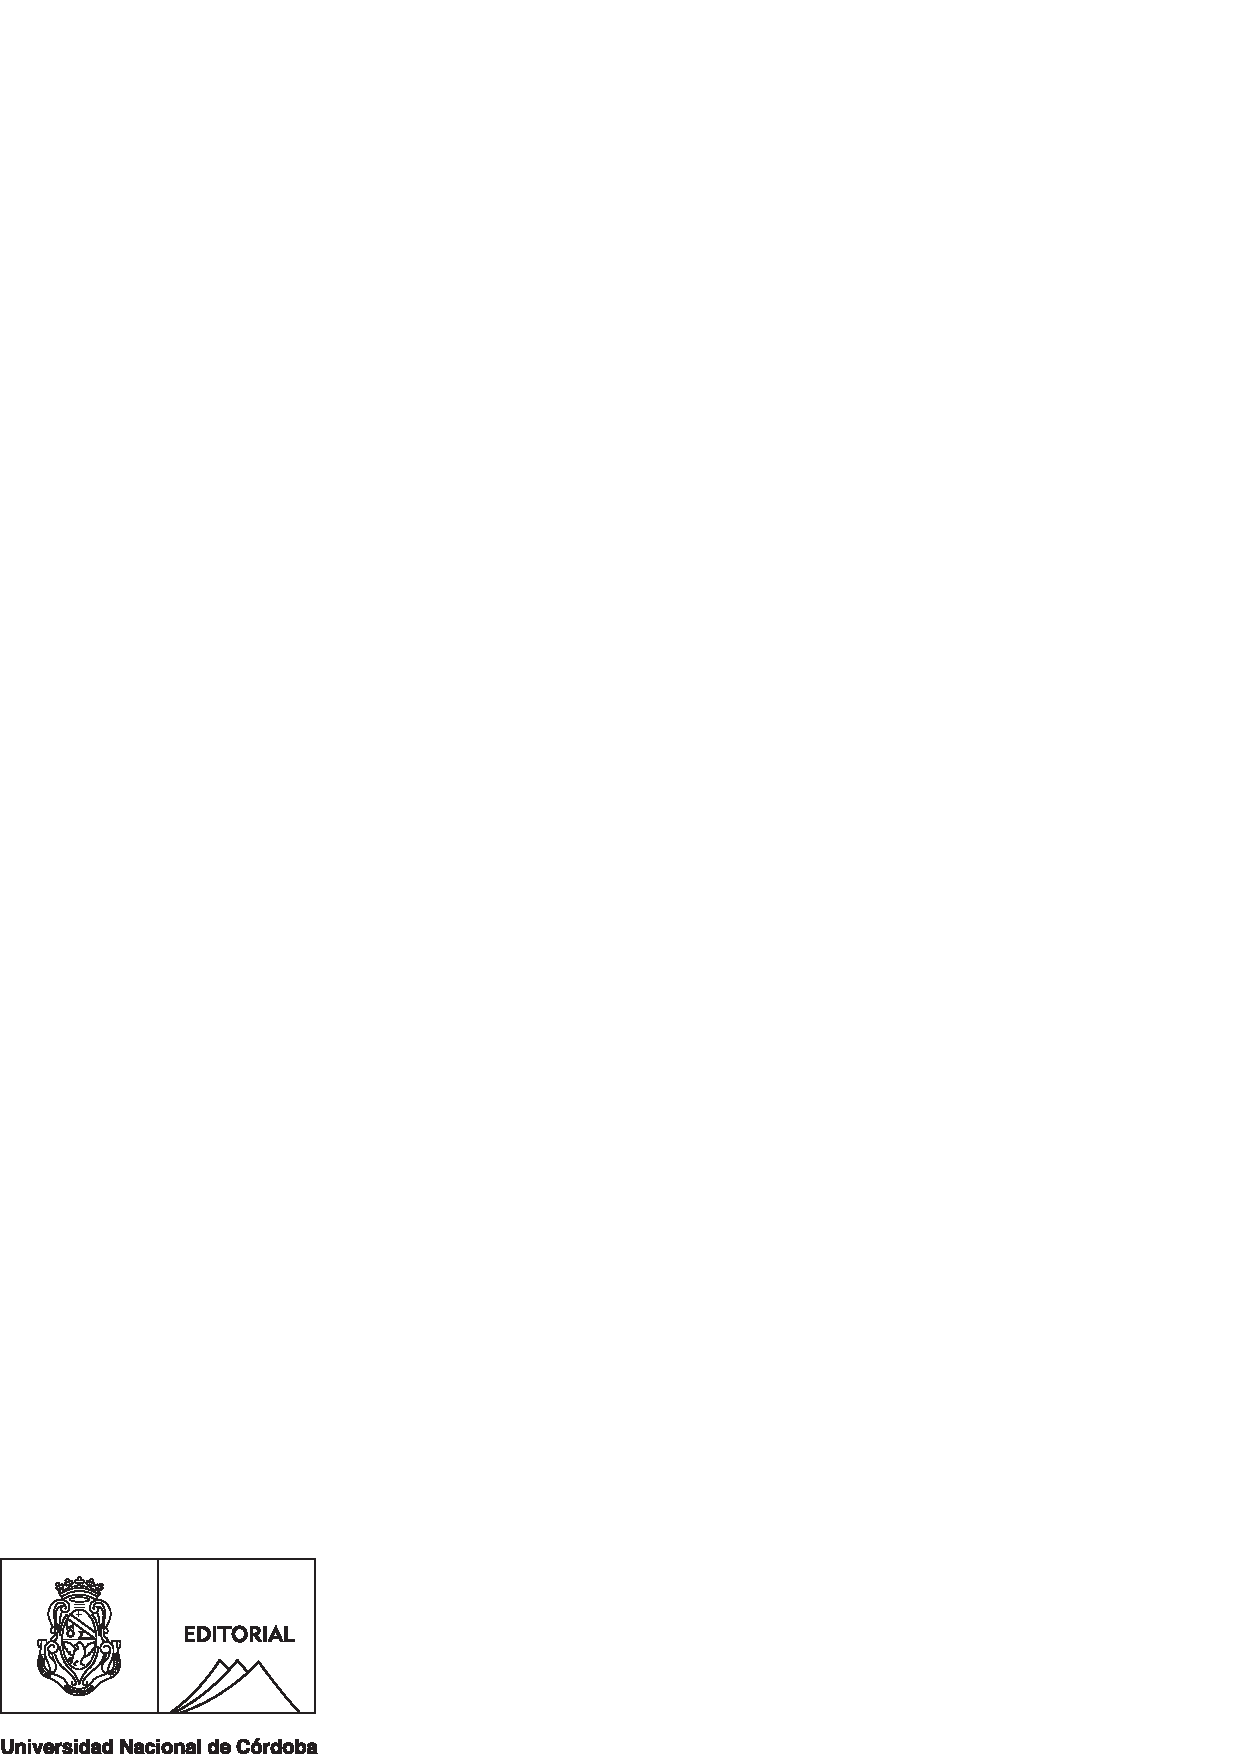
\includegraphics{Figure/logo.pdf}%
 \end{picture}
% }
    %\caption{Diagrama del operador dual.}
    %\label{fig:2_1}
%   \end{center}
% \end{figure}

%\maketitle

\phantom{X}%\dag
\vspace*{4cm}
\begin{center}
 \textbf{\huge M\'etodos Matem\'aticos  de la F\'{\i}sica} \\
\vspace{1cm}
 \textbf{\Large \sc Oscar Reula}
\end{center}
\vfill
\vspace*{5cm}
\phantom{Y}
\vfill



%\part{}

%%ultima modificación 13-08-92

%\input format


\chapter*{Agradecimientos}

En primer lugar quiero agradecer a Gloria Puente, por haberme apoyado durante todo el tiempo en que escribí estas notas, las cuales tomaron bastante tiempo de nuestras horas compartidas, en general largas noches.
En segundo lugar a Bernardo González Kriegel quien volcara a \LaTeX  las primeras versiones de estas notas, haciendo un gran trabajo con mucho entusiasmo. 
También a Bob Geroch, con quien discutí varios temas de las notas y de quien 
también me inspiré a través de sus escritos y libros, no solo en contenido sino también en estilo.
Finalmente a varias camadas de estudiantes que asimilaron estoicamente una gran cantidad del material de estos cursos en un tiempo demasiado corto.
% 
% 
% \chapter*{Prefacio:}
% 
% Estas notas, ahora devenidas en libro, se originaron como un intento de condensar en un
% solo lugar un gran conjunto de ideas, conceptos y herramientas matemáticas que considero básicas
% para la comprensión y el trabajo diario de un físico en nuestros días.
% 
% Usualmente sucede que si un problema es formulado desde una necesidad de origen físico, como por ejemplo la descripción de algún 
% fenómeno  natural, entonces éste esta bien formulado, en el sentido de que una solución razonable al mismo existe.
% Esta regla ha sido en general muy fructífera y en particular les ha servido como guía a muchos matemáticos
% para abrirse camino en áreas desconocidas. Pero también ha servido, en particular a muchos físicos, para 
% trabajar sin preocuparse demasiado por aspectos formales, ya sean analíticos, algebraicos o geométricos 
% y poder así concentrarse en aspectos físicos y/o computacionales. 
% Si bien esto permite un rápido desarrollo de algunas investigaciones, a la larga se llega a un estancamiento
% pues al proceder de este modo se evita enfrentar problemas que son muy ricos en cuanto a la conceptualización
% del fenómeno a describir. Es importante constatar que el problema formulado tiene una solución matemática y físicamente
% correcta.
% 
% Un ejemplo de esto ha sido el desarrollo, a mediados del siglo pasado, de la teoría
% moderna de las ecuaciones en derivadas parciales. Muchas de estas ecuaciones surgieron debido a que describen 
% fenómenos de físicos: transmisión del calor, propagación de ondas electromagnéticas, ondas cuánticas, gravitación, etc.
% Una de las primeras respuestas matemáticas al desarrollo de estas áreas fue el teorema de Cauchy-Kowalevski que nos dice que dada una ecuación 
% en derivadas parciales, (bajo ciertas circunstancias bastante generales)
% si una función analítica es dada como dato en una hipersuperficie (con ciertas características), luego existe una solución 
% única en un entorno suficientemente pequeño de dicha hipersuperficie. Tomó mucho tiempo darse cuenta que este teorema realmente
% no era relevante desde el punto de vista de las aplicaciones físicas: existían ecuaciones admitidas por el teorema tales que si
% el dato no era analítico ¡no había solución! Y en muchos casos, si éstas existían, no dependían continuamente del dato dado,
% una pequeña variación del dato producía una solución totalmente distinta. Recién a mediados del siglo pasado se logró un
% avance sustancial al problema, encontrando que habían distinto tipo de ecuaciones, hiperbólicas, elípticas, parabólicas, etc.
% que se comportaban de manera distinta y esto reflejaba los distintos procesos físicos que las mismas simulaban.
% Debido a su relativa actualidad, este conjunto tan importante de conceptos no forman parte del conjunto de herramientas con que
% cuentan muchos de los físicos en actividad ni tampoco se encuentran en los libros de texto usualmente utilizados en las carreras de grado.
% 
% Como el anterior hay muchos ejemplos, en particular la teoría de ecuaciones diferenciales ordinarias y la geometría, sin la cual es imposible
% comprender muchas de las teorías modernas, tales como la relatividad, las teorías de partículas elementales y muchos fenómenos
% de la física del estado sólido.
% A medida que avanza nuestra comprensión de los fenómenos básicos de la naturaleza más nos damos cuenta que la herramienta más importante
% para su descripción es la geometría. Esta, entre otras cosas, nos permite manejar una amplia gama de procesos y teorías sin mucho en común entre sí con un conjunto muy reducido de conceptos, lográndose así una síntesis. Éstas síntesis son las que nos permiten adquirir nuevos conocimientos,
% ya que mediante su adopción dejamos espacio en nuestras mentes para aprender nuevos conceptos, los cuales son a su vez ordenados de manera más eficiente
% dentro de nuestra construcción mental del área.
% 
% Estas notas fueron originalmente pensadas para un curso de cuatro meses de duración. Pero en realidad se adaptaban más para un curso anual o dos
% semestrales. Luego, a medida que se fueron incorporando más temas a las mismas, resultó más y más claro que deben darse en dos cursos semestrales o
% uno anual. 
% Básicamente un curso debería contener los primeros capítulos que incluyen nociones de topología, espacios vectoriales, álgebra lineal,
% finalizando con la teoría de las ecuaciones en derivadas ordinarias. La tarea se simplifica considerablemente si los estudiantes han tenido previamente un buen curso de álgebra lineal. La correlación con las materias de física debería ser tal que el curso sea previo o concurrente con una mecánica avanzada.
% Haciendo hincapié en la misma sobre el hecho de que en definitiva uno está resolviendo ecuaciones diferenciales ordinarias con cierta estructura especial.
% Utilizando los conceptos del álgebra lineal para encontrar modos propios y la estabilidad de puntos de equilibrio. Y finalmente utilizando la geometría para
% describir aunque más no sea someramente la estructura simpléctica subyacente.
% 
% El segundo curso consiste en desarrollar las herramientas para poder discutir aspectos de la teoría de ecuaciones en derivadas parciales.
% Debería darse antes o concurrentemente con un curso avanzado de electromagnetismo, donde se debería hacer hincapié en el tipo de ecuaciones
% que se resuelven (elípticas, hiperbólicas), y el sentido de sus condiciones iniciales o de contorno, según corresponda. Usando además en forma
% coherente el concepto de distribución, que lejos de ser un concepto matemático abstracto es en realidad un concepto que aparece naturalmente en la física.
%  
% Nada del contenido de estas notas es material original, sí algunas formas de presentarlo, por ejemplo algunas pruebas más simples que las usuales, o la forma de integrar cada contenido con los anteriores. Mucho del material debería ser pensado como una primera lectura o una iniciación al tema y el lector interesado en profundizar debería leer los libros citados, de los cuales he extraído mucho material, siendo éstos excelentes y difíciles de superar.
% 
% 
% 
% 


\tableofcontents
\listoffigures
T
%\garamond



\chapter*{Prefacio}

Estas notas, ahora devenidas en libro, se originaron como un intento de condensar en un
solo lugar un gran conjunto de ideas, conceptos y herramientas matem�ticas que considero b�sicas
para la comprensi�n y el trabajo diario de un f�sico en nuestros d�as.

Usualmente sucede que si un problema es formulado desde una necesidad de origen f�sico, como por ejemplo la descripci�n de alg�n 
fen�meno  natural, entonces �ste est� bien formulado, en el sentido de que una soluci�n razonable al mismo existe.
Esta regla ha sido en general muy fruct�fera y en particular les ha servido como gu�a a muchos matem�ticos
para abrirse camino en �reas desconocidas. Pero tambi�n ha servido, en particular a muchos f�sicos, para 
trabajar sin preocuparse demasiado por aspectos formales, ya sean anal�ticos, algebraicos o geom�tricos 
y poder as� concentrarse en aspectos f�sicos y/o computacionales. 
Si bien esto permite un r�pido desarrollo de algunas investigaciones, a la larga se llega a un estancamiento
pues al proceder de este modo se evita enfrentar problemas que son muy ricos en cuanto a la conceptualizaci�n
del fen�meno a describir. Es importante constatar que el problema formulado tiene una soluci�n matem�tica y f�sicamente
correcta.

Un ejemplo de esto ha sido el desarrollo, a mediados del siglo pasado, de la teor�a
moderna de las ecuaciones en derivadas parciales. Muchas de estas ecuaciones surgieron debido a que describen 
fen�menos de f�sicos: transmisi�n del calor, propagaci�n de ondas electromagn�ticas, ondas cu�nticas, gravitaci�n, etc.
Una de las primeras respuestas matem�ticas al desarrollo de estas �reas fue el teorema de Cauchy-Kowalevski que nos dice que dada una ecuaci�n 
en derivadas parciales, (bajo ciertas circunstancias bastante generales)
si una funci�n anal�tica es dada como dato en una hipersuperficie (con ciertas caracter�sticas), luego existe una soluci�n 
�nica en un entorno suficientemente peque�o de dicha hipersuperficie. Tom� mucho tiempo darse cuenta que este teorema realmente
no era relevante desde el punto de vista de las aplicaciones f�sicas: exist�an ecuaciones admitidas por el teorema tales que si
el dato no era anal�tico �no hab�a soluci�n! Y en muchos casos, si �stas exist�an, no depend�an continuamente del dato dado,
una peque�a variaci�n del dato produc�a una soluci�n totalmente distinta. Reci�n a mediados del siglo pasado se logr� un
avance sustancial al problema, encontrando que hab�an distintos tipos de ecuaciones, hiperb�licas, el�pticas, parab�licas, etc.
que se comportaban de manera distinta y esto reflejaba los distintos procesos f�sicos que las mismas simulaban.
Debido a su relativa actualidad, este conjunto tan importante de conceptos no forman parte del conjunto de herramientas con que
cuentan muchos de los f�sicos en actividad ni tampoco se encuentran en los libros de texto usualmente utilizados en las carreras de grado.

Como el anterior hay muchos ejemplos, en particular la teor�a de ecuaciones diferenciales ordinarias y la geometr�a, sin la cual es imposible
comprender muchas de las teor�as modernas, tales como la relatividad, las teor�as de part�culas elementales y muchos fen�menos
de la f�sica del estado s�lido.
A medida que avanza nuestra comprensi�n de los fen�menos b�sicos de la naturaleza m�s nos damos cuenta que la herramienta m�s importante
para su descripci�n es la geometr�a. 
�sta, entre otras cosas, nos permite manejar una amplia gama de procesos y teor�as sin mucho en com�n entre s� con un conjunto muy reducido de conceptos, logr�ndose as� una s�ntesis. �stas s�ntesis son las que nos permiten adquirir nuevos conocimientos,
ya que mediante su adopci�n dejamos espacio en nuestras mentes para aprender nuevos conceptos, los cuales son a su vez ordenados de manera m�s eficiente
dentro de nuestra construcci�n mental del �rea.

Estas notas fueron originalmente pensadas para un curso de cuatro meses de duraci�n. Pero en realidad se adaptaban m�s para un curso anual o dos
semestrales. Luego, a medida que se fueron incorporando m�s temas a las mismas, result� m�s y m�s claro que deben darse en dos cursos semestrales o
uno anual. 
B�sicamente un curso deber�a contener los primeros cap�tulos que incluyen nociones de topolog�a, espacios vectoriales, �lgebra lineal,
finalizando con la teor�a de las ecuaciones en derivadas ordinarias. La tarea se simplifica considerablemente si los estudiantes han tenido previamente un buen curso de �lgebra lineal. La correlaci�n con las materias de f�sica deber�a ser tal que el curso sea previo o concurrente con una mec�nica avanzada.
Haciendo hincapi� en la misma sobre el hecho de que en definitiva uno est� resolviendo ecuaciones diferenciales ordinarias con cierta estructura especial.
Utilizando los conceptos del �lgebra lineal para encontrar modos propios y la estabilidad de puntos de equilibrio. Y finalmente utilizando la geometr�a para
describir aunque m�s no sea someramente la estructura simpl�ctica subyacente.

El segundo curso consiste en desarrollar las herramientas para poder discutir aspectos de la teor�a de ecuaciones en derivadas parciales.
Deber�a darse antes o concurrentemente con un curso avanzado de electromagnetismo, donde se deber�a hacer hincapi� en el tipo de ecuaciones
que se resuelven (el�pticas, hiperb�licas), y el sentido de sus condiciones iniciales o de contorno, seg�n corresponda. Usando adem�s en forma
coherente el concepto de distribuci�n, que lejos de ser un concepto matem�tico abstracto es en realidad un concepto que aparece naturalmente en la f�sica.
 
Nada del contenido de estas notas es material original, s� algunas formas de presentarlo, por ejemplo algunas pruebas m�s simples que las usuales, o la forma de integrar cada contenido con los anteriores. Mucho del material deber�a ser pensado como una primera lectura o una iniciaci�n al tema y el lector interesado en profundizar deber�a leer los libros citados, de los cuales he extra�do mucho material, siendo �stos excelentes y dif�ciles de superar.





% !TEX encoding = IsoLatin9
%%ultima modificaci�n 13-08-92

%\input format

\chapter{Conceptos B�sicos de Topolog�a}



%\section{Topolog�a} 

\section{Introducci�n}

La noci�n de conjunto, si bien nos dice que ciertos objetos  --los elementos
que lo conforman--
tienen algo en com�n entre s�, no nos da ninguna idea de la
{\it cercan�a } de entre estos elementos, mientras que
por otro lado si consideramos por ejemplo los n�meros reales esta
noci�n est� presente. Sabemos por ejemplo que el n�mero 2 est�
mucho m�s cercano al 1 que lo que lo est� el 423. El concepto de una
topolog�a en un conjunto que definiremos a continuaci�n trata de captar
con precisi�n esta noci�n de cercan�a la cual, como veremos admite
muchas gradaciones.


\defi: Un {\bf espacio topol�gico} consiste en un par $(X, \cT)$, donde $X$
es un conjunto y $\cT$ es una colecci�n de subconjuntos de $X$ satisfaciendo
las siguientes condiciones:

\begin{enumerate}
\item Los subconjuntos $\emptyset$ y $X$ de $X$ est�n en \cT.
\item Sea $O_{\lambda}$, $\lambda \in I$, 
una familia monoparam�trica de subconjuntos
de $X$ en \cT, luego $\bigcup_I O_{\lambda}$ est� tambi�n en \cT.
\item Si $O$ y $O'$ est�n en \cT, tambi�n lo est� $O \cap O'$.

\end{enumerate}

Los elementos de \cT, subconjuntos de $X$, son llamados los {\bf subconjuntos
abiertos} de $X$, el conjunto \cT en s� es llamado una {\bf
topolog�a} de $X$. La condici�n 2) nos dice que infinitas uniones de
elementos de \cT tambi�n est�n en \cT, mientras que la condici�n 3)
nos dice que en general solo finitas intersecciones siguen estando en
\cT. De los ejemplos siguientes se desprende el porqu� de esta
asimetr�a, ellos tambi�n nos ilustrar�n de c�mo dar una topolog�a
es esencialmente dar una noci�n de cercan�a entre los puntos del
conjunto en cuesti�n.

\ejem: a) Sea $\cT = \{\emptyset, X\}$, es decir que los �nicos subconjuntos
abiertos
de $X$ son el subconjunto vac�o y el subconjunto $X$. Es claro que
esta colecci�n de subconjuntos es una topolog�a, ya que satisface
las tres condiciones requeridas, a esta topolog�a se la denomina 
{\bf indis\-creta}. Podemos decir que en esta topolog�a los puntos de $X$
est�n arbitrariamente cerca entre s�, ya que si un abierto contiene
a uno de ellos los contiene a todos.

\ejem: b) Sea \cT = \cP($X$), la colecci�n de todos los subconjuntos de $X$,
claramente esta colecci�n tambi�n satisface las condiciones arriba
mencionadas y por lo tanto tambi�n es una topolog�a de $X$, la llamada
{\bf discreta}. Podemos decir que en �sta todos los puntos est�n 
arbitrariamente separados entre s� ya que por ejemplo, dado cualquier 
punto de $X$ existe un abierto que separa a �ste de todos los dem�s,
el que consiste de solo el punto en cuesti�n.

\ejem: c) Sea $X$ el conjunto de los n�meros reales, de ahora en m�s,
\re, y sea $\cT = \{O |\; si \;r \in O, \exists \eps >0 \; tal \; que
\;si \; |r - r'| < \eps, r' \in O\}$, es decir la colecci�n de
abiertos en el sentido usual. Veamos que esta colecci�n satisface
las condiciones para ser una topolog�a.
Claramente $\emptyset \in \cT$, (ya que no tiene
ning�n $r$), lo mismo que \re, (ya que contiene a todos los $r'$), y
as� condici�n 1) es satisfecha. Veamos la segunda, sea $r \in
\bigcup_I O_{\lambda}$ luego $r \in O_{\lambda}$ para alg�n
$\lambda$ y por lo tanto existir� $\eps >0 $ tal que todo $r'$ con
$|r-r'| < \eps $ est� tambi�n en $O_{\lambda}$, y por lo tanto en 
$\bigcup_I O_{\lambda}$. 
Veamos finalmente la tercera, sea $r \in O \cap O'$ luego $r
\in O$ y por lo tanto existir� $\eps > 0$ tal que todo $r'$ con
$|r-r'| < \eps $ estar� en $O$, como $r$ tambi�n est� en $O'$ existir�
$\eps'> 0$ tal que todo $r'$ con $|r-r'| < \eps'$ estar� en $O'$.
Sea $\eps'' = min\{\eps, \eps' \}$ luego todo $r'$ con $|r-r'| < \eps''$
estar� en $O$ y en $O'$ y por lo tanto en $O \cap O'$, con lo que
concluimos que este �ltimo conjunto tambi�n est� en \cT.
$\re$ con esta topolog�a es llamada la {\bf l�nea real}. 

\ejer: Encuentre usando el ejemplo anterior una intersecci�n infinita de 
abiertos que no es abierta.

\ejem: d) Sea $X = \re \times \re \equiv \re^2$, es decir el producto 
cartesiano de \re consigo mismo 
--el conjunto de todos los pares $(x,y)$, con $x,y \in \re$-- 
y sea $\cT = \{O |\; si \; (x,y) \in O, \exists \eps >0 \; tal \; que
\;si \; |x - x'|+|y-y'| < \eps, (x',y') \in O\}$.
Del ejemplo anterior se puede ver que este tambi�n es un espacio topol�gico
y que esta es la topolog�a que usualmente usamos en $\re^2$


\defi: Un {\bf espacio  m�trico}, $(X,d)$ es un par consistente en un 
conjunto $X$ y un mapa $d: X \times X \longrightarrow \re$, llamado usualmente distancia,  satisfaciendo
las siguientes condiciones:

\begin{enumerate}
\item $d(x,x') \geq 0$, $= 0 \Rightarrow x = x'$.
\item $d(x,x')=d(x',x)$.
\item $d(x,x') +d(x',x'') \geq d(x,x'')$.
\end{enumerate}

\ejer: Pruebe que este espacio posee una topolog�a {\it inducida} por su 
m�trica en forma similar a $\re$ en el ejemplo anterior.

\ejer: Vea que $d(x,y)=1$ si $x\neq y$, es una distancia. �Qu� topolog�a nos introduce dicha distancia?

Claramente una m�trica nos da una noci�n de cercan�a entre
puntos, ya que nos da un valor num�rico de la distancia entre s�
de estos. Una topolog�a, al no darnos en general ning�n n�mero nos
da una noci�n de cercan�a mucho m�s vaga, pero de todos modos en general
interesante.

\subsection{Terminolog�a}

Damos a continuaci�n un resumen de la terminolog�a usual en esta
�rea, la misma es una generalizaci�n directa de la usada com�nmente.

\defi: Llamaremos el {\bf complemento}, $O^c$, del subconjunto $O$ de $X$ al
subconjunto de todos los elementos de $X$ que no est�n en $O$.

\defi: Diremos que un subconjunto $O$ de $X$ es {\bf cerrado} si su complemento
$O^c$ es abierto.

\defi: Un subconjunto $N$ de $X$ es llamado un {\bf entorno de $x \in X$} si
existe un abierto  $O_x$, con $x \in O_x$, contenido en $N$.

\defi: Llamaremos el {\bf interior} de $A \in X$ al subconjunto $Int(A)$ de $X$
formado por la uni�n de todos los abiertos contenidos en $A$.

\defi: Llamaremos la {\bf clausura} de $A \in X$ al subconjunto $Cl(A)$ de
$X$ formado por la intersecci�n de todos los cerrados conteniendo a $A$.

\defi: Llamaremos la {\bf frontera} de $A \in X$ al subconjunto $\partial A$
de $X$ formado por $Cl(A) - Int(A) \equiv Int(A)^c \cap Cl(A)$.
 
\ejer: Sea $(X,d)$ un espacio vectorial m�trico, pruebe que: \\
a) $C^1_x = \{x'| d(x,x') \leq 1 \}$ es cerrado y es un entorno de
$x$. \\
b) $N^{\eps}_x =\{x' | d(x,x') < \eps \}$, $\eps >0$  es tambi�n un entorno
de $x$. \\
c) $Int(N^{\eps}_x) = N^{\eps}_x$ \\
d) $Cl(N^{\eps}_x) = \{x' | d(x,x') \leq \eps\} $\\
e) $\partial N^{\eps}_x = \{x' | d(x,x') = \eps \}$.

\ejer: Sea $(X,\cT)$ un espacio topol�gico y $A$ un subconjunto de $X$.
Pruebe que: \\
a) $A$ es abierto si y solo si cada $x \in A$ tiene un entorno 
contenido en $A$. \\
b) $A$ es cerrado si y solo si cada $x$ en $A^c$
(o sea no perteneciente a $A$) tiene un entorno que no intersecta a $A$.

\ejer: Sea $(X,\cT)$ un espacio topol�gico, sea $A \in X$ y $x \in X$.
Pruebe que: \\
a) $x \in Int(A)$ si y solo si $x$ tiene un entorno contenido en $A$.\\
b) $x \in Cl(A)$ si y solo si todo entorno de $x$ intersecta $A$. \\
c) $x \in \partial A$ si y solo si todo entorno de $x$ contiene puntos
en $A$ y puntos en $A^c$.

\section{Conceptos Derivados}

En las secciones anteriores hemos visto que el concepto de una
topolog�a nos lleva a una generalizaci�n de una serie de
ideas y conceptos derivados que manej�bamos en $\re^n$, 
las cuales no depend�an de
la m�trica usual usada en estos espacios (la llamada M�trica Eucl�dea).
Cabe entonces preguntarse si hay otras generalizaciones posibles todav�a.
En esta y en la pr�xima subsecci�n estudiaremos dos m�s de ellas,
�stas a su vez abren una vasta �rea de las matem�ticas, que no
trataremos en este curso pero que es muy importante en lo que
respecta a la f�sica moderna.

La primera de ellas es la de continuidad.

\subsection{Mapas continuos}

\defi: Sea $\fip :X \rightarrow Y$ un mapa entre dos espacios topol�gicos.
(Ver recuadro.)
Diremos que el mapa $\fip$ es {\bf continuo } si dado cualquier
abierto $O$ de $Y$, $\fip^{-1}(O)$ es un abierto de $X$.

\espa %%%%%%%%%%%%%%%%%%%%%%%%%%%%%%%%%%%%%%%%%%%%%%%%%%%%%%%%%%%%%%%%%%%%%%%%%

\recu{\defi: Un {\bf mapa} $\phi:X \to Y$ 
entre un conjunto $X$ y otro $Y$ es una asignaci�n
a {\it cada } elemento de $X$ de un elemento de $Y$.

Esto generaliza el concepto de funci�n usual, note que el mapa
est� definido para  todo elemento de $X$, mientras que en general su
{\bf imagen}, es decir el conjunto $\phi(X) \equiv \{y \in Y \;| \;
\exists x \in X\; y\; \phi(x) = y\}$, no es todo $Y$.
En el caso que lo es, es decir que $\phi(X) = Y$, diremos que el mapa
es {\bf suryectivo}. Por otro lado si se cumple que $\phi(x) =
\phi(\ti x) \Longrightarrow x=\ti x$ diremos que el mapa es {\bf inyectivo}.
En tal caso existe el mapa inverso a $\phi$ entre el conjunto
$\phi(X) \subset Y$ y $X$. Si el mapa es adem�s suryectivo entonces
su inverso est� definido en todo $Y$ y en este caso se denota por
$\phi^{-1}:Y \to X$. Es de utilidad considerar tambi�n los conjuntos
$\phi^{-1}(O) = \{ x \in X \;|\; \phi(x) \in O\}$  

}   %%%%%%%%%%%%%%%%%%%%%%%%%%%%%%%%%%%%%%%%%%%%%%%%%%%%%%%%%%%%%%%%%%%%%%%%%%%%

\espa

Claramente la definici�n anterior solo usa conceptos topol�gicos
�Tiene algo que ver con la usual {\sl �psilon-delta} usada en $\re^n$?
La respuesta es afirmativa, como veremos m�s abajo en nuestro
primer teorema, pero primero veamos algunos ejemplos.

\ejem: a) Sean $X$ e $Y$ cualquiera y sea la topolog�a de $X$ la discreta. 
Luego cualquier mapa entre $X$ e $Y$ es continuo. En efecto, para cualquier
$O$ abierto en $Y$, $\fip^{-1}(O)$ es alg�n subconjunto en $X$, pero
en la topolog�a discreta todo subconjunto de $X$ es un abierto.

\ejem: b) Sean $X$ e $Y$ cualquiera y sea la topolog�a de $Y$ la indiscreta.
Luego tambi�n cualquier mapa entre $X$ e $Y$ es continuo. En efecto,
los �nicos abiertos en $Y$ son $\emptyset$ e $Y$, pero
$\fip^{-1}(\emptyset) = \emptyset$, mientras que $\fip^{-1}(Y)=X$,
pero cualquiera sea la topolog�a de $X$, $\emptyset$ y $X$ son abiertos.

De los ejemplos anteriores parecer�a ser que nuestra definici�n de
continuidad no es muy interesante, eso es debido a que hemos tomado casos
con las topolog�as {\sl extremas}, en las topolog�as intermedias es donde
la definici�n se hace m�s �til.

\ejem: c) Sean $X$ e $Y$ l�neas reales, y sea $\fip(x) = 1$ si $x \geq
0$, $\fip(x) = -1$ si $x < 0$. Este mapa no es continuo ya que, por ejemplo,
$\fip^{-1}((1/2,3/2)) = \{x | x \geq 0\}$.


\bteo
El mapa $\fip:X \to Y$ es continuo si y solo si se cumple que:
dado cualquier punto $x \in X$ y cualquier entorno $M$ de $\fip(x)$,
existe un entorno $N$ de $x$ tal que $\fip(N) \subset M$.
\eteo

Esta segunda definici�n est� mucho m�s cerca del concepto intuitivo
de continuidad. 

\pru: Supongamos $\fip$ continuo. Sea $x$ un punto de $X$, y $M$ un
entorno de $\phi(x)$. Luego existe un abierto $O$ en $Y$ contenido en $M$
y conteniendo a $\phi(x)$. Por continuidad $N = \fip^{-1}(O)$ es un abierto de
$X$, y como contiene a $x$, un entorno de $x$. Se cumple entonces que
$\fip(N) \su O \su M$.
Supongamos ahora que dado cualquier punto $x \in X$ y cualquier entorno 
$M$ de $\fip(x)$, existe un entorno $N$ de $x$ tal que $\fip(N) \subset M$.
Sea entonces $O$ un abierto cualquiera de $Y$, debemos mostrar ahora
que $\fip^{-1}(O)$ es un abierto de $X$. Sea $x$ un punto cualquiera
de $\fip^{-1}(O)$, luego $\fii (x) \in O$ y por lo tanto $O$ es un
entorno de $\fii (x)$, por lo tanto existe un entorno $N$ de $x$ tal que
$\fip(N) \su O$ y por lo tanto $N \su \fip^{-1}(O)$. Pero entonces 
$\fip^{-1}(O)$ contiene un entorno de cada uno de sus puntos y por lo
tanto es abierto.



\ejer: Sea $\phi : X \to Y$ y $\psi : Y \to Z$ mapas continuos,
pruebe que $\psi \circ \phi : X \to Z$ tambi�n es continuo.
(Composici�n de mapas preserva continuidad.)

\espa    %%%%%%%%%%%%%%%%%%%%%%%%%%%%%%%%%%%%%%%%%%%%%%%%%%%%%%%%%%%%%%%%

\recu{{\bf \yaya{Topolog�a Inducida}:}
\espa

Sea $\phi$ un mapa entre un conjunto $X$ y un espacio topol�gico $\{Y,\cT\}$.
Este mapa proporciona natu\-ral\-mente, es decir sin la ayuda de ninguna otra estructura,
una topolog�a en $X$, denotada por $\cT_{\phi}$ y llamada la 
{\bf topolog�a inducida} por $\phi$ en $X$.
El conjunto de sus abiertos est� dado por: $\cT_{\phi} = \{O \subset X \;|\; O = \phi^{-1}(Q),
\; Q \in \cT\}$, es decir $O$ es un abierto de $X$ si existe un abierto $Q$ de $Y$ tal que 
$O = \phi^{-1}(Q)$.

\ejer: Demuestre que esta construcci�n realmente define una topolog�a.

No todas las topolog�as as� inducidas son de inter�s y en general dependen fuertemente del mapa, como lo demuestra el siguiente ejemplo:

\ejem: 

\noi a) Sea $X=Y=\re$ con la topolog�a usual y sea $\phi: \re \to \re$ la funci�n
 $\phi(x) = 17$ $\forall \; x \in \re$. Esta funci�n es claramente continua con respecto a las topolog�as de $X$ e $Y$, las de la l�nea real. Sin embargo $\cT_{\phi}$,
la topolog�a inducida en $X$ por este mapa es la indiscreta!

\noi b) Sea $X$ e $Y$ como en a) y sea $\phi(x)$ un mapa invertible, luego $\cT_{\phi}$
coincide con la topolog�a de la l�nea real.

} %%%%%%%%%%%%%%%%%%%%%%%%%%%%%%%%%%%%%%%%%%%%%%%%%%%%%%%%%%%%

\subsection{Compacidad}

La otra generalizaci�n corresponde al concepto de {\bf Compacidad}.
Para ello introducimos la siguiente definici�n:
Sea $X$ un conjunto, $A$ un subconjunto de �ste y $\{ A_{\lambda} \}
$ una colecci�n de subconjuntos de $X$ parametrizados por una variable
continua o discreta $\lambda$. Diremos que esta colecci�n {\bf cubre}
$A$ si $A \subset  \cup_{\lambda}A_{\lambda}$.

\defi: Diremos que $A$ es {\bf compacto} si dada cualquier colecci�n
$\{A_{\lambda}\}$ de {\it abiertos} que lo cubren, existe un n�mero
{\it finito} de estos $A_{\lambda}$ que tambi�n lo cubren.

\ejem: a) Sea $X$ un conjunto infinito de puntos con la topolog�a discreta.
Luego un cubrimiento de $X$ consiste, por ejemplo, en todos los
puntos de �ste, considerados cada uno de ellos como un subconjunto
del mismo. Pero la topolog�a de $X$ es la discreta, por lo tanto este es
un cubrimiento  de abiertos y ning�n n�mero finito de ellos
lo cubrir�, por lo tanto $X$ no es en este caso compacto.
Claramente si $X$ tuviese solo un n�mero finito de elementos
siempre ser�a compacto, cualquiera fuese su topolog�a.

\ejem: b) Sea $X$ cualquier conjunto con la topolog�a indiscreta.
Luego $X$ es compacto. Los �nicos abiertos de este conjunto son
$\emptyset$ y $X$, por lo tanto cualquier cubrimiento tiene a $X$ como
uno de sus miembros y �ste solo alcanza para cubrir a $X$.

Vemos as� que esta propiedad depende fuertemente de la topolog�a
del conjunto. La relaci�n con el concepto intuitivo de compacidad
queda clara de los siguientes ejemplo y ejercicio.

\ejem: c) Sea $X$ la l�nea real y $A = (0,1)$. Este subconjunto no es compacto
pues por ejemplo el siguiente es un cubrimiento de abiertos de $A$ tal que
cualquier subconjunto finito del mismo no lo es. $A_n = (\frac1n, \frac{n-1}n)$

\ejer: Sea $X$ la l�nea real y $A = [0,1]$. Pruebe que $A$ es compacto.

\bpru

Sea $\{A_{\lambda}\}$ un cubrimiento de $[0,1]$ y $a \in [0,1]$ la menor cota superior 
de los $x \in (0,1]$ tales que $[0,x]$ est� cubierto por un subcubrimiento finito. 
$a$ existe pues $0$ tiene un $A$ que lo cubre. Sea $A_{\lambda_0}$ un elemento del cubrimiento
tal que $a \in A_{\lambda_0}$. Luego existe $b > a$ tal que $b\in A_{\lambda_0}$ y $b$ ya est� 
cubierto por un subcubrimiento finito. Tenemos as� que $a$ est� en un subcubrimiento finito y por lo tanto,
si $a \neq 1$ tambi�n algunos elementos mayores al mismo. Lo que constituir�a una contradicci�n. 
\epru

Veamos ahora la relaci�n entre los dos conceptos derivados del
de Topolog�a, es decir el de la continuidad de mapas entre espacios
topol�gicos y el de compacidad. El hecho de que un mapa entre
espacios topol�gicos sea continuo implica que este mapa es especial,
en el sentido de que {\it tiene o lleva informaci�n sobre las respectivas
topolog�as y preserva las propiedades topol�gicas de los conjuntos
que asocia}. Esto se ve en la siguiente propiedad, la cual --como se
desprende del ejemplo que sigue-- es muy importante.

\bteo
Sean $X$ e $Y$ dos espacios topol�gicos y $\phi$ un mapa continuo
entre ellos. Luego si $A$ es un subconjunto compacto de $X$, 
$\phi(A)$ es un subconjunto compacto de $Y$.
\eteo

\pru:
Sea $O_{\lambda}$ una colecci�n de abiertos en $Y$ que cubren a $\phi(A)$.
Luego la colecci�n $\phi^{-1}(O_{\lambda})$ cubre a $A$, pero $A$ es
compacto y por lo tanto habr� una subcolecci�n finita 
$\phi^{-1}O_{\ti \lambda}$
de la anterior que tambi�n lo cubre. Por lo tanto la subcolecci�n
finita $O_{\ti \lambda}$ cubrir� tambi�n a $\phi(A)$. Como esto es
cierto para cualquier colecci�n de abiertos cubriendo a $\phi(A)$
concluimos que \'este es compacto.

\ejem: Sea $A$ compacto y sea $\phi:A \to \re$ continuo, es decir un mapa 
continuo entre $A$ y la l�nea real. $\phi(A)$ es entonces un conjunto compacto
de la l�nea real y por lo tanto un conjunto cerrado y acotado, pero
entonces este conjunto tendr� un m�ximo y un m�nimo, es decir el
mapa $\phi$ alcanza su m�ximo y m�nimo en $A$.


Finalmente otro teorema de fundamental importancia acerca de los conjuntos compactos,
el cual muestra que �stos tienen otra propiedad que los hace
muy interesantes. Para ello introducimos las siguientes definiciones,
las cuales tambi�n solo en conceptos topol�gicos.
Una {\bf sucesi�n} o {\bf secuencia} en un conjunto $X$ 
$\{x_n\} = \{x_1, x_2, ...\}$, con $x_n \in X$, es un mapa
de los n�meros enteros en este conjunto.
Dada una sucesi�n $\{x_n\}$ en un espacio topol�gico $X$, diremos que 
$x \in X$ es un {\bf punto de convergencia o l�mite} de esta sucesi�n si dado
cualquier abierto $O$ de $X$ conteniendo a $x$ existe un n�mero $N$
tal que para todo $n > N$ $x_n \in O$. Diremos que 
$x \in X$ es un {\bf punto de acumulaci�n} de esta sucesi�n si dado 
cualquier abierto $O$ de $X$ conteniendo a $x$, infinitos elementos de la
sucesi�n tambi�n pertenecen a $O$. 

\espa

\ejer: Encuentre un ejemplo de una sucesi�n en alg�n espacio
topol�gico con diferentes puntos l�mites. 

\espa
%\newpage

\bteo
Sea $A$ compacto. Luego toda sucesi�n en $A$ tiene un punto de acumulaci�n.
\eteo

\espa

\pru:
Supongamos --en contradicci�n con la afirmaci�n del teo\-re\-ma-- que
existe una sucesi�n $\{x_n\}$ sin ning�n punto de acumulaci�n.
Es decir, dado cualquier punto $x$ de $A$ existe un entorno $O_x$
conteni�ndolo y un n�mero $N_x$ tal que si $n>N_x$ luego $x_n \notin
O_x$. Como esto es v�lido para cualquier $x$ en $A$, la colecci�n de
conjuntos $\{ O_x | x \in A \}$ cubre $A$, pero $A$ es compacto y por
lo tanto existir� una subcolecci�n finita de �stos que tambi�n lo cubre.
Sea $N$ el m�ximo entre los $N_x$ de esta colecci�n finita. Pero entonces
$x_n \notin A$ para todo $n > N$ lo que es absurdo.  

\ejer: Pruebe que los conjuntos compactos en la l�nea real son los
cerrados y acotados.

Nos podemos hacer ahora la pregunta inversa: �Si $A \subset X$ es
tal que toda sucesi�n tiene puntos de acumulaci�n, es cierto
entonces que $A$ es compacto? Una respuesta afirmativa nos dar�a
una caracterizaci�n alternativa de la compacidad, y �sta es
afirmativa para el caso de la l�nea real. En general la respuesta es
negativa: hay topolog�as en las cuales toda sucesi�n en un
conjunto tiene puntos de acumulaci�n en �l, pero este no es
compacto. Sin embargo todas las topolog�as que nosotros veremos
son {\bf numerables de segunda especie} [Ver recuadro] y en �stas la
respuesta es afirmativa.

En la l�nea real es cierto que si $x \in \re $ es un punto de
acumulaci�n de una sucesi�n $\{x_n\}$ entonces existe una {\bf
subsucesi�n}, $\{\tilde{x}_n\}$, --es decir una restricci�n del
mapa definiendo la sucesi�n a un n�mero infinito de n�meros
naturales--, que tendr� a $x$ como punto l�mite. Esto tampoco
es cierto en la generalidad de los espacios topol�gicos, pero s� lo
es si consideramos solo aquellos que son {\bf numerables de primera
especie} [Ver recuadro]. Todos los espacios que veremos en este
curso lo son.

\espa 
\vfill   %%%%%%%%%%%%%%%%%%%%%%%%%%%%%%%%%%%%%%%%%%%%%%%%%%%%%%%%%%%%%%%%%%%%%%

\recu{
{\bf *\yaya{Numerabilidad de espacios topol�gicos.}}
\espa

\defi: Diremos que un espacio topol�gico $\{X,\cT\}$ es {numerable de primera especie}
si para cada $p \in X$ existe una colecci�n contable de abiertos $\{O_n\}$ tal que todo abierto conteniendo a $p$ contiene tambi�n al menos uno de estos $O_n$.

\espa

\defi: Diremos que un espacio topol�gico $\{X,\cT\}$ es {numerable de segunda especie}
si hay una colecci�n numerable de abiertos tal que cualquier abierto de $X$ puede ser expresado 
como una uni�n de conjuntos de esta colecci�n.

\espa
\ejem:

\noi a) $X$ con la topolog�a indiscreta es numerable de primera especie.

\noi b) $X$ con la topolog�a discreta es numerable de primera especie. Y de segunda especie si y solo si sus elementos son numerables.

\espa
\ejer: Demostrar que la l�nea real es numerable de primera y segunda especie. Ayuda: Para el
primer caso use los abiertos $O_n = (p - \frac1n, p + \frac1n)$ y para el segundo 
$O_{pqn} = (\frac{p}{q} - \frac1n, \frac{p}{q} + \frac1n)$

}  %%%%%%%%%%%%%%%%%%%%%%%%%%%%%%%%%%%%%%%%%%%%%%%%%%%%%%%%%%%%%%%%%%%%%%
\espa

\recu{
{\bf *\yaya{Separabilidad de espacios topol�gicos.}}
\espa

\defi: Un espacio topol�gico $X$ es Hausdorff si dados cualquier par de puntos de $X$, $x$ e $y$,  luego existen
entornos $O_x$ y $O_y$ tales que $O_x \cap O_y=\emptyset$.

\ejem:

\noi a) $X$ con la topolog�a indiscreta no es Hausdorff.

\noi b) $X$ con la topolog�a discreta es Hausdorff.

\ejer: Encontrar una topolog�a tal que los enteros sean Hausdorff y compactos.

\ejer: Pruebe que si un espacio es Hausdorff entonces si una sucesi�n tiene un punto l�mite este es �nico.

\ejer: Sea $X$ compacto, $Y$ Hausdorff y $\phi: X \to Y$ continuo. Pruebe que las im�genes de conjuntos cerrados son cerradas. Encuentre un contra-ejemplo si $Y$ no es Hausdorff. 

}

\recubib{
Este cap�tulo es esencialmente un condensado de los cap�tulos \textbf{26,27,28,29} y \textbf{30} de \cite{Geroch}, ver tambi�n \cite{Kelley}, \cite{Wald} y \cite{Isham}.
La topolog�a es una de las m�s apasionantes ramas de las matem�ticas, �si profundiza quedar� atrapado! De particular inter\'es en f�sica en la noci�n de Homotop�a~\index{Homotop�a} un buen lugar para entender estas ideas es el cap�tulo \textbf{34} de \cite{Geroch}.       }

\vfill
%\end{document}
%\end


%%% Local Variables: 
%%% mode: latex
%%% TeX-master: "apu_tot"
%%% End: 

% !TEX encoding = IsoLatin
% !TEX root =  ../Current_garamond/libro_gar.tex
%%ultima modificaci�n 15-09-99
%\input format
%\input extdef

\chapter{�lgebra Lineal}


%%%%%%%%%%%%%%%%%%%%%%%%%%%%%%%%%%%%%

\section{Espacios Vectoriales}

\defi:
Un {\bf Espacio Vectorial Real} consiste de tres cosas 
-- $i$) Un conjunto, $V$, cuyos elementos ser�n llamados {\bf vectores}.
$ii$) Una regla que asigna a cada par de vectores, $\ve{v}$,
$\ve{u}$, un tercer vector que denotaremos por $\ve{v+u}$ y que llamaremos
su {\bf suma}. $iii$) Una regla que asigna a cada vector, $\ve{v}$ y
a cada n�mero real $a$, un vector que denotaremos por $a\ve{v}$ y
que llamaremos el {\bf producto} de $\ve{v}$ con $a$. -- sujetas a
las siguientes condiciones:

\begin{itemize}

\item[1.a)] Para cualquier par de vectores $\ve{u}$, $\ve{v} \in V$
se cumple que,
\beq
\ve{u} + \ve{v} = \ve{v} + \ve{u}
\eeq


\item[1.b)] Existe en $V$ un �nico elemento llamado {\bf cero} y denotado por $\ve{0}$,
tal que 

\beq
\ve{0+v = v} \;\forall \ve{v}  \in V.
\eeq

\item[1.c)] Para cualquier vector $\ve{u} \in V$ existe un �nico
vector en $V$, denotado $-\ve{u}$, tal que,
\beq
\ve{u} + (-\ve{u}) = \ve{0}
\eeq

\item[2.a)] Para cualquier par de n�meros reales $a$ y $a'$ y cualquier vector 
$\ve{v}$ se cumple que,
\[
a(a'\ve{v}) = (aa')\ve{v}.
\]

\item[2.b)] Para cualquier vector 
$\ve{v}$ se cumple que,
\[
1\ve{v} = \ve{v}.
\]

\item[3.a)] Para cualquier par de n�meros reales $a$ y $a'$ y cualquier vector 
$\ve{v}$ se cumple que,
\[
(a+a')\ve{v} = a\ve{v} + a'\ve{v}.
\]

\item[3.b)] Para cualquier n�mero real $a$ y cualquier par de vectores
$\ve{v}$ y $\ve{v}'$ se cumple que,
\[
a(\ve{v}  + \ve{v}') = a\ve{v} + a\ve{v}'.
\]


 

\end{itemize}

Las primeras son condiciones que involucran solo la regla de la suma, estas en realidad son las reglas que 
definen un grupo, estructura a la cual visitaremos en un cap�tulo posterior, donde la suma representa el producto entre elementos del grupo.
Las siguientes solo involucran a la regla del producto, mientras que
las dos �ltimas tratan de la relaci�n entre estas dos operaciones. Como veremos con ejemplos m�s adelante, los n�meros reales pueden ser suplantados por cualquier cuerpo, los racionales, $\Rationals$, los enteros, $\Integers$, los complejos, $\Complex$, e incluso por cuerpos finitos.

\espa

\ejem: El conjunto de todas las n--tuplas de n�meros reales con las
operaciones usuales de suma y multiplicaci�n {\it tupla por tupla}.
Este espacio se denomina $\re^n$.

\ejem: Sea $S$ cualquier conjunto y sea $V$ el conjunto de todas las funciones
de $S$ en los reales, $\ve{v}:S \to \re$, con las siguientes
operaciones de suma y producto: La suma de la funci�n $\ve{v}$ con
la funci�n $\ve{v}'$ es la funci�n (elemento de $V$) que al elemento
$s$ de $S$ le asigna el valor $\ve{v}(s) + \ve{v}'(s)$. El producto de
$a \in \re$ con la funci�n $\ve{v}$ es la funci�n que a $s \in S$
le asigna el valor $a\ve{v}(s)$.
Este ejemplo aparecer� muy a menudo en los cap�tulos siguientes.

\defi: diremos que un conjunto de vectores $\{\ve{e_i}\}$ $i=1, \ldots ,n$
son {\bf linealmente independientes}~\index{lineal!independencia} 
si $\sum_i a^i \ve{e_i} = \ve{0}$ $a^i \in \re$, 
$i= 1, \ldots ,n$ $\Longrightarrow $ $a^i = 0$, $i= 1, \ldots ,n$,
es decir si cualquier combinaci�n lineal no trivial de estos vectores nos
da un vector no trivial. 

\defi: El $Span$ de un conjunto de vectores $\{\ve{u_{i}}\}$ es el conjunto de todas las combinaciones lineales posibles de estos elementos. Generan en s� un subespacio de $V$, al que denotaremos por $Span\{\ve{u_{i}}\}\subset V$. 

Si un n�mero finito de vectores linealmente independientes, 
$n$, son suficientes para {\bf expandir} $V$, [es decir si 
cualquier vector  en $V$ puede ser obtenido como una combinaci�n lineal de 
estos $n$ vectores], entonces diremos que estos forman una {\bf base} de 
$V$ y que la {\bf dimensi�n}~\index{dimensi�n}  de $V$ es $n$, $\dim V = n$.
\espa

\ejer: Muestre que dado un vector $\ve{v}$ y una base, $\{\ve{e_i}\}$ $i=1, \ldots ,n$,  existe una 
�nica combinaci�n lineal de elementos de la base que lo determinan. Es decir, si 
$\ve{v} =  \sum_i v^i \ve{e_i} $ y $\ve{v} = \sum_i \tilde{v}^i \ve{e_i} $, entonces $v^i=\tilde{v}^i$ para todo
$i=1, \ldots ,n$.

\ejer: Si tenemos dos bases, $\{\ve{e_i}\}$ y $\{\ve{\tilde{e}_i}\}$, podemos escribir los elementos de una en funci�n de la otra, 

\[
\ve{\tilde{e}_j} = \sum_i P_{j}{}^i \ve{e_i}, \;\;\;\;\;\; \ve{e_i} = \sum_l R_{i}{}^l \ve{e_l}.
\]
%
Vea que $R_{i}{}^l = P^{-1}_{i}{}^l $.


\ejer:
Sea $S$ un conjunto finito, $S = \{s_1,s_2,\dots,s_n\}$, encuentre una base 
del espacio vectorial de todas las funciones de $S$ en $\re$. 
Encuentre la dimensi�n de este espacio.




\ejer: Muestre que la dimensi�n de $V$ es �nica, es decir que no depende de
la base empleada para definirla. 


Note que si en el ejemplo anterior $S$ consta de un n�mero finito de elementos, 
luego la dimensi�n de $V$ es finita.\footnote{Es decir un n�mero finito de vectores
linealmente independientes expanden $V$.} En el caso de que $S$
tuviese un n�mero infinito de elementos dir�amos que la dimensi�n de $V$
ser�a infinita. En lo que sigue de este cap�tulo solo
consideraremos espacios vectoriales de dimensi�n finita.

Sea $V$ un espacio vectorial de dimensi�n $n$ y una base del mismo, $\{\ve{e_i}\}$ $i=1, \ldots ,n$. 
Dada una n-tupla de n�meros reales, $\{c^{i}\}$ tenemos entonces determinado un elemento de $V$, 
es decir el vector,  $\ve{v}=\sum_{i=1}^{n} c^{i}\ve{e_i}$. 
Por otro lado, hemos visto en un ejercicio anterior que dado un vector cualquiera este nos determina una �nica n-tupla de n�meros reales, los elementos de $\ve{v}$ en dicha base. 
Vemos que tenemos entonces un mapa invertible entre $V$ y el espacio de n-tuplas, $\re^{n}$.
Este mapa es lineal, asigna a la suma de dos vectores $\ve{v}$ y $\ve{\tilde{v}}$ la n-tupla suma de las respectivas n-tuplas. Este mapa depende de la base, pero a�n as� nos dice que los espacios vectoriales de dimensi�n finita no deparan muchas sorpresas, son siempre copias de $\re^{n}$.

%%%%%%%%%%%%%%%%%%%%%%%%%%%%%%%%%%%%%%%%%%%%%%%%%%%%%%%%%%%%%%%%%%%%%%%%%%%%%%%%%%%%%%%%%%

\subsection{Covectores y Tensores}
\label{sub:Covectores_y_Tensores}

Sea $V$ un espacio vectorial de dimensi�n $n$. 
Asociado con este espacio vectorial consideremos el conjunto,
$V^*=\{$ el espacio de mapas lineales $\ve{\omega}:V\to \re\}$. 
Este es tambi�n
un espacio vectorial, llamado el {\bf espacio dual a $V$}~\index{espacio dual}, 
o {\bf espacio de covectores},~\index{covectores} con suma y producto dados por: 

\[
(\ve{\omega}+\alpha \ve{\tau})(\ve{ v})=
\ve{\omega}(\ve{ v})+\alpha \ve{\tau}(\ve{ v})\;\;\;\;\forall\;\ve{v}\in V
\]
%
con  $\ve{\omega},\ve{\tau}\,\in V^*\;,\,\alpha \in \re$. 

�Cu�l es su dimensi�n? 
Note que si
$\{\ve{ e}_i\}$ $i=1,\ldots,n$ es una base de $V$, es decir un conjunto
linealmente independiente de vectores que expanden $V$, podemos definir $n$
elementos de $V^*$ (llamados co-vectores) por la relaci�n 
\beq
\ve{ \theta^i}(\ve{ e}_j)=\delta^i_{\;j}.
\eeq
Es decir definimos la acci�n de $\ve{ \theta^i}$ sobre los $\{\ve{e_j}\}$
como en la ecuaci�n de arriba y luego extendemos su acci�n a cualquier
elemento de $V$ escribiendo a este elemento en la base $\{\ve{ e}_i\}$
y usando el hecho que la acci�n debe ser lineal.
  
Se puede ver f�cilmente que cualquier $\rho \in V^*$ se puede obtener
como combinaci�n lineal de los covectores $\{\ve{\theta^j}\}$,
$j=1,\ldots,n$ y que estos son linealmente independientes, por lo
tanto forman una base y por lo tanto la dimensi�n de $V^*$ es tambi�n $n$.
\espa

\ejer: Vea que $V^*$ es un espacio vectorial y que las $\{\ve{ \theta^i}\}$
forman realmente una base.

\ejer: Vea que si $\ve{v} = \sum_{i=1}^{n} v^i \ve{e}_i$ entonces,

\[
v^i = \ve{\theta}(\ve{v}).
\]

\ejer:
Sea $V$ el espacio de funciones de un conjunto con un n�mero finito de elementos, $n$, a los reales.
Sea una base dada por:

\[
\ve{e}_i (a) := \left\{
\begin{array}{cl}
1 & a \;\; \mbox{ es el i-esimo elemento} \\
0 & \mbox{si no lo es}
\end{array}
\right.
\]
%
Encuentre la correspondiente co-base de su espacio dual. 

Como $V$ y $V^*$ tienen la misma dimensi�n son, como espacios
vectoriales, la misma cosa, pero como no existe ning�n mapa que los
identifique los tenemos que tomar como distintos. 

�Qu� pasa si ahora tomamos el dual de $V^*$? �Obtendremos as� m�s
copias de $V$? La respuesta es no, ya que existe una identificaci�n
natural entre $V$ y su doble dual $V^{**}$.

En efecto a cada $\ve{v}\in V$ le podemos asociar un elemento $\ve{
X}_v$ de
$V^{**}$, es decir una funcional lineal de $V^*$ en $\re$, de la
siguiente forma: $\ve{X}_v(\omega):=\omega(\ve{v}) \;\;\;\forall
\;\;\omega\in V^{*}$ . Es decir el elemento $\ve{X}_v$ de $V^{**}$
asociado a $\ve{ v}\in V$ es aquel que al actuar sobre un covector
cualquiera $\omega$ da el n�mero $\omega (\ve{v})$. Note que $\ve{X}_v$ act�a
linealmente en los elementos de $V^*$ y por lo tanto es un elemento
de $V^{**}$. �Hay elementos de $V^{**}$ que no provengan de alg�n
vector en $V$? 
La respuesta es no, ya que el mapa  $\ve{X_v}:V\to V^{**}$ es
inyectivo [$\ve{X}_v(\omega)=0\;\;\forall \; \omega\Longrightarrow \ve{v}=0$] y
por lo tanto~\footnote{Denotando por $\ve{X}_V$ la imagen por $\ve{X}_{(\cdot)}$ 
de $V$.} $\dim \ve{X}_V = \dim V$.
Por otro lado $\dim V^{**} = \dim V^*$ ya que $V^{**}$ es el dual de $V^*$ y as� 
$\dim V = \dim V^* = \dim V^{**}$ , lo que indica que el mapa en cuesti�n es tambi�n 
suryectivo y por lo tanto invertible.
Esto nos permite identificar
$V$ y $V^{**}$ y concluir que {\it dualizando} no podremos
construir m�s espacios vectoriales interesantes. En el caso en que la dimensi�n del espacio vectorial no es finita esto ya no es cierto y existen casos -- de uso frecuente -- en donde $\ve{X}_V \subset V^{**}$ estrictamente.
\espa

\ejer: Dada una base en $V$, $\{\ve{e_{i}}\}$ y la correspondiente co-base, $\{\ve{\theta^{j}}\}$.
Defina la co-co-base en $V^{**}$, $\{\ve{E_{i}}\}$. 
Encuentre la relaci�n entre las componentes de un vector de la forma $X_{v}$ en la base $\{\ve{E_{i}}\}$ y 
las del vector $\ve{v}$ en la base $\{\ve{e_{i}}\}$.


\ejer: Vea que efectivamente $\dim \ve{X}_V = \dim V$.



Sin embargo nada nos impide considerar tambi�n  \index{mapas multilineales}
{\bf mapas multilineales}~\footnote{O sea mapas separadamente lineales en cada 
uno de sus argumentos.} 
de $\underbrace{V\times V\times\cdots\times V}_{k\;\mbox{veces}}$ en $\re$,
o m�s generalmente,

\[
\underbrace{V\times\cdots\times V}_{k\;\mbox{veces}}
\times\underbrace{ V^*\times \cdots\times V^*}_{l\;\mbox{veces}} \to \re.
\]
%
El conjunto de estos mapas (para cada par $(k,l)$ dado) es tambi�n un espacio 
vectorial, --con las operaciones obvias-- y sus elementos son llamados
{\bf tensores de tipo ${l\choose k}$}~\index{tensores!tipo}.

\ejer: �Cu�l es la dimensi�n de estos espacios como funci�n del par ${l \choose k}$?


\noi\yaya{Nota}:
En dimensi�n finita se puede demostrar que cualquier tensor de tipo ${l \choose k}$
se puede escribir como combinaci�n lineal de elementos del producto cartesiano de $k$ copias de $V^*$ y $l$ copias de $V$ 
--donde hemos identificado a $V$ con $V^{**}$--. 
Por ejemplo si $\ve{t}$ es de tipo ${0 \choose 2}$, --o sea un mapa que tiene como argumentos  a dos covectores--, 
entonces dada una base $\{\ve{e_{i}}\}$ de $V$, y la correspondiente base de $V^{**}$, $\{\ve{E}_{i}\}$ habr� $n \times n$ n�meros reales $t^{ij}$, $i=1, \ldots ,n$ tales que 
\beq
\ve{t}(\ve{\sigma},\ve{\omega}) = 
\sum_{i,j=1}^{n} t^{ij} \ve{E_i}(\ve{\sigma})\ve{E_j}(\ve{\omega})
\sum_{i,j=1}^{n} t^{ij} \ve{\sigma}(\ve{e_i}) \ve{\omega}(\ve{e_j}), 
\;\;\;\; \forall \ve{\sigma},\;\ve{\omega} \in V^*.
\eeq
%
Pero el conjunto de combinaciones lineales de productos cartesianos de
$k$ copias de $V^*$ y $l$ copias de $V$ es tambi�n un espacio
vectorial, se lo llama {\bf producto externo}~\index{producto!externo} 
de  $k$ copias de $V^*$ y $l$ copias de $V$ y se lo denota por 

\[
\underbrace{V^*\otimes V^*\otimes\cdots\otimes V^*}_{k\;\mbox{veces}}
\otimes\underbrace{ V\otimes \cdots\otimes V}_{l\;\mbox{veces}}.
\]
%
Por lo tanto tambi�n se los puede considerar a los tensores como elementos
de estos productos externos.




\ejem: a) Sea $\ve{ t}$ de tipo ${0 \choose 2}$, o sea $\ve{ t}\in\;V^*\otimes V^*$. 
Este es un mapa bilineal de $V\otimes V$ en $\re$, $\ve{ t}(\ve{v},\ve{u})\in \re$. Sea
$\ve{ t}$ sim�trico $[\ve{ t}(\ve{v},\ve{u})=\ve{ t}(\ve{u},\ve{v})]$ y no degenerado 
[$\; \ve{ t}(\ve{v},\;\;)= 0
\in V^*\Longrightarrow \ve{v}=0$]. 
Como $\ve{ t}$ es no degenerado define un mapa invertible entre $V$ y su dual. 
En efecto, dado $\ve{v} \in V$, $\ve{t}(\ve{v},\cdot)$ es un elemento de $V^*$. 
Pero si $\ve{v}$ y $\ve{\tilde{v}}$ nos determinan el mismo elemento de $V^*$, es decir si 
$\ve{ t}(\ve{v},\ve{u}) = \ve{ t}(\ve{\tilde{v}},\ve{u}) \;\; \forall \; \ve{u} \in V$ luego $\ve{v}=\ve{\tilde{v}}$,
lo que se puede ver tomando $\ve{u} = \ve{v} - \ve{\tilde{v}}$ y usando que $\ve{t}$ es no degenerado.
Como las dimensiones de $V$ y $V^{*}$ son iguales el mapa as� definido es invertible.

\ejem: b) Sea $\ve{\varepsilon}$ un elemento de ${0 \choose n}$ tal que 
\beq
\ve{\varepsilon} (\ldots,\underbrace{\ve{v}}_i,\ldots,\underbrace{\ve{u}}_j,\ldots)
=-\ve{\varepsilon}
(\ldots,\underbrace{\ve{u}}_i,\ldots,\underbrace{\ve{v}}_j,\ldots) 
\eeq
\noi cualquiera sea la casilla $i$ y $j$, es decir un tensor
totalmente antisim�trico. Sea $\{\ve{e}_i\}$ una base de $V$ y
$\varepsilon_{123\ldots n}:=
\ve{\varepsilon} (\ve{e}_1,\ve{e}_2,\ldots,\ve{e}_n)$, 
luego cualquier otra componente de
$\ve{\varepsilon}$ en esta base ser� o bien cero o 
$\varepsilon_{123\ldots n}$ o $-\varepsilon_{123\ldots n}$ 
de acuerdo a que
alg�n $\ve{e}_i$ se repita o sea una permutaci�n par de la de
arriba o una impar. En efecto, por ejemplo, 

\begin{eqnarray*}
\varepsilon_{3124\ldots n} &:=& \ve{\varepsilon}(\ve{e_3},\ve{e_1}, \ve{e_{2}}, \ve{e_{4}},\ldots,\ve{e}_n) \\
&=& -\ve{\varepsilon}(\ve{e_1},\ve{e_3}, \ve{e_{2}}, \ve{e_{4}},\ldots,\ve{e}_n) \\
&=& \ve{\varepsilon}(\ve{e_1},\ve{e_2}, \ve{e_{3}}, \ve{e_{4}},\ldots,\ve{e}_n) \\
&=&\varepsilon_{1234\ldots n}.
\end{eqnarray*}
%
Por lo tanto, dada una base, basta un n�mero,
$\varepsilon_{123\ldots n}$, para determinar el tensor
$\ve{\varepsilon}$ y dado otro tensor
$\ve{\tilde{\varepsilon} }$ no id�nticamente cero con las propiedades
arriba mencionadas luego existir� un n�mero $\alpha$ tal que
$\ve{\varepsilon} = \alpha\ve{\tilde{\varepsilon}}$.
Esta �ltima igualdad no depende de la base empleada y nos dice que la dimensi�n del
subespecio de tensores de tipo ${0 \choose n}$ antisim�tricos es de dimensi�n 1. 
Basta conocer un elemento para generar todo el espacio multiplic�ndolo por n�meros reales cualquiera.

\ejer: Sea $\ve{\varepsilon}$ no id�nticamente cero y
$\{\ve{u}_i\}$ un conjunto de $n=\dim V$ vectores de $V$. 
Muestre que estos forman una base si y solo si 
\beq
\ve{\varepsilon} (\ve{u_1},\ldots, \ve{u_n})\neq 0.
\eeq

\ejem: c) Sea $\ve{ A}$ un elemento de ${1 \choose 1}$, 
\beq
\ve{ u}\in V, \;\;\ve{ v}^*\in V^*\to \ve{A}(\ve{ u},\ve{v}^*)\in\re.
\eeq
Esto implica que $\ve{A}(\ve{u},\;\;)$ es tambi�n un vector
(identificando $V$ con $V^{**}$, aquel
que toma una forma $\ve{\omega} \in V^*$ y da el n�mero
$\ve{A}(\ve{u},\ve{\omega})$). 
Tenemos as� un \textbf{mapa lineal} de $V$ en $V$, o sea un operador lineal en $V$.

\ejer: Sea $\{\ve{u}_i\}$ una base de $V$ y sean
$\ve{ a}_i$ los vectores $\ve{A}(\ve{u_i},\;\;)$, luego 
$$
\ve{\varepsilon}(\ve{a_1},\ldots,\ve{a_n})=\ve{\varepsilon}(\ve{A}(\ve{u_1},\;\;),\ldots ,\ve{A}(\ve{u_n},\;\;))
$$ 
es totalmente antisim�trico en los $\{u_i\}$ y por lo tanto proporcional a s\'\i{} mismo;

\[
\ve{\varepsilon}(\ve{A}(\ve{u_1},\;\;),\ldots ,\ve{A}(\ve{u_n},\;\;)) \propto \ve{\varepsilon}(\ve{u_1}. \ldots, \ve{u_n}).
\]
%
La constante de proporcionalidad se
llama {\bf determinante} \index{determinante} del operador $\ve{A}$, 

\[
\ve{\varepsilon}(\ve{A}(\ve{u_1},\;\;),\ldots ,\ve{A}(\ve{u_n},\;\;))  =: \det(\ve{A}) \ve{\varepsilon}(\ve{u_1}. \ldots, \ve{u_n}).
\]
%

\bpro
Muestre que esta definici�n no depende del $\ve{\varepsilon} $ empleado ni
de la base y por lo tanto es realmente una funci�n del espacio de
operadores de $V$ en $\re$.
\epro

\ejer:
Si $\ve{A}$ y $\ve{B}$ son dos operadores de $V$, luego $\ve{A}\cdot \ve{B} (\ve{v}):=
\ve{A}(\ve{B}(\ve{v}))$. Muestre que $\det(\ve{A}\ve{B})=\det(\ve{A})\cdot \det(\ve{B})$.

%%%%%%%%%%%%%%%%%%%%%%%%%%%%%%%%%%%%%%%%%%%%%%%%%%%%%%%%%%%%%%%%%%%%%%%%%%%%%%%%%%%%%%%%%%
\subsection{Complexificaci�n}
\label{sub:Complexificacion}

Otra manera de obtener campos vectoriales a partir de uno dado, digamos $V$, es
extendiendo el campo donde est� definida la operaci�n de multiplicaci�n,
si esto es posible. 
El caso m�s com�n es la 
\textbf{complexificaci�n}~\index{complexificaci�n} de un espacio
vectorial real en ese caso simplemente se extiende el producto a los n�meros
complejos resultando un campo vectorial de la misma dimensi�n. Una manera de
obtenerlo, por ejemplo es tomando un conjunto de vectores linealmente independientes
 del espacio inicial, es decir una base, y considerando todas
las combinaciones lineales con coeficientes complejos arbitrarios.
El espacio as� obtenido se denota por $V^{\Complex}$.
Si las componentes de los vectores en $V$ en la base original eran
n-tuplas de n�meros reales, ahora son n-tuplas de n�meros complejos.
Como la base es la misma, la dimensi�n tambi�n es la misma.
Estas extensiones de espacios vectoriales aparecen a menudo y m�s adelante
veremos otras.

Los mapas multilineales deben ser extendidos de la misma forma, es decir, por ejemplo el dual
de $V$ estar� constituido por todos los mapas de $V$ en $C$.

Tambi�n podemos tomar cuerpos m�s peque�os, por ejemplo, $Q^n$ o $Z^n$.

\ejem: Considere el espacio vectorial $Q^n$ consistente de todas las n-tuplas de
n�meros racionales. En este espacio el campo es tambi�n el conjunto de los
racionales. Si extendemos el campo a los reales obtenemos $\ren$.

\ejem: Considere un espacio $V$ y una base cualquiera en el mismo, $\{\ve{e_{i}}\}$. 
Dicha elecci�n nos caracteriza un sub-espacio de $V$, el dado por todos los elementos de la forma,
\[
v=\sum_{i}^{n} m^{i}\ve{e_{i}} \;\;\;\;\; m^{i} \in Z.
\]
%


\ejer: Considere ahora el conjunto de todos los mapas lineales de este sub-espacio a $Z$.
�Qu� forma tienen sus elementos?


  
\subsection{Espacios cociente}

La �ltima forma que veremos de obtener espacios vectoriales a partir
de otros espacios vectoriales es la de tomar \textbf{cocientes}.~\index{espacio vectoriale!cociente}
Sea $V$ un espacio vectorial y sea $W \subset V$ un subespacio del mismo.
Llamaremos \textbf{espacio cociente}~\index{espacio vectoriale!cociente}
al conjunto de clases equivalentes en $V$, donde diremos que dos vectores
de $V$ son equivalentes si su diferencia es un vector en $W$. Este espacio
se denota como $V/W$. 
\espa

\ejer: Probar que esta es una relaci�n de equivalencia.
\espa

Veamos que este es un espacio vectorial.
Los elementos de $V/W$ son clases equivalentes, 
%las cuales denotamos como $\{\ve{v}\}$, 
dos elementos de $V$, $\ve{v}$ y $\ve{v}'$ pertenecen a 
la misma clase equivalente si $\ve{v}-\ve{v}' \in W$. Sean $\ve{\zeta}$ y
$\ve{\zeta}'$ dos elementos de $V/W$, es decir dos clases equivalentes
de elementos de $V$. Definiremos las operaciones propias en los espacios
vectoriales de la siguiente forma: 
$\ve{\zeta} + \alpha \ve{\zeta}'$ ser� la clase equivalente correspondiente a
un elemento $\tilde{\ve{v}}$ obtenido tomando un elemento de $V$ en 
$\ve{\zeta}$, digamos $\ve{v}$, otro de 
$\ve{\zeta}'$, digamos $\ve{v}'$, y definiendo 
$\ve{\tilde{v}} := \ve{v} + \alpha \ve{v'}$, tenemos 
$\tilde{\ve{\zeta}}= \ve{\zeta} + \alpha \ve{\zeta}'$, donde $\tilde{\ve{\zeta}}$ es la clase equivalente que contiene al elemento $\ve{\tilde{v}} = \ve{v} + \alpha \ve{v'}$. 
Para facilitar la notaci�n se suele representar a la clase equivalente que contiene un dado elemento, digamos $\ve{v}$, como $\{\ve{v}\}$. En este caso entonces tenemos que,

\[
\{\ve{v}\} + \alpha \{\ve{v'}\} = \{\ve{v} + \alpha \ve{v'}\}.
\]
\espa

\ejer: Vea que esta definici�n no depende de la elecci�n de elementos
en la clase equivalente tomados para hacer la operaci�n. Es decir, considere otros dos elementos en $\ve{\zeta}$  y $\ve{\zeta}'$, digamos $\hat{\ve{v}}$ y
$\hat{\ve{v}}'$ y vea que con ellos obtiene un elemento en la misma clase que
$\tilde{\ve{v}} = \ve{v} + \alpha \ve{v}'$. 
\espa

\ejem: Sea $V = \re{}^2$, es decir el espacio de 2-tuplas de n�meros
reales. Sea $\ve{v}$ un elemento cualquiera. Este elemento genera el
espacio unidimensional $W_{\ve{v}}$ que consiste en todos los vectores
de la forma $\alpha \ve{v}$, para $\alpha \in \re$. El espacio cociente
$V/W_{\ve{v}}$ es el espacio compuesto por las l�neas paralelas a
$\ve{v}$. Es decir, cada l�nea es un elemento del espacio cociente
y entre ellas existe una noci�n de suma y multiplicaci�n por un 
escalar.


%%%%%%%%%%%%%%%%%%%%%%%%%%%%%%%%%%%%%%%%%%%%%%%%%%%%%%%%%%%%%%%%%%%%%%%%%%%%%%%%%%%%%%%
%
% Agregar figura m2_1
%


\begin{figure}[htbp]
  \begin{center}
    \resizebox{7cm}{!}{\myinput{Figure/m2_1}}
    \caption{Interpretaci�n geom�trica del espacio cociente.}
    \label{fig:2_1}
  \end{center}
\end{figure}

%%%%%%%%%%%%%%%%%%%%%%%%%%%%%%%%%%%%%%%%%%%%%%%%%%%%%%%%%%%%%%%%%%%%%%%%%%%%%%%%%%%%%%%

\ejer: Sea $V$ el conjunto de funciones continuas de $\re$ en $\re$ y sea $W$ el subconjunto de las mismas que se anulan en el intervalo $[0,1]$. Vea que este es un subespacio vectorial. Considere el espacio $V/W$. 
�Con que espacio puede asociarlo a este?

%%%%%%%%%%%%%%%%%%%%%%%%%%%%%%%%%%%%%%%%%%%%%%%%%%%%%%%%%%%%%%%%%%%%%%%%%%%%%%%%%%%%%%%


\section{Normas}
\label{sec:Normas}

\defi: 
Una {\bf norma} \index{norma} en un espacio vectorial $V$ es un mapa $\|\ve x\|:V\to \re^+$,
satisfaciendo para todo $\ve x,\ve y\in V\,,\;\alpha\in \re\,$,

$i$)  $\|\ve x\|\geq 0$  \ \ ($=\sii \;\ve x=0$)

$ii$) $\|\alpha \ve x\| =| \alpha|\;\|\ve x\|$

$iii$) $\|\ve x+\ve y\|\leq\|\ve x\|+\|\ve y\|$

\espa
\noi\yaya{Ejemplos}: En $\re^2$ : 

\noi a) $\|(x,y)\|:= max\{|x|,|y|\}$; 

\noi b) $\|(x,y)\|_{2}:=\sqrt{x^2+y^2}$, norma Eucl�dea;  

\noi c) $\|(x,y)\|_{1}:=|x| +|y|$;

\noi d) $\|(x,y)\|_{p}:=(|x|^{p} + |y|^{p})^{\frac{1}{p}} \;\;\;\;\; p\geq 1$;

\noi e) En $V$ cualquiera sea $\ve{t}$ un tensor sim�trico positivo definido de
tipo ${0 \choose 2}$, es decir $\ve{t}(\ve u,\ve v)=\ve{t}(\ve v,\ve u)$, 
$\ve{t}(\ve u,\ve u)\geq 0$ 
$(=\sii\;\ve u=0)$. 
La funci�n $\|\ve u\|_{\ve{t}} =\sqrt{\ve{t}(\ve u,\ve u)}$ es una norma.
Cada tensor de este tipo genera una norma, pero hay muchas normas que
no provienen de ning�n tensor de este tipo. D� un ejemplo.
\espa

\ejer:
Pruebe que 
$|\ve{t}(\ve{u},\ve{v})|^2 \leq ||\ve{u}||_{\ve{t}} ||\ve{v}||_{\ve{t}}$.
Ayuda: Considere el polinomio: 
$P(\lambda) := \ve{t}(\ve{u} + \lambda \ve{v},\ve{u} + \lambda \ve{v})$.
\espa

\ejer: Pruebe que los ejemplos dados son en realidad normas.
Grafique las curvas de nivel de las cuatro primeras normas, es decir
los conjuntos $S_a=\{(x,y)\in \re^2\;/\;\|(x,y)\|=\,a\}$ y las ``bolas
de radio $a$", es decir $B_a=\{(x,y)\in \re^2/\|(x,y)\|\leq a\}$.

\espa
\ejer: Pruebe que el mapa $d:V\times V \to \re^+$ dado por 
$d(\ve x,\ve y) = \|\ve x-\ve y\|$ es una m�trica.

\espa
�Qu� es, geom�tricamente una norma? Dado un vector $\ve{x}\neq 0$
de $V$ y un n\u mero positivo cualquiera, $a$, existe un �nico n\u
mero $\alpha > 0$ tal que $\|\alpha \ve x\|=a$. Esto indica que las
superficies de nivel de la norma, es decir las hiper-superficies
$S_a=\{\ve x\in V / \|\ve x\|=a\}$, $a>0$ forman una familia suave de capas
una dentro de la otra y cada una de ellas divide a $V$ en tres
conjuntos disjuntos, el {\it interior}\footnote{No confundir con el
interior de un conjunto que definimos en el cap�tulo anterior,
que en este caso ser�a $S_a$.} de $S_a$ --conteniendo el elemento
$\ve x=0$-- , $S_a$ y el {\it exterior} de $S_a$. 
El {\it interior} de $S_a$ es un
conjunto convexo, es decir si $\ve x$ e $\ve y$ pertenecen al interior de
$S_a$ luego $\alpha \ve x+(1-\alpha)\ve y,\;\alpha\in[0,1]$ tambi�n
pertenece [ya que $\|\alpha \ve x + (1-\alpha )\ve y\| \leq \alpha
\|\ve x\| + (1-\alpha )\|\ve y\| \leq \alpha a + (1-\alpha )a = a$].  
Una curva de nivel caracteriza completamente una norma en
el sentido que si damos un subconjunto $N$ de $V$, tal que $N$: 
\textbf{a)}  tiene la propiedad radial, es decir  dado $\ve x\neq 0$ existe un �nico $\alpha >0$ tal
que $\alpha \,\ve x\in N$ y $-\alpha \,\ve x\in N$ y 
\textbf{b)} es convexo, 
luego existe una �nica norma tal que $N$ es la superficie de nivel $S_1$.
Esta norma se define de la siguiente forma: dado $\ve x$ sabemos que habr� un �nico 
$\alpha > 0$ tal que $\alpha \ve x \in N$ y entonces la norma de 
$\ve x$ ser� $\|\ve x\| := \frac1{\alpha}$. 

\espa
\ejer: Pruebe que esta es una norma. Ayuda, dado dos vectores cualquiera $\ve{x},\;\; \ve{y} \; \in V$, 
luego $\frac{\ve{x}}{||\ve{x}||}$ y $\frac{\ve{y}}{||\ve{y}||}$ son unitarios y por lo tanto est�n en $N$.
Pero entonces tenemos que 
$||\lambda \frac{\ve{x}}{||\ve{x}||} - (1-\lambda)\frac{\ve{y}}{||\ve{y}||}|| \leq 1\;\;\;\forall \; \lambda \in [0,1]$.
Encuentre ahora un valor conveniente para $\lambda$. 
\espa

De esta imagen se ve que dadas dos normas de un espacio vectorial de
dimensi�n finita y una superficie de nivel de una, habr� 
superficies de nivel de la otra que tendr�n la primera en su
interior o en su exterior. En las normas  a) y b) del ejemplo
anterior vemos que dado un cuadrado conteniendo al cero, habr� dos
c�rculos conteniendo al cero, uno conteniendo el cuadrado y otro
contenido por �ste. Esto nos lleva al siguiente Teorema.

\bteo
Sea $V$ un espacio vectorial de dimensi�n finita. Luego todas sus
normas son equivalentes entre s�, en el sentido que dadas $\|\cdot\|$ y
$\|\cdot\|'$  existen constantes positivas $M_1$ y $M_2$ tal que para
todo $\ve x\in V$ se cumple $M_1\,\|\ve x\|\leq\|\ve x\|'\leq M_2\|\ve x\|$.
\eteo

\pru: 
Mostraremos que todas son equivalentes a la norma
$\|\ve x\|_1=\sum_{i=m}^n |a^i|$, donde los $a^i$ son las componentes
de $\ve x$, con respecto a una base $\{\ve{e}_i\}$ que supondremos  dada,
$ \ve x=a^i\,\ve{e}_i$. 

Sea otra norma cualquiera, luego

\beq\barr{rcl}
 \left|\,\|\ve x\|\,\right| & \leq & \|\ve x\|=\|\sum_i^n a^i\,\ve{e}_i\|   \leq \sum_i^n  \| a^i\,\ve{e}_i\| \\
 &  \leq & \sum_i^n |a^i|\,\|\ve{e}_i\|\leq(max_{j=1,n}\|\ve{e}_j\|)\sum_{i=1}^n|a^i|  \\
 & =&(max_{j=1,n}\|\ve{e}_j\|)\;\|\ve x\|_1.
 \earr
 \eeq
%
Y hemos obtenido f�cilmente la cota superior. Veamos ahora la inferior.
Para ello debemos probar que la norma $\| \cdot \|$ es, como funci�n de $V$ en $\re^{+}$
una funci�n continua. 
Esto sigue f�cilmente de la cota ya encontrada, en efecto, sea otro vector cualquiera, $\ve y=b^i\,\ve{e}_i$, luego
\beq\barr{rcl}
 \left|\,\|\ve x\|-\|\ve y\|\,\right| & \leq & \|\ve x-\ve y\| \\
 & =&(max_{j=1,n}\|\ve{e}_j\|)\;\|\ve x-\ve y\|_1
 \earr
\eeq

Esto demuestra que la norma $\|\cdot\|$ es una funci�n continua con
respecto a la norma $\|\cdot\|_1$. Sea $S_1$ la superficie de nivel de
radio 1 con respecto a la m�trica $\|\cdot\|_1$. $S_1$ es un conjunto cerrado 
y acotado y por lo tanto
compacto\footnote{Con respecto a la topolog�a generada por
$\|\cdot \|_1$.}.
Por lo tanto, por continuidad, $\|\cdot\|$ tiene un valor
m�ximo, $M_2$, y un m�nimo, $M_1$, que dan la desigualdad buscada.
El valor m�ximo ya lo hemos encontrado, el m�nimo es el que nos permite acotar la norma
por debajo y concluir el teorema.

\noi\yaya{Notas}:

\noi
$i$) En esta prueba es crucial el hecho de que $S_1$ es compacto. Si
$V$ es de dimensi�n infinita esto no es as� y hay muchas normas no
equivalentes. 

\noi
$ii$) Para nuestros prop�sitos cualquier norma es suficiente --ya que
si por ejemplo, $f:V\to \re$ es continua con respecto a una
norma lo es tambi�n con respecto a cualquier otra equivalente a
�sta--  y por simplicidad de ahora en m�s  usaremos la Euclidea.

\noi $iii$) 
En este sentido las normas de espacios vectoriales de dimensi�n finita son
equivalentes a la generada por
cualquier elemento sim�trico-positivo del producto exterior de su dual
consigo mismo. 

\noi $iv$)
Como normas equivalentes generan una misma topolog�a, vemos que
en los espacios vectoriales de dimensi�n finita existe una �nica 
topolog�a asociada con todas sus posibles normas. Esta usualmente
se denomina la {\bf topolog�a fuerte}~\index{topolog�a!fuerte}.

\ejer: Pruebe que la anterior es realmente una relaci�n de equivalencia.

%%%%%%%%%%%%%%%%%%%%%%%%%%%%%%%%%%%%%%%%%%%%%%%%%%

\subsection{Las normas inducidas en $V^{\star}$}

%%%%%%%%%%%%%%%%%%%%%%%%%%%%%%%%%%%%%%%%%%%%%%%%%%

Las normas definidas en $V$ inducen naturalmente normas en su dual, $V^{\star}$.
Esta viene dada por: 
\begin{equation}
  \label{eq:norma_inducida_en_dual}
  \|\ve{\omega}\| := max_{\|\ve{v}\|=1}\{|\ve{\omega}(\ve{v})|\}.
\end{equation}
\espa

\ejer:
Vea que esta es una norma y que 
$|\ve{\omega}(\ve{v})| \leq \|\ve{\omega}\|\|\ve{v}\|$.

\ejer: Considere $V=\re^2$  con la norma: $\|(x,y)\|:= max\{|x|,|y|\}$. 
�Cual es la norma inducida en $V^{\star}$?



%%%%%%%%%%%%%%%%%%%%%%%%%%%%%%%%%%%%%%%%%%%%%%%%%%%%%%%%%%%%%%%%%%%%%%%%%%%%%%%%%%%
%
%
% Mejorar la seccion que sigue, lo que dice parece falso....
%
%
%%%%%%%%%%%%%%%%%%%%%%%%%%%%%%%%%%%%%%%%%%%%%%%%%%%%%%%%%%%%%%%%%%%%%%%%%%%%%%%%%%%

%\subsection{Completitud, Teorema del Mapa Abierto}
%\label{Completitud,_Teorema_del_Mapa_Abierto}

%Una importante propiedad de los espacios vectoriales de  dimensi�n 
%finita es que son completos, es decir que toda sucesi�n de Cauchy,
%$\{\ve x_i\}\;\;i=1, \ldots, n$ converge a un vector $\ve x\in V$. [Una
%sucesi�n es de Cauchy si dado $\eps>0$ existe $N$ tal que
%$\|\ve x_i-\ve x_j\|<\eps\;\;\forall\;i,j>N$.] 
%La demostraci�n de este hecho es
%id�ntica a la del caso $V=\re$, en este caso usando la norma $\|\cdot\|_1$.
%Como veremos m�s adelante esto no es as� en los espacios de dimensi�n
%infinita. Usando este concepto de completitud se puede extender el
%resultado del teorema anterior al caso de dimensi�n infinita. Este
%se llama el teorema del {\bf mapa abierto}~\index{mapa abierto} 
%y es un resultado fundamental
%del an�lisis funcional. Esencialmente dice que a lo sumo hay una �nica
%norma (hasta clase equivalente)
%tal que el espacio es completo. En este caso la topolog�a
%resultante tambi�n se llama fuerte. 

%\bteo
%Sea $V$ un espacio vectorial y sean $\|\cdot \|$ y $\|\cdot \|'$ dos normas
%tales que $V$ es completo con respecto a ambas. Luego estas normas
%son equivalentes entre s�.
%\eteo



%%%%%%%%%%%%%%%%%%%%%%%%%%%%%%%%%%%%%%%%%%%%%%%%%%%%%%%%%%%%%%%%%%%%%%%%%%%%%%%%%%%%%%%

\section{Teor�a de Operadores Lineales}
\label{Teoria_de_Operadores_Lineales}

%%%%%%%%%%%%%%%%%%%%%%%%%%%%%%%%%%%%%%%%%%%%%%%%%%%%%%%%%%%%%%%%%%%%%%%%%%%%%%%%%%%%%%%

Un {\bf operador lineal}\index{operador!lineal} 
\ve{A} de un espacio vectorial $V$ es un mapa 
continuo\footnote{Con respecto a la topolog�a inducida por 
cualquiera de las normas equivalentes de $V$.}
de $V$ en $V$ tal que $\forall \; \ve x,\ve y \in V,\; \alpha \in \re$, 
$\ve{A}(\alpha \ve x+ \ve y)=\alpha\,\ve{A}(\ve x) + \ve{A}(\ve y)\;$,
es decir un tensor de tipo ${1 \choose 1}$.

El conjunto de los operadores lineales
$\cL$ es un �lgebra, es decir un espacio vectorial con producto.
En efecto, si $\ve{A}\,,\;\ve{B}\in \cL\,,\;\alpha\in \re$, 
luego $\ve{A}+\alpha\ve{B}\in\cL$ y adem�s 
$\ve{A}\cdot\ve{B}$ (el operador que a $\ve x\in V$ 
lo env�a a $A(B(\ve x)) \in V$) tambi�n pertenece a $\cL$.
Debido a esta propiedad podemos adem�s definir  funciones no
lineales de $\cL$ en $\re$ y mapas de $\cL$ en $\cL$. Para estudiar la
continuidad y diferenciabilidad de estos mapas introduciremos una
norma en $\cL$, la m�s conveniente es la siguiente norma inducida de
la usada en $V$,
\beq
\|A\|_{\cL}=\mbox{max}_{\|\ve x\|_V=1}\|A(\ve x)\|_V.
\eeq
Si $V$ es de dimensi�n finita (lo que asumiremos de ahora en m�s), 
el espacio vectorial $\cL$ es tambi�n de
dimensi�n finita y por lo tanto todas sus normas son
equivalentes. El hecho que la norma de $A$ sea finita usa nuevamente que 
$A:V\to V$ es continua y que $\{\ve x\in V/\|\ve x\|_V=1\}$ es compacto,
en el caso de dimensi�n infinita ninguna de estas cosas es
necesariamente cierta y dentro de $\cL$ tenemos solo un subespacio de
operadores lineales de norma finita (acotados).
\espa

\ejer: Muestre que 
\[
\|\ve{A}(\ve{v})\| \leq \|\ve{A}\|_{\cL} \|\ve{v}\|.
\]
\espa

\ejer: Usando el resultado del ejercicio anterior muestre que 
\[
\|\ve{A}\ve{B}\|_{\cL} \leq \|\ve{A}\|_{\cL}\|\ve{B}\|_{\cL}.
\]
\espa

\ejer:
Muestre que $\|\;\|_{\cL}:\cL\to \re^+$ es una norma.
\espa



Estudiamos a continuaci�n varias funciones en el espacio de operadores.
\espa

El determinante de un operador, introducido en la secci�n
anterior es un polinomio de grado $n$ = $\dim V$ en $\ve{A}$ y por lo
tanto diferenciable. Usando la regla de la cadena se ve que
$det(I+\eps A)$ es diferenciable en $\eps$, y de hecho un polinomio
de grado $n$ en $\eps$. Cada uno de los coeficientes de este
polinomio es una funci�n de $\ve{A}$. De importancia en lo que
sigue es el coeficiente lineal en $\ve{A}$ que se obtiene usando la
f�rmula
\beq
\der{\eps} det(\ve{I} + \left.\eps \ve{A})\right|_{\eps=0} =
\dip\frac{\eps (\ve{A}(u_1),u_2,\ldots,u_n)\,+\cdots
+\,\eps(u_1,\ldots, \ve{A}(u_n))}{\eps(u_1,\ldots,u_n)}
\label{eqn:2_traza}
\eeq
\noi esta funci�n se llama la {\bf traza}~\index{traza} de 
$\ve{A}$ y se denota $tr(\ve{A})$. 

Entre los mapas de $\cL$ en $\cL$ consideremos el mapa exponencial,
definido como,

\beq
e^{\dip \ve{A}}=\sum_{i=0}^{\infty}\frac{\ve{A}^i}{i!} =
\ve{I}+\ve{A}+\frac{\ve{A}^2}2 +\cdots
\eeq
\espa
\bteo
$e^{\dip\ve{A}}\in\cL$ si $\ve{A}\in \cL$ y $e^{t\ve{A}}$ es
infinitamente diferenciable con respecto a $t$.
\eteo


\pru:
 Considere la sucesi�n de Cauchy $\{e^{\ve{A}}_n\}$, donde
$e^{\ve{A}}_n \equiv\dip\sum_{i=0}^n \frac{\ve{A}^i}{i!}$. Esta
sucesi�n es de Cauchy ya que, tomando $m > n$, tenemos

{\small
\begin{eqnarray}
\|e^{\ve{A}}_m - e^{\ve{A}}_n\|_{\cL} 
&=&
\|\frac{\ve{A}^{m}}{(m)!} + \frac{\ve{A}^{m-1}}{(m-1)!} + \frac{\ve{A}^{m-2}}{(m-2)!} + \dots 
+ \frac{\ve{A}^{n+1}}{(n+1)!} \|_{\cL} \nn
&\leq&
\|\frac{\ve{A}^{m}}{(m)!}\|_{\cL} +  \frac{\ve{A}^{m-1}}{(m-1)!}\|_{\cL} + \| \frac{\ve{A}^{m-2}}{(m-2)!} \|_{\cL}
+ \dots 
+ \|\frac{\ve{A}^{n+1}}{(n+1)!} \|_{\cL} \nn
&\leq& 
\frac{\|\ve{A}\|_{\cL}^{m}}{(m)!} +  \frac{\|\ve{A}\|_{\cL}^{m-1}}{(m-1)!} +  \frac{\|\ve{A}\|_{\cL}^{m-2}}{(m-2)!} 
+ \dots 
+ \frac{\|\ve{A}\|_{\cL}^{n+1}}{(n+1)!} \nn
&=& 
|e^{\|\ve{A}\|_{\cL}}_m - e^{\|\ve{A}\|_{\cL}}_n|
\to 0.
  \label{eq:2_exp}
\end{eqnarray}
}
%
Donde 
$e^{\|\ve{A}\|_{\cL}}_n  \equiv \dip \sum_{i=0}^n \frac{\|\ve{A}\|^i_{\cL}}{i!}$ 
y la �ltima implicaci�n sigue del hecho que  la serie num�rica
$e^{\|\ve{A}\|_{\cL}}$ converge. 
Pero por completitud~\footnote{Todo espacio vectorial real de dimensi�n finita es completo.} de $\cL$ toda sucesi�n de Cauchy 
converge a alg�n elemento de $\cL$ que llamaremos $e^{\ve{A}}$. 
La diferenciabilidad de $e^{t\ve{A}}$ sigue del hecho de que si una serie
$\sum_{i=0}^{\infty}\;f_i(t)$ es convergente y
$\sum_{i=0}^{\infty}\;\dip\derc{f_i}{t}$ es uniformemente
convergente, luego $\der{t}\sum_{i=0}^{\infty}\,
f_i(t)=\sum_{i=0}^{\infty}\der{t} f_i(t)$
\epru

\espa
\ejer: 
Muestre que 

\noi a) $e^{(t+s)\ve{A}}=e^{t\ve{A}}\cdot e^{s\ve{A}},$

\noi b) Si $\ve{A} $ y $\ve{B}$ conmutan, es decir si $\ve{A}\ve{B} = \ve{B}\ve{A}$, luego
$e^{\ve{A} + \ve{B}} = e^{\ve{A}}\;e^{\ve{B}}.$

\noi c) $det(e^{\ve{A}})=e^{tr(\ve{A})}$

\noi d) $\dip\der{t} e^{t\ve{A}}=\ve{A}\,e^{t\ve{A}}.$

\noi Ayuda: Para el punto c) use que $e^{\ve{A}}$ se puede definir tambi�n como,
\[
e^{\ve{A}} = \dip \lim_{m\to\infty}(\ve{I} + \frac{\ve{A}}m)^m.
\]

%%%%%%%%%%%%%%%%%%%%%%%%%%%%%%%%%%%%%%%%%%%%%%%%%%%%%%%%%%%%%%%%%%%%%%%%%%%%%%%%%%%%%%

\subsection{Representaci�n Matricial}
\label{Representacion_Matricial}

Para describir ciertos aspectos de los operadores lineales es conveniente 
introducir la siguiente representaci�n matricial.~\index{matrices!representaci�n matricial}

Sea $\{\ve{u}_i\}$, $i=1,\ldots,n$ una base de $V$, es decir un
conjunto de vectores linealmente independientes de $V$ 
[$ \sum_{i=1}^n c^i\,\ve{u}_i=0 \Longrightarrow c^i=0$] 
que lo expanden 
[si $\ve{v} \in V$, existen n�meros 
$\{v^i\}$, $i=1,\ldots,n$ tal que $\ve{v}= \sum_{i=1}^n v^i\,\ve{u}_i)$]. 
Aplicando el
operador $\ve{A}$ a un miembro de la base $\ve{u}_i$ obtenemos un vector
$\ve{A}(\ve{u}_i)$ que a su vez puede ser expandido en la base,
$\ve{A}(\ve{u}_i)= \sum_{j=1}^n A^j{}_i\,\ve{u}_j$. 
La matriz as� construida, $A^j{}_i$, es una
representaci�n del operador $\ve{A}$ en esa base. 
En este lenguaje
vemos que la matriz $A^j{}_i$ transforma el vector de componentes
$\{v^i\}$ en el vector de componentes $\{A^j{}_iv^i\}$.
Dada una base, $\{\ve{u}_i\}$, y una matriz $A^j{}_i$ podemos construir un
operador lineal de la siguiente forma: Dada la base definimos su
co-base, es decir una base en $V^*$ como $\{\ve{\theta}^i\}$,
$i=1,\ldots,n$,  tal que $\ve{\theta}^i(\ve{u}_j)=\delta^i_j$, luego $\ve{A} =
\sum_{i,j=1}^n A^j{}_i\, \ve{u}_j\ve{\theta}^i$.

Si cambiamos de base las matrices representando los operadores
cambiar�n. En efecto, si tomamos otra base $\{\hat{\ve{u}}_i\}$ y
escribimos sus componentes con respecto a la base anterior como  
$\hat{\ve{u}}_i= P^{k}{}_i\ve{u}_k$, y por lo tanto, $\hat{\theta}^{j} = (P^{-1})^{j}{}_{l}\theta^{l}$, 
entonces la relaci�n entre las componentes del operador $\ve{A}$ en ambas bases est� dado por
\beq
\hat A^j{}_i= A(\hat{\theta}^{j},\hat{\ve{u}}_i) = (P^{-1})^{j}{}_{l} \,A^l{}_k\,P^k{}_i\;\;\;\;\mbox{o}\;\;\;\;\hat A=
P^{-1}\,A\,P
\eeq
\noi es decir que $\hat A$ y $A$ son \textbf{matrices semejantes}.
\espa

\ejer: Ver, a partir de su definici�n (ecuaci�n (\ref{eqn:2_traza})), que en una base tenemos,
$tr{A}= \sum_{i=1}^n A^i{}_i$.

\ejer: Vea con un ejemplo en dos dimensiones que la definici�n de determinante conforma con la usual cuando empleamos una base.



%%%%%%%%%%%%%%%%%%%%%%%%%%%%%%%%%%%%%%%%%%%%%%%%%%%%%%%%%%%%%%%%%%%%%%%%%%%%%%%%%%%%%%

\subsection{Subespacios Invariantes}
\label{Subespacios_Invariantes}

\defi: Sea $\ve{A}: V \to V$ un operador y sea $W$ un subespacio de $V$. 
Diremos que $W$ es un \textbf{subespacio invariante}~\index{subespacio invariante} 
de $\ve{A}$ si $\ve{A}W \subseteq W$.

Los subespacios invariantes de un operador son importantes pues nos permiten entender
cual es su acci�n.
Note que dado cualquier operador $\ve{A}$ siempre existen al menos dos espacios 
invariantes, $V$ y $\{\ve{0}\}$ y en realidad muchos m�s. Por ejemplo, y como veremos
m�s adelante, dado cualquier n�mero entre $1$ y $n$ (=$\dim V$) existe un subespacio
invariante con ese n�mero como dimensi�n. Los que verdaderamente codifican la acci�n
del operador son sus subespacios invariantes 
\textbf{irreducibles},~\index{subespacio invariante!irreducible} 
es decir aquellos que no pueden ser a su vez descompuestos en subespacios invariantes tales que su suma
directa es todo $V$~\footnote{Se dice que un espacio vectorial es suma directa de dos de sus subespacios, $W_1$ y $W_2$ y se denota por $V=.W_1 \oplus W_2$ si cada elemento de $V$ puede escribirse de una �nica manera como suma de dos elementos, uno de cada uno de estos subespacios.}
\espa

\ejem: Sea $V$ con $\dim(V)=2$ y $\ve{A}: V \to V$ dado por, $\ve{A}(\ve{u_1}) = \lambda_1 \ve{u}_1$,
$\ve{A}(\ve{u_2}) = \lambda_2 \ve{u}_2$, donde $(\ve{u}_1, \ve{u}_2)$ son linealmente independientes (y por 
lo tanto una base). Note que esto define completamente al operador, ya que dado $\ve{v} \in V$ cualquiera, lo 
podemos escribir de manera un�voca como $\ve{v} = v^1 \ve{u}_1 + v^2 \ve{u}_2$ y por lo tanto, 
\[
\ve{A}(\ve{v}) = \lambda_1 v^1 \ve{u}_1 + \lambda_2 v^2 \ve{u}_2.
\]
En ese caso los subespacios invariantes son $Span\{\ve{u}_1\}$ y $Span\{\ve{u}_2\}$ y claramente tenemos, 
$V= Span\{\ve{u}_1\} \oplus Span\{\ve{u}_2\}$. Como cada uno de estos subespacios invariantes es unidimensional la acci�n del operador sobre los mismos es simplemente una dilataci�n, es decir la multiplicaci�n de sus elementos por un n�mero. Notemos que en el caso en que $\lambda_1=\lambda_2$ el operador es proporcional a la identidad y  por lo tanto  tenemos infinitos espacios invariantes.

\ejer: Sea el $V$ el espacio del ejemplo anterior y sea $\ve{A}$ dado por $\ve{A}(\ve{u}_1) = 0$,  $\ve{A}(\ve{u}_2) = \ve{u}_1$. Encuentre sus subespacios invariantes irreducibles. Haga lo mismo para el operador dado por 
$\ve{A}(\ve{u}_1) = \ve{u}_1$,  $\ve{A}(\ve{u}_2) = a \ve{u}_2 + \ve{u}_1$. �Que sucede cuando $a=1$?


Estudiaremos en detalle los subespacios invariantes de dimensi�n $1$, note
que los mismos son irreducibles. 
Para estudiar los espacios invariantes resulta conveniente estudiar los subespacios
invariantes del operador cuando su acci�n se extiende a $V^{\Complex}$, es decir la 
\textbf{complexificaci�n}~\index{complexificaci�n} de $V$.

Veamos a continuaci�n que un operador siempre tiene al menos un subespacio
invariante de dimensi�n $1$ (y por lo tanto que siempre tiene un subespacio invariante
irreducible no trivial).

\begin{lem}
Dado $\ve{A}: V^{\Complex} \to V^{\Complex}$, donde $V^{\Complex}$ es de dimensi�n finita, siempre existe un $\ve{u} \in V^{\Complex}$
y un $\lambda \in \Complex$ tal que,
\beq
(\ve{A}-\lambda \ve{I})\ve{u}=0   
\label{eqn:2_av_av}
\eeq
\end{lem}

\pru:

Una soluci�n de esta ecuaci�n
consiste as� de un escalar $\lambda$, llamado {\bf autovalor}~\index{autovalor} del
operador $\ve{A}$ y de un vector $\ve{u}$, llamado {\bf autovector}~\index{autovector}
del operador $\ve{A}$. El subespacio de $V^{\Complex}$ dado por 
$\{\alpha \ve{u}\;|\; \alpha \in \Complex\}$ es el subespacio invariante buscado.

Es claro que el sistema tiene soluci�n si  y solo
si $ \det(\ve{A}-\lambda\ve{I})=0$. Pero este es un polinomio en
$\lambda$ de orden igual a la dimensi�n  de $V$ y por lo tanto, por el Teorema
Fundamental del �lgebra tiene
al menos una soluci�n o ra�z, (en general complejas), $\lambda_1$, 
y por lo tanto habr�, asociada a ella, 
al menos un $\ve{u}_1$ soluci�n de (\ref{eqn:2_av_av}) con $\lambda = \lambda_1$
\epru
\espa
La necesidad de considerar todas estas soluciones es lo que nos lleva
a tratar el problema para espacios vectoriales complejos. 

\ejer: En el caso de dimensi�n infinita el teorema deja de ser cierto. Encuentre un ejemplo de un operador sobre el conjunto de tuplas infinitas sin ning�n autovector. Encu�ntrelo buscando matrices infinitas construidas de forma de que solo tengan un autovector y considere el l�mite a infinitas componentes.

%%%%%%%%%%%%%%%%%%%%%%%%%%%%%%%%%%%%%%%%%%%%%%%%%%%%%%%%%%%%%%%%%%%%%%%%%%%%%%%%%%

\subsubsection{Aplicaci�n: Lema de triangulaci�n de Schur}
\label{subsub:Aplicacion:_Lema_de_triangulacion_de_Schur}

\defi: Una matriz $n \times n$ $A^j{}_i$ tiene forma triangular superior si 
$A^j{}_i = 0 \;\; \forall j>i, \; j,i=1,\ldots, n$. 
Es decir es una matriz de la forma,

\beq 
A=
\left(\barr{ccccc}
            A^{1}{}_{1}   & A^{1}{}_{2}  & \cdots  & \cdots & A^{1}{}_{n}    \\
            0        & A^{2}{}_{2}  & \cdots   & \cdots & A^{2}{}_{n}    \\
            0        &   0     & \ddots  & \ddots & A^{3}{}_{n}   \\
            \vdots   & \ddots  & \ddots  & \ddots & \vdots  \\
            0        & \cdots  & \cdots  & 0      & A^{n}{}_{n}
            \earr\right).
\label{2.S1}
\eeq 

Como veremos m�s adelante, en el cap�tulo \ref{Sistemas_Lineales},
esta es una forma muy conveniente para poder entender c�mo son las soluciones
a sistemas de ecuaciones diferenciales ordinarias. Y lo m�s atractivo de la misma
es que cualquier operador tiene una representaci�n matricial con forma
diagonal superior! Es m�s, si un producto escalar est� presente, la base
para esta representaci�n puede ser elegida en forma orto-normal.

\begin{lem}[Schur]
\label{2_lem_Schur}
Sea $\ve{A}:V\to V$ un operador lineal actuando en un espacio vectorial 
complejo $V$ de dimensi�n finita, $n$ y sea $(\cdot,\cdot)$ un 
producto escalar en $V$. Luego, existe una base orto-normal 
$\{\ve{u}_i\},\; i=1,\ldots,n$ con respecto a la cual la representaci�n 
matricial de $\ve{A}$ es triangular superior.
\end{lem}

\pru: 
Consideremos el problema de autovalores-auto\-vec\-to\-res para $\ve{A}$,
\begin{equation}
(\ve{A} - \lambda \ve{I})(\ve{u}) = \ve{0}.
\end{equation}
%
Como ya vimos este problema siempre tiene al menos una soluci�n no
trivial y por lo tanto tenemos un par $(\lambda_1,\ve{u}_1)$ soluci�n
del problema. 
Tomamos $\ve{u}_1$ de norma unidad y como primer elemento
de la base a determinar. 
Tenemos entonces 
\[
A^j{}_1 := \ve{\theta}^j(\ve{A}(\ve{u}_1))
         = \ve{\theta}^j(\lambda_1 \ve{u}_1)
         = \lambda_1 \delta^j{}_1,
\]         
%
lo cual nos da el resultado para la primer columna de la matriz. 

Consideremos ahora el espacio 
\[
V_{n-1} = Span\{\ve{u}_1\}^{\perp} := \{\ve{u} \in V | (\ve{u}_1,\ve{u}) = 0 \}
\]
y el operador de $V_{n-1} \to V_{n-1}$ dado por $\ve{A}_1 :=(\ve{I} - \ve{u}_1 \ve{\theta}^1)\ve{A}$.
%
Note que como iremos formando una base orto-normal conocemos ya el primer miembro de la co-base, $\ve{\theta}^1 = (\ve{u}_1,\cdot)$.
%
El operador $P_1:=\ve{I} - \ve{u}_1 \ve{\theta}^1$ satisface $P_1(\ve{u}_1)=0$, 
$(P_1(\ve{v}),\ve{u}_1)=0$ y $P_1\cdot P_1 = P_1$, es decir es un operador proyecci�n en el subespacio $V_{n-1}$.

Tenemos entonces que $\ve{A}_1 : V_{n-1} \to V_{n-1}$. Por lo tanto, en este espacio, podemos plantear tambi�n la ecuaci�n de autovalores-auto\-vec\-to\-res, 

\begin{equation}
(\ve{A}_1 - \lambda \ve{I})\ve{u} = ((\ve{I} - \ve{u}_1 \ve{\theta}^1)\ve{A} - \lambda \ve{I})\ve{u} = \ve{0}.
\end{equation}
%

Obtenemos as� un nuevo par $(\lambda_2,\ve{u}_2)$, con $\ve{u}_2 \;\in V_{n-1}$, y por lo tanto perpendicular
a $\ve{u}_1$ y adem�s,
$\ve{A} \ve{u}_2 = \lambda_2 \ve{u}_2 + \ve{u}_1 \ve{\theta}^1(\ve{A}(\ve{u}_2))$.
Por lo tanto 
\[
A^j{}_2 = \ve{\theta}^j(\ve{A}(\ve{u}_2))
         = \ve{\theta}^j(\lambda_2 \ve{u}_2 + \ve{u}_1 \ve{\theta}^1(\ve{A}(\ve{u}_2)))
         = \lambda_2 \delta^j{}_2 + \delta^j{}_1 A^1{}_2.
\]
%
Vemos as� que con esta elecci�n de elemento de base la segunda columna de $A$ satisface la condici�n del Lema.
El pr�ximo paso es considerar ahora el subespacio,

\[
V_{n-2} = Span\{\ve{u}_1, \ve{u}_2\}^{\perp}
        = \{\ve{u} \in V | (\ve{u}_1,\ve{u}) = (\ve{u}_2,\ve{u}) = 0 \},
\]
%
y all� la ecuaci�n de autova\-lo\-res-auto\-vec\-to\-res para el operador
$(\ve{I} - \ve{u}_1 \ve{\theta}^1 - \ve{u}_2 \ve{\theta}^2)\ve{A}$.
Prosiguiendo de esta forma generamos toda la base\epru
\espa

La prueba anterior us� un producto escalar que en realidad es ex�geno a la propiedad en s�.
Lo hicimos pues as� la prueba es conceptualmente  simple y �til en el caso de que estemos en presencia de un producto escalar dado.
Sin embargo el teorema anterior puede ser probado usando la noci�n de espacio
cociente y prescindiendo as� del producto escalar. 
Dicha prueba puede ser obtenida haciendo los siguientes ejercicios:

\ejer: Sea $\ve{A}: V \to V$ un operador lineal, sea $W\subset V$ invariante por $\ve{A}$, es decir $\ve{A}[W]\subset W$.
Este operador induce un operador en el espacio cociente $V/W$ de la siguiente forma: 
$\ve{\hat{A}}\zeta = \tilde{\zeta}$ donde $\tilde{\zeta}$ es la clase equivalente a la que pertenece $\ve{A}(\ve{u})$ cuando $\ve{u}$ pertenece a $\zeta$. Vea que esta definici�n es consistente, es decir, si elegimos otro elemento $\ve{v} \in \zeta$, obtenemos que $\ve{A}(\ve{v}) \in \tilde{\zeta}$.

\ejer: El operador inducido tendr� al menos un par autovalor-autovector, en $V/W$, es decir habr� un par
$(\hat{\lambda}, \zeta)$ tal que $\ve{\hat{A}\zeta} = \hat{\lambda}\zeta$. �Qu� significa esta ecuaci�n en t�rminos del operador $\ve{A}$ en $V$?

\ejer: Especialize el caso anterior cuando $W$ es el subespacio de $V$ generado por un autovector de $\ve{A}$.
$\ve{A}\ve{u}_{1} = \lambda_{1} \ve{u}_{1}$, $W_{1} = Span\{u_{1}\}$. 
�Qu� significa, en t�rminos de espacio $V$ y el operador $\ve{A}$ que $\ve{\hat{A}}:V/W_{1} \to V/W_{1}$ tenga un par autovector-autovalor?

\ejer: Itere el procedimiento anterior, tomando en cada paso un elemento de cada clase equivalente de autovectores generalizados para formar una base donde la representaci�n matricial de $A$ sea diagonal superior.

\espa

%%%%%%%%%%%%%%%%%%%%%%%%%%%%%%%%%%%%%%%%%%%%%%%%%%%%%%%%%%%%%%%%%%%%%%%%
%
% Mejorar..
%
%
%%%%%%%%%%%%%%%%%%%%%%%%%%%%%%%%%%%%%%%%%%%%%%%%%%%%%%%%%%%%%%%%%%%%%%%%

Continuamos ahora con el estudio de los subespacios invariantes.
Si $\det(\ve{A}-\lambda\ve{I})$ tiene $1\leq m \leq n$ ra�ces distintas, 
$\{\lambda_i\}, \; i=1,\ldots,m$ habr� entonces al menos un autovector 
complejo $\ve{u}_i$ asociado a cada una de ellas. 
Veamos que estos conforman subespacios invariantes distintos.


\espa
\blem
Sea $\{(\lambda_i,\ve{u}_i)\}\;\;i=1\ldots m$ un conjunto de pares de autovalores autovectores.
Si $\lambda_i\neq\lambda_j\;\;\;\;\forall\;i\neq j, \; i,j=1\ldots m$ entonces 
estos autovectores son linealmente independientes.
\elem
\espa

\pru:
Supongamos por contradicci�n que no y por lo tanto que existen cons\-tantes 
$c^i\in\ve{C}$, $i=1,\ldots,m-1\,$, tales que
\beq
\ve{u}_m=\sum_{i=1}^{m-1}\; c^i\,\ve{u}_i   \label{2_***}
\eeq
%
Aplicando $\ve{A}$ en ambos lados obtenemos
\beq
\ve{A}\ve{u}_m=\lambda_m\:\ve{u}_m=\sum_{i=1}^{m-1}\;c^i\,\lambda_i\,\ve{u}_i
\eeq
o sea,
\beq
0=\sum_{i=1}^{m-1}\;c^i\,(\lambda_m - \lambda_i)\,\ve{u}_i.
\eeq
Concluimos as� que $\{\ve{u}_i\}\;\;i=1,\ldots,m-1$
son linealmente dependientes. Debido a~\ref{2_***} y a la hip�tesis que los
autovalores son distintos, al menos uno de los coeficientes tiene que ser distinto de cero
y por lo tanto podemos despejar uno de los restantes autovectores en funci�n de funci�n
otros $m-2$. Repitiendo este procedi\-miento
$(m-1) $ veces llegamos a que necesariamente $\ve{u}_1=0$ lo que es una
contradicci�n ya que, como hemos visto, la ecuaci�n de autovectores siempre tiene
una soluci�n no-trivial para cada autovalor distinto\epru
\espa

Si por cada autovalor existe m�s de un autovector entonces �stos forman un subespacio
vectorial invariante de mayor dimensi�n (reducible). Dentro de cada uno de estos subespacios
podemos tomar una base compuesta por autovectores. El lema anterior nos asegurar� entonces
que todos estos autovectores as� elegidos, para todos los autovalores, forman un gran
conjunto linealmente independiente.

\ejer: Conv�nzase de que el conjunto de autovectores con un mismo autovalor forman
un subespacio vectorial.
 

Si un dado operador $\ve{A}$ tiene todos sus autovalores distintos entonces tenemos que los
correspondientes autovectores son linealmente independientes e igualan en n�mero
a la dimensi�n de $V$, es decir generan una base de $V^{\Complex}$. 
En esa base la representaci�n 
matricial de $\ve{A}$ es diagonal, es decir $A^j{}_i = \delta^j{}_i \lambda_i$. 
Cada uno de sus autovectores genera un subespacio invariante irreducible
y en su conjunto generan $V^{\Complex}$. En cada uno de ellos el operador $\ve{A}$
act�a meramente por multiplicaci�n por $\lambda_i$. Note que los $\lambda_i$ son
en general complejos y por lo tanto tal multiplicaci�n es en realidad una rotaci�n
m�s una dilataci�n. Note, que a diferencia con la base del Lema de triangulaci�n de
Schur, �sta no es en general ortogonal con respecto a alg�n producto escalar dado de 
antemano.~\footnote{Note sin embargo que se puede \textsl{declarar} ortogonal definiendo
como producto escalar 
$(\ve{u},\ve{v}) = \sum_{i=1}^{n} \ve{\theta}^i(\bar{\ve{u}})\ve{\theta}^i(\ve{v})$}
\espa

\ejem: Sea $V$ un espacio vectorial de $\dim(V)=2$ y sea 
$\ve{A}$ dado por $\ve{A}(\ve{e}_1) = \ve{e}_2$, $\ve{A}(\ve{e}_2) = -\ve{e}_1$, donde $(\ve{e}_1,\ve{e}_2)$ son dos vectores linealmente independientes cualesquiera. Si los interpretamos como dos vectores orto-normales entonces $A$  es una rotaci�n de $\pi/2$ en el plano. 

Calculemos ahora el determinante de $\ve{A} - \lambda \ve{I}$,

\begin{eqnarray}
\det(\ve{A}- \lambda\ve{I}) 
 & = &
\eps((\ve{A}- \lambda\ve{I})\ve{e}_1,(\ve{A}- \lambda\ve{I})\ve{e}_2)/
\eps(\ve{e}_1,\ve{e}_2) \nn
 & = &
\eps(\ve{e}_2-\lambda \ve{e}_1,-\ve{e}_1-\lambda \ve{e}_2)/
\eps(\ve{e}_1,\ve{e}_2) \nn
 & = &
 1 + \lambda^2.
\end{eqnarray}                        
%
y por lo tanto los autovalores son $\lambda_{1} = \imath$, y $\lambda_2 = -\imath$.
Los autovectores son $\ve{u}_1= \ve{e}_1+\imath \ve{e}_2$ y $\ve{u}_2=\ve{e}_1 - \imath \ve{e}_2 = \bar{\ve{u}}_1$. 
Vemos entonces que la acci�n de $\ve{A}$ en estos subespacios es multiplicaci�n por 
$\pm \imath$ y que ambos subespacios invariantes son genuinamente complejos.
En esta nueva base el espacio $V$ es generado por todas las combinaciones lineales de
la forma $z\ve{u}_1 + \bar{z}\ve{u}_2$ y la acci�n de $\ve{A}$ es simplemente 
multiplicaci�n por $\imath$ de $z$.
\espa

Si la multiplicidad de alguna de las ra�ces $\det(\ve{A}-\lambda\ve{I})=0$ es 
mayor que uno habr� menos autovalores que la dimensi�n del espacio y por
tanto no tendremos garant�a de que habr� suficientes autovectores como para 
formar una base, ya que solo podemos garantizar la existencia de uno por cada autovalor.

\ejem: Sea $V$ el conjunto de 2-tuplas de n�meros reales con elemento gen�rico
$(a,b)$ y sea $\ve{A}$ dado por $\ve{A}(a,b) = (\lambda a+\epsilon b,\lambda b)$.  Tomando una base, 
$\ve{e}_1=(1,0)$, 
$\ve{e}_2=(0,1)$ vemos que su representaci�n matricial es:

\beq\left(\barr{cc}
     \lambda & \epsilon    \\
     0 &  \lambda
     \earr\right)
\eeq
%
Vemos que este operador tiene solo un autovalor con multiplicidad 2. Pero tiene solo un autovector, proporcional a $\ve{e}_1=(1,0)$. Para uso posterior note que si definimos 
$\ve{\Delta} = \ve{A}-\lambda \ve{I}$ entonces $\ve{e}_{1} = \frac{1}{\epsilon}\ve{\Delta}\ve{e}_2$
y por ende, en la base $\{\ve{\tilde{e}}_{1} = \ve{e}_{1}, \ve{\tilde{e}}_{2} = \frac{1}{\epsilon}\ve{e}_{2}\}$
el operador queda representado por la matriz, 

\beq\left(\barr{cc}
     \lambda & 1    \\
     0 &  \lambda
     \earr\right)
\eeq


\espa

Debemos analizar por lo tanto qu� pasa en estos casos. 
Para ello definamos, 
dado $\lambda_i$ un autovalor de $\ve{A}$,  los 
siguientes subespacios:

\begin{equation}
  \label{eq:W_lm}
  W_{\lambda_i}{}_p = \{ \ve{u} \in V | \; (\ve{A} - \lambda_i \ve{I})^p \ve{u} = 0 \}
\end{equation}

Note que estos son espacios invariantes: 
$\ve{A} W_{\lambda_i}{}_p \subset W_{\lambda_i}{}_p$.
Adem�s $W_{\lambda_i}{}_p \subset W_{\lambda_i}{}_{p+1}$ y por lo tanto, para un $p$
suficientemente grande ($p \leq n$) tendremos que 
$W_{\lambda_i}{}_p = W_{\lambda_i}{}_{p+1}$ tomando el m�nimo entre los
$p$'s donde esto ocurre definimos $W_{\lambda_i} := W_{\lambda_i}{}_p$.
Note que si para alg�n $\lambda_i$, $p=1$ entonces el subespacio $W_{\lambda_i}$
est� compuesto por autovectores.
Estos son los m�ximos espacios invariantes asociados con el autovalor $\lambda_i$,
en efecto tenemos:

\blem
El �nico autovalor de $\ve{A}$ en $W_{\lambda_i}$ es $\lambda_i$.
\elem

\pru: Sea $\lambda$ un autovalor de $\ve{A}$ en $W_{\lambda_i}$. 
Veamos que $\lambda = \lambda_i$. 
Como ya hemos visto habr� entonces un autovector $\ve{\zeta} \in W_{\lambda_i}$ 
con $\lambda$ como autovalor.
Como esta en $W_{\lambda_i}$ habr� alg�n $p \geq 1$ tal que 
$(\ve{A} - \lambda_i \ve{I})^p \ve{\zeta} = 0$ pero como es un autovector tenemos que
$(\lambda - \lambda_i)^p \ve{\zeta} = 0$, y por lo tanto que $\lambda = \lambda_i$
\epru
\espa

Veamos ahora que estos subespacios son linealmente independientes y generan
todo $V^{\Complex}$. 
Probaremos nuevamente este teorema en el Cap�tulo \ref{Sistemas_Lineales}.

%Si los autovalores se repiten no tenemos garant�a de que los subespacios invariantes
%sean unidimensionales y habr� casos en que no lo ser�n. De todos modos cada uno de
%ellos estar� asociado a un par autovalor-autovector. En efecto, sea $W$ un subespacio
%invariante e irreducible de $\ve{A}$. Como $\ve{A}W \subseteq W$ podemos plantearnos
%el problema de autovalores-auto\-vec\-to\-res considerando a $\ve{A}$ como un operador de $W$
%en $W$. Por lo visto anteriormente habr� entonces un par autovalor-autovector con este
%�ltimo en $W$. Este es el �nico que puede haber, de lo contrario,
%si hubiese alg�n otro $W$ incluir�a a dos subespacios irreducibles, 
%los generados por ambos autovectores y no ser�a irreducible.
%M�s adelante veremos, como una consecuencia de la teor�a de ecuaciones en derivadas
%parciales que, al igual que en el caso anterior donde todos los autovalores de un operador 
%eran distintos, el conjunto de los subespacios invariantes irreducibles de un operador
%cualquiera generan todo el espacio donde $V$ act�a.
%M�s precisamente el teorema que probaremos en el cap�tulo \ref{Sistemas_Lineales}
%es el siguiente:

\bteo[Ver cap�tulo \ref{Sistemas_Lineales}, Teorema \ref{5_teo_2}]
Dado un operador $A: V \to V$, con autovectores $\{ \lambda_i \}, \; i=1...m$ 
el espacio $V^{\Complex}$ admite una descomposici�n directa en subespacios 
invariantes $W_{\lambda_i}$,
donde en cada uno de ellos $\ve{A}$ tiene solo a $\lambda_i$ como autovalor.
\eteo

\pru:

Los $W_{\lambda_i}$ son independientes. 
Sea $\ve{v}_1 + \dots + \ve{v}_s = 0$, con
$\ve{v}_i \in W_{\lambda_i}$, luego debemos probar que cada $\ve{v}_i=0$.
Aplicando 
$(\ve{A} - \lambda_2 \ve{I})^{p_2}\dots (\ve{A} - \lambda_s \ve{I})^{p_s}$
a la suma anterior obtenemos,
$(\ve{A} - \lambda_2 \ve{I})^{p_2}\dots (\ve{A} - \lambda_s \ve{I})^{p_s}\ve{v}_1 =0$,
pero como $\lambda_i$, $i \neq 1$ no es un autovalor de $\ve{A}$ en $W_{\lambda_1}$
el operador 
$(\ve{A} - \lambda_2 \ve{I})^{p_2}\dots (\ve{A} - \lambda_s \ve{I})^{p_s}$ es 
invertible~\footnote{
Note que $(\ve{A} - \lambda_i \ve{I})^{s}|_{W_{\lambda_j}}$ 
es invertible si su determinante es distinto de cero. 
Pero 
$\det (\ve{A} - \lambda_i \ve{I})^{s} = (\det(\ve{A} - \lambda_i \ve{I}))^s 
= (\lambda_j - \lambda_i)^{s \dim (W_{\lambda_j})} \neq 0$
}
es ese subespacio y por lo tanto $\ve{v}_1 =0$. Continuando de esa forma vemos que todos
los $\ve{v}_i$ se deben anular.

Los $W_{\lambda_i}$ generan todo $V^{\Complex}$. Supongamos por contradicci�n que este
no es el caso, y consideremos $V^{\Complex}/W$, donde $W$ es el espacio generado por todos
los $W_{\lambda_i}$, es decir el espacio de todas las combinaciones lineales de 
elementos en los $W_{\lambda_i}$. El operador $\ve{A}$ act�a en $V^{\Complex}/W$
[$\ve{A}\{\ve{u}\} = \{\ve{A}\ve{u}\}$] y por lo tanto tiene all� un par
autovalor-autovector. Esto implica, que para alg�n elemento $\ve{\zeta}$ de $V^{\Complex}$ 
en alguna clase equivalente de $V^{\Complex}/W$ se cumple:
\begin{equation}
  \ve{A}\ve{\zeta} = \lambda \ve{\zeta} + \ve{u}_1 + \dots + \ve{u}_s
\end{equation}
%
donde los $\ve{u}_i$ pertenecen a cada $W_{\lambda_i}$.
Supongamos ahora que $\lambda \neq \lambda_i\;\; \forall\; i=1..s$, luego 
$\ve{A} - \lambda\ve{I}$ es invertible en cada $W_{\lambda_i}$ y por lo
tanto existen vectores 
$\ve{\zeta}_i = (\ve{A} - \lambda\ve{I})^{-1} \ve{u}_i \in W_{\lambda_i}$.
Pero entonces 
$\tilde{\ve{\zeta}} := \ve{\zeta} - \ve{\zeta}_1 - \dots - \ve{\zeta}_s$
es un autovalor de $\ve{A}$! 
Esto es imposible pues $\lambda$ no es una ra�z del
polinomio caracter�stico ni $\tilde{\ve{\zeta}}=0$, pues 
al pertenecer $\ve{\zeta}$ a $V^{\Complex}/W$  no es
una combinaci�n lineal de elementos en los $W_{\lambda_i}$.
Tenemos as� una contradicci�n.
Supongamos ahora que $\lambda = \lambda_j$ para alg�n $j \in \{1..s\}$.
Todav�a podemos definir los vectores 
$\ve{\zeta}_i =(\ve{A} - \lambda_j\ve{I})^{-1} \ve{u}_i  $ para todo $i\neq j$ y
$\tilde{\ve{\zeta}}$, donde solo sustraemos a $\ve{\zeta}$ todos los 
$\ve{\zeta}_i$ con $i\neq j$,
por lo tanto tenemos que 
\begin{equation}
  (\ve{A} - \lambda_j\ve{I})\tilde{\ve{\zeta}} = \ve{u}_i
\end{equation}
Pero aplicando $(\ve{A} - \lambda_j\ve{I})^{p_j}$ a esta ecuaci�n, con
$p_j$ el m�nimo valor para el cual $W_{\lambda_j}{}_{p_j} = W_{\lambda_j}{}_{p_j+1}$ 
obtenemos que $\tilde{\ve{\zeta}} \in W_{\lambda_j}$ y as� otra contradicci�n,
por lo tanto solo puede ser que $V^{\Complex}/W$ sea el espacio trivial y los $W_{\lambda_i}$
generan todo $V^{\Complex}$
\epru
\espa


Vemos as� que solo necesitamos estudiar ahora cada uno de estos subespacios
$W_{\lambda_i}$ para encontrar todas sus partes irreducibles (de ahora en m�s
suprimiremos el sub�ndice $i$).
Pero en estos subespacios el operador
$\ve{A}$ act�a en forma muy sencilla! 

En efecto, sea $\ve{\Delta}_{\lambda}: W_{\lambda} \to W_{\lambda}$ 
definido por  
$\ve{\Delta}_{\lambda}:= \ve{A}|_{W_{\lambda}} - \lambda \ve{I}|_{W_{\lambda}}$, 
luego $\Delta$ tiene solo al $0$ como autovalor y por lo tanto es 
\textbf{nilpotente}~\index{nilpotente}, es decir, existe un entero $m \leq n$
tal que $\ve{\Delta}_{\lambda}^m =0$.
\espa

\blem
Sea $\ve{\Delta}: W \to W$ tal que su �nico autovalor es $0$, luego 
$\ve{\Delta}$ es nilpotente.
\elem

\pru:
Sea $W^p := \ve{\Delta}^p [W]$, luego tenemos que $W^p \subseteq W^q$ si $p \geq q$.
En efecto, 
$W^p = \ve{\Delta}^p [W] = \ve{\Delta}^q[\ve{\Delta}^{p-q}[W]] \subset \ve{\Delta}^q[W]] $.
Como la dimensi�n de $W$ es finita deber� suceder que para alg�n $p$ 
entero tendremos que $W^p = W^{p+1}$ vemos entonces que $\ve{\Delta}^p$ act�a
inyectivamente en $W^p$ y por lo tanto no puede tener al $0$ como autovalor.
Pero hemos visto que todo operador tiene alg�n autovalor y por lo tanto tenemos
una contradicci�n a menos que $W^p = \{\ve{0}\}$. 
Es decir $\ve{\Delta}^p = \ve{0}$
\epru
\espa

Los operadores nilpotentes tienen la importante propiedad de generar una base del
espacio en que act�an a partir de su aplicaci�n repetidas veces sobre conjunto
menor de vectores linealmente independiente.

\blem
Sea $\ve{\Delta}: W \to W$ nilpotente, luego existe una base de $W$ constituida
por elementos de la forma:
\[
\{\{\ve{v}_1, \ve{\Delta}\ve{v}_1, \ldots ,\ve{\Delta}^{p_1}\ve{v}_1\},\ldots,
\{\{\ve{v}_d, \ve{\Delta}\ve{v}_d, \ldots ,\ve{\Delta}^{p_d}\ve{v}_d\}\}
\]
%
 donde $p_i$ es tal que $\ve{\Delta}^{p_i+1}\ve{v}_i=0$
\elem
%
Note que si $n=\dim W$ luego $n = \sum_{i=1}^{d} p_i$. 
Cada uno de estos conjuntos formados por repetidas aplicaciones de un operador se
llama un \textbf{ciclo}~\index{ciclo}. En este caso la base est� formada por los
elementos de $d$ ciclos. Note que no necesariamente los ciclos son entes �nicos,
en efecto, si tenemos dos ciclos con el mismo n�mero de elementos, entonces cualquier
combinaci�n lineal de los mismos ser� tambi�n un ciclo.
Note que cada ciclo contiene un solo autovector.
\espa

\ejem: Considere la matriz, 

\beq
\ve{\Delta}:=
     \left(\barr{cccc}
     0 &  1  &  0  &  0 \\
     0 &  0  &  1  &  0 \\
     0 &  0  &  0  &  1 \\
     0 &  0  &  0  &  0 
     \earr
     \right)
\eeq
%
sus potencias son, 

\beq
\ve{\Delta}^{2}:=
     \left(\barr{cccc}
     0 &  0  &  1  &  0 \\
     0 &  0  &  0  &  1 \\
     0 &  0  &  0  &  0 \\
     0 &  0  &  0  &  0 
     \earr
     \right) \;\;\;
     \ve{\Delta}^{3}:=
     \left(\barr{cccc}
     0 &  0  &  0  &  1 \\
     0 &  0  &  0  &  0 \\
     0 &  0  &  0  &  0 \\
     0 &  0  &  0  &  0 
     \earr
     \right) \;\;\;
     \ve{\Delta}^{4}:=
     \left(\barr{cccc}
     0 &  0  &  0  &  0 \\
     0 &  0  &  0  &  0 \\
     0 &  0  &  0  &  0 \\
     0 &  0  &  0  &  0 
     \earr
     \right) \;\;\;
\eeq
%
En este caso tenemos un solo ciclo, correspondiente al autovalor $\ve{e}_{1}=(1,0,0,0)$, 
que es el vector cuyo span es $\ve{\Delta}^{3}[\re^{4}]$, el ciclo es,
\begin{eqnarray*}
\ve{e_{4}}&=&(0,0,0,1) \\ 
\ve{e_{3}}&=&(0,0,1,0)=\ve{\Delta}\ve{e_{4}} \\
\ve{e_{2}}&=&(0,1,0,0)=\ve{\Delta}\ve{e_{3}}=\ve{\Delta}^{2}\ve{e_{4}} \\
\ve{e_{1}}&=&(1,0,0,0)=\ve{\Delta}\ve{e_{2}}=\ve{\Delta}^{2}\ve{e_{3}}=\ve{\Delta}^{3}\ve{e_{4}}.
\end{eqnarray*}

\ejem:
Considere la matriz, 

\beq
\ve{\Delta}:=
     \left(\barr{cccccc}
     0 &  1  &  0  &  0 & 0 & 0\\
     0 &  0  &  0  &  0 & 0 & 0\\
     0 &  0  &  0  &  1 & 0 & 0 \\
     0 &  0  &  0  &  0 & 1 & 0 \\
     0 &  0  &  0  &  0 & 0 & 1 \\
     0 &  0  &  0  &  0 & 0 & 0 \\
     \earr
     \right)
\eeq
%
sus potencias no triviales son, 

\beq
\ve{\Delta}^{2}:=
     \left(\barr{cccccc}
     0 &  0  &  0  &  0 &  0  &  0 \\
     0 &  0  &  0  &  0 &  0  &  0 \\
     0 &  0  &  0  &  0 &  1  &  0 \\
     0 &  0  &  0  &  0 &  0  &  1 \\
     0 &  0  &  0  &  0 &  0  &  0 \\
     0 &  0  &  0  &  0 &  0  &  0 \\
     \earr
     \right) \;\;\;
     \ve{\Delta}^{3}:=
     \left(\barr{cccccc}
     0 &  0  &  0  &  0 &  0  &  0 \\
     0 &  0  &  0  &  0 &  0  &  0 \\
     0 &  0  &  0  &  0 &  0  &  1 \\
     0 &  0  &  0  &  0 &  0  &  0 \\
     0 &  0  &  0  &  0 &  0  &  0 \\
     0 &  0  &  0  &  0 &  0  &  0 \\
          \earr
     \right) \nonumber
     \eeq
%
En este caso tenemos dos ciclos, correspondientes a los dos autovalores, $\ve{e_{1}}$ y $\ve{e_{3}}$.

\pru:
Lo probaremos por inducci�n en la dimensi�n de $W$. Si $n=1$ tomamos cualquier vector
para generar la base, ya que en este caso $\ve{\Delta}=0$.
Suponemos ahora que es cierto para toda dimensi�n menor que $n$.
En particular, como $\ve{\Delta}$ tiene un autovalor nulo 
$\dim(\ker \; \ve{\Delta}) \geq 1$ y por lo tanto tenemos que $W' \;(= \ve{\Delta}(W))$
tiene dimensi�n menor que $n$, digamos $n'$ y por la hip�tesis inductiva una base de la forma
\[
\{\{\ve{v}'_1, \ve{\Delta}\ve{v}'_1, \ldots ,\ve{\Delta}^{p'_1}\ve{v}'_1\},\ldots,
\{\{\ve{v}'_{d'}, \ve{\Delta}\ve{v}'_{d'}, \ldots ,\ve{\Delta}^{p'_{d'}}\ve{v}'_{d'}\}\}
.
\]
% 
Para formar una base de $W$ agregaremos a estos vectores $d'$ vectores 
$\ve{v}_i$ tales que $ \ve{\Delta}\ve{v}_i = \ve{v}'_i, \;\;i=1,\dots,d'$.
Esto siempre se puede hacer pues $\ve{v}'_i \in W' = \ve{\Delta}W$.
%
Vemos as�
que hemos incrementado el conjunto de vectores a
\[
\{\{\ve{v}_1, \ve{\Delta}\ve{v}_1, \ldots ,\ve{\Delta}^{p'_1+1}\ve{v}_1\},\ldots,
\{\{\ve{v}_{d'}, \ve{\Delta}\ve{v}_{d'}, \ldots ,\ve{\Delta}^{p'_{d'}+1}\ve{v}_{d'}\}\},
\]
%
es decir tenemos ahora $r=\sum_{i=1}^{d'} (p'_i+1)= n' + d'$ vectores. 
%
Para obtener una base debemos entonces
incrementar este conjunto con $n-n'-d'$ vectores. 
Note que este n�mero es no-negativo, en efecto, 
$n-n'= \dim(\ker\ve{\Delta}) \geq \dim(\ker\ve{\Delta} \cap W') = d'$ 
y es precisamente la dimensi�n del subespacio de 
$\ker\ve{\Delta}$ que no est� en $W'$.
Completamos entonces la base propuesta para $W$ incorporando al conjunto ya
obtenido $n-n'-d'$ vectores $\{\ve{z}_i\}, i=1,..n-n'-d'$ del espacio nulo de $\ve{\Delta}$
que sean linealmente independientes entre s� y con los otros elementos de $\ker \ve{\Delta}$
en $W$ y que adem�s no est�n en $W'$.
Hemos obtenido as� un conjunto de $d=d'+n-n'-d'=n-n'$ ciclos.
Veamos que el conjunto as� obtenido es una base. 
Como son $n$ en n�mero solo tenemos que ver que son linealmente independientes.
Debemos entonces probar que si tenemos constantes $\{C_{i,j}\},\;\; i=1..d,\;j=0..p'_i+1$
tales que 
\begin{equation}
  \ve{0} = \sum_{i=1}^d \sum_{j=0}^{p'_i+1} C_{ij}\ve{\Delta}^{p_i}\ve{v}_i
\end{equation}
entonces $C_{ij}=0$.
Aplicando $\ve{\Delta}$ a esta relaci�n obtenemos,
\begin{eqnarray}
  \ve{0} &=& \ve{\Delta}\sum_{i=1}^d \sum_{j=0}^{p'_i+1} C_{ij}\ve{\Delta}^{p_i}\ve{v}_i \nn 
         &=& \sum_{i=1}^{d'} \sum_{j=0}^{p'_i} C_{ij}\ve{\Delta}^{p'_i}\ve{v}'_i,
\end{eqnarray}
donde hemos usado que $\ve{\Delta}^{p'_i+1}\ve{v}'_i=0$.
Pero esta es la relaci�n de ortogonalidad de la base de $W'$ y por lo tanto
concluimos que $C_{ij}=0\;\forall i \leq d',\;\; j \leq p'_i$.
La relaci�n inicial queda entonces reducida a 
\begin{eqnarray}
  \ve{0} &=& \sum_{i=1}^d  C_{ip'_i+1}\ve{\Delta}^{p'_i+1}\ve{v}_i \nn 
         &=& \sum_{i=1}^{d'} C_{ip'_i}\ve{\Delta}^{p'_i}\ve{v}'_i 
           + \sum_{i=d'+1}^{d} C_{i1}\ve{z}_i,
\end{eqnarray}
pero los miembros de la primera sumatoria son parte de la base de $W'$ y por lo tanto
linealmente independientes entre s�, mientras que los de la segunda son un conjunto
de elementos fuera de $W'$ elegidos de forma que sean linealmente independientes
entre s� y con los de la
primera sumatoria, y por lo tanto concluimos que todos los $C_{ij}$ se anulan 
\epru
\espa
%
%%%%%%%%%%%%%%%%%%%%%%%%%%%%%%%%%%%%%%%%%%%%%%%%%%%


\textbf{Prueba alternativa:}
%
Alternativamente el lema anterior se puede probar en forma constructiva. 
En efecto, si $m+1$ es la potencia para la cual $\ve{\Delta}$ se anula, 
podemos tomar el espacio
$W^m = \ve{\Delta}^m[W]$ y una base $\{\ve{v}^m_i\}$,  del mismo. Note que todos los elementos de 
$W^m$ son autovectores de $\ve{A}$, y por ende los elementos de la base.
Luego consideramos el espacio $W^{m-1} = \ve{\Delta}^{m-1}[W]$. 
Note que $W^{m} = \ve{\Delta}^m[W] = \ve{\Delta}^{m-1}[\ve{\Delta}[W]]$ y $\ve{\Delta}[W] \subset W$, 
por lo tanto $W^{m} \subset W^{m-1}$.
Como tambi�n $W^{m} = \ve{\Delta}[W^{m-1}]$,
por cada vector $\ve{v}^{m}_i$ de la base $\{\ve{v}^m_i\}$ de $W^m$ 
habr� un vector $\ve{v}^{m-1}_i$ tal que $\ve{\Delta} \ve{v}^{m-1}_i = \ve{v}^m_i$.
Como  $W^{m} \subset W^{m-1}$, el conjunto $\{\ve{v}^m_i\} \cup \{\ve{v}^{m-1}_i\}$
est� contenido en $W^{m-1}$. 
%Note que 
%$\dim W^m = \dim \ker \ve{\Delta} \cap W^m$, y 
%$\dim W^{m-1} - \dim W^m = \dim (\ker \ve{\Delta} \cap W^{m-1})$
%Por lo tanto, 
%{\small
%\begin{eqnarray}
%\dim W^{m-1} &=& \dim W^m + \dim (\ker \ve{\Delta} \cap W^{m-1})  \nn
%             &=& 2\dim W^m + \dim (\ker \ve{\Delta} \cap W^{m-1})
%                 - \dim W^m \nn
%             &=& 2\dim W^m + \dim (\ker \ve{\Delta} \cap W^{m-1})
%                 - \dim \ker \ve{\Delta} \cap W^m \nn
%             & & \;
%\end{eqnarray}
%}
%
%
Note que 
%$\dim W^m = \dim \ker \ve{\Delta} \cap W^m$, 
$\dim W^m = \dim (\ve{\Delta}[W^{m-1}] \leq  \dim (\ker \ve{\Delta} \cap W^{m-1})$,
ya que $W^m \subset W^{m-1}$ y todos sus elementos pertenecen a $\ker \ve{\Delta} \cap W^{m-1}$.

Agregando entonces al conjunto anterior un conjunto $\{\ve{z}_i\}$ de %\phantom{xxxx}
{\small $\dim (\ker \ve{\Delta} \cap W^{m-1}) - \dim (\ker \ve{\Delta} \cap W^m)$} 
vectores del espacio 
nulo de $\ve{\Delta}$ en $W^{n-1}$, tales que sean linealmente independientes 
entre s� y con los elementos de la base de $W^m$, obtenemos un conjunto de 
$\dim W^{m-1}$ vectores.
Note que la mencionada elecci�n de los elementos $\{\ve{z}_i\}$ se puede hacer pues
es meramente una extensi�n de la base $\{\ve{v}^m_i\}$ de $W^m$ a una base de 
$\ker \ve{\Delta} \cap W^{m-1}$.
Probemos ahora que son linealmente independientes y por lo tanto que forman una base
de $W^{m-1}$. Para ello habr� que probar que si
\begin{equation}
  \ve{0} = \sum_i C^m_i \ve{v}^m_i + \sum_i C^{m-1}_i \ve{v}^{m-1}_i + \sum_j C^z_j \ve{z}_j
\end{equation}
entonces cada uno de los coeficientes $C^m_i,\; C^{m-1}_i,\; C_j$ debe anularse.
Multiplicando la expresi�n anterior por $\ve{\Delta}$ obtenemos,
\begin{equation}
  \ve{0} =  \sum_i C^{m-1}_i \ve{\Delta}\ve{v}^{m-1}_i = \sum_i C^{m-1}_i \ve{v}^{m}_i,
\end{equation}
pero entonces la independencia lineal de la base de $W^m$ nos asegura que los 
$\{C^{m-1}_i\}$ son todos nulos. Tenemos entonces que,
\begin{equation}
  \ve{0} = \sum_i C^m_i \ve{v}^m_i + \sum_j C^z_j \ve{z}_j.
\end{equation}
Pero estos vectores fueron elegidos linealmente independientes entre s� y por lo
tanto todos los coeficientes en esta suma deben anularse. Vemos as� que el
conjunto $\{\ve{v}^m_i\} \cup \{\ve{v}^{m-1}_i\} \cup \{\ve{z}_i\}$ forman una
base c�clica de $W^{m-1}$. Continuando con $W^{m-2}$ y as� sucesivamente
obtenemos una base c�clica para todo $W$
\epru




Vemos as� que los subespacios invariantes irreducibles de un operador est�n
constituidos por ciclos dentro de subespacios invariantes asociados a con un dado
autovector. Cada ciclo contiene un �nico autovalor del operador. 
Denotaremos a los subespacios generados por estos ciclos (y usualmente llamados tambi�n
ciclos) por $C^{k}_{\lambda_i}$, donde el �ndice inferior se refiere al autovalor del
ciclo y el superior indexa los distintos ciclos dentro de cada $W_{\lambda_i}$.

\ejer: Muestre que los ciclos obtenidos son subespacios invariantes irreducibles de $\ve{A}$.



%%%%%%%%%%%%%%%%%%%%%%%%%%%%%%%%%%%%%%%%%%%%%%%%%%%%%%%%%%%%%%%%%%%%%%%%%%%%%%%%%%%%%%%%%%%%%



%%%%%%%%%%%%%%%%%%%%%%%%%%%%%%%%%%%%%%%%%%%%%%%%%%%%%%%%%%%%%%%%%%%%%%%%%%%%%%%%%%%%%%%%%%%
\subsection{Forma Can�nica de Jordan}
\label{sub:Forma_Canonica_de_Jordan}

%%%%%%%%%%%%%%%%%%%%%%%%%%%%%%%%%%%%%%%%%%%%%%%%%%%



\defi: {\sl Sea  $\ve{A}:V\to V$ un operador lineal.
Diremos que $\ve{A}$ es de tipo Jordan
\index{Jordan!de tipo} con autovalor $\lambda$  si
existe una base $\{\ve{u}_i\}$ de $V$ tal que~\footnote{
En el sentido que $\ve{A}(\ve{v}) =\lambda \sum_{i=1}^n \; \ve{u}_i \ve{\theta}^i(\ve{v})
 + \sum_{i=2}^{n}\; \ve{u}_{i} \ve{\theta}^{i-1}(\ve{v}) \;\; \forall \ve{v} \in V$}

\beq
\ve{A} =\lambda \sum_{i=1}^n \; \ve{u}_i \ve{\theta}^i + \sum_{i=2}^{n}\;
\ve{u}_{i} \ve{\theta}^{i-1}\equiv \lambda I + \Delta
\eeq
\noi donde $\{\ve{\theta}^i\}$ es la co-base de la base $\{\ve{u}_i\}$.

\rm
Es decir, en esta base las componentes de $\ve{A}$ forman una matriz
$A^j{}_i$ dada por
\beq 
A=\left(\barr{ccccc}
          \lap &  1    &   0   &  \cdots    &   0    \\
            0  &\ddots &\ddots &  \ddots    &   \vdots  \\
               &       & \lap  &     1      &   0    \\
               &   0   &       &   \lap     &   1    \\
               &       &       &            & \lap 
            \earr\right)
\label{2.J1}
\eeq 
\noi Note que la matriz $\Delta $ es n-nilpotente, es decir 
$\Delta^n = 0$.


No es cierto que todo operador sea del tipo Jordan --encuentre uno que
no lo sea-- pero es claro que la restricci�n de cualquier operador
a uno de sus subespacios invariantes irreducibles (ciclos) lo es.
Esto se puede ver numerando los elementos de la base generada por el ciclo
convenientemente.
\espa

\ejer: Encuentre dicho ordenamiento de los elementos de la base.

Por lo tanto podemos resumir los resultados hallados anteriormente en el
siguiente teorema sobre las representaciones matriciales de un operador
cualquiera actuando en un espacio de dimensi�n finita.


\bteo{de Jordan} Sea $\ve{A}:V\to V$ un operador lineal
actuando en un espacio vectorial complejo $V$. Luego, existe una 
�nica descomposici�n en suma directa~\footnote{Recordemos que un espacio vectorial 
$V$ se dice que es suma directa de dos espacios vectoriales $W$ y $Z$,
y lo denotamos como $V = W \oplus Z$ si cada vector en $V$ puede ser obtenido de
una �nica manera como la suma de un elemento en $W$ y otro de $Z$.} 
 de $V$ en subespacios
$C^{k}_{\lambda_i}\;,\;\; V = C^1_{\lambda_1}\oplus \cdots C^{k_i}_{\lambda_1}\oplus \cdots
\oplus  C^1_{\lambda_d} \oplus \cdots C^{k_d}_{\lambda_d} \;,\;\;d\leq n $ tal que 

i) Los $C^k_{\lambda_i}$ son invariantes bajo la acci�n de $\ve{A}$, es decir ,
$\ve{A}\,C^k_{\lambda_i} \subseteq C^k_{\lambda_i}$

ii) Los $C^k_{\lambda_i}$ son irreducibles, es decir no existen 
subespacios invariantes de $C^k_{\lambda_i}$ tales que sus sumas sea todo $C^k_{\lambda_i}$.

iii) Debido a la propiedad i) el operador $\ve{A}$ induce en cada
$C^k_{\lambda_i}$ un operador $\ve{A}_i:C^k_{\lambda_i}\to C^k_{\lambda_i}$, 
este es del tipo de Jordan
con $\lambda_i$ una de las ra�ces del polinomio de grado  $n_i$,
\beq
det(\ve{A_i}-\lambda_i \ve{I}) = 0.
\eeq
\eteo

Este teorema nos dice que dado $\ve{A}$  existe una base, en general
compleja, tal que la matriz de sus componentes tiene forma de bloques
diagonales cuadrados de $n_i \times n_i$, donde $n_i$ es la
dimensi�n del subespacio $C^k_{\lambda_i}$, cada uno con la forma dada en~\ref{2.J1}. 
Esta forma de la matriz se llama 
{\bf forma can�nica  de Jordan}.~\index{Jordan!forma can�nica} 

\ejer: 
Muestre que las ra�ces, $\lambda_i$, que aparecen
en los operadores $\ve{A}_i$ son invariantes ante transformaciones de
semejanza, es decir $\lambda_i(\ve{A})=\lambda_i(\ve{P}\ve{A}\ve{P}^{-1})$.
\espa
\ejem: 
Sea $\ve{A}:\ve{C}^3\to \ve{C}^3$,  luego $det(\ve{A}-\lambda\ve{I})$
es un polinomio de $3^{\mbox{\underbar {er}}}$ grado, y por lo
tanto tiene tres ra�ces. Si �stas son distintas habr� al menos tres
subespacios invariantes e irreducibles de $\ve{C}^3$, pero
$dim\ve{C}^3=3$ y por lo tanto cada uno de ellos tiene $n_i=1$. La
forma can�nica de Jordan es entonces,

\noi Si dos de ellas coinciden tenemos dos posibilidades, o tenemos
tres subespacios, en cuyo caso la forma C. de J. ser� 
\beq\left(\barr{ccc}
     \lap_1 & 0  &  0  \\
     0 &  \lap  &  0  \\
     0  &  0  &  \lap
     \earr\right)
\eeq
\noi o, tenemos dos subespacios, uno necesariamente de dimensi�n 2,
la forma C. de J. ser� 
\beq \left(\barr{ccc}
     \lap_1 & 0  &  0  \\
     0 &  \lap  &  1  \\
     0  &  0  &  \lap
     \earr\right)
\eeq
Si las tres ra�ces coinciden entonces habr� tres posibilidades,
\beq\barr{ccc}
      \left(\barr{ccc}
     \lap & 0  &  0  \\
     0 &  \lap  &  0  \\
     0  &  0  &  \lap
     \earr\right),  &  \left(\barr{ccc}
                        \lap & 0  &  0  \\
                         0 &  \lap  &  1  \\
                         0  &  0  &  \lap
                            \earr\right)\;y\;\;  & \left(\barr{ccc}
                                                    \lap & 1  &  0  \\
                                                       0 &  \lap  &  1  \\
                                                         0  &  0  &  \lap
                                                           \earr\right)
\earr
\eeq
\espa


\ejem:
Ilustraremos ahora el caso de autovalores coincidentes en dos
dimensiones. Este caso  no es gen�rico, en el sentido que cualquier
perturbaci�n en el sistema --es decir cualquier cambio m�nimo en
las ecuaciones-- separa las ra�ces haci�ndolas distintas. 

Sea $\ve{A}:\ve{C}^2\to\ve{C}^2$. En este caso el polinomio
caracter�stico $det(\ve{A}-\lambda\ve{I})$ tiene solo dos ra�ces las
que supondremos coincidentes, $\lambda_1=\lambda_2=\lambda$. Nos
encontramos aqu� ante dos posibilidades, o existen dos autovectores
linealmente independientes $\ve{u}_1$ y $\ve{u}_2$, en cuyo caso  $V=B_1\oplus
B_2$ y $\ve{A}$ es diagonalizable
($A=diag(\lambda,\lambda)=\ve{I}\lambda)$, 
o existe solo un autovector
$\tilde{\ve{u}}_1$. En tal caso sea $\tilde{\ve{u}}_2$ cualquier vector
linealmente independiente de $\tilde{\ve{u}}_1$, luego
$\ve{A}\tilde{\ve{u}}_2=c^1\tilde{\ve{u}}_1+c^2\tilde{\ve{u}}_2 $
para algunos escalares
$c^1$ y $c^2$ en $\ve{C}$. Calculando el determinante de
$\ve{A}-\tilde{\lambda}\ve{I}$ en esta base obtenemos
$(\lambda-\tilde{\lambda})(c^2-\tilde{\lambda})$, pero $\lambda$ es una
ra�z doble y por lo tanto $c^2=\lambda$.

Reordenando y re-escaleando las bases 
$\ve{u}_1=\tilde{\ve{u}}_1 \;,\;\; \ve{u}_2=c^1\tilde{\ve{u}}_2$ obtenemos

\beq\barr{rcl}
      \ve{A}\,\ve{u}_1 & = & \lambda\,\ve{u}_1   \\
      \ve{A}\,\ve{u}_2 & = & \lambda \ve{u}_2 + \ve{u}_1 , 
      \earr
\eeq
y por lo tanto 
\beq
\ve{A}=\lambda (\ve{u}_1\oplus\ve{\theta}^1+\ve{u}_2\oplus\ve{\theta}^2)
+\ve{u}_1\oplus\ve{\theta}^2,
\eeq
\noi donde $\{\ve{\theta}^i\}$ es la co-base de la base $\{\ve{u}_i\}$.

Note que $(\ve{A} -\lambda\ve{I})\,\ve{u}_2=\ve{u}_1$ y
$(\ve{A}-\lambda\ve{I})\ve{u}_1=0 $ o sea  $\Delta^2 = (\ve{A}-\lambda
\ve{I})^2 =0$. 

Como veremos m�s adelante en las aplicaciones f�sicas los
subespacios invariantes tienen un significado f�sico claro,
son los llamados modos normales --caso unidimensional-- y 
ciclos --en los otros casos.

%%%%%%%%%%%%%%%%%%%%%%%%%%%%%%%%%%%%%%%%%%%%%%%%%%%%%%%%%%%%%%%%%%%%%%%%%%%%%%

\subsection{Relaci�n de Semejanza}

%%%%%%%%%%%%%%%%%%%%%%%%%%%%%%%%%%%%%%%%%%%%%%%%%%%


En las aplicaciones en f�sica es frecuente la siguiente relaci�n
de equivalencia: [Ver recuadro al final del cap�tulo.] 
Diremos que el operador $\ve{A}$ es semejante al
operador $\ve{B}$ si existe otro operador $\ve{P}$, invertible, tal
que 
\beq
\ve{A}=\ve{P}\ve{B}\ve{P}^{-1}.
\eeq
Es decir, si a $V$ lo {\it rotamos} con un operador invertible
$\ve{P}$ y luego le aplicamos $\ve{A}$, obtenemos la misma acci�n a
que si primero aplicamos $\ve{B}$ y luego {\it rotamos} con $\ve{P}$.

\espa
\ejer:

\noi a) Probar qu� semejanza es una relaci�n de equivalencia.

\noi b) Probar que las funciones y los mapas definidos anteriormente
lo son en las distintas clases equivalentes, es decir,
\beq\barr{rcl}
  det(\ve{P}\ve{A}\ve{P}^{-1}) & = & det(\ve{A})\\
  tr(\ve{P}\ve{A}\ve{P}^{-1})  & = & tr(\ve{A}) \\
  e^{\ve{P}\ve{A}\ve{P}^{-1}}  & = & \ve{P} e^{\ve{A}}\ve{P}^{-1}.
  \earr
\eeq


\vfill
\newpage

%%%%%%%%%%%%%%%%%%%%%%%%%%%%%%%%%%%%%%%%%%%%%%%%%%%

\recu{
\noi\yaya{Relaciones de Equivalencia.}
\espa

%%%%%%%%%%%%%%%%%%%%%%%%%%%%%%%%%%%%%%%%%%%%%%%%%%%


\defi: Una {\bf relaci�n de equivalencia}, $\approx$, entre elementos de un
conjunto $X$ es una relaci�n que satisface las siguientes condiciones:

\begin{enumerate}

\item Reflexiva: Si $x \in X$, luego $x \approx x$. 
\item Sim�trica: Si $x,x' \in X$ y $x \approx x'$, luego $x' \approx x$.
\item Transitiva: Si $x, x',x'' \in X$, $x \approx x'$ y $x' \approx x''$, 
luego $x \approx x''$.
\end{enumerate}

Note que la primer propiedad nos asegura que cada elemento de $X$
cumple una relaci�n de equivalencia con alg�n elemento de $X$, en
este caso consigo mismo. Relaciones de equivalencia aparecen muy a
menudo en f�sica, esencialmente cuando usamos para describir alg�n
proceso f�sico un ente matem�tico que tiene partes superfluas en lo
que respecta a este proceso y que por lo tanto querr�amos ignorarlas.
Esto se logra declarando dos entes que describen el mismo fen�meno
entes equivalentes.

\ejem: Sea $X$ el conjunto de los n�meros reales y sea $x \approx y$
si y solo si existe un entero $n$ tal que $x = n + y$, esta
claramente es una relaci�n de equivalencia. Esta se usa cuando 
interesa  describir algo usando la l�nea recta pero que en
realidad se deber�a describir usando un c�rculo de circunferencia  unitaria.


Dada una relaci�n de equivalencia en un conjunto podemos agrupar los
elementos de �ste en {\bf clases equivalentes} de elementos, es decir
en subconjuntos donde todos sus elementos son equivalentes entre s�
y no hay ning�n elemento que no est� en este subconjunto que sea
equivalente a alguno de los elementos del subconjunto.
(Si $X$ es el conjunto, $Y \subset X$ es una de sus clases equivalentes,
y si $y \in Y$, luego $y \approx y'\sii y' \in Y$.)

}
\recu{

La propiedad fundamental de las relaciones de equivalencia es la siguiente.

\bteo
Una relaci�n de equivalencia en un conjunto $X$ permite re-agrupar
sus elementos en clases equivalentes de modo que cada elemento de $X$
est� en una y solo en una de �stas.
\eteo


\pru: 
Sea $x \in X$ e $Y$ el subconjunto de todos los elementos de $X$
equivalentes a $x$. Veamos que este subconjunto es una clase equivalente.
Sean $y$ e $y'$ dos elementos de $Y$, es decir $y \approx x$ e $y'
\approx x$, pero por la propiedad de transitividad entonces $y \approx y'$.
Si $y \in Y$ y $z \notin Y$ entonces $y \napprox z$, ya que de otro
modo $z$ ser�a equivalente a $x$ y por lo tanto estar�a en $Y$. Por
�ltimo note que por reflexividad $x$ tambi�n est� en $Y$.
Solo resta ver que si $y$ est� en $Y$ y tambi�n en otra clase equivalente,
digamos $Z$, luego $Y = Z$. Como $y \in Y$ luego $y$ es equivalente a
todo elemento de $Y$, como $y \in Z$ luego $y$ es equivalente a todo
elemento de $Z$, pero por transitividad entonces todo elemento de $Y$
es equivalente a todo elemento de $Z$, pero al ser estas clases equivalentes
y por lo tanto cada una contener todos sus elementos equivalentes
ambas deben coincidir.

\espa
\ejer: �Cu�les son las clases equivalentes del ejemplo anterior?
}

%%%%%%%%%%%%%%%%%%%%%%%%%%%%%%%%%%%%%%%%%%%%%%%%%%%%%%%%%%%%%%%%%%%%%%%%%%%%%

\section{Operadores Adjuntos}

%%%%%%%%%%%%%%%%%%%%%%%%%%%%%%%%%%%%%%%%%%%%%%%%%%%%%%%%%%%%%%%%%%%%%%%%%%%%%

Sea $\ve{A}$ un operador lineal entre dos espacios vectoriales, 
$\ve{A}: V \to W$, es decir
$\ve{A} \in {\cal{L}}(V,W)$.
Debido  a que $V$ y $W$ tienen espacios duales este operador induce naturalmente un operador lineal de $W'$ a $V'$ llamado su 
\textbf{dual}~\index{operador!dual},
\begin{equation}
  \label{eq:dual}
  \ve{A}'(\ve{\omega})(\ve{v}) := \ve{\omega}(\ve{A}(\ve{v})) \;\;\; 
                                   \forall \;\; \ve{\omega} \in W', \;\;\;
                                   \ve{v} \in V.
\end{equation}
%
Es decir el operador que al aplicarlo a un elemento $\ve{\omega} \in W'$
nos da el elemento $\ve{A}'(\ve{\omega})$ de $V'$ que cuando act�a
en $\ve{v} \in V$ da el n�mero $\ve{\omega}(\ve{A}(\ve{v}))$.
Ver figura.

\espa 


\begin{figure}[htbp]
  \begin{center}
    \resizebox{5cm}{!}{\myinput{Figure/m2_2}}
    \caption{Diagrama del operador dual.}
    \label{fig:2_2}
  \end{center}
\end{figure}


%%%%%%%%%%%%%%%%%%%%%%%%%%%%%%%%%%%%%%%%%%%%%%%%%%%%%%%%%%%%%%%%%%%%%%%%%%%%%

% Figura

%%%%%%%%%%%%%%%%%%%%%%%%%%%%%%%%%%%%%%%%%%%%%%%%%%%%%%%%%%%%%%%%%%%%%%%%%%%%%


Notemos que �ste es un operador lineal ya que,
\begin{eqnarray}
  \label{eq:dual_linealidad}
  \ve{A}'(\alpha \ve{\omega} + \ve{\sigma})(\ve{v}) &=& 
                         (\alpha \ve{\omega} + \ve{\sigma})(\ve{A}(\ve{v})) \nn
                                                    &=&
             \alpha \ve{\omega}(\ve{A}(\ve{v})) + \ve{\sigma}(\ve{A}(\ve{v})) \nn
                                                    &=&
             \alpha \ve{A}'(\ve{\omega})(\ve{v}) + \ve{A}'(\ve{\sigma})(\ve{v}).
\end{eqnarray}
%

En la representaci�n matricial este operador est� representado meramente por la misma matriz que el original, pero ahora actuando por izquierda, ${A}'({w})_i = {w}_j A^j{}_i$, es decir, $A'_i{}^j = A^j{}_i$.


Si hay normas definidas en $V$ y $W$ y definimos la norma de 
$\ve{A}: V \to W$ de la manera usual,

\begin{equation}
  \label{eq:norma_A}
  \|\ve{A}\| := \sup_{\|\ve{v}\|_V=1}\{\|\ve{A}(\ve{v})\|_W\}
\end{equation}
%
Entonces vemos que 

\begin{eqnarray}
  \label{eq:norma_A_dual}
  \|\ve{A}'\| &:=& 
            \sup_{\|\ve{\omega}\|_{W'}=1}\{\|\ve{A}'(\ve{\omega})\|_{V'}\} \nn
              &=& 
            \sup_{\|\ve{\omega}\|_{W'}=1}\{ 
            \sup_{\|\ve{v}\|_V=1}\{|\ve{A}'(\ve{\omega})(\ve{v})|\}\} \nn
              &=&
              \sup_{\|\ve{\omega}\|_{W'}=1}\{ 
            \sup_{\|\ve{v}\|_V=1}\{|\ve{\omega}(\ve{A}(\ve{v}))|\}\} \nn
              &\leq&
              \sup_{\|\ve{\omega}\|_{W'}=1}\{ 
            \sup_{\|\ve{v}\|_V=1}\{\|\ve{\omega}\|_{W'}
                           \|(\ve{A}(\ve{v}))\|_{W}\}\} \nn
              &=&
           \sup_{\|\ve{v}\|_V=1}\{\|(\ve{A}(\ve{v}))\|_{W}\} \nn
              &=& \|\ve{A}\|.
\end{eqnarray}
%
Vemos as� que si un operador es acotado, luego su dual tambi�n lo es.
De hecho se puede probar la igualdad de las normas, pero esto nos llevar�a a introducir nuevas herramientas (en el caso m�s general el teorema de Hahn-Banach) que no deseamos incorporar en este texto.

Veamos cuales son las componentes del dual de un operador en t�rmino de
las componentes del operador original. 
Sea entonces $\{\ve{e}_i\}$, $\{\ve{\theta}^i\}$, $i=1,..n$ una base, respectivamente
una co-base de $V$ y sea $\{\hat{\ve{e}}_i\}$, $\{\hat{\ve{\theta}}^i\}$, 
$i=1,..m$
un par base-co-base de $W$.
Tenemos entonces que las componentes de $\ve{A}$ con respecto a estas bases
son: 
$A^i{}_j := \hat{\ve{\theta}}^i(\ve{A}(\ve{e}_j))$, 
es decir,
$\ve{A}(\ve{v}) = 
\sum_{i=1}^{m} \sum_{j=1}^{n} A^i{}_j \hat{\ve{e}}_i\ve{\theta}^j(\ve{v})$.

Por lo tanto, si $\ve{v}$ tiene componentes $(v^1,v^2,\dots,v^n)$ en la 
base $\{\ve{e}_i\}$, $\ve{A}(\ve{v})$ tiene componentes 
\[
(\sum_{i=1}^{n} A^1{}_iv^i, \sum_{i=1}^{n} A^2{}_iv^i,\dots,\sum_{i=1}^{n} A^m{}_iv^i)
\]
%
 en la base $\{\hat{\ve{e}}_i\}$

Veamos ahora las componentes de $\ve{A}'$. 
Por definici�n tenemos,

\[
\ve{A}'{}^i{}_j := \ve{A}'(\hat{\ve{\theta}}^i)(\ve{e}_j) 
                  =  \hat{\ve{\theta}}^i(\ve{A}(\ve{e}_j)) = A^i{}_j.
\]
O sea las mismas componentes, pero ahora la matriz act�a por izquierda en
las componentes $(\omega_1,\omega_2,\dots, \omega_m)$ de un elemento 
$\ve{\omega}$ de $W'$ en la co-base $\{\hat{\ve{\theta}}^i\}$.
Las componentes de $\ve{A}'(\omega)$ en la co-base $\{\ve{\theta}^i\}$ son,
\[ 
(\sum_{i=1}^{m}A^i{}_1\omega_i, \sum_{i=1}^{m}A^i{}_2\omega_i,\dots,\sum_{i=1}^{m}A^i{}_n\omega_i).
\]
%
Un caso particularmente interesante de esta construcci�n es cuando
$W=V$ y este es un espacio con producto interno, es decir un espacio de
Hilbert. En tal caso el producto interno nos da un mapa can�nico entre
$V$ y su dual $V'$:
\begin{equation}
  \label{eq:mapa_canonico}
  \phi:V \to V', \;\;\;\; \phi(\ve{v}) := \langle \ve{v},\cdot \rangle.
\end{equation}
%
Este mapa es inyectivo, y como  $V$ y $V'$ tienen la misma dimensi�n es tambi�n suryectivo, y por lo tanto invertible. 
Es decir, dado $\omega \in V'$ existe $\ve{v}=\phi^{-1}(\omega) \in V$ tal que $\langle \ve{v},\cdot \rangle = \omega$. 
Note entonces que $\phi^{-1}: V' \to V$ satisface, 
\[
\langle \phi^{-1}(\ve{\omega}),\ve{u} \rangle = \langle \ve{v},\ve{u} \rangle = \ve{\omega}(\ve{u}).
\]


Si $\ve{A}: V \to V$ luego $\ve{A}': V' \to V'$
puede tambi�n ser considerado como un operador entre $V$ y $V$
que llamaremos $\ve{A}^{\star}$.


%\[
%((\phi^{-1}(\phi(\ve{v})),\ve{u}) = ((\phi^{-1}((\ve{v},\cdot)),\ve{u}) 
%= (\ve{v},\ve{u}) \;\;\;\; \forall \ve{u}\; \in V.
%\]
%
Con la ayuda de este mapa definimos $\ve{A}^{\star}: V \to V$ dado por:
(Ver figura)

%%%%%%%%%%%%%%%%%%%%%%%%%%%%%%%%%%%%%%%%%%%%%%%%%%%%%%%%%%%%%%%%%%%%%%%%%%%%%

% Figura

%%%%%%%%%%%%%%%%%%%%%%%%%%%%%%%%%%%%%%%%%%%%%%%%%%%%%%%%%%%%%%%%%%%%%%%%%%%%%

\espa 


\begin{figure}[htbp]
  \begin{center}
    \resizebox{5cm}{!}{\myinput{Figure/m2_3}}
    \caption{Diagrama del operador estrella.}
    \label{fig:2_3}
  \end{center}
\end{figure}

\begin{equation}
  \label{eq:A_adjunto}
  \ve{A}^{\star}(\ve{v}) := \phi^{-1}(\ve{A}'(\phi(\ve{v}))).
\end{equation}
%
En t�rmino del producto escalar esto es:
\begin{equation}
  \label{eq:A_adjunto_2}
  \langle \ve{A}^{\star}(\ve{v}),\ve{u} \rangle = \langle \phi^{-1}(\ve{A}'(\phi(\ve{v}))),\ve{u} \rangle
                                               = \ve{A}'(\phi(\ve{v}))(\ve{u}) 
                                               = \phi(\ve{v})(\ve{A}(\ve{u}))
                                               = \langle \ve{v},\ve{A}(\ve{u}) \rangle.
\end{equation}
%
En su representaci�n matricial este operador es, 
\begin{eqnarray}
A^{\star}{}^j{}_i &=& t_{il} A^l{}_k (t^{-1}){}^{kj} , \;\;\;\; \mbox{producto escalar real} \\
A^{\star}{}^j{}_i &=& t_{il} \bar{A}^l{}_k (t^{-1}){}^{kj} , \;\;\;\; \mbox{producto escalar complejo} 
\end{eqnarray}
%
donde $t_{li}$ es la representaci�n del producto escalar y $(t^{-1}){}^{jk}$ el de su inversa 
($t_{il} (t^{-1})^{lk} = \delta^k{}_i$). 
Si elegimos una base tal que $t_{ik} = \delta_{ik}$, la delta de Kronecker, la representaci�n matricial del adjunto es simplemente la matriz transpuesta, $A^{\star}{}^j{}_i = A^{\dagger}{}^j{}_i = A^i{}_j$, 

Un subconjunto de operadores particularmente interesante es aquel para el
cual se cumple $\ve{A} = \ve{A}^{\star}$. Estos operadores se llaman 
\textbf{Hermitianos}~\index{operadores!Hermitianos} o 
\textbf{Autoadjuntos}~\index{operadores!Autoadjuntos}.~\footnote{
En el caso de dimensi�n infinita estos nombres dejan de coincidir para
algunos autores.}

Los operadores autoadjuntos tienen importantes propiedades:

\blem
Sea $M = Span\{\ve{u}_{1},\ve{u}_2,\dots,\ve{u}_m\}$, donde $\{\ve{u}_i\}$
son un conjunto de autovalores de $\ve{A}$, un operador autoadjunto.
Luego $M$ y $M^{\perp}$ son espacios invariantes de $\ve{A}$.
\elem

\bpru 
La primera afirmaci�n es clara y general, la segunda depende de la
Hermiticidad de $\ve{A}$. Sea $\ve{v} \in M^{\perp}$ cualquiera, veamos
que $\ve{A}(\ve{v}) \in M^{\perp}$. Sea $\ve{u} \in M$ arbitrario, luego
\begin{equation}
  \langle \ve{u},\ve{A}(\ve{v}) \rangle = \langle \ve{A}(\ve{u}),\ve{v} \rangle = 0,
\end{equation}
%
ya que $\ve{A}(\ve{u}) \in M$ si $\ve{u} \in M$
\epru
\espa
Esta propiedad tiene el siguiente corolario:

\bcor
Sea $\ve{A}:H \to H$ autoadjunto. Luego los autovectores de $\ve{A}$ forman una base ortonormal de $H$.
\ecor

\bpru
$\ve{A}: H \to H$ tiene al menos un autovector, llam�moslo $\ve{u}_1$. 
Consideremos ahora su restricci�n al espacio perpendicular a  $\ve{u}_1$
que denotamos tambi�n con $\ve{A}$ pues por el lema anterior este es
un espacio invariante, $\ve{A}:\{\ve{u}_1\}^{\perp} \to \{\ve{u}_1\}^{\perp}$.
Este operador tambi�n tiene un autovector, digamos $\ve{u}_2$ y 
$\ve{u}_1 \perp \ve{u}_2$. Consideremos ahora la restricci�n de $\ve{A}$ a
$Span\{\ve{u}_1,\ve{u}_2\}^{\perp}$ all� tambi�n tenemos 
$\ve{A}:Span\{\ve{u}_1,\ve{u}_2\}^{\perp} \to Span\{\ve{u}_1,\ve{u}_2\}^{\perp}$
y por lo tanto un autovector de $\ve{A}$, $\ve{u}_3$ con 
$\ve{u}_3 \perp \ve{u}_1$, $\ve{u}_3 \perp \ve{u}_2$.
Continuando de esta manera llegamos a tener $n = \dim H$ autovectores todos
ortogonales entre s�
\epru

Este teorema tiene varias extensiones al caso donde el espacio vectorial es
de dimensi�n infinita. 
M�s adelante en el cap�tulo \ref{ecuaciones_elipticas} veremos una de ellas.

Notemos que en esta base $\ve{A}$ es diagonal y por 
lo tanto tenemos
\bcor
Todo operador autoadjunto es diagonalizable
\ecor
%
Notemos tambi�n que si $\ve{u}$ es un autovector de $\ve{A}$ autoadjunto,
con autovalor $\lambda$ luego,
\begin{equation} 
  \bar{\lambda} \langle \ve{u},\ve{u} \rangle = \langle \ve{A}(\ve{u}),\ve{u} \rangle
                               = \langle \ve{u},\ve{A}(\ve{u})\rangle
                               = \lambda \langle \ve{u},\ve{u} \rangle
\end{equation}
y por lo tanto $\bar{\lambda} = \lambda$, es decir,
   	
\blem
Los autovalores de un operador autoadjunto son reales
\elem

Veamos qu� quiere decir la condici�n de hermiticidad en t�rmino
de las componentes del operador en una base ortonormal.
Sea entonces $\ve{A}$ un operador autoadjunto y sea 
$\{\ve{e}_i\}$, $i=1,\dots,n$
una base ortonormal del espacio donde �ste act�a.
Tenemos que $\langle \ve{A}(\ve{e}_i),\ve{e}_j \rangle = \langle \ve{e}_i,\ve{A}(\ve{e}_j) \rangle$
y por lo tanto, notando que 
$\ve{I} = \sum_{i=1}^{n} \ve{e}_i\ve{\theta}^i$,
obtenemos,
\begin{eqnarray}
  0 &=& \langle \sum_{k=1}^{n} \ve{e}_k\ve{\theta}^k(\ve{A}(\ve{e}_i)),\ve{e}_j \rangle
       - \langle \ve{e}_i,\sum_{l=1}^{n} \ve{e}_l\ve{\theta}^l(\ve{A}(\ve{e}_j)) \rangle \nn
    &=& \sum_{k=1}^{n} \bar{A}^k{}_i \langle \ve{e}_k,\ve{e}_j \rangle
       -\sum_{l=1}^{n} A^l{}_j \langle \ve{e}_i,\ve{e}_l \rangle \nn
    &=& \sum_{k=1}^{n} \bar{A}^k{}_i \delta_{kj} 
       - \sum_{l=1}^{n} A^l{}_j \delta_{li} \nn
    &=&  \bar{A}^j{}_i - A^i{}_j
\end{eqnarray}
%
de lo que concluimos que 

\begin{equation}
  \bar{A}^j{}_i = A^i{}_j
\end{equation}
%
o sea que la matriz transpuesta es la complejo conjugada de la original.
En el caso de matrices reales vemos que la condici�n es que en esa base
la matriz  sea igual a su transpuesta, lo que usualmente se denota diciendo
que la matriz es sim�trica.

Una propiedad interesante de los operadores autoadjuntos es que su norma
es igual al supremo de los m�dulos de sus autovalores. Como la cuenta 
demostrando esto ser� usada m�s adelante en el curso damos una demostraci�n de este hecho a continuaci�n.

\blem 
Si $\ve{A}$ es autoadjunto luego $\|\ve{A}\| = \sup\{|\lambda_i|\}$.
\elem

\bpru 
Sea $F(\ve{u}) := \langle \ve{A}(\ve{u}),\ve{A}(\ve{u}) \rangle$
definida en la esfera $\|\ve{u}\| = 1$. Como dicho conjunto es compacto
(aqu� estamos usando el hecho que el espacio es de dimensi�n finita)
tiene un m�ximo que denotaremos $\ve{u}_0$. Notemos entonces que
$F(\ve{u}_0) := \|\ve{A}\|^2$.
Como $F(\ve{u})$ es diferenciable en la esfera se debe cumplir que 
\begin{equation}
  \frac{d}{d\lambda} F(\ve{u}_0+ \lambda \ve{\delta u})|_{\lambda=0} =0,
\end{equation}
%
a lo largo de toda curva tangente a la esfera en el punto $\ve{u}_0$, 
es decir, para todo 
$\ve{\delta u}$ tal que $\langle \ve{u}_0,\ve{\delta u} \rangle =0$.
Ver figura.

%%%%%%%%%%%%%%%%%%%%%%%%%%%%%%%%%%%%%%%%%%%%%%%%%%%%%%%%%%%%%%%%%%%%%%%%%%%%%

% Figura



\begin{figure}[htbp]
  \begin{center}
    \resizebox{7cm}{!}{\myinput{Figure/m2_4}}
    \caption{Vectores normales y tangentes a la esfera.}
    \label{fig:2_4}
  \end{center}
\end{figure}



%%%%%%%%%%%%%%%%%%%%%%%%%%%%%%%%%%%%%%%%%%%%%%%%%%%%%%%%%%%%%%%%%%%%%%%%%%%%%

\noindent Pero 
\begin{eqnarray}
  \frac{d}{d\lambda} F(\ve{u}_0+ \lambda \ve{\delta u})|_{\lambda=0} 
       &=&
       \frac{d}{d\lambda} \langle \ve{A}(\ve{u}_0 + \lambda \ve{\delta u}),
                          \ve{A}(\ve{u}_0 + \lambda \ve{\delta u}) \rangle 
                          |_{\lambda=0} \nn
       &=&
           \langle \ve{A}(\ve{\delta u}),\ve{A}(\ve{u}_0) \rangle 
           + \langle \ve{A}(\ve{u}_0),\ve{A}(\ve{\delta u}) \rangle  \nn
       &=&
           2\Re \langle \ve{A}^{\star}\ve{A} \ve{u}_0, \ve{\delta u} \rangle  \nn
       &=&
           0 \;\;\;\;\; \forall \ve{\delta u}, 
           \;\;\; \langle \ve{u}_0,\ve{\delta u} \rangle =0
\end{eqnarray}
%
Como $\ve{\delta u}$ es arbitrario en $\{\ve{u}_0\}^{\perp}$ esto 
simplemente implica
\begin{equation}
  \ve{A}^{\star}\ve{A}(\ve{u}_0) \;\; \in \; 
       \{\ve{\delta u}\}^{\perp} = \{\ve{u}_0\}^{\perp \perp} = \{\ve{u_0}\}.
\end{equation}
%
y por lo tanto que existir� $\alpha \in \Complex$ tal que
\begin{equation}
  \ve{A}^{\star}\ve{A}(\ve{u}_0) = \alpha \ve{u}_0.
\end{equation}
%
Tomando producto escalar con $\ve{u}_0$ obtenemos,
\begin{eqnarray}
  \langle \ve{A}^{\star}\ve{A}(\ve{u}_0),\ve{u}_0 \rangle  
     &=& \bar{\alpha} \langle \ve{u}_0,\ve{u}_0 \rangle  \nn
     &=& \langle \ve{A}(\ve{u}_0),\ve{A}(\ve{u}_0) \rangle \nn
     &=& \|\ve{A}\|^2
\end{eqnarray}
%
y por lo tanto tenemos que 
$\alpha = \bar{\alpha} = \|\ve{A}\|^2$.

Sea ahora $\ve{v} := \ve{A} \ve{u}_0 - \|\ve{A}\|\ve{u}_0$,
luego, usando ahora que $\ve{A}$ es autoadjunto tenemos,
\begin{eqnarray}
  \ve{A}(\ve{v}) &=& \ve{A}\ve{A}(\ve{u}_0) - \|\ve{A}\|\ve{A}(\ve{u}_0) \nn
                 &=& \ve{A}^{\star}\ve{A}(\ve{u}_0) - \|\ve{A}\|\ve{A}(\ve{u}_0) \nn
                 &=& \|\ve{A}\|^2 \ve{u}_0 - \|\ve{A}\|\ve{A}(\ve{u}_0) \nn
                 &=& \|\ve{A}\|(\|\ve{A}\|\ve{u}_0 - \ve{A}(\ve{u}_0)) \nn
                 &=& - \|\ve{A}\|\ve{v},
\end{eqnarray}
%
por lo tanto o $\ve{v}$ es un autovector de $\ve{A}$, con autovalor 
$\lambda = - \|\ve{A}\|$, o $\ve{v} = 0$, en cuyo caso $\ve{u}_0$ es un
autovector de $\ve{A}$ con autovector $\lambda = \|\ve{A}\|$
\epru






%%%%%%%%%%%%%%%%%%%%%%%%%%%%%%%%%%%%%%%%%%%%%%%%%%%%%%%%%%%%%%%%%%%%%%%%%%%%%

\section{Operadores Unitarios}

%%%%%%%%%%%%%%%%%%%%%%%%%%%%%%%%%%%%%%%%%%%%%%%%%%%%%%%%%%%%%%%%%%%%%%%%%%%%%

Otra subclase de operadores lineales que aparece muy a menudo en f�sica
cuando hay un producto interno privilegiado es la de los 
\textbf{operadores unitarios}~\index{operadores!unitarios},
es decir aquellos tales que su acci�n preserva el producto escalar,
\begin{equation}
  \label{eq:operadores_unitarios}
  \langle \ve{U}(\ve{u}), \ve{U}(\ve{v}) \rangle  = \langle \ve{u},\ve{v} \rangle , 
                        \;\;\; \forall \ve{u}, \ve{v} \;\in H.
\end{equation}
El caso m�s t�pico de operador unitario es una transformaci�n 
que env�a una base ortonormal en otra. Ejemplos usuales son las rotaciones 
en $\ren$.

\noindent
Observemos tambi�n que 
$\|\ve{U}\| = \sup_{\|\ve{v}\|=1}\{\|\ve{U}(\ve{v})\|\} = 1$.

\noindent Notemos que 
\begin{equation}
  \langle \ve{U}(\ve{u}), \ve{U}(\ve{v}) \rangle  = \langle \ve{U}^{\star}\ve{U}(\ve{u}),\ve{v} \rangle 
                                   = \langle \ve{u},\ve{v} \rangle ,
                                   \;\;\; \forall \ve{u}, \ve{v} \;\in H,
\end{equation}
o sea,
\begin{equation}
  \ve{U}^{\star}\ve{U} = \ve{I}
\end{equation}
y por lo tanto,
\begin{equation}
  \ve{U}^{-1} = \ve{U}^{\star}.
\end{equation}

Veamos c�mo son los autovalores de un operador unitario $\ve{U}$.
Sea $\ve{v}_1$ un autovector de $\ve{U}$ (sabemos que al menos tiene uno),
luego,
\begin{eqnarray}
  \langle \ve{U}(\ve{v}_1), \ve{U}(\ve{v}_1) \rangle  
               &=& \lambda_1 \bar{\lambda}_1 \langle \ve{v}_1,\ve{v}_1 \rangle  \nn
               &=& \langle \ve{v}_1,\ve{v}_1 \rangle 
\end{eqnarray}
%
y por lo tanto $\lambda_1 = e^{i \theta_1}$ para alg�n �ngulo $\theta_1$.

Si el operador $\ve{U}$ representa una rotaci�n no trivial en $\re^3$, entonces, dado que tenemos un 
n�mero impar de autovalores, habr� uno que es real, los otros dos complejos conjugados entre si.
El autovector correspondiente al autovalor real, define al eje que queda fijo en dicha rotaci�n.
Si tenemos m�s de un autovalor, luego sus correspondientes autovectores
son ortogonales, en efecto, sean $\ve{v}_1$ y $\ve{v}_2$ dos autovectores
luego
\begin{eqnarray}
  \langle \ve{U}(\ve{v}_1), \ve{U}(\ve{v}_2) \rangle 
               &=&  \bar{\lambda}_1 \lambda_2 \langle \ve{v}_1,\ve{v}_2 \rangle \nn
               &=& \langle \ve{v}_1,\ve{v}_2 \rangle 
\end{eqnarray}
%
y por lo tanto si $\lambda_1 \neq \lambda_2$ debemos tener 
$\langle \ve{v}_1,\ve{v}_2 \rangle =0$.

\ejer:
Muestre que si $\ve{A}$ es un operador autoadjunto, luego
$\ve{U} := e^{i\ve{A}}$ es un operador unitario.


%%%%%%%%%%%%%%%%%%%%%%%%%%%%%%%%%%%%%%%%%%%%%%%%%%%%%%%%%%%%%%%%%%%%%%%%%%%%%

%\newpage
\section{Problemas}

%%%%%%%%%%%%%%%%%%%%%%%%%%%%%%%%%%%%%%%%%%%%%%%%%%%%%%%%%%%%%%%%%%%%%%%%%%%%%

\bpro
Sea el operador $\ve{A}: V \to V$ donde $\dim V=n$, tal que $\ve{A}\ve{x} = \lambda \ve{x}$. Calcule $\det{\ve{A}}$ y $tr\ve{A}$.
\epro

\bpro
Sea $V=\re^3$ y $\ve{x}$ un vector no nulo cualquiera. Encuentre geom�tricamente y anal�ticamente el espacio cociente $V/W_{\ve{x}}$, donde 
$W_{\ve{x}}$ es el espacio generado por $\ve{x}$. Tome otro vector, $\ve{x}'$,
linealmente independiente con el primero y calcule ahora 
$V/W_{(\ve{x},\ve{x}')}$.
\epro

\bpro
La norma sobre operadores se define como:
\beq
\|A\|_{\cL}=\mbox{max}_{\|\ve x\|_V=1}\|A(\ve x)\|_V.
\eeq

Encuentre las normas de los siguientes operadores, dados por su
representaci�n matricial con respecto a una base y donde la norma en el 
espacio vectorial es la eucl�dea con respecto a dicha base. 

a)
\begin{equation}
  \left(
    \begin{array}{cc}
      3 & 5  \\
      4 & 1 
    \end{array}
  \right)
\end{equation}

b)
\begin{equation}
  \left(
    \begin{array}{ccc}
      3 & 5 & 2 \\
      4 & 1 & 7 \\
      8 & 3 & 2
    \end{array}
  \right)
\end{equation}

\epro


\bpro
Sea $V$ un espacio vectorial cualquiera y sea $\|\cdot\|$ una norma Eucl�dea en dicho
espacio. La norma $Hilbert-Schmidt$ de un operador se define como:
\begin{equation}
  \label{eq:Hilbert_Schmidt}
  \|\ve{A}\|_{HS}^2 = \sum_{i,j=1}^n |A^j{}_i|^2.
\end{equation}
donde la base empleada ha sido la ortonormal con respecto a la norma Eucl�dea.

a) Muestre que esta es una norma.

b) Muestre que $\|\ve{A}\|_{\cL} \leq \|\ve{A}\|_{HS}$.

c) Muestre que $\sum_{j=1}^n |A^j{}_k|^2 \leq \|\ve{A}\|_{\cL}^2\;\;\mbox{para cada}\; k$. Por lo tanto {\small $\|\ve{A}\|_{HS}^2 \leq n \|\ve{A}\|_{\cL}^2$}, y las dos normas
son equivalentes.

\noi Ayuda:  use que 
$\ve{\theta}^j(\ve{A}(\ve{u})) = \ve{\theta}^j(\ve{A})(\ve{u})$ 
y luego que
$|\ve{\theta}(\ve{u})| \leq \|\ve{\theta}\| \|\ve{u}\|$.
\epro

\bpro
Calcule los autovalores-vectores de las siguientes matrices:

a)
\begin{equation}
  \left(
    \begin{array}{cc}
      3 & 6  \\
      4 & 1 
    \end{array}
  \right)
\end{equation}

b)
\begin{equation}
  \left(
    \begin{array}{cc}
      3 & 6  \\
      0 & 1 
    \end{array}
  \right)
\end{equation}

c)
\begin{equation}
  \left(
    \begin{array}{ccc}
      2 & 4 & 2 \\
      4 & 1 & 0 \\
      3 & 3 & 1
    \end{array}
  \right)
\end{equation}
\epro

\bpro
Lleve a forma triangular superior las siguientes matrices:
Nota: De la transformaci�n de las bases.

a)
\begin{equation}
  \left(
    \begin{array}{cc}
      3 & 4  \\
      2 & 1 
    \end{array}
  \right)
\end{equation}

b)
\begin{equation}
  \left(
    \begin{array}{ccc}
      2 & 4 & 2 \\
      4 & 1 & 0 \\
      3 & 3 & 1
    \end{array}
  \right)
\end{equation}

c)
\begin{equation}
  \left(
    \begin{array}{ccc}
      1 & 4 & 3 \\
      4 & 4 & 0 \\
      3 & 3 & 1
    \end{array}
  \right)
\end{equation}

\epro

\bpro
Muestre nuevamente que $\det e^{\ve{A}} = e^{tr\ve{A}}$. Ayuda: exprese la representaci�n
matricial de $\ve{A}$ en una base donde tenga la forma can�nica de Jordan.
Alternativamente use una base donde $\ve{A}$ sea diagonal superior y vea que
el producto de matrices diagonal superior da una matriz diagonal superior y
por lo tanto que la exponencial de una matriz diagonal superior es tambi�n
diagonal superior.
\epro


\recubib{Este cap�tulo est� basado en los siguientes libros: 
\cite{Geroch}, \cite{Arnold}, \cite{Lefschetz} y \cite{TaylorI}. Tambi�n son de inter�s los siguientes, \cite{Lang_LA} y \cite{Lax}.
El �lgebra lineal es una de las �reas m�s grandes y m�s prol�fica de las matem�ticas, sobre todo cuando trata de espacios de dimensi�n infinita, lo que usualmente se llama an�lisis real y teor�a de operadores. En mi experiencia personal la mayor�a de los problemas terminan reduci�ndose a un problema algebraico y uno siente que ha hecho un avance cuando puede resolver dicho problema.}
 

%%% Local Variables: 
%%% mode: latex
%%% TeX-master: "apu_tot.tex"
%%% End: 

% !TEX encoding = IsoLatin
% !TEX root =  ../Current_garamond/libro_gar.tex

%%ultima modificaci�n 28/04/2013

\chapter{Geometr�a}





\section{Variedades}

Hay varios motivos  que justifican el estudio 
del concepto de variedad, o m�s generalmente de la geometr�a
diferencial por parte de los f�sicos.
Uno es que en f�sica aparecen naturalmente las variedades y por lo tanto no las podemos eludir.
Solo en los cursos elementales se logra esquivar a �stas por medio del c�lculo vectorial en $\re^n$. 
As� es que, por ejemplo, para estudiar el movimiento de una part�cula
restringida a moverse en una esfera la imaginamos a esta �ltima
embebida en $\re^3$ y usamos las coordenadas naturales de $\re^3$
para describir sus movimientos.

El segundo motivo es que el concepto de variedad es de
gran utilidad conceptual, ya que, por ejemplo, en el caso 
de una part�cula movi�ndose en $\re^3$ este nos permite discernir
claramente entre la posici�n de una part�cula y su
vector velocidad como entes matem�ticos de naturaleza diferente.
Este hecho se enmascara en $\re^3$ ya que este tipo especial de
variedad tiene la estructura de un espacio vectorial.

Desde el tiempo de Galileo sabemos que el lenguaje de la f�sica son las matem�ticas.
Como todo lenguaje, su utilidad va m�s all� de su uso diario para entendernos entre nosotros
y trabajar nuestras ideas. El lenguaje permite realizar una s�ntesis de los conceptos y conocimientos
que logran encapsular en un n�mero menor de conceptos toda una �rea de conocimiento.
Esto permite a las generaciones futuras comprender un inmenso c�mulo de de conocimientos que para 
las generaciones anteriores eran aspectos dispares de la realidad como aspectos particulares de un
mismo tronco de conocimiento. 
El ejemplo m�s claro de esto son las teor�as del modelo est�ndar de part�culas, que unifican bajo un 
mismo fen�meno lo que antes entend�amos como propiedades distintas de la materia. 
En particular estas teor�as incorporan de forma natural y determinate elementos propios de la geometr�a,
tales como fibrados y conexiones, simetr�as, etc. 

Una variedad es una generalizaci�n de los espacios Eucl�deos
$\re^n$ en la cual uno preserva el concepto de continuo, es decir su
topolog�a en el sentido local pero descarta su car�cter de
espacio vectorial. Una variedad de dimensi�n $n$ es en t�rminos
imprecisos un conjunto de puntos que localmente es como $\re^n$, pero que no
lo es necesariamente en su forma global. 


Un ejemplo de una variedad en dos
dimensiones es la esfera, $S^2$.
Si miramos un entorno suficientemente peque\~no, $U_p$, de un punto
cualquiera de $S^2$ vemos que es similar a un entorno del plano,
$\re^2$, en el sentido que podemos definir un mapa continuo e 
 invertible entre ambos entornos. Globalmente el plano y la esfera
son topol�gicamente distintos, ya que no existe ning�n mapa continuo 
e invertible entre ellos.
[Ver figura 3.1.]
%\fig{6cm}{Un atlas de la esfera.}
\begin{figure}[htbp]
  \begin{center}
    \resizebox{7cm}{!}{\myinput{Figure/m3_1_b}}
    \caption{Un atlas de la esfera.}
    \label{fig:3_1}
  \end{center}
\end{figure}

Como dijimos antes, se podr�a objetar la necesidad, en el ejemplo
anterior, de introducir el concepto de variedad, ya que uno podr�a
considerar $S^2$ como el subconjunto de $\re^3$ tal que
$x_1^2+x_2^2+x_3^2=1$. La respuesta a esta objeci�n es que en f�sica 
uno debe seguir la regla de la econom�a de conceptos y
objetos y descartar todo lo que no sea fundamental a la descripci�n
de un fen�meno: si queremos describir cosas sucediendo en la
esfera, �para qu� necesitamos un espacio de m�s dimensiones?
Esta regla de econom�a nos fuerza a precisar los conceptos y
descartar todo lo superfluo. 
Es de esa forma que se avanza en nuestra maduraci�n como 
f�sicos. Es la forma en que realmente penetramos en los misterios de la naturaleza.


N�tese que la primera manera de trabajar con la esfera es lo que normalmente hacemos
cuando buscamos localizar puntos y caminos sobre el globo terrestre.
De hecho usamos mapas planos, antiguamente llamadas cartas, para describir que sucede en nuestras ciudades y pa�ses.
Cuando deseamos tener una colecci�n de mapas que cubren todo el globo adquirimos un
atlas, es decir un conjunto de mapas que cubren todo el globo y que entre uno y otro tienen 
sectores en com�n. Algunos de estos sectores son internos, por ejemplo cuando describen una
ciudad dentro de un pa�s (en el mapa que cubre dicho pa�s), o en los bordes cuando vamos de una hoja a otra.
Solo cuando queremos ver la estructura global del globo terrestre, por ejemplo si queremos hacer un viaje
en avi�n cubriendo gran parte del globo, es que usamos una versi�n en peque�o del planeta como implantado en $\re^3$.


\noi Damos a continuaci�n una serie de definiciones para desembocar
finalmente en la definici�n de variedad de dimensi�n $n$.

\defi: Sea $M$ un conjunto. Una {\bf carta de $M$} es un par $(U,\fip)$
donde $U$ es un subconjunto de $M$ y $\fip$ un mapa inyectivo entre
$U$ y $\re^n$, tal que su imagen, $\fip[U]$ es abierta en $\re^n$.

\defi: Un {\bf atlas de $M$} es una colecci�n de cartas $\{(U_i,\fip_i)\}$
 satisfaciendo las siguientes condiciones: 
 [Ver figura 3.2.]

\espa 
%\fig{9cm}{Relaci�n entre cartas}
\begin{figure}[htbp]
  \begin{center}
    \resizebox{7cm}{!}{\myinput{Figure/m3_2}}
    \caption{Relaci�n entre cartas.}
    \label{fig:3_2}
  \end{center}
\end{figure}

\begin{enumerate}
 \item Los $U_i$ cubren $M$, $\displaystyle(M=\bigcup_i\;U_i)$.
 \label{it1}
 \item Si dos cartas se superponen entonces $\fip_i(U_i\cap U_j)$ es
tambi�n un abierto de $\re^n$.\label{it2}
\item El mapa $\fip_j \circ \fip_i^{-1}:\fip_i[U_i\cap U_j] \to
\fip_j[U_i\cap U_j] $ es continuo, inyectivo y suryectivo.
\label{it3}
\end{enumerate}



La condici�n~\ref{it1} nos da una noci�n de {\it cercan�a} en $M$
inducida de la noci�n an�loga en $\re^n$. En efecto, podemos decir
que una secuencia de puntos $\{p_k\}$ en $M$ convergen a $p$ en $U_i$
si existe $k_0$ tal que $\forall\;\;k> k_0$, $p_k\in U_i$ y la
secuencia $\{\fip_i(p_k)\}$ converge a $\fip_i(p)\}$. 
Otra manera de ver esto es que si luego de esta construcci�n
de una variedad imponemos que los mapas $\fip_i$ sean continuos entonces
inducimos de forma un�voca una topolog�a en $M$.
[Ver figura 3.3.] 

\espa 
%\fig{7cm}{Sucesiones en $M$.}
\begin{figure}[htbp]
  \begin{center}
    \resizebox{7cm}{!}{\myinput{Figure/m3_3}}
    \caption{Sucesiones en $M$.}
    \label{fig:3_3}
  \end{center}
\end{figure}

La condici�n~\ref{it2} simplemente nos asegura que esta noci�n es
consistente. Si $p\in U_i\cap U_j$ luego el hecho de que la secuencia
converja es independiente de que usemos la carta $(U_i,\fip_i)$ o la
$(U_j,\fip_j)$.

La condici�n~\ref{it3} nos permite codificar en los mapas
$\fip_j\circ\fip_i^{-1}$  de $\re^n$ en $\re^n$ la informaci�n
topol�gica {\it global} necesaria para distinguir, por ejemplo, 
si $M$ es una esfera  o un plano o un toro. 
All� est�, por ejemplo la informaci�n de que
no existe ning�n mapa continuo e invertible entre $S^2$ y $\re^2$.
Pero tambi�n, si pedimos que estos mapas sean diferenciables, es lo
que nos permitir� formular el c�lculo diferencial en $M$.
En efecto, note que en la condici�n~\ref{it3} hablamos de la continuidad del
mapa $\fip_j\circ \fip_i^{-1}$, la cual est� bien definida debido a
que este es un mapa entre $\re^n$ y $\re^n$. An�logamente podemos
hablar de la diferenciabilidad de estos mapas.

Diremos que {\bf un atlas $\{(U_i,\;\fip_i)\}$, es $C^p$} si los mapas
$\fip_j\circ\fip_i^{-1}$ son $p$-veces diferenciables y su $p$-�sima
derivada es continua.

Uno estar�a tentado a definir la variedad $M$ como el par que
consiste del conjunto $M$ y un atlas $\{(U_i,\fip_i)\}$, pero esto
nos llevar�a a considerar como distintas variedades, por ejemplo,
el plano con un atlas dado por la carta ($\re^2,(x,y)\to (x,y))$ y
el plano con un atlas dado por la carta ($\re^2,(x,y)\to (x,-y))$.


Para subsanar este inconveniente introducimos el concepto de
equivalencia entre atlas. 

\defi: Diremos que {\bf dos atlas son
equivalentes} si su uni�n es tambi�n un atlas.


\ejer: Demuestre que esta es realmente una relaci�n
de equivalencia $\approx$, es decir que cumple:

$i$) $A\,\approx\,A$

$ii$) $A\,\approx \,B\;\Longrightarrow\;B\,\approx\,A$

$iii$) $A\,\approx\,B\, , \, B\,\approx\,C\;\Longrightarrow\;A\,\approx\,C$.

Con esta relaci�n de equivalencia podemos dividir el conjunto de
atlas de $M$ en distintas {\bf clases equivalentes}. [Recuerde que cada clase
equivalente es un conjunto donde todos sus elementos son equivalentes
entre s� y tal que no hay ning�n elemento equivalente a estos que
no est�\ en �l.]


\defi: Llamaremos {\bf variedad $M$ de dimensi�n $n$ y diferenciabilidad $p$}
al par que consiste del conjunto $M$ y de una clase equivalente de
atlas, $\{\fip_i\,:\,U_i\,\to\,\re^n\}\;,$ en $C^p$.

Se puede demostrar que para caracterizar la variedad $M$ un�vocamente 
es suficiente dar el conjunto $M$ y un atlas. Si tenemos dos atlas de
$M$, luego, o bien estos son equivalentes y as� representan la
misma variedad, o no lo son y entonces representan variedades
distintas.

La definici�n de variedad que hemos introducido es todav�a
demasiado general para las aplicaciones f�sicas usuales, en el
sentido de que la topolog�as permitidas pueden a�n ser patol�gicas
desde el punto de vista de la f�sica. Por ello
en este curso impondremos a las variedades una condici�n extra.
Supondremos que �stas son {\bf separables o Hausdorff}. Eso es si
$p$ y $q\,\in\;M$, distintos, luego: o pertenecen al dominio de una misma carta 
$U_i$ (en cuyo caso existen entornos $W_p$ de $\fip_i(p)$ y 
$W_q$ de $\fip_i(q)$ tales
que $\fip_i^{-1}(W_p)\,\cap\,\fip_i^{-1}(W_q)=\;\emptyset$, o sea los
puntos tienen entornos disjuntos) o bien existen $U_i$ y $U_j$ con
$p\,\in\,U_i$, $q\,\in\,U_j$ y $U_i\,\cap\,U_j\,=\,\emptyset$, lo
que tambi�n implica que tienen entornos disjuntos.
Esta es una propiedad en la topolog�a de $M$ que esencialmente
dice que podemos separar puntos de $M$. Un ejemplo de una variedad
no--Hausdorff  es el siguiente.




\ejem: $M$, como conjunto, consta de tres intervalos de la recta
$I_1\,=(-\infty,0]$, $I_2\,=(-\infty,0]$ y $I_3\,=(0,+\infty)$. \\
Un atlas de $M$ es $\{ (
U_1\,=\,I_1\,\cup\,I_3\,,\,\fip_1\,=\,id)\;,\,(U_2\,=\,I_2\,\cup\,
I_3\;,\,\fip_2\,=\,id\,)\}$. 
[Ver figura 3.4.] 

\espa 
%\fig{3cm}{Ejemplo de variedad no--Hausdorff.}

\begin{figure}[htbp]
  \begin{center}
    \resizebox{7cm}{!}{\myinput{Figure/m3_4}}
    \caption{Ejemplo de variedad no--Hausdorff.}
    \label{fig:3_4}
  \end{center}
\end{figure}

\ejer: Pruebe que es un atlas.

\noi Note que dado cualquier entorno $W_1$  de $\fip_1(0)$ en $\re$ y
cualquier entorno $W_2$ de $\fip_2(0)$ tenemos  necesariamente que \hfill \\
$\fip_1^{-1}(W_1)\,\cap\,\fip_2^{-1}(W_2)\,\neq \,\emptyset$.

%%%%%%%%%%%%%%%%%%%%%%%%%%%%%%%%%%%%%%%%%%%%%%%

\section {Funciones Diferenciables en $M$}

%%%%%%%%%%%%%%%%%%%%%%%%%%%%%%%%%%%%%%%%%%%%%%%

De ahora en m�s asumiremos que $M$ es una variedad $C^\infty$, o sea
que todos sus mapas $\fip_i\circ\fip_j^{-1}$ son infinitamente
diferenciables. Si bien matem�ticamente esto es una
restricci�n, no lo es en las aplicaciones f�sicas. En estas $M$
es generalmente el espacio de posibles estados del sistema y por lo
tanto sus puntos no pueden ser determinados con absoluta certeza, ya
que toda medici�n involucra  cierto error. 
Esto indica que por
medio de mediciones nunca podr�amos saber el grado de
diferenciabilidad de $M$. Por conveniencia supondremos que es $C^\infty$.

Una funci�n en $M$ es un mapa $f:M\to\,\re$, o sea un mapa que
asigna un n�mero real a cada punto de $M$. La informaci�n
codificada en el atlas sobre $M$ nos permite decir cuan suave es $f$.

\defi: Diremos que $f$ es {\bf $p$-veces continuamente diferenciable} en el 
punto
$q\,\in\;M\;,\,f\,\in\,C_q^p $ si dada $(U_i,\fip_i)$ con
$q\,\in\,U_i\;,\,f\circ\fip_i^{-1}\,:\fip_i(U_i)\subset
\,\re^n\,\to\re$ es $p$-veces continuamente diferenciable en $\fip_i(q)$.

\noi Note que esta propiedad es independiente de la carta empleada 
[mientras consideremos solo cartas de la clase compatible de atlas].
Diremos que $f\,\in\,C^p(M)$ si $f\,\in\,C_q^p\;\;\forall\,q\,\in\,M$.
[Ver figura 3.5.]

\espa 
%\fig{6cm}{Composici�n del mapa de una carta con una funci�n}

\begin{figure}[htbp]
  \begin{center}
    \resizebox{7cm}{!}{\myinput{Figure/m3_5}}
    \caption{Composici�n del mapa de una carta con una funci�n.}
    \label{fig:3_5}
  \end{center}
\end{figure}


En la pr�ctica uno define una funci�n particular $f\,\in\,C^p(M)$
introduciendo funciones $f_i\,:\,\fip_i(U_i)\,\subset\,\re^n\;\to\re$
( o sea $f_i(x^j)$ donde $x^j$ son las coordenadas cartesianas en
$\fip_i(U_i)\subset\re^n $) que sean $C^p$ en $\fip_i(U_i)$ y tales
que $f_i=f_j\circ\fip_j\circ\fip_i^{-1}$ en $\fip_i(U_i\cap U_j)$.
Esto garantiza que el conjunto de las $f_i$ determinan una �nica
funci�n $f\,\in\,C^p(M)$. El conjunto de las $f_i\,(=f\circ \fip_i^{-1})$
forman una {\bf representaci�n de $f$} en el atlas $\{(U_i,\fip_i)\}$.
[Ver figura 3.6.] 

\espa 
%\fig{8cm}{La relaci�n entre las $f_i$.}

\begin{figure}[htbp]
  \begin{center}
    \resizebox{7cm}{!}{\myinput{Figure/m3_6}}
    \caption{La relaci�n entre las $f_i$.}
    \label{fig:3_6}
  \end{center}
\end{figure}

\ejer: El c�rculo, $S^1$, se puede pensar
como el intervalo [0,1] con sus extremos identificados. 
�Cu�les son las funciones en $C^2(S^1)$?

\espa
Usando la construcci�n anterior tambi�n se pueden definir mapas de $M$ en
$\re^m$ que sean $p$-veces diferenciables. Ahora realizamos la
construcci�n inversa es decir definiremos la diferenciabilidad de un
mapa de $\re^m$ en $M$. Haremos el caso $\re\,\to\,M$, en cuyo caso
el mapa as�  obtenido se llama curva. El caso general es obvio.

%%%%%%%%%%%%%%%%%%%%%%%%%%%%%%%%%%%%%%%%%%%%%%%

\section {Curvas en $M$}

%%%%%%%%%%%%%%%%%%%%%%%%%%%%%%%%%%%%%%%%%%%%%%%


\defi: {\bf Una curva en $M$} es un mapa entre un intervalo
$I\,\subset\,\re$ y $M$, $\gamma\,:\,I\,\to\,M$. 

Note que la curva
es el mapa y no su gr�fico en $M$, es decir el conjunto $\gamma[I]$. 
Se puede as� tener
dos curvas distintas con el mismo gr�fico. Esto no es un capricho
matem�tico sino una necesidad f�sica : no es lo mismo que un
auto recorra el camino C�rdoba--Carlos Paz a 10 km/h que a 100 km/h,
o lo recorra en sentido contrario.

\defi: Diremos que $\gamma\,\in\,C_{t_0}^p$ si dada una carta $(U_i,\fip_i)$
tal que $\gamma(t_0)\,\in\,U_i$ el mapa
$\fip_i\circ\gamma(t)\,:\,I_{t_0}\su I\to\re^n$ es $p$-veces
continuamente diferenciable en $t_0$.
[Ver figura 3.7.] 


\espa 
%\fig{8cm}{Diferenciabilidad de curvas en $M$.}

\begin{figure}[htbp]
  \begin{center}
    \resizebox{7cm}{!}{\myinput{Figure/m3_7}}
    \caption{Diferenciabilidad de curvas en $M$.}
    \label{fig:3_7}
  \end{center}
\end{figure}

\espa
\ejer: Demuestre que la definici�n anterior
no depende de la carta usada.

\espa
Esta vez hemos usado el concepto de diferenciabilidad entre mapas de
$\re$ en $\re^n$.
 
\defi: Una curva {$\gamma(t)\in C^p(I)$} si 
$\gamma(t)\in C_t^p\;\forall\,t\,\in\,I$.
\par

\ejer: �C�mo definir�a el concepto de
diferenciabilidad de mapas entre dos variedades?
\espa
De particular importancia entre estos son los mapas de $M$ en s�
mismo $g\,:\,M\;\to\,M$ que son continuamente diferenciables e
invertible. Se llaman {\bf Difeomorfismos}.
De ahora en m�s supondremos que todas las variedades, curvas, difeomorfismos y
funciones son suaves, es decir, son $C^\infty$.

%%%%%%%%%%%%%%%%%%%%%%%%%%%%%%%%%%%%%%%%%%%%%%%

\section {Vectores}

%%%%%%%%%%%%%%%%%%%%%%%%%%%%%%%%%%%%%%%%%%%%%%%


Para definir vectores en puntos de $M$ utilizaremos el concepto de
derivada direccional en puntos de $\re^n$, es decir, explotaremos el
hecho de que en $\re^n$ hay una correspondencia uno a uno entre
vectores $\left. (v^1,\ldots, v^n)\right|_{x_0}$ y derivadas
direccionales  $\left.\ve{v}(f)\right|_{x_0} = v^i\left.
\frac{\partial}{\partial x^i}\,f\right|_{x_0}$.

Como hemos definido funciones diferenciables en $M$ podemos definir
derivaciones, o sea derivadas direccionales, en sus puntos e
identificar con ellos a los vectores tangentes.

\defi:Un {\bf vector tangente ${\ve{ v}}$ en $p\,\in\,M$} es un mapa \hfill
\[
{\ve{ v}}\,:\,C^\infty(M) \,\to\,\re
\] 
%
satisfaciendo: 
$\forall\,f,g\,\in C^\infty (M) \,,\;a,b\,\in\,\re$

$i$) Linealidad; ${\ve{ v}}(af+bg)|_p=a\,{\ve{ v}}(f)|_p+b\,{\ve{ v}}(g)|_p$.

$ii$) Leibnitz; ${\ve{ v}}(fg)|_p=f(p)\,{\ve{ v}}(g)|_p+g(p)\,{\ve{ v}}(f)|_p$.

\espa
Note que si $h\,\in\,C^\infty(M)$ es la funci�n constante,
$h(q)=c\;\;\forall\,q\in M$, luego ${\ve{ v}}(h)=0$. [ $i$) $\Longrightarrow
\,{\ve{ v}}(h^2)={\ve{ v}}(ch)=c\,{\ve{ v}}(h) $ mientras que $ii$) $\Longrightarrow \,
{\ve{ v}}(h^2)=2\,h(p)\,{\ve{ v}}(h) =2\,c\,{\ve{ v}}(h)\,$]. Estas propiedades muestran asimismo
 que ${\ve{ v}}(f)$ depende solo del comportamiento de $f$ en $p$.
 
\ejer: Pruebe esta �ltima afirmaci�n.

\espa
Sea $T_p$ el conjunto de todos los vectores en $p$. Este conjunto
tiene la estructura de un espacio vectorial y es llamado el 
\textbf{espacio tangente al punto}~\index{espacio tangente} $p$. 
En efecto, podemos definir la suma de dos
vectores ${\ve{ v}}_1\,,\,{\ve{ v}}_2$ como el vector, es decir el
mapa, satisfaciendo $i$) y $ii$), $({\ve{ v}}_1\,+\,{\ve{v}}_2)(f)
=\,{\ve{ v}}_1(f)\,+\,{\ve{ v}}_2(f)$ 
y el producto del
vector ${\ve{ v}}$ por el n�mero $a$ como el mapa $(a{\ve{
v}})(f)=a\,{\ve{ v}}(f)$.

Como en $\re^n$, la dimensi�n del espacio vectorial  $T_p$,
(es decir el n�mero m�ximo de
vectores linealmente independientes), es $n$.

\bteo
dim $T_p\,=\,dim M$.
\eteo

\pru: Esta consistir� en encontrar una base
para $T_p$. Sea $dim\;M=n$ y $(U,\fip)$ tal que $p\,\in\,U$ y
$f\,\in\,C^{\infty}(M)$  cualquiera. Para $i=1,\ldots,n$ definimos
los vectores $\ve{ x}_i:C^{\infty}(M)\,\to\,\re$ dados por,

\beq
\ve{ x}_i(f):=\left.\frac{\partial}{\partial x^i}(f\circ
\fip^{-1})\right|_{\fip(p)} . 
\label{eq34}
\eeq

Note que estos mapas satisfacen $i$) y $ii$) y por lo tanto las
$\ve{ x}_i$ son
realmente vectores. Note adem�s que el lado derecho de~\ref{eq34}
est� bien definido ya que tenemos las derivadas parciales usuales
de mapas entre $\re^n$ y $\re$. Estos $\ve{ x}_i$ dependen de la carta
$(U,\fip)$ pero esto no importa en la prueba ya que $T_p$ no depende
de carta alguna. Estos vectores son linealmente independientes, es
decir si $x=\sum_{i=1}^n c^i\,\ve{ x}_i=0$ luego $c^i=0\;\;\forall\,i=1,\ldots,n$. Esto
se ve f�cilmente considerando las funciones (en rigor definidas
solamente en $U$), $f^j :=x^j\circ\fip$, ya que
$\ve{ x}_i(f^j)=\delta_i^{\,j}$ y por lo tanto $0=\ve{x}(f^j)=c^j$. 
Solo resta mostrar que cualquier vector ${\ve{ v}}$ puede ser expresado como
combinaci�n lineal de  los $\ve{ x}_i$. Para ello usaremos el siguiente
resultado cuya prueba dejamos como ejercicio. 

\blem
Sea $F:\re^n\to\re, \; F\in\,C^{\infty}(\re^n)$ luego para
cada $x_0\in\re^n$ existen funciones
$H_i:\re^n\to\re\;\in C^{\infty}(\re^n) $ tales que
$\forall\;x\in\re^n$ se cumple 
\beq
F(x)=F(x_0)\,+\,\sum_{i=1}^n (x^i-x_0^i)\,H_i(x)\;\;\mbox{y}    \label{eq11}
\eeq
\par
\noi adem�s,

\vskip -1cm

\beq
\left.\frac{\partial F}{\partial x^i}\right|_{x=x_0}\,=\,H_i(x_0).
\eeq
\elem

\espa

Continuamos ahora la prueba del Teorema anterior.
Sea $F=f\circ \fip^{-1}$ y $x_0=\fip(p)$, luego $\forall\;q\in U$
tenemos 
\beq
f(q)=f(p)\,+\, \sum_{i=1}^n (x^i\circ \fip(q)\,-\,x^i\circ\fip(p))\,H_i\circ\fip(q)
\eeq
\noi Usando $i$) y $ii$) obtenemos,
\beq
\barr{ll}
  {\ve{ v}}(f) &\left. ={\ve{ v}}(f(p))\,+
  \,\sum_{i=1}^n (x^i\circ\fip(q)\,-\,x^i\circ\fip(p)) 
                    \right|_{q=p}\;{\ve{ v}}(H_i\circ\fip)\\
      &\;\;\;+\,\left. \sum_{i=1}^n (H_i\circ\fip)\right|_p\,{\ve{ v}}(x^i\circ
                                      \fip\,-\,x^i\circ\fip(p))\\
 &=\,\left. \sum_{i=1}^n (H_i\circ\fip)\right|_p\,{\ve{ v}}(x^i\circ\fip)\\
 &=\,\sum_{i=1}^n v^i \;\ve{ x}_i(f)
\earr
\eeq
\noi donde $v^i\equiv \,{\ve{ v}}(x^i\circ\fip)$, y por lo tanto hemos
expresado ${\ve{ v}}$ como combinaci�n lineal de los $\ve{ x}_i$,
finalizando as� 
la prueba \epru

La base $\{\ve{ x}_i\}$ se llama una {\bf base coordenada} y los $\{v^i\}$, las
{\bf componentes de ${\ve{ v}}$} en esa base.

\ejer:  Si $(\tilde U,\tilde{\fip})$ es otra
carta tal que $p\in \tilde U$, entonces �sta definir� otra base
coordenada $\{\ve{\tilde x}_i\}$. Muestre que
$$
\ve{x_j}= \sum_{i=1}^n \frac{\partial {\tilde x}^i}{\partial x^j}\,\ve{\tilde x}_i
$$
\noi donde ${\tilde x}^i$ es la $i$-�sima componente del mapa 
$\tilde{\fip}\circ {\fip}^{-1} $. 
Muestre tambi�n que la relaci�n entre las componentes es  $\tilde
v^i=\displaystyle\sum_{i=1}^n\frac{\partial\tilde x^i}{\partial x^j} \,v^j$.

\ejem: Sea $\gamma:I\to M$ una curva en $M$ . En cada punto $\gamma(t_0)$,
$t_0\in I$, de $M$ podemos definir un vector de la siguiente forma,
[Ver figura 3.8.] 


\espa 
%\fig{5cm}{Definici�n de vector.}

\begin{figure}[htbp]
  \begin{center}
    \resizebox{7cm}{!}{\myinput{Figure/m3_8}}
    \caption{Definici�n de vector.}
    \label{fig:3_8}
  \end{center}
\end{figure}

\beq
\ve{ t}(f)=\frac{d\,}{dt}\left.(f\circ\gamma)\right|_{t=t_0}.
\eeq



Sus componentes en una base coordenada se obtienen por medio de las funciones
\beq
x^i(t)= x^i \circ \fip\circ\gamma(t)
\eeq

\begin{eqnarray}
\frac d{dt}(f\circ\gamma) &=& 
\frac d{dt}(f\circ\fip^{-1}\circ \fip \circ \gamma) \nonumber \\
 &=& \frac d{dt}(f\circ\fip^{-1}(x^i(t))) \nonumber \\
 &=& \sum_{i=1}^n (\frac{\partial}{\partial x^i}(f\circ\fip^{-1}))\frac{dx^i}{ dt} \nonumber \\
 &=& \sum_{i=1}^n \frac{dx^i}{dt}\,{\ve{ x}}_i(f)
\end{eqnarray}

%%%%%%%%%%%%%%%%%%%%%%%%%%%%%%%%%%%%%%%%%%%%%%%

\section{Campos Vectoriales y Tensoriales}

%%%%%%%%%%%%%%%%%%%%%%%%%%%%%%%%%%%%%%%%%%%%%%%


Si a cada punto  $q$ de $M$ le asignamos un vector ${\ve{ v}}|_q \in T_q$
tendremos un {\bf campo vectorial}. Este estar�\ en $C^{\infty}(M)$ si
dada cualquier $f\in C^{\infty}(M)$ la funci�n ${\ve{ v}}(f)$, que en cada
punto $p$ de $M$ le asigna el valor ${\ve{ v}}\mid_p(f)$, esta tambi�n en
$C^{\infty}(M)$ . Al conjunto de los campos vectoriales $C^{\infty}$
lo denotaremos $TM$ y obviamente es un espacio vectorial, de
dimensi�n infinita.

%%%%%%%%%%%%%%%%%%%%%%%%%%%%%%%%%%%%%%%%%%%%%%%

\subsection{El Corchete de  Lie}

%%%%%%%%%%%%%%%%%%%%%%%%%%%%%%%%%%%%%%%%%%%%%%%

Consideremos ahora la operaci�n en el conjunto $TM$ de
campos vectoriales, $[\cdot,\cdot]$ : $TM\times TM\to TM$. Esta operaci�n se
llama {\bf corchete de Lie} y dados dos campos vectoriales
$(C^{\infty}) $ nos da un tercero:
\beq
[\ve{ x},\ve{ y}]\,(f) := \ve{ x}\,(\ve{ y}(f))-\ve{ y}\,(\ve{ x}(f)).
\eeq

\ejer: 

1) Muestre que $[\ve{ x},\ve{ y}]$ es en realidad un
campo vectorial.


2) Vea que se satisface la {\bf identidad de Jacobi}:
\beq
\left[[\ve{ x},\ve{ y}]\,,\,\ve{ z}\right]+\left[[\ve{ z},\ve{ x}]\,,
\,\ve{ y}\right]+\left[[\ve{ y},\ve{ z}\,,\,\ve{ x}\right]=0
\eeq

3) Sean $\ve x^i $ y $\ve x^j$ dos campos vectoriales provenientes de
un sistema coordenado, es decir $\ve x^i(f) = \derp{f}{x^i}$, etc.
Muestre que $\lc \ve x^i, \ve x^j \rc = 0$.

4) Dadas las componentes de $\ve{ x}$ e $\ve{ y}$ en una base
coordenada, �cu�les son las de $[\ve{ x},\ve{ y}]$? 

Con esta operaci�n $TM$ adquiere el car�cter de un �lgebra, llamada
{\bf �lgebra de Lie.}

%%%%%%%%%%%%%%%%%%%%%%%%%%%%%%%%%%%%%%%%%%%%%%%

\subsection{Difeomorfismos y la Teor�a de las Ecuaciones
Diferenciales Ordinarias}

%%%%%%%%%%%%%%%%%%%%%%%%%%%%%%%%%%%%%%%%%%%%%%%


\defi: Un {\bf grupo monoparam�trico de difeomorfismos} $g^t$ es un mapa
$\re\times M\to M$ tal que:

1) Para cada $t$ fijo  es un difeomorfismo~\footnote{Es decir un mapa
suave con inversa tambi�n suave.} $M\to M$ 

2) Para todo par de reales, $t,s\in \re$ tenemos $g^t\circ g^s=g^{t+s}$
(en particular
$g^0=id$).

\espa
Podemos asociar con $g^t$ un campo vectorial de la
siguiente manera : Para un $p$ fijo $g^t(p):\re\to M$ es una curva
que en $t=0$ pasa por $p$ y por lo tanto define un vector tangente en
$p$, ${\ve{ v}}\mid_p$. Repitiendo el proceso para todo punto de $M$ tenemos
un campo vectorial en $M$. Note que debido a la propiedad de grupo
que satisface $g^t$ el vector tangente a la curva $g^t(p)$ es tambi�n
tangente a la curva $g^s(g^t(p))$ en $s=0$.

Podemos hacernos la pregunta inversa: �Dado un campo vectorial suave
$\ve v$
en $M$ existir�\ un grupo monoparam�trico de difeomorfismos que lo
defina? La respuesta a esta pregunta, que consiste en encontrar todas
las curvas integrables $g^t(p)$ que pasan por cada $p\in M$ es
la teor�a de las ecuaciones diferenciales ordinarias,
--que ser� el objeto de nuestro estudio en los cap�tulos siguientes--
ya que consiste en resolver las
ecuaciones $\frac {dx^i}{dt}=v^i(x^j)$ con condiciones iniciales
$x^i(0)=\fip^i(p) \;\;\forall\;p\in M$. Como veremos la respuesta es
afirmativa pero solo localmente, es decir podremos encontrar solo
$g^t$ definidos en $I(\su \re)\times U(\su M)\to M$.

\espa
\ejem: En $\re^1$ sea el vector con componente
coordenada $x^2$, es decir $\ve{v}(x)=x^2\frac{\partial}{\partial x}$. La ecuaci�n
diferencial ordinaria asociada con este vector es $\frac{dx}{dt}=x^2$, 
cuya soluci�n es 
\beq 
t-t_0=\frac {-1}x +\frac 1{x_0}
\;\mbox{\o}\;\;x(t)=\frac{-1}{t-\displaystyle\frac 1{x_0}}
\eeq
\noi
donde hemos tomado $t_0=0$. O sea $g^t(x_0)=\displaystyle\frac{-1}{t-\frac
1{x_0}}$. Note que cualquiera sea $t$ este mapa no est� definido para
todo $\re$ y por lo tanto no es un difeomorfismo. N�tese tambi�n que cualquiera sea el intervalo que
tomemos para su definici�n el intervalo de tiempo de existencia de la soluci�n ser� finito, o bien hacia el
futuro o hacia el pasado.

\ejem: Sea $g^t$ un difeomorfismo lineal en
$\re$, es decir $ g^t(x+\alpha y)=g^t(x)\,+\,\alpha\,g^t(y)$. Luego tiene la
forma $g^t(x)=f(t)\,x$. La propiedad de grupo implica $f(t)\cdot f(s)
=f(t+s)$ o $f(t)=c\,\mbox{e}^{kt}=\mbox{e}^{kt}$, ya que $g^0=id$.
Por lo tanto $g^t(x)=\mbox{e}^{kt}\,x$. 
La ecuaci�n diferencial asociada
es: $x(t)=\mbox{e}^{kt}\,x_0\;\;\Longrightarrow\;\;\dot
x=k\,\mbox{e}^{kt}\,x_0=$ \fbox{$k\,x=\dot x.$}

\ejer: Grafique en un entorno del origen  $\re^2$ las curvas integrales y
por lo tanto $g^t$ de los siguientes sistemas lineales.
\beq \left(\barr{c}
        \dot x \\ \dot y
        \earr \right)=\left(\barr{cc}
                        1 & 0\\
                        0 & k
                        \earr\right)\left(\barr{c}
                                   x \\ y
                                   \earr\right)
\eeq 
  
  a) $k>1$  \ \ \,b) $k=1$\ \ \     c) $ 0<k<1$,   \ \ \   d) $k=0$, \ \ \   e) $k<0$

\vskip \baselineskip

%%%%%%%%%%%%%%%%%%%%%%%%%%%%%%%%%%%%%%%%%%%%%%%

\subsection{Campos de Covectores y Tensores}

%%%%%%%%%%%%%%%%%%%%%%%%%%%%%%%%%%%%%%%%%%%%%%%


As� como introdujimos la noci�n de campo vectorial podemos
tambi�n introducir la de campo de co-vectores, es decir un mapa
suave de $M$ en $T_p^*$. Este actuar� en campos vectoriales  dando
como resultado funciones  en $M$. En el ejemplo que sigue vemos c�mo
se define el campo {\bf diferencial de $f$}.

\ejem: Sea $f\in C^{\infty}_p$ . Un vector en
$p\in M$ es una derivaci�n sobre funciones en $C_p^{\infty}$,
$\ve{v}(f)\in \re$. 
Pero dados $\ve{v}_1$ y $\ve{v}_2 \;\in T_p$, $a \in \re$ y $f\in C_p^{\infty}$,
$(\ve{v}_1+a\ve{v}_2)(f)= \ve{v}_1(f)+ a\ve{v}_2(f)$ y por lo tanto cada $f$ dada
define una funcional lineal 
$\ve{df}\mid_p:T_p\to \re$, llamada la diferencial de $f$, es
decir un elemento de $T_p^*$,

\[
\ve{df}(\ve{v}) := \ve{v}(f), \;\;\;\;\; \forall \ve{v} \in T_{p}.
\]
%
De esta forma la diferencial de una
funci�n, $\ve{df}$, es un co-vector que al actuar sobre un vector $\ve{v}$ nos
da el n�mero {\it la derivada de $f$  en el punto $p$ en la direcci�n  de $\ve{v}$}.



Sea $f$ una funci�n suave en $M$, $a\in\re$ y considere el subconjunto 
$S_{a}$ de $M$ tal que $f(S_{a})=a$.
Se puede ver que si $df\neq0$ esta ser� una  subvariedad de $M$, 
es decir una superficie embebida en $M$, de dimensi�n $n-1$.
La condici�n $df|_p(\ve{ v})=0$ en vectores de $T_p$ con $p\in S_{a}$
significa que estos son en realidad vectores tangentes a $S_{a}$, es
decir elementos de $T_p(S_{a})$. Por el contrario, si $df(\ve{v})|_p \neq
0$ entonces en ese punto $\ve{v}$ {\it pincha} a $S_{a}$. 

\ejem: La funci�n $f(x,y,z)=x^2+y^2+z^2$ en $\re^3$. \par
$S_{a}=\{(x,y,z)\in \re^3 | f(x,y,z) = a^2,\;\; a>0\}$ es la esfera de radio
$a$, y como ya hemos visto  una variedad. Sea $(v^{x},v^{y},v^{z})$ un vector en el punto
en $(x,y,z)\in\re^{3}$, luego la condici�n $\ve{df}(\ve{v})=2(xv^{x}+yv^{y}+zv^{z})=0$
implica que $\ve{v}$ es tangente a $S$. En efecto, vemos que esta es la condici�n que nos dice que 
$\ve{v}$ es \textsl{perpendicular} a $(x,y,z)$ cuando estamos en la estructura Euclidea convencional.

\espa

Dado un sistema coordenado (carta) que cubre un punto $p \in M$ hemos visto que tenemos una base can�nica de $T_{p}$ asociada con el mismo dada por los vectores,

\[
\ve{x}_{i} (f) := \frac{\partial f\circ \phi^{-1}}{\partial x^{i}}|_{\phi(p)}.
\]
%
�Cu�l ser� la combase asociada con la misma? 
Note que el sistema coordenado nos da tambi�n un conjunto de $n$ funciones privilegiadas, es decir, las componentes del mapa $\phi$ que define la carta, 
$\{x^{j}\}$, $j=1..n$, 
$x^{i}(p):=$\textsl{valor de la coordenada $i$ asignada por $\phi$ al punto $p$}. 
Notemos que $x^{i}\circ\fip^{-1}$ es entonces el mapa identidad para la $i$-esima coordenada.
Si aplicamos los vectores base a estas funciones obtenemos entonces, 

\[
 \ve{x}_{i} (x^{j}) := \frac{\partial x^{j}\circ\fip^{-1}}{\partial x^{i}}|_{\phi(p)} = \delta^{j}_{i},
 \]
 %
 pero entonces como, $\ve{dx}^{j}(\ve{x}_{i})=\ve{x}_{i} (x^{j}) = \delta^{j}_{i}$, vemos que los diferenciales
 $ \ve{dx}^{j}$ son la co-base de la base coordenada. 
 En particular tenemos que las componentes coordenadas de un vector $\ve{v}$ est�n dadas por:
 
 \[
 v^{j} = \ve{dx}^{j}(v),
 \]
%
y las componentes de un co-vector $\ve{\omega} \in T_{p}^{*}$ por,

\[
\omega_{i} = \ve{\omega}(\ve{x}_{i}).
\]
 
Similarmente definimos {\bf campos tensoriales} como los mapas multilineales
que al actuar sobre campos vectoriales y co-vec\-to\-ria\-les dan funciones
de la variedad en los reales y que en cada punto  de la variedad s�lo 
dependen de los vectores y co-vectores definidos en ese punto. 
Esta �ltima aclaraci�n es
necesaria pues de lo contrario incluiremos entre los tensores, por
ejemplo, integrales lineales sobre los campos vectoriales.
 
 %%%%%%%%%%%%%%%%%%%%%%%%%%%%%%%%%%%%%%%%%%%%%%%

\subsection{La M�trica}

%%%%%%%%%%%%%%%%%%%%%%%%%%%%%%%%%%%%%%%%%%%%%%%

Sea $M$ una variedad n-dimensional. Hemos definido anteriormente en $M$
las nociones de curvas, campos vectoriales y co-vec\-to\-ria\-les, etc. pero
no una noci�n de distancia entre sus puntos, es decir una funci�n 
$d: M \times M \rightarrow \re$ que toma dos puntos cualquiera, p y q de
$M$ y nos da un n�mero $d(p,q)$ satisfaciendo,
\begin{enumerate}
\item $d(p,q) \geq 0$.
\item $d(p,q) = 0 $ \sii $p=q$.
\item $d(p,q) = d(q,p)$.
\item $d(p,q) \leq d(p,r) + d(r,q)$.
\end{enumerate}
 
Esta, y en algunos casos una noci�n de pseudo-distancia [donde 1) y
2) no se cumplen], es fundamental si queremos tener una estructura 
matem�tica que sea �til para la descripci�n de fen�menos f�sicos. 
Por ejemplo
la ley de Hooke, que nos dice que la fuerza aplicada a
un resorte es proporcional a la elongaci�n (una distancia) de �ste,
claramente necesita de este ente.
A continuaci�n introduciremos una noci�n de distancia infinitesimal,
es decir entre dos puntos infinitesimalmente separados, la cual responde
a la noci�n Eucl�dea de distancia y permite desarrollar una noci�n de
distancia global, es decir entre dos puntos cualesquiera de $M$.

La idea es entonces tener un concepto de distancia (o seudo-distancia)
entre dos puntos {\sl infinitesimalmente cercanos}, es decir dos
puntos conectados por un {\sl desplazamiento infinitesimal}, es decir
conectados por un vector. La noci�n que necesitamos es entonces la de
norma de un vector. Como una variedad es localmente como $\re^n$, en
el sentido de que el espacio de vectores tangentes a un punto $p$,
$T_pM$ es $\re^n$, es razonable considerar all� la noci�n de distancia
Eucl�dea, es decir que la distancia entre dos puntos $x_0$ y $x_1\in \re^n$
es la ra�z cuadrada de la suma de los cuadrados de las
componentes (en alg�n sistema de coordenadas) del vector conectando
estos dos puntos. El inconveniente con esto es que
dicha noci�n depende del sistema coordenado que se est� usando y
por lo tanto habr� tantas distancias como sistemas coordenados cubriendo
el punto $p$.
Esto no es m�s que una indicaci�n que la estructura que hasta
este momento tenemos no contiene una noci�n de distancia privilegiada o
natural. Esta debe ser introducida como una estructura adicional.
Una manera de obtener distancias
infinitesimales independientes del sistema coordenado (es decir geom�tricas)
es introduciendo en cada  punto $p \in M$ un tensor de tipo ${0\choose 2}$, sim�trico
$[\mathbf{g(u,v) = g(v,u) \;\; \forall \; u,\;v} \; \in T_pM]$ y no degenerado 
$[\mathbf{g(u,v) = 0\;\; \forall v} \; \in T_pM \;\;\Ra \mathbf{u=0}]$.
Si adem�s pedimos que este tensor sea
definido positivo 
$[\mathbf{g(u,u) \geq 0 \;\; (=\;\;\Sii\;\; u=0)}] $
se puede ver f�cilmente que este
define un producto escalar en $T_pM$ (o seudoescalar
si $\mathbf{g(u,u) =0}$ para alg�n $u \neq 0 \in T_pM$).
\footnote{Posteriormente veremos que un producto escalar da origen
a una distancia, correspondientemente un producto seudo-escalar da
origen a una seudo-distancia.} 
Si hacemos una elecci�n para este tensor en cada punto de $M$ de
forma suave obtendremos un campo tensorial suave que se denomina la
{\bf m�trica} de $M$. Esta estructura extra, un campo tensorial con
ciertas propiedades es lo que nos permite construir las bases matem�ticas
para luego edificar gran parte de la f�sica sobre ella.

Sea $\ve{g}$ una m�trica en $M$, dado un punto cualquiera $p$ de $M$
existe un sistema coordenado en que sus componentes son
$$g_{ij} = \delta_{ij} $$ 
y por lo tanto da origen al producto escalar
Eucl�deo, sin embargo en general este resultado no se puede extender a 
un entorno del punto y en general sus componentes depender�n all� de 
las coordenadas. Note que esto es lo que quer�amos hacer en un comienzo,
pero ahora al definir esta norma v�a un vector le hemos dado un car�cter invariante.

Restringi�ndonos ahora a m�tricas  definidas positivas
definiremos {\bf la norma} de un vector $v \in T_p$ como
$|v| = \sqrt{|g(v,v)|} $, es decir como la distancia infinitesimal dividida
por $\epsilon$ entre el $p$ y el punto $\gamma (\epsilon)$ donde
$\gamma(t)$ es una curva tal que $\gamma (0) = p$, 
$\frac{d\gamma(t)}{dt}|_{t=0} = v$.
An�logamente podemos definir la longitud de una curva suave
$\gamma(t):[0,1] \rightarrow M$ por la f�rmula,
\beq
L(\lap)=\int_0^1\sqrt{\mathbf{g(v,v)}}\;dt,
\eeq
donde $\mathbf{v}(t)=\frac{d\gamma(t)}{dt} $. Vemos entonces que definimos la
longitud de una curva midiendo las longitudes infinitesimales entre puntos
cercanos de �sta y luego integramos con respecto a t.

\espa
\ejer: Pruebe que la longitud $L(\gamma) $ es independiente del par�metro
elegido.

 Definimos la distancia
entre dos puntos $p,q \in M$ como,
\beq
d_g(p,q)=\barr{c}\\inf\\^{\{\gamma(t)\;:\;\gamma(0)=p,\gamma(1)=q\}}\earr
|L(\gamma)|
\eeq
Es decir como el �nfimo de la longitud de todas las curvas conectando
$p$ con $q$.
\espa
\ejer: Encuentre un ejemplo de una variedad con dos puntos tales que
el �nfimo de la definici�n anterior no es un m�nimo. Es decir
en la que no haya ninguna curva conectando los dos puntos con la
m�nima distancia entre ellos.
\espa

\ejer: a) La m�trica Eucl�dea en $\re^2$ es $(dx)^2+(dy)^2$, donde $\{dx,dy\}$ 
es la co-base asociada
con $\{\pa x,\pa y\}$. �Cu�l es la distancia entre dos puntos en este caso?

\ejer: b) �Cu�l es la forma de la m�trica Eucl�dea de $\re^3$ 
en coordenadas esf�ricas? �Y en cil�ndricas?

\ejer: c) La m�trica de la esfera es
$(d\tita)^2+\sin^2\tita\,(d\fip)^2$. 
�Cu�l es la distancia en este caso? �Para qu� puntos $p,q$ existen
varias curvas $\gap_i$ con $L(\gap_i)=d(p,q)$?


\ejer: d) La m�trica $(dx)^2+(dy)^2+(dz)^2-(dt)^2$ en $\re^4$ es la m�trica 
de Minkowski de la
relatividad especial. �Cu�l es la {\it distancia} entre el punto de
coordenadas $(0,0,0,0)$ y $(1,0,0,1)$?

Una m�trica nos da un mapa privilegiado entre el espacio de
vectores tangentes a $p$, $T_p$ y su dual $T_p^*$ para cada $p$ en $M$, 
es decir el mapa
que a cada vector $\ve{v}\in T_p$ le asigna el co-vector $\ve{g}(\ve{v},\;)\in T_p$. 
Como esto es v�lido para cada $p$ obtenemos as� un mapa entre campos
vectoriales y co-vectoriales. 
Como $\ve{g}$ es no degenerada este mapa es invertible, es decir existe un
tensor de tipo ${2\choose 0}$ sim�trico $\ve{g^{-1}}$ tal que 
\beq
\ve{g}(\ve{g^{-1}}(\tita,\;),\;)=\tita
\eeq
para todo campo co-vectorial $\tita$. Esto indica que cuando tenemos una
variedad con una m�trica se hace irrelevante distinguir entre
vectores  y co-vectores o por ejemplo entre tensores tipo ${0 \choose 2}$,
${2 \choose 0}$ o ${1\choose1}$.

%%%%%%%%%%%%%%%%%%%%%%%%%%%%%%%%%%%%%%%%%%%%%%%%%%%%%%%%%%%%%%%%%%%%%%%%%%%%%%%%%%%%################################

\subsection{Notaci�n de �ndices Abstractos}

%%%%%%%%%%%%%%%%%%%%%%%%%%%%%%%%%%%%%%%%%%%%%%%%%%%%%%%%%%%%%%%%

Cuando se trabaja con objetos tensoriales la notaci�n hasta ahora
usada no es la m�s conveniente pues es dif�cil recordar cu�l es el
tipo de cada tensor, en qu� casilla {\it come} otros objetos, etc. Una
soluci�n es introducir un sistema de coordenadas y trabajar con las
componentes de los tensores, donde al haber �ndices es f�cil
saber de qu� objetos se trata o introducir bases generales. De esta
forma, por ejemplo representamos al vector $\ve{l}=l^i\dip\derp{}{x^i}$ 
por sus componentes $\{l^i\}$. Una conveniencia de esta notaci�n es
que {\it comer} pasa a ser {\it contraer}, ya que por ejemplo representamos
al vector $\ve{l}$ {\it comi�ndose} a una funci�n $f$, por la
contracci�n de las componentes coordenadas del vector y de la
diferencial de $f$:
\[
\ve{l}(f) = \sum_{i=1}^n l^i \frac{\partial f}{\partial x^i}.
\]
Pero un inconveniente grave de esta representaci�n es  que en
principio depende del sistema coordenado y por lo  tanto todas las expresiones
que construyamos con ella tienen el potencial peligro de depender de
tal sistema. 


Remediaremos esto introduciendo {\bf �ndices abstractos}
 (que ser�n letras latinas) que indican donde ir�an los
�ndices coordenados pero nada m�s, es decir no dependen del
sistema de coordenadas y ni siquiera toman valores num�ricos, es
decir $l^a$ no significa la n--tupla, $(l^1,l^2,\ldots,l^n)$ como si fuesen �ndices.
De esa forma $l^a$ denotar� al vector $l$, $\tita_a$ al co-vector $\tita$ y 
$g_{ab}$ a la
m�trica $g$. Una contracci�n como por ejemplo $g(v,\;)$ se denotar� 
$g_{ab}v^a$
y a este covector lo denotaremos por $v_b$, es decir la acci�n de $g_{ab}$
es la de bajar el �ndice a $v^a$ y dar el covector 
$v_b \equiv v^ag_{ab}$. 
Del mismo modo denotaremos a $\ve{g}^{-1}$ (la
inversa de $\ve{g}$) como $g^{ab}$, es decir $\ve{g}$ con 
{\it los �ndices subidos}.

La simetr�a de $\ve{g}$ es entonces el equivalente a $g_{ab}=g_{ba}$.

\espa
\ejer: �C�mo denotar�a un tensor de tipo ${0\choose 2}$ antisim�trico?

\espa
Usando �ndices repetidos para la contracci�n vemos que $l(f)$ se
puede denotar por $l^a\na_a f$ donde $\na_a f$ denota el co-vector 
diferencial de $f$, mientras el vector $\na^af := g^{ab} \na_b f$ es
llamado el {\bf gradiente} de $f$ y vemos que �ste no solo depende de $f$
sino tambi�n de $\ve{g}$.

\section{Derivada Covariante}

Hemos visto que en $M$ existe la noci�n de la derivada de un campo
escalar $f$, �sta es el co-vector diferencial de $f$ que denotamos
$\na_a f$.
�Existir� la noci�n de la derivada de un campo tensorial? Por
ejemplo, �{}existir� una extensi�n del operador $\na_a$ a vectores tal que
si $l^a$ es un vector diferenciable luego $\na_a l^b$ sea un tensor 
del tipo ${1\choose1}$?
Para fijar ideas definamos a esta extensi�n del diferencial $\na_a$,
llamada derivada covariante, pidiendo que satisfaga las siguientes propiedades:
\footnote {Note que son una extensi�n de las que se pide para
definir derivaciones.}

\noi
$i)$ Linealidad: Si $A^{a_1\cdots a_k}_{b_1\ldots b_l},B^{a_1\cdots a_k}
_{b_1\ldots b_l}$ son tensores de tipo ${k \choose l}$ y $\alpha\in \re$  luego
\beq
\na_c \lp \alf A^{a_1\cdots a_k}_{b_1\ldots b_l}+B^{a_1\cdots a_k}
_{b_1\ldots b_l}\rp
= \alf \na_c A^{a_1\cdots a_k}_{b_1\ldots
b_l} + \na_c B^{a_1\cdots a_k}_{b_1\ldots b_l} 
\eeq

\noi $ii)$ Leibnitz:
\beq
\na_e \lp A^{a_1\cdots a_k}_{b_1\ldots b_l}\,B^{c_1\ldots c_m}_{d_1\ldots d_n}\rp
=A^{a_1\cdots a_k}_{b_1\ldots b_l} \lp \na_e B^{c_1\ldots
c_m}_{d_1\ldots d_n}\rp  +  
\lp \na_e  A^{a_1\cdots a_k}_{b_1\ldots b_l}\rp 
B^{c_1\ldots c_m}_{d_1\ldots d_n}
\eeq

\noi $iii)$ Conmutatividad con contracciones:
\beq
\na_e \lp \delta^c{}_d  A^{a_1\ldots,d,\ldots,a_k}_{b_1\ldots,c,\ldots,b_k}\rp 
= \delta^c{}_d \na_e A^{a_1\ldots,d,\ldots,a_k}_{b_1\ldots,c,\ldots,b_k},
\eeq
%
donde $\delta^c{}_d$ es el tensor identidad.
Es decir si primero contraemos algunos �ndices de un tensor y
luego tomamos su derivada obtenemos el mismo tensor que si tomamos
primero la derivada y luego contraemos.

\noi$iv$) Consistencia con la diferencial: Si $l^a$ es un campo vectorial y $f$
un campo escalar, luego 
\beq
l^a\na_a f = \ve{l}(f)
\eeq


\noi $v$) Torsi�n cero: Si $f$ es un campo escalar luego
\beq
\na_a\na_b f=\na_b\na_a f
\eeq

\espa
\ejem: Sea $\{x^i\}$ un sistema coordenado global en $\ren$ y sea 
$\na_c$ el operador que cuando
act�a en $A^{a_1\cdots a_k}_{b_1\ldots b_l}$ genera el campo 
tensorial que en estas coordenadas
tiene componentes.
\beq
\pa_j \,A^{i_1\ldots i_k}_{j_1\ldots j_l}
\eeq
Por definici�n es un tensor y claramente satisface todas las
condiciones de la definici�n, --ya que las satisface en este sistema
de coordenadas-- por lo tanto es una derivada covariante. Si tomamos
otro sistema de coordenadas obtendremos otra derivada covariante, en
general distinta de la anterior. Por ejemplo, hagamos actuar $\na_c$ en el
vector $l^a$ luego
\beq
\lp\na_c l^a\rp_j^i=\pa_j l^i.
\eeq
En otro sistema de coordenadas $\{\bar x^i\}$ este tensor tiene componentes
\beq
\lp\na_c l^a\rp_k^l=\sum_{i,j=1}^n\derp{\bar x^l}{x^i}\derp{x^j}{\bar x^k}\derp
{l^i}{x^j}
\eeq
las cuales no son, en general, las componentes de la derivada
covariante $\bar\na_c$ que estas nuevas coordenadas definen, en efecto

\beq\barr{rcl}
\lp\bar\na_c l^a\rp^l_k &\equiv& \derp{\bar l^l}{\bar x^k}=
\sum_{j=1}^n\lp\derp{x^j}{\bar x^k}\rp\derp{}{x^j}\sum_{i=1}^n\lp\derp{\bar
x^l}{x^i}l^i\rp=\\ \\
&=& \sum_{i,j=1}^n\lp\derp{\bar x^l}{x^i}\rp\lp\derp{x^j}{\bar x^k}\rp\derp
{l^i}{x^j}+ \sum_{i,j=1}^n\derp{x^j}{\bar x^k}\lp\frac{\pa^2\bar x^l}{\pa x^j\pa x^i}\rp
l^i \\ \\
&=&\lp\na_c l^a\rp^i_j+ \sum_{i,j=1}^n \derp{x^j}{\bar x^k}\lp\frac{\pa^2\bar x^l}{\pa 
x^j\pa x^i}\rp l^i,
\earr
\eeq
lo que muestra claramente que son dos tensores distintos y que su
diferencia es un {\bf tensor} que depende linealmente y {\bf no diferencialmente}
de $l^a$. �Es esto cierto en general?
Es decir, dada dos conexiones, $\na_c$ y $\bar \na_c$, �es su 
diferencia un tensor (y
no un operador diferencial)?
Veremos que esto es cierto.

\bteo
La diferencia entre dos conexiones es un tensor.
\eteo
 
\espa
\pru:
Note que por propiedad $iii)$ y $iv)$ de la definici�n, si sabemos
c�mo act�a $\na_c$ en co-vectores sabemos c�mo act�a en vectores y
as� por $i)$ y $ii)$ en cualquier tensor. En efecto, si conocemos
$\na_c w_a$
para cualquier $w_a$ luego $\na_c l^a$ es el tensor de tipo ${1\choose 1}$ tal que cuando
contra�do con un $w_a$ arbitrario nos da el co-vector  
\beq
\lp\na_c l^a\rp w_a= \na_c\lp w_a l^a \rp-l^a\lp \na_c w_a\rp,
\eeq 
el cual
conocemos ya que por $iv$) tambi�n sabemos c�mo act�a $\na_c$ en
escalares. Por lo tanto es suficiente ver que 
\beq
\lp\bar\na_c-\na_c\rp w_a = C^b{}_{ca} w_b
\eeq
para alg�n tensor $C^b{}_{ca}$.
Probemos primero que dado cualquier $p\in M$, \\ 
$\dip\lp\bar\na_c-\na_c\rp w_a |_p$  
depende solo de $w_a|_p$ y no de su derivada. 
Sea $w'_a$ cualquier otro co-vector tal que en $p$
coinciden, es decir $(w_a-w'_a)|_p=0$.
Luego dada una co-base suave $\{\mu_a^{i}\}$ en un entorno de $p$
tendremos que $w_a-w'_a=\sum_{i} f_{i}\mu^{i}_a$ con
$f_{i}$ funciones suaves que se anulan en $p$. En $p$ tenemos
entonces
\beq \barr{rcl}
\bar\na_c\lp w_a-w'_a\rp-\na_c\lp w_a-w'_a\rp 
&=&\sum_{i}\bar\na_c \lp f_{i}\mu^{i}_a\rp-\sum_{i} \na_c\lp
f_{i}\mu^{i}_a\rp \\
&=& \sum_i \mu^{i}_a\lp\bar\na_c f_{i}-\na_c f_{i}\rp=0
\earr
\eeq
ya que por {\it iv)} $\bar \na_c $ y $\na_c$ deben actuar del 
mismo modo en escalares --y en particular en las $f_{i}$--. 
Esto muestra que
\beq
\lp\bar\na_c-\na_c\rp w'_a = \lp\bar\na_c-\na_c\rp w_a 
\eeq
y por lo tanto que $\lp\bar\na_c-\na_c\rp w_a$ depende de solo $w_a|_p$
y obviamente en forma lineal.
Pero entonces $\lp\bar\na_c-\na_c\rp $ debe ser un tensor de tipo ${1\choose2}$ 
que est� esperando {\it comerse} un covector para darnos el tensor de 
tipo ${0 \choose 2}$, $\lp\bar\na_c -\na_c\rp w_a.$ 
Es decir $\lp\bar\na_c-\na_c\rp w_a = C^b{}_{ca} w_b$, lo que prueba el teorema.



Note que condici�n {\it v}) nos dice que $\na_a \na_b f = \na_b \na_a f$, 
tomando $w_a = \na_a f$ obtenemos
\beq \barr{lcl}
\bar \na_a \bar \na_b f &=& \bar \na_a \na_b f \\
                        &=& \bar \na_a w_b\\
                        &=& \na_a w_b + C^c_{ab} \na_c f \\
                        &=& \na_a \na_b f + C^c_{ab}\na_c f.
\earr\eeq
Como $\na_c f|_p$ puede ser un co-vector cualquiera vemos que 
la condici�n de que no haya torsi�n implica que $C^c{}_{ab}$
es sim�trico en los �ndices inferiores, $C^c{}_{ab} = C^c{}_{ba}$.

\ejer: �C�mo act�a $\lp\bar\na_c-\na_c\rp$  en vectores?

\ejer: Exprese el corchete de Lie en t�rminos de una conexi�n cualquiera
y luego pruebe expl�citamente que no  depende de la conexi�n empleada.

\ejer: Sea $A_{b,\ldots,z}$ un tensor totalmente antisim�trico. Muestre que
$\na_{[a} A_{b,\ldots,z]}$, es decir la antisimetrizaci�n total de 
$\na_{a} A_{b,\ldots,z}$, no depende de la derivada covariante empleada.

\espa
La diferencia entre una conexi�n cualquiera $\na_c$ y una proveniente de
un sistema de coordenadas $\{x^i\}$ es un tensor llamado {\bf s�mbolo de
Christoffel} de $\na_c$ con respecto a las coordenadas 
$\{x^i\}$, $\Gamma^b_{ca}$,
\beq
\na_c w_a = \pa_c w_a + \Gamma^b_{ca} w_b.
\eeq
El conocimiento de este tensor es muy �til en la pr�ctica, 
pues nos permite expresar $\na_c$
en t�rmino de la conexi�n coordenada correspondiente, $\pa_c$.

Como hemos visto en una variedad $M$ existen infinitas formas de
{\sl tomar la derivada de un tensor}. 
�Hay alguna natural o privilegiada?
La respuesta es no, a menos que pongamos m�s estructura en $M$.
Intuitivamente la raz�n de esto es que en $M$ no sabemos comparar
$l^a|_p$ con $l^a|_q$ si $p$ y $q$ son dos puntos distintos.
\footnote {Note que una manera de comparar vectores
infinitesimalmente cercanos, dado un campo vectorial $m^a$, es con el
corchete de Lie de $m^a$ con $l^a$, $[m,l]^a$.
Esto no es lo apropiado ya que $[m,l]^a|_p$ depende de la derivada de $m^a$ en
$p$.} 





�Es suficiente la presencia de una m�trica en $M$ para poder
realizar esta comparaci�n?  �La respuesta es s�!

\bteo
Sea $g_{ab}$ una m�trica (suave) en $M$, luego existe una �nica
derivada covariante $\na_c$ tal que $\na_c g_{ab}=0$.
\eteo

\pru:
Sea $\bar \na_c$ una conexi�n cualquiera y sea $\na_c$ tal que
$\na_cg_{ab} =0$, es
suficiente mostrar que esta condici�n determina un�vocamente el
tensor diferencia, $C^d{}_{ca}$. Pero,
\beq
0=\na_ag_{bc} = \bar \na_a g_{bc} - C^d{}_{ab} g_{dc} - C^d{}_{ac} g_{bd}
\eeq
o sea 
\beq 
C_{cab} + C_{bac} = \bar \na_a g_{bc} 
\eeq
pero tambi�n
\beq \barr{lrcl}
a \leftrightarrow b \;\;\;& C_{cba} + C_{abc} &=& \bar \na_b g_{ac} \\
c \leftrightarrow b       & C_{bca} + C_{acb} &=& \bar \na_c g_{ab} .
\earr \eeq
Sumando estos dos �ltimos, sustrayendo la primera y usando la
simetr�a de los dos �ltimos �ndices obtenemos
\beq
2C_{abc} = \bar \na_b g_{ac} + \bar \na_c g_{ab} - \bar \na_a g_{bc}
\eeq
o 
\beq
\label{eq:christ}
C^a{}_{bc} = \frac 12 g^{ad}\{\bar \na_b g_{dc} + \bar \na_c g_{db} - \bar \na_d g_{bc}\}
\eeq

N�tese que la existencia de una m�trica no es equivalente a la existencia de
una conexi�n. Hay conexiones $\na_c$ para las cuales no existe ninguna
m�trica $g_{ab}$ tal que $\na_a g_{bc}=0$, es decir hay tensores 
$C^a{}_{bc}$ para los cuales no hay ninguna $g_{ab}$ que satisfaga (\ref{eq:christ}).

\espa

\ejer: Si $\bar \na_c$ es una derivada correspondiente a un sistema de coordenadas 
$\bar \na_c = \pa_c$
el s�mbolo de Christoffel  correspondiente es
\beq
\Gamma^a{}_{bc} = \frac 12 g^{ad}\{\pa_b g_{dc} + \pa_c g_{db} - \pa_d g_{bc}\}.
\eeq
Muestre que sus componentes en ese sistema de coordenadas est�n dadas por,
\beq
\Gamma^i{}_{jk} = \frac 12 g^{il}\{\pa_j g_{lk} + \pa_k g_{lj} - \pa_l g_{jk}\},
\eeq
donde $g_{ij}$ son las componentes de la m�trica en el mismo sistema de 
coordenadas.
\espa

\ejer:
La m�trica Eucl�dea de $\re^3$ en coordenadas esf�ricas 
es 
\[
ds^2 = (dr)^2 + r^2((d\theta)^2 + sen^2 \theta (d\fip)^2).
\]
%
Calcule el Laplaciano $\Delta = g^{ab} \na_a \na_b$ en estas coordenadas.

\espa

\recu{{\bf *El tensor de Riemann}

\noi �Dada una derivada covariante en una variedad, es posible definir 
campos tensoriales que solo dependan de ella y por lo tanto que nos den
informaci�n sobre �sta?

�La respuesta es s�! El siguiente tensor se denomina {\bf tensor de Riemann
o de Curvatura} y solo depende de la conexi�n:
\[
2 \na_{[a} \na_{b]} l^c := \lp \na_a \na_b - \na_b \na_a \rp l^c :=
R^c{}_{dab} l^d \;\;\;\; \forall l^c \in TM.
\]
\espa

\ejer: Muestre que la definici�n de arriba tiene sentido, es decir
que el lado izquierdo, evaluado en un punto $p$ cualquiera de $M$ solo
depende de $l^c|_p$ y por lo tanto podemos escribir el lado derecho
para alg�n tensor $R^c{}_{dab}$.

\ejer: Sea $\bar \na_a $ otra derivada covariante. Calcule la diferencia
entre los respectivos tensores de Riemann en t�rminos del tensor que
aparece como diferencia de las dos conexiones. 


}


\recubib{Recomiendo el libro de Wald \cite{Wald}, sobre todo por su notaci�n moderna, ver tambi�n \cite{Isham}. El lenguaje de la intuici�n es la geometr�a, es la herramienta que nos permite visualizar los problemas, tocarlos, darlos vuelta a nuestro gusto y luego reducirlos al �lgebra. Entender la geometr�a es la forma m�s eficiente de entender la f�sica ya que �sta solo se entiende cabalmente cuando es traducida a un lenguaje geom�trico. No abuse de ella, es un �rea muy vasta y es f�cil perderse, aprenda bien lo b�sico y luego solo lo que le sea relevante.}
            

%\end{document}
%\end

%%% Local Variables: 
%%% mode: latex
%%% TeX-master: "~/Metodosapu_tot.tex/"
%%% End: 

%\imput format
\chapter{Ecuaciones Diferenciales Ordinarias}
\label{Ecuaciones_Diferenciales_Ordinarias}




\section{Introducci�n}

En este cap�tulo comenzaremos el estudio de los sistemas de 
ecuaciones diferenciales en derivadas ordinarias --EDO de ahora en m�s--.
Estos sistemas aparecen constantemente en f�sica y conjuntamente con
los sistemas de ecuaciones diferenciales en derivadas parciales, $\;\;$--EDP
de ahora en m�s-- que estudiaremos en la segunda parte de este curso,
forman el esqueleto matem�tico de las ciencias exactas. Esto se debe
a que la mayor�a de los fen�menos f�sicos se pueden
describir en t�rmino de estas ecuaciones. 
Si el par�metro libre --o variable independiente-- tiene la
interpretaci�n de ser un tiempo, entonces estamos frente a
{\bf ecuaciones de evoluci�n}. 
Estas nos permiten, para cada estado inicial del sistema, 
conocer su evoluci�n temporal, es decir nos dan la capacidad de
hacer predicciones a partir de condiciones iniciales, lo cual es el
aspecto caracter�stico de toda teor�a f�sica.~\footnote{
En algunos casos se da que la variable independiente no es el tiempo
sino alg�n otro par�metro, pero la ecuaci�n tambi�n puede 
ser considerada como describiendo evoluci�n. Por
ejemplo si queremos ver c�mo var�a la densidad de un medio al
aumentar la temperatura.}

Existen otros fen�menos f�sicos descriptos por EDO que no tienen
un car�cter evolutivo. En general en estos casos estamos
interesados en estados de equilibrio del sistema. 
Por ejemplo si queremos ver qu� figura describe la cuerda de secar la
ropa que tenemos en casa. Estos casos no ser�n incluidos en la
teor�a de EDO que desarrollaremos a continuaci�n, sino que 
sus casos m�s sencillos ser�n
tratados como casos especiales (unidimensionales) de las EDP el�pticas.


Si bien la f�sica cu�ntica, o m�s precisamente la teor�a de campos
cu�nticos, nos muestra que una descripci�n de los fen�menos f�sicos
a esa escala microsc�pica no es posible por medio de los sistemas de
ecuaciones diferenciales ya mencionados, usualmente nos ingeniamos
para encontrar aspectos parciales de estos fen�menos, o ciertas
aproximaciones en donde s� es posible una descripci�n en t�rmino
de estos sistemas. Esto no se debe a un capricho o empecinamiento, 
sino al hecho de que
nuestro conocimiento de las EDO, y en menor medida de las EDP, es
bastante profundo, lo cual nos permite manejarlas con re\-la\-tiva facilidad
y comodidad.
Por otro lado, y es importante remarcarlo, nuestro conocimiento del
tipo de ecuaciones que aparecen en las teor�as de campos cu�nticos
no-lineales es, en comparaci�n, pr�cticamente nulo.



\section{El Caso de una �nica Ecuaci�n Ordinaria de Primer Orden}

\subsection{Ecuaci�n Aut�noma de Primer Orden}


Esta tiene la forma:
\beq
\dot x= \frac{dx}{dt}=f(x)   \label {eq:4.5}
\eeq
\noindent 
o sea una ecuaci�n para un mapa $x(t):I \subset \re
\to U\subset \re$.

\noindent Supondremos $f:U\to \re$ continua. Una soluci�n de esta
ecuaci�n ser� un mapa diferenciable $\varphi (t)$ definido para 
todo $I$ y con imagen en $U$ .
Diremos que $\varphi (t)$ satisface la {\bf condici�n inicial}
$x_0$  en $t=t_0 \in I$ si 
\beq 
\varphi (t_0)=x_0 .   \label {eq:4.6}
\eeq   
Como veremos a continuaci�n bajo ciertas  hip�tesis la condici�n
inicial que una soluci�n cumple la determina un�vocamente.



La ecuaci�n~\ref{eq:4.5} se puede interpretar geom�tricamente de la
siguiente forma. En cada punto del plano $(x,t)$ marcamos una
"rayita", es decir un campo de direcciones de tal forma que el
�ngulo que forma con el eje $x=$cte tenga tangente igual a $f(x)$ .

\ejem: $\dot x = x^{\frac{1}{2}}$. [Ver figura (\ref{fig:4_1}).]


%\fig{5cm}{Interpretaci�n geom�trica de la ecuaci�n  $f(x)=x^{1/2}$.}
\begin{figure}[htbp]
  \begin{center}
    \resizebox{7cm}{!}{\myinput{Figure/m4_1}}
    \caption{Interpretaci�n geom�trica de la ecuaci�n  $f(x)=x^{1/2}$.}
    \label{fig:4_1}
  \end{center}
\end{figure}

Como $\varphi (t)$ tiene derivada $f(\varphi(t))$ , en el punto
$(\varphi(t),t)$ , $\varphi(t)$ ser� tangente a la rayita en ese
punto. Si nos paramos en alg�n punto $(x_0,t_0)$ por donde �sta
pase podremos encontrar la soluci�n siguiendo las rayitas. Por lo
tanto vemos que dado un punto por donde la soluci�n pasa, siguiendo
una rayita determinaremos una �nica soluci�n. Esto en particular
nos dice que en este gr�fico la mayor�a de las soluciones no se cortan.
Como veremos m�s adelante la unicidad de la soluci�n se da si la rayita
en cada punto tiene una tangente no nula. 
Por otro lado, es claro del caso en la figura anterior, \ref{fig:4_1}, que si
comenzaremos con el punto $(x_0=0,t_0)$ tendr�amos dos opciones, o
bien dibujar la l�nea ya dibujada $(t^2,t)$ o simplemente la l�nea $(0,t)$. 
\espa

\ejer: 
Extender esta intuici�n gr�fica al caso $\dot{x} = f(x,t)$.

\ejem:
De hecho la ecuaci�n $\dot x= x^{1/2}$ tiene dos soluciones que pasan
por $(0,0)$ , 
\beq 
\varphi(t)=0 \,\,\mbox{y}\,\,\,\varphi=\frac{t^2}4 
\eeq 


En efecto, supongamos $x(t)\neq 0$ entonces $\frac{dx}{x^{1/2}}=dt$ o
$2(x^{1/2}-x_0^{1/2})=t-t_0$ , tomando $x_0=t_0=0$ 
\beq 
x=\left(\frac t2 \right)^2
\eeq 
La otra es trivialmente una soluci�n.
\espa

\par
La unicidad de las soluciones se obtiene, aun en el caso en que $f(x)$ se 
anula, si en vez de pedir que $f(x)$
sea continua se pide un poquito m�s, y eso es que, donde se anula,
digamos en $x_0$ , se cumpla que 
\beq 
\lim_{\epsilon\to 0} \int_{x_0 + \eps}^x \frac {dx}{f(x)}
=\infty , 
\eeq 
o alternativamente que para $\epsilon > 0$ suficientemente peque\~no,
exista $k>0$ tal que,
\beq 
|f(x)| <k\mid x-x_0 \mid  \,\,\,\mbox{si}\, \mid
x-x_0\mid<\epsilon.
\eeq  

O sea que $f(x)$ vaya a cero cuando $x\to x_0$ a lo sumo tan
r�pidamente como una funci�n l�neal. Esta condici�n se llama
condici�n de Lipschitz. De ahora en m�s supondremos que $f(x)$ es
diferenciable y por lo tanto Lipschitz.

\ejer: Vea que esta condici�n es
m�s d�bil que pedir que $f$ sea diferenciable en $x_0$.

 
\noindent {\underbar {Soluci�n}}: La funci�n $f(x)=x\sin (\frac
1x)$ es Lipschitz en $x_{+0}$ pero no es diferenciable.


As� llegamos a nuestro primer teorema sobre ecuaciones ordinarias.



\begin{teo} 
Sea $f(x):U\to\re$ continua y Lipschitz en los puntos
donde se anula. Luego


i) Por cada $t_0\in\re$ , $x_0\in U$ existe un intervalo
$I_{t_0}\in\re$ y una soluci�n $\varphi (t)$ de la
ecuaci�n~\ref{eq:4.5} definida $\forall\,\,t\in I_{t_0}$ y la
condici�n inicial $\varphi (t_0)=x_0$ ;


ii) Dos soluciones cualesquiera $\varphi_1,\varphi_2 $ de~\ref{eq:4.5}
satisfaciendo la misma condici�n inicial coinciden en alg�n
entorno de $t=t_0$


iii) la soluci�n $\varphi $ de~\ref{eq:4.5} es tal que
\beq 
t-t_0=\int_{x_0}^{\varphi(t)} \frac{dx}{f(x)}\:\:\:\mbox{si}\,\,
f(x)\neq 0
\eeq 
 \label{teo:2}
\end{teo}

\noindent{\underbar {Nota:}} La soluci�n cuya existencia asegura
este teorema es v�lida en un intervalo $I_{t_0}$ abierto, que el
teorema no determina. Por lo tanto la unicidad se da solo en el
m�ximo intervalo que esas tienen en com�n.








\pru:

Si $f(x_0)=0 $ luego $\fit=x_0$ es una soluci�n.

Si $f(x_0)\neq 0 $ luego por continuidad existe un entorno de $x_0$
donde $f(x)\neq 0$ y por lo tanto $1/f(x)$ es una funci�n continua,
esto implica que la integral en~\ref{eq:4.3} es una funci�n
diferenciable de sus extremos de integraci�n, los que llamaremos
$\psi(x)-\psi(x_0)$ .

\noi Por lo tanto tenemos,
\beq 
t-t_0=\psi(x)-\psi(x_0)
\eeq 

\noi O sea dado $x$ obtenemos $t$ y adem�s esta relaci�n se cumple 
autom�ticamente que cuando
{$x=x_0,\,t=t_0$}. Queremos ahora despejar $x$ de esta relaci�n, es decir
encontrar $\phi(t)$. 


\noi Pero
\beq 
\left. \frac{d\psi}{dx}\right|_{x=\zeta}=\frac1{f(\zeta)} \neq 0\,\,,
\eeq 
\noi Por lo tanto el teorema de la funci�n inversa nos asegura que
existe un $I_{t_0}$ y una \emph{�nica} $\fit$ diferenciable, definida 
para todo $t\in I_{t_0}$ y tal que  $\fip(t_0)=x_0$ y
$t-t_0=\psi(\fit)-\psi(x_0)$. 
Formando su derivada obtenemos,

\beq 
\frac{d\fip}{dt}=\left.\frac{d\psi^{-1}}{dt}\right|_{x=\fit}= 
\left.\left[\frac1{f(x)}\right]^{-1}\right|_{x=\fit} =f(\fit)
\eeq 
\noi lo que demuestra que es una soluci�n, necesariamente �nica
de~\ref{eq:4.5} con la condici�n inicial apropiada.


Solo resta ver que en el caso en que $f(x_0)=0$ la soluci�n es �nica.
Para ello utilizaremos el siguiente Lema.

\begin{lem} 
Sean $f_1 $ y $f_2$ funciones reales en
$U\su \re$ tal que $f_1(x)<f_2(x)\;\;\forall\,x\in U$ y sean $\fip_1$
y $\fip_2$ respectivas soluciones a las ecuaciones diferenciales que
�stas generan, definidas en un intervalo $I\in \re$ y tal que
$\fip_1(t_1)= \fip_2(t_1)$ para alg�n $t_1\in I$. Luego
\beq
\fip_1(t)\leq \fip_2(t)\;\;\;\;\;\forall\; \;t>t_1\,\in I     \label{eq:4.7}
\eeq
\label{lem4_1}
\end{lem}

\espa


\pru: Trivial, el que corre m�s r�pido en cada sector del camino gana!
Sea el conjunto $S = \{t>t_1 \in I | \phi_1(t) > \phi_2(t)\}$. 
Sea $T \geq t_1$, $T \in I$ la mayor de las cotas inferiores de $S$.
 En este instante
$\fip_1(T)=\fip_2(T)$, 
pero 
\beq 
\left.\frac{d\fip_1}{dt}\right|_{t=T}<\left.\frac{d\fip_2}{dt}\right|_{t=T}
\eeq 
%
Por lo tanto existe $\eps > 0$ tal que para todo $t \in [T,\eps)$, 
$\fip_1(t)<\fip_2(t)$ lo que es
una contradicci�n, a menos que sea el �ltimo valor en $I$.

%\fig{5cm}{Prueba del Lema 4.1.}
\begin{figure}[htbp]
  \begin{center}
    \resizebox{7cm}{!}{\myinput{Figure/m4_2_b}}
    \caption{Prueba del Lema \ref{lem4_1}.}
    \label{fig:4_2}
  \end{center}
\end{figure}

Con la ayuda de este Lema probaremos la unicidad de la soluci�n.
Sea $\fip_1(t)$ una soluci�n con $\fip_1(t_0)=x_0$ pero distinta de
la soluci�n $\fip(t)=x_0\;\forall\;t$. 
Supongamos entonces que existe
$t_1>t_0$ tal que $\fip_1(t_1)=x_1\,>\,x_0$, los otros casos se
tratan similarmente. [Ver figura 4.3.] 
%\fig{5cm}{Prueba de la unicidad de la soluci�n.}
\begin{figure}[htbp]
  \begin{center}
    \resizebox{7cm}{!}{\myinput{Figure/m4_2}}
    \caption{Prueba de la unicidad de la soluci�n.}
    \label{fig:4_2_b}
  \end{center}
\end{figure}

Si elegimos $x_1$ bastante pr�ximo a $x_0$ se cumple
\beq 
f(x)<k\mid x-x_0\mid\;\;\forall \;\; x_0\leq x\leq x_1
\eeq 
y por lo tanto que $\fip_2(t) < \fip_1(t) ,\,\forall\;t_0\leq
t\leq t_1$, donde $\fip_2(t)$ es la soluci�n de la ecuaci�n $\dot
x= k(x-x_0)$ con condici�n inicial $\fip_2(t_1)=x_1$. 
Pero $\fip_2(t)=x_0+(x_1-x_0)\, \mbox{e}^{k(t-t_1)}$ que tiende a $x_0$
s�lo cuando $t\to -\infty$. Por lo tanto $\fip_1(t)$ no puede tomar el valor
$x_0$ para ning�n $t < t_1$ finito y por lo tanto tenemos una
contradicci�n \epru

La soluci�n cuya existencia y unicidad acabamos de demostrar no
s�lo se puede pensar como un mapa entre $I_{t_0}$ y $U$ sino tambi�n
como un mapa $g_x^t$ entre $U_{x_0}\times\,I_{t_0}$ y $U$ 
($U_{x_0}$ entorno de $x_0$). El mapa $g_x^t$ lleva $(x,t)$ al punto
$\fit $ donde $\fip$ es la soluci�n de~\ref{eq:4.5} con condici�n
inicial $\fip (0)=x$.

Estos mapas, o difeomorfismos locales, se denominan 
{\bf flujos de fase locales}, 
(ya que en general no se
pueden definir en todo $I_{t_0}\times U$) y satisfacen la siguiente
importante propiedad de grupo; si $t,s \in I_0$ luego
$g^{s+t}_{\,\,x}=g^s o g^t_{\,x}$ .


Por la forma en que aparecen las condiciones iniciales en el Teorema
anterior es f�cil ver, usando nuevamente el teorema de la funci�n inversa, 
que si $f(x_0)\neq 0$ luego $g^t_{\,x}$ es diferenciable tambi�n 
con respecto a $x$.

\begin{cor} si $f(x_0)\neq 0$ luego
$g^t_{\,x}:U_{x_0}\times I_{t_0}\to U$ es diferenciable en ambos $t$ y
$x$.
\label{cor1}
\end{cor}
\noi {\underbar {Nota:}} La restricci�n $f(x_0)\neq 0$ es
innecesaria como veremos m�s adelante.
\espa

Del uso del Teorema de la funci�n inversa en el Teorema~\ref{teo:2} tambi�n
sigue que si consideramos el conjunto de las soluciones distinguiendo
cada una por su condici�n inicial,
[$\fip(x_0,t_0,t)$ es la soluci�n que satisface $\fip(t_0)=x_0$],
luego la funci�n $\fip(x_0,t_0,t):U\times I\times I\to U$ es
diferencible con respecto a todos los argumentos. Es decir que si
cambiamos levemente las condiciones iniciales, luego la soluci�n
solo cambiar�  levemente. M�s adelante daremos una prueba de todas
las propiedades, incluyendo el Teorema~\ref{teo:2} para los sistemas generales,
o sea la ecuaci�n~\ref{eq:4.4}.
\espa


\ejem:
Sea $x(t)$ el n�mero de bacterias en un vaso de cultivo al tiempo
$t$. Si el n�mero es lo suficientemente grande podemos pensarla
como una funci�n  suave, diferenciable. Si a su vez este n�mero
no es tan grande de modo que su densidad en el vaso sea lo
suficientemente baja como para que �stas no tengan que competir por
aire y alimento, luego su reproducci�n  es tal que $x(t)$ satisface
la ecuaci�n,
\beq
\dot x =a\,x\;\;\;\;\;\;a=\mbox{cte.}\simeq 2.3\frac1{\mbox{d�a}},
\label{eq:4.8}
\eeq
o sea la velocidad de crecimiento es proporcional a la cantidad de
bacterias presentes. La constante $a$ es la diferencia entre la tasa
de reproducci�n y la de extinci�n. Aplicando el Teorema~\ref{teo:2}
sabemos que la ecuaci�n nos permite, dado el n�mero de bacterias
$x_0$ al tiempo $t_0$, conocer el n�mero de �stas para todo tiempo.
En efecto la soluci�n de~\ref{eq:4.8} es 
\beq 
\frac{dx}x = a\,\,dt
\eeq 

\noi Integrando ambas partes
\beq 
\ln \frac x{x_0}=a\,(t-t_0) \;\;\;\mbox{o}\\;\;\;
x(t)=x_0\,\mbox{e}^{a\,(t-t_0)} 
\eeq 

O sea que el n�mero de bacterias crece exponencialmente, a menos
por supuesto de que $x_0=0$, y depende continuamente del n�mero
inicial. Se debe advertir que si bien la dependencia es continua la
diferencia entre soluciones con condiciones iniciales distintas 
crece exponencialmente.

El flujo de fase es en este caso $g^t_x=x\,\mbox{e}^{a\,t}$ y aqu� 
 es global. Con ese crecimiento es f�cil darse cuenta que en pocos
d�as el n�mero de bacterias y por lo tanto su densidad ser� 
tan grande que �stas entrar�n a competir entre s� por el alimento lo
cual har�  disminuir la velocidad de crecimiento. Se observa
experimentalmente  que este hecho se puede tomar en cuenta incluyendo
en la~\ref{eq:4.8} un t�rmino proporcional al cuadrado del n�mero de
bacterias.

\beq
\dot x= a\,x-b\,x^2\;\;\;\;\;\;\;\;\;b=\frac a{375}.
\label{eq:4.9}
\eeq

Si $x$ es peque\~na el primer t�rmino domina y $x$ comienza a
crecer,  como ya vimos, en forma exponencial hasta que el segundo
t�rmino comienza a ser importante y la velocidad de crecimiento
decrece tendiendo a cero cuando $x=x_s$ tal que $a\,x_s-b\,x_s^2=0$ o
$a-b\,x_s=0$ o $x_s=a/b\simeq 375$ bacterias. Como $\fit=x_s$ es una
soluci�n , debido a la unicidad,  la soluci�n que tiende a $x_s$
que describimos arriba no puede alcanzar el valor $x_s $ en un tiempo
finito. Si el n�mero de bacterias presentes es mayor que $375$ la
velocidad de crecimiento ser�   negativa y la
soluci�n nuevamente  tender�  asint�ticamente a $x_s$


La soluci�n general de~\ref{eq:4.9} puede ser obtenida de forma
an�loga a la de~\ref{eq:4.8} y es,
\beq
x(t)=\frac{a/b}{1+(\frac a{bx_0}-1)\mbox{e}^{-a(t-t_0)}}
\eeq 
\noi lo cual confirma el an�lisis anterior.

\espa

%\fig{6cm}{Distintas soluciones de la ecuaci�n de crecimiento bacteriano:$   \fip_1(t_0)=0 $, $\fip_2(t_0)=x_s=\frac ab$, $\fip_3(t)=x_0<x_s$ y $   \fip_4(t)=x_0>x_s$}

\begin{figure}[htbp]
  \begin{center}
    \resizebox{7cm}{!}{\myinput{Figure/m4_3}}
    \caption[Distintas soluciones de la ecuaci�n de crecimiento bacteriano]{Distintas soluciones de la ecuaci�n de crecimiento bacteriano:
$   \fip_1(t_0)=0 $, $\fip_2(t_0)=x_s=\frac ab$, $\fip_3(t)=x_0<x_s$ y
$   \fip_4(t)=x_0>x_s$}
    \label{fig:4_3}
  \end{center}
\end{figure}



Este ejemplo nos permite introducir dos conceptos claves en el �rea.
El primero es el de {\bf soluci�n estacionaria o de
equilibrio} . Estas son las soluciones constantes o sea  son tales que
$\dot x_s=f(x_s)=0$ o sea las ra�ces de la funci�n $f(x)$.
Para la ecuaci�n~\ref{eq:4.8} $x_s=0$ , para la ecuaci�n~\ref{eq:4.9}
$x_s=0\;\;\mbox{y}\;a/b$. 

Note que no siempre existen soluciones
estacionarias, por ejemplo la ecuaci�n con $f(x)=1$ no las tiene, 
pero cuando existen el problema de
encontrarlas se reduce a resolver una ecuaci�n a lo sumo trascendente.
Debido a la unicidad de las soluciones, esto nos permite dividir el
plano $(x,t)$ en franjas tales que si una soluci�n tiene
condiciones iniciales en esta franja �sta debe permanecer en ella.


El segundo concepto es la {\bf estabilidad} de estas soluciones.
La soluci�n $x_s=0$ de~\ref{eq:4.8} y~\ref{eq:4.9} no es estable en el
sentido que si elegimos como condici�n inicial un punto en cualquier
entorno de esta soluci�n, la soluci�n correspondiente se
apartar�  inicialmente en forma exponencial de la anterior. Por
lo contrario la soluci�n de~\ref{eq:4.9} $x_s=a/b$ es estable en el
sentido que si tomamos valores iniciales pr�ximos a �sta  las
soluciones correspondientes se aproximar�n asint�ticamente (en el
futuro) a la anterior.

Las soluciones inestables no tienen inter�s f�sico ya que la m�s
m�nima perturbaci�n del sistema originar�  una soluci�n que
se alejar�  r�pidamente de la soluci�n inestable. 
Esto no es as� en el ejemplo anterior pues el n�mero de bacterias
es discreto y la ecuaci�n solo representa una aproximaci�n. 
Si el vaso de cultivo est� esterilizado y herm�ticamente cerrado
luego no hay posibilidad de crecimiento bacteriano.
M�s adelante analizaremos en detalle el problema de la estabilidad.

\subsection{Extendiendo la Soluci�n Local}

Si nos olvidamos del modelo f�sico que describimos con~\ref{eq:4.9} 
y tomamos
$z_o < 0$, $t_o = 0$, por ejemplo, habr�  un tiempo m�ximo, 
$t_d = \frac1a \ln [\frac{a/b - z_o}{- z_o}]$,  
finito para el cual la soluci�n diverge, es decir,
\beq 
\lim_{t \rightarrow t_d} z(t) = \infty . 
\eeq
Esto muestra que el teorema anterior solo puede asegurar la
existencia de un intervalo $I$ para el cual la soluci�n existe. Lo
m�ximo que podemos concluir en forma general, es decir sin que se d�
m�s informaci�n sobre $f$, es el siguiente Corolario del
Teorema~\ref{teo:2}.

\begin{cor}
Sea $U \subset  \re $ el dominio de definici�n de f, $U_c $ un
intervalo compacto [es decir cerrado y acotado] de $U$, $z_o \in U_c $.
Luego la soluci�n $(\fip (z_o,t_o,t), I)$ de la ecuaci�n~\ref{eq:4.5}  puede ser extendida o bien indefinidamente o bien hasta
la frontera de $U_c $. 
Esta extensi�n es �nica en el sentido que cualquier par de soluciones,
$(\fip_1(z_o,t_o,t), I_1 )$, $\fip_2(z_o,t_o,t), I_2 )$ coinciden en
la intersecci�n de sus intervalos de definici�n, $I = I_1 \cap
I_2$. 
\label{cor:4_2}
\end{cor}

\pru:
Primero probamos la versi�n global de la unicidad de la soluci�n.
Sea $T$ la menor de las cotas superiores del conjunto 
$\{\tau\, |\, \varphi_1(z_o,t) = \varphi_2(z_o,t) \,
\forall \, t_o \le t \le \tau \}$.
Suponga\-mos en contradicci�n que $T$ es un punto interior de 
$I_1 \cap I_2 $. 
Por continuidad tenemos,
$\varphi_1(z_o,T) = \varphi_2(z_o,T) $, pero por el resultado del
Teorema~\ref{teo:2}  , usando condiciones iniciales
$\varphi_1(z_o,T)$, en $ T$
vemos que ambas soluciones deben 
coincidir en un entorno de $T$, lo que contradice que $T$ sea el m�ximo.
As� es que $T$ debe ser un extremo de alguno de los intervalos de
definici�n por lo que las soluciones coinciden en 
$I_1 \cap I_2 \cap \{t | t \geq t_o\} $. 
El caso $t \leq t_o $ se trata similarmente y por lo tanto las
soluciones coinciden en todo $I_1 \cap I_2 $. 

%\fig{4cm}{Unicidad global.}
\begin{figure}[htbp]
  \begin{center}
    \resizebox{7cm}{!}{\myinput{Figure/m4_4}}
    \caption{Unicidad global.}
    \label{fig:4_4}
  \end{center}
\end{figure}

Segundo construimos la extensi�n. La idea es que si dos soluciones coinciden en $I_1 \cap I_2 $ luego las podemos combinar y formar una
en $I_1 \cup I_2 $, 
\beq 
\fit =\left\{ \barr{ll}  \fip_1(t) &\forall t \in I_1\\
           \fip_2(t) &\forall t \in I_2. 
         \earr\right.
\eeq

%\fig{4cm}{Extendiendo la soluci�n.}
\begin{figure}[htbp]
  \begin{center}
    \resizebox{7cm}{!}{\myinput{Figure/m4_5}}
    \caption{Extendiendo la soluci�n.}
    \label{fig:4_5}
  \end{center}
\end{figure}

Sea $T$ la cota superior m�nima de $\{\tau | \fit $ existe y est� 
contenida en $U_c \; \forall \, t_o \leq t \leq \tau \}$.
Si $T$ $= \infty $ no hay nada que probar, por lo tanto supongamos $T$ $<
\infty $. Probaremos que existe $\fit $ definida para todo $t_o \leq 
t \leq $ $T$ y tal que $\varphi (T) $ es uno de los extremos de $U_c $.
El Corolario~\ref{cor1} nos dice que dado cualquier $\hat z \in U$, existen
$\epsilon_{\hat z} > 0 $ y un entorno de $\hat z$, $V_{\hat z} \subset U$ tal
que para cualquier $z \in V_{\hat z} $ existe una soluci�n con
condiciones iniciales $\varphi (t_o) = z$ definida para todo t en
$\left| t - t_o \right| < \epsilon_{\hat z} $.
Como $U_c $ es compacto podemos elegir un n�mero finito de puntos
${\hat z_i }$ tal que $U_c \subset \bigcup V_{\hat z_i}$. 
Sea $\epsilon > 0 $ el m�nimo de los $\epsilon_{\hat z_i} $.
Como $T$ es la cota superior m�nima existe $\tau $ entre $T -
\epsilon $ y $T$ tal que $\fit \in U_c \, \forall \, t_o \leq t \leq \tau $, 
pero como 
$\varphi(\tau ) \in U_c $ 
est�  en alguno de los $V_{\hat z_i } $ existe
una soluci�n $\hat{\fip}(t) $ definida para todo $t$ en 
$\left| t - \tau \right|
< \epsilon $ 
con condici�n inicial 
$\hat{\fip}(\tau) = \fip(\tau) $.
Usando $\hat{\fip}(t) $ podemos ahora extender  $\varphi $, cuya extensi�n 
llamaremos $\tilde\varphi $, al intervalo $t_o \leq t < \tau + \epsilon $.
Pero 
$\tilde\varphi (\theta) \in U_c \, \forall \, t_o < \theta <T$ 
ya que 
$\tilde\varphi(\theta) = \varphi(\theta) \in U_c$, 
y de otro modo $T$ no
ser�a una cota superior m�nima. Por continuidad $\tilde\varphi(T)
\in U_c$ y como por definici�n de $T$ para todo intervalo abierto, $I_T $,
conteniendo $T$,  $\tilde\varphi[I_T] \not\in U_c $ concluimos que 
$\tilde\varphi(T) $ es un extremo de $U_c$ \epru

\subsection{El Caso No-aut�nomo}

Este es el caso en que en vez de~\ref{eq:4.5} tenemos 
\beq 
\frac{d\dot z}{dt} = f(z,t).
\eeq
La interpretaci�n geom�trica es la misma, s�lo que ahora las {\sl
rayitas } tienen un �ngulo que depende tambi�n de la variable t,
por lo tanto esperamos que si comenzamos en un punto $(t_o,z_o)$ y 
trazamos una curva tangente a las rayitas obtendremos tambi�n una �nica
soluci�n. Este es en realidad el caso, pero su discusi�n estar� 
comprendida en la teor�a general de sistemas aut�nomos
de primer orden que enunciaremos m�s adelante.

Suponiendo ciertas condiciones para $f(z,t) $ --por ejemplo que sea
Lipschitz con respecto a ambas variables -- se puede ver que tambi�n existen
flujos locales, pero �stos ahora dependen tambi�n de $t_o $ y no solo
de la diferencia entre el tiempo inicial y el final. Denotaremos a
estos flujos como, $g^t_{t_o}(z)$ y la propiedad de semigrupo que cumplen es
$g^{t}_{t_1} \circ g^{t_1}_{t_o} (z) = g^t_{t_o} (z) $.

Hay una clase especial de ecuaciones no-aut�nomas que se puede reducir
al ya estudiado. Esta es la clase donde $f(z,t)$ se puede escribir como
el cociente de dos funciones, una de $z$ y otra de $t$,
\beq 
f(z,t) = \frac{g(z)}{h(t)} .
\eeq
En este caso la interpretaci�n geom�trica es que el par�metro $t$
no es el m�s indicado para describir este sistema. Esto se remedia eligiendo
otro par�metro $\tau $ dado por, $\frac{d\tau}{dt} = \frac1{h(t)}$,o 
\beq 
\tau - \tau_o = \int^t_{t_o} \frac{dt}{h(t)}. 
\eeq
Una vez que se obtiene $t(\tau) $ [Ver el Teorema~\ref{teo:2}] debemos resolver,
\beq 
\frac{dz}{d\tau} = g(z(\tau )), 
\eeq
[Usando nuevamente el Teorema~\ref{teo:2}], obteniendo $\varphi(\tau) $.
La soluci�n con respecto al par�metro original se obtiene 
definiendo $\fit = \varphi(\tau(t)) $.

\section{Reducci�n a Sistemas de Primer Orden}

\defi: La {\bf ecuaci�n diferencial ordinaria general de orden} {\it m} 
es una ecuaci�n de la forma:
\begin{equation}
F(x,x^{(1)},\ldots,x^{(m)},t)\,=\,0     \label {eq:4.1}
\end{equation}
\noindent 

Es decir una ecuaci�n impl�cita de $x$, un mapa entre 
$\tilde I\subset \re$ y $\tilde U\subset \re^{m \times n}$, (o sea $x$ es un
vector de $n$ componentes), y sus derivadas (donde $x^{(i)} \equiv \frac{d^i x}{dt^i}]$ 
denota la $i$-�sima derivada con respecto al par�metro independiente, $t$) 
hasta el orden 
{\it n}~\footnote{En realidad para definir correctamente~\ref{eq:4.1} se
deben dar los abiertos $\tilde U^i$ para la $i$-�sima derivada con respecto 
a $x$ donde $F$ est� definida.}.

\defi: Diremos que el mapa $m$--veces diferenciable $x(t): I \to
\re^n$ es {\bf una soluci�n} de la ecuaci�n anterior si $F$
evaluada en este mapa est� bien definida y es id�nticamente nula en 
todo el intervalo $I$.

En este curso supondremos que~\ref{eq:4.1} puede ser resuelta para $x^m$ ,
o sea que~\ref{eq:4.1} es equivalente a la siguiente ecuaci�n:
\begin{equation}
x^{(n)}\,=\,f(x,x^{(1)},\ldots,x^{(n-1)},t)       \label {eq:4.2}
\end{equation}
\noindent en abiertos $I\subset\tilde I \subset \re$\  y \ $U\subset
\tilde U \subset \re^m$

\ejem: La EDO $F(x,x^{(1)},t)=((x^{(1)})^2 -1)=0 $ 
implica una de las siguientes EDO en nuestro sentido:
\begin{equation}
\begin{array}{l}
   x^{(1)}\,=\,\,1 \\ 
   o \\
   x^{(1)}\,=\,-1
\end{array}
\end{equation}
\espa
Si conocemos los valores de $x$ y sus derivadas hasta el $(m-1)$-�simo
orden en un punto $t_0$ entonces la ecuaci�n~\ref{eq:4.2} nos
permite conocer la $m$-�sima derivada en dicho punto. 
Si suponemos que $f$ es continua entonces esto nos permite conocer
$x$ y sus derivadas hasta el $(m-1)$-�simo orden en un punto $t_0+\eps$
suficientemente cercano (el error en que incurriremos ser� del orden
de $\eps \times $ {\it derivadas de $f$}), pero entonces podemos usar
nuevamente la ecuaci�n~\ref{eq:4.2} y as� conocer aproximadamente
la $n$-�sima derivada de $x$ en $t_0 + \eps$. Prosiguiendo de este modo
podemos lograr una {\it soluci�n aproximada} en un intervalo dado.
Al menos intuitivamente, parecer�a que haciendo el intervalo $\eps$ cada vez m�s
peque\~no deber�amos obtener una soluci�n. !`Esto en realidad
es as�! Y lo probaremos m�s adelante en el curso. Lo importante
por el momento es el hecho de que para obtener una soluci�n debemos
dar en un punto $t_0$ el valor de todas las derivadas de la variable
inc�gnita de orden menor de la que determina el sistema, es decir de la
que aparece en el lado izquierdo de la ecuaci�n~\ref{eq:4.2}.



\espa
Introduciendo $ \tilde{u}^1 \equiv x$ , $\tilde{u}^2\equiv x^{(1)}$ , $\ldots$ ,
$\tilde{u}^n \equiv x^{(m-1)}$ , podemos escribir~\ref{eq:4.2} de la forma:
\begin{equation}
\begin{array}{lcl}
   \dot{\tilde{u}}^1&=&\tilde{u}^2 \\
   \dot{\tilde{u}}^2&=&\tilde{u}^3 \\
           &\vdots&  \\
\dot{\tilde{u}}^m&=&f(\tilde{u}^1,\tilde{u}^2,\ldots,\tilde{u}^m,t)\\
   \end{array}
 \end{equation}
\noindent 
donde hemos denotado con un punto sobre la funci�n su derivada con
respecto al par�metro $t$. 
Por lo tanto~\ref{eq:4.2} es equivalente a una ecuaci�n de primer
orden para el vector de vectores 
$\ve{\tilde{u}} \subset U\subset \re^{n \times m}$,

\beq 
\dot{\ve{\tilde{u}}}=\tilde{\ve{V}}(\ve{\tilde{u}},t)  \label{eq:4.3}
\eeq 

\noindent donde $\tilde{\ve{V}}$ es tambi�n un vector en alg�n
subconjunto de $\re^{n \times m}$.
Si $\tilde{\ve{V}}(\tilde{u},t)$ depende expl�citamente de $t$ entonces
podemos agregarle a
$\ve{\tilde{u}}$ otra componente, la $(n \times m +1)$-�sima con $\tilde{u}^{n \times m +1}=t$, 
y por lo tanto tenemos que $\dot{\tilde{u}}^{n \times m + 1)} = 1$.
La ecuaci�n~\ref{eq:4.3}, m�s esta
�ltima ecuaci�n, toman la forma ,
\beq
\dot{\ve{u}}\,=\,\ve{V}(\ve{u})\;,      \label{eq:4.4}
\eeq
donde $\ve{u} = (\ve{\tilde{u}}, \tilde{u}^{n \times m+1})$ y
%\pagebreak

\beq
V^i(\ve{u}) =\left\{ \barr{ll}

  \tilde V^i(\ve{\tilde{u}},\tilde{u}^{n \times m+1}) &\mbox{si $1\leq i \leq m\times n$}\\
            1                   & \mbox{ si $i = n \times m + 1) $ ,}
                               \earr
                      \right.       
\eeq

\noindent un mapa entre $U\subset \re^{n \times m+1}$ y
$\re^{n \times m + 1}$.



\noindent As� es que arribamos al siguiente teorema.

\begin{teo}[de Reducci�n]
Si la funci�n $f$ del sistema~\ref{eq:4.2} de $m$ ecuaciones diferenciales 
ordinarias de orden $n$ es diferenciable, luego este sistema es equivalente 
a un sistema de $m\times n+1$ ecuaciones
diferenciales  ordinarias de primer orden que no dependen
expl�citamente de la variable independiente. Es decir por cada
soluci�n del sistema~\ref{eq:4.2} podemos construir una soluci�n del
sistema~\ref{eq:4.4} y viceversa.
\label{teo:4.1}
\end{teo}

\pru:
 Claramente dada una soluci�n del sistema~\ref{eq:4.2} suficientemente
diferenciable podemos escribir
con ella un vector $\ve u$ y �ste satisfar�  (porque as� lo construimos)
el correspondiente sistema~\ref{eq:4.4}. Por lo tanto toda soluci�n
del sistema original es soluci�n del sistema de primer orden
asociado a �l.

Para probar el inverso, es decir que toda soluci�n 
$\ve{u}(t)$ del sistema~\ref{eq:4.4} da origen a una 
del sistema~\ref{eq:4.2}, solo es necesario tomar repetidas
derivadas de las primeras componentes, $x(t) = u^1(t)$, e ir
usando las ecuaciones en el correspondiente orden hasta obtener 
el sistema original satisfecho por la en�sima derivada de $x(t)$
\epru


Este teorema es importante pues nos permite abarcar toda la teor�a
general de las ODE a partir del estudio de la ecuaci�n~\ref{eq:4.4}, 
la cual como veremos tiene un sentido geom�trico claro. 
Sin embargo se debe tener en cuenta que muchas veces en f�sica
aparecen subclases de ecuaciones muy especiales con propiedades particulares
de mucha importancia f�sica que la teor�a general no contempla. 

\ejem: P�ndulo Matem�tico
$$ \ddot x=k\,x \,\,\,\,\,\,u^1=x\,,\,u^2=\dot x$$
\beq \frac d{dt}\left(\barr{c}
                 u^1 \\ u^2
                 \earr \right)=\left(\barr{cc}
                                0 & 1\\
                                k & 0
                                \earr\right)\left(\barr{c}
                                              u^1 \\ u^2
                                              \earr\right)
\eeq 

\espa
Note que si $u = \gamma(t): I \rightarrow U $ es una soluci�n de~\ref{eq:4.4}
luego $\forall s\in \re $ tal que $t+s \in I$, $\gamma(t+s)$ es tambi�n
una soluci�n. En efecto,
\beq
\left.\frac d{dt}\gamma(t+s)\right|_{t=t_o} =\left. \frac d{dt}\gamma(t) 
\right|_{t=t_o+s}= V(\gamma(t_o+s)) = \left. V(\gamma(t+s)) \right|_{t=t_o}.
\eeq
Debido a esto de ahora en m�s tomaremos $t_o$, el punto donde daremos 
la condici�n inicial, igual a cero.

\ejer:
Si $u=\sin(t):\re \rightarrow [0,1]$, es una soluci�n de~\ref{eq:4.4}
pruebe que $u=\cos(t)$ tambi�n lo es.



\section{Sistemas de EDO}

?`Tienen los sistemas de EDO una interpretaci�n geom�trica?
Como ya vimos estos tienen la forma gen�rica.
\beq
\frac {dx^i}{dt} = v^i(x^j)\;\;\;\;\;\;\;\;\;\;\; i=1,\ldots,n.
\eeq
Sea $\gat$ una curva entre un intervalo $I\in \re$ y $M$ una variedad de
$n$ dimensiones. Sea $p=\gato$ un punto de $M$ y
$(U,\fip=(x^1,\ldots,x^n))$ una carta con $p\in U$. Luego
$\fip\circ\gat=(x^1(t) ,\ldots,x^n(t))$ es un mapa entre $I$ y un
abierto de $\re^n$, y $\dip\frac{dx^i}{dt}$ son las componentes del
vector tangente a $\gamma$ en la base coordenada $\{\ve{x_i}\}$ en el punto
$\gat$ de $M$. Por lo tanto $v^i(x^j)$ son las componentes de un
campo vectorial $\ve v$ en la base coordenada $\{\ve{x_i}\}$ en el punto
$p\in M$ correspondiente a $\fip(p)=(x^1,\ldots,x^n)$. Vemos as� que
los sistemas de EDO se pueden interpretar como un campo
vectorial $\ve{v}$ en una variedad $M$, y sus soluciones como curvas $\gat $ 
tal que su tangente en todo punto sea $\ve{v}$. 
\espa
\noi
\ejem: El p�ndulo F�sico
\beq
\left\{\barr{rcl}
   \ddot\theta  & = & -\sin\theta \;\;\;\;\mbox{\o} \\
   \dot \theta & = & z  \\
   \dot z & = & -\sin\theta 
   \earr\right.
\eeq
\noi
Aqu� el campo vectorial es $z\dip\frac{\partial}{\partial\theta} -
\sin \theta \dip\frac{\partial}{\partial z}$,

%\fig{8cm}{El p�ndulo F�sico.}
\begin{figure}[htbp]
  \begin{center}
    \resizebox{7cm}{!}{\myinput{Figure/m4_6}}
    \caption{El p�ndulo F�sico.}
    \label{fig:4_6}
  \end{center}
\end{figure}

\noi
note que el diagrama en el plano se repite cada $2\pi$ seg�n el eje
$\theta$. En realidad la ecuaci�n tiene sentido f�sico en un
cilindro, siendo $\theta$ la variable angular, 
o sea la variedad es un cilindro. 
Las {\bf curvas integrales}, o sea las im�genes de los mapas $\gat$ que son
soluciones,
se construyen siguiendo los vectores de tal modo que �stas sean
siempre tangentes a las curvas.


%\fig{8cm}{La variedad P�ndulo F�sico.}
\begin{figure}[htbp]
  \begin{center}
    \resizebox{7cm}{!}{\myinput{Figure/m4_7}}
    \caption{La variedad P�ndulo F�sico.}
    \label{fig:4_7}
  \end{center}
\end{figure}

Del ejemplo queda claro que en general si damos un punto de $M$
siguiendo los vectores, a partir de �ste, podremos encontrar 
una soluci�n   $\gat$ que pasa por este punto. 
Si tenemos  dos soluciones $\gamma_1(t)$,
$\gamma_2(t)$ �stas no se pueden cruzar\ \ --sin ser tangentes--\ \ en
los puntos donde el campo vectorial es distinto de cero [ya que
de otro modo sus tangentes  dar�an dos vectores distintos en el punto].
Si se supone que el campo vectorial es diferenciable luego se puede
ver que distintas curvas nunca se pueden tocar y por lo tanto las
soluciones son �nicas.

Por supuesto, como se ve por ejemplo en la figura \ref{fig:4_7}, 
una misma curva si se puede intersectar (note que esto solo puede suceder
si el sistema es aut�nomo, ya que de lo contrario, la inclusi�n de
la variable temporal hace que ninguna curva se pueda intersectar). 
En tal caso se puede probar que esa soluci�n es
{\bf peri�dica}, es decir que existe $T>0$ tal que $\gamma(t+T)=\gat$. Note
en particular que esto implica que $\gamma$ est�  definida para todo
$t$ en $\re$.

\espa \noi
\bpro Si $M$ es una variedad compacta (ejemplo: una esfera
o un toro) se puede probar  usando Corolario \ref{cor:4_2} que  todas 
sus curvas de fase est�n definidas para todo $t$. 
Sin embargo existen algunas que no son
cerradas, d� un ejemplo.
\epro

\subsection{Integrales Primeras}

Dado un campo vectorial $\ve{v}$ en $M$, si existe $f:M\to\re$ \ no constante 
tal que $\ve{v}(f)=0$
en $M$ luego diremos que $f$ es una {\bf integral primera o constante
de movimiento} del sistema de EDO generado por $\ve{v}$.

Se puede demostrar que si $n$ es la dimensi�n de $M$, luego
localmente, alrededor de puntos donde $\ve v \neq 0$,
existen $n-1$ integrales primeras funcionalmente
independientes sin embargo es f�cil encontrar campos vectoriales que
no tienen ninguna integral primera.

\espa
\noi
\yaya{Ejemplos--Problemas}

\bpro 
El sistema
$$\left\{\barr{lcl}
        \dot x_1 & = &x_1 \\
        \dot x_2  &  = & x_2 
        \earr\right.
$$      
\noi no tienen ninguna, �por qu�? Ayuda: Dibuje las curvas integrales.
\epro

\bpro
Considere el sistema 
$$\left\{\barr{lcl}
        \dot x_1 & = &k_1 \\
        \dot x_2  &  = & k_2 
        \earr\right.
$$      
\noi en el toro (obtenido identificando los puntos $(x_1,x_2)$ y
$(x_1+n,x_2+m)$ de $\re $). �Para cu�les valores de $k_1\,,\;k_2 $
existe una integral primera y para cu�les no? Ayuda: �dem 1).
\epro


\bpro
Las ecuaciones de Hamilton de la mec�nica cl�sica forman
un sistema de EDO,

\begin{eqnarray}
    \dot q_i & = & \derp{H}{p_i}  \\
    \dot p_i & = & -\derp{H}{q_i}
    \end{eqnarray}

\noi $i=1,\ldots,n$, donde $H:\re^{2n}\to\re$ es la funci�n
Hamiltoniano o energ�a. Demuestre que $H$  es una integral primera
de este sistema.
\epro

 Los ejemplos anteriores muestran que hay sistemas de EDO que
globalmente no son derivables de un principio variacional.

As� como el conocimiento de la energ�a de un sistema  Hamiltoniano
es una ayuda inestimable para conocer la forma cuantitativa de su
movimiento, el conocimiento de una integral primera de un sistema
general de EDO tambi�n brinda una gran ayuda ya que sabemos que las
curvas de fase est�n restringidas a sus superficies de nivel ($f=$
cte.) lo que nos permite reducir efectivamente el orden de la
ecuaci�n en uno: solo tenemos que considerar el problema en la variedad
dada por los puntos $f= cte.$

\subsection{Teorema Fundamental de los Sistemas de EDO}
\bteo

Sea $\ve{v}$ un campo vectorial continuamente diferenciable $(C^1)$ en un
entorno de $p\in M$. Luego,

 i) Existe un entorno $U_p$ de $p$ y un abierto $I\su\re$,
tal que dado cualquier $q\in U_p\;(t_0\in I) $ existe una curva
diferenciable $\gamma_q(t):I\to M$ satisfaciendo 
\beq 
\barr{rcl}
  \left.  \dip\derc{\gamma_q}{t}\right|_t & = &\left.\ve{v}\right|_{\gamma_q(t)}  \\
    \gamma_q(t_0) & = &q.
      \earr
\eeq

 ii) si $\gamma_q^1$ y $\gamma_q^2$ satisfacen la condici�n i) luego
     $\gamma_q^1=\gamma_q^2$ en $I^1\cap I^2$.

iii) $\gamma_q(t)$ es tambi�n $C^1$ cuando es considerada como
una funci�n de $I\times U_p\to M$. O sea es continuamente
diferenciable con respecto  a la condici�n inicial.

 iv) Sea $U$ una regi�n compacta  (acotada) de $M$, $\ve{v}\in C^1$
y $ p\in U$ luego $\gamma_p(t)$ puede ser extendida (hacia adelante y/o
hacia atr�s) hasta la frontera de $U$. En particular si $M$ es compacta
y $\ve{v}\in C^1(M)$, luego $\gamma_p(t)$ existe globalmente (para todo 
$t \in \re$).

\eteo


Probaremos este teorema m�s adelante, luego de introducir las
herramientas mate\-m�ticas necesarias.




\subsection{Dependencia en Par�metros, Ecuaci�n de Variaciones}

Una consecuencia, muy importante en las aplicaciones, del teorema
 fundamental es el siguiente:
\bcor
Sea $\ve{v}_{\lambda}$ un campo vectorial diferenciable en $U\su M $ que depende
dife\-ren\-ciablemente de un par�metro $\lambda\in A \subset \re$. Luego dados
$p\in U$, $t_0\in I$ y $\lambda_0\in A$ existen entornos
$U_p\,,\;I_{t_0} $ y $A_{\lambda_0}$ tales que para toda terna
$(q,t,\lambda) \in U_p\times I_{t_0}\times A_{\lambda_0}$ existe una
�nica curva integral de
$\ve{v}_{\lambda},\gamma_{\lambda}(t):I_{t_0}\times A_{\lambda_0}\to U_p$
con $\gamma_{\lambda}(0)=q$. Esta depende diferenciablemente de $q$, $t$ 
y $\lambda$.
\ecor

\pru: Considere el campo vectorial $(\ve{v}_{\lambda},0):U\times
A \to TM\times \re$. Por hip�tesis este campo es diferenciable y por
lo tanto tiene curvas integrales $(\gamma_{\lambda}\;,\; \lambda)$ que
dependen diferenciablemente de las condiciones iniciales y por lo
tanto de $\lambda$ 
\epru

\espa
\noi\yaya{Advertencia}: El intervalo $I_{t_0}\times A_{\lambda_0}$ donde
la soluci�n es diferenciable no necesariamente es el intervalo de
definici�n de la soluci�n. Por ejemplo no es cierto que aun
cuando la soluci�n est� definida para todo $t$ en $\re$ los
l�mites  $\dip \lim_{T\to \infty}\gamma_{\lambda}(t)$ y $ \dip
\lim_{\lambda \to \lambda_0}\gamma_{\lambda}(t) $ conmuten.

La importancia pr�ctica de este corolario  es que nos permite
obtener soluciones a\-pro\-xi\-ma\-das a las ya conocidas. En efecto
supongamos que para $\lambda=0$ conocemos alguna curva integral de
$\ve{v}|_{\lambda=0}\,,\;\;\gamma_0(t)$ con $\gamma_0(0)=p$.  Tenemos entonces,
 aplicando el Corolario y un desarrollo en serie de Taylor, que 
 \beq 
 \gamma_{\lambda}(t)=\gamma_0(t)+\lambda\;\gamma_1(t)+O(\lambda^2)
 \eeq
 \noi o sea  que $\gamma_0(t)+\lambda\,\gamma_1(t)$ es una buena
aproximaci�n a $\gamma_{\lambda}(t) $ para $ \lambda$ suficientemente
peque\~no.

Resta entonces encontrar la ecuaci�n que satisface $\gay{1}{t}$.
Esta se obtiene diferenciando con respecto a $\lam$ la ecuaci�n
diferencial en $\lam =0$,
\beq
\der{\lambda}\left.\left(\derc{\gamma_{\lambda}(t)}{t}=\ve{v}_{\lambda}(\gay{\lambda}{t
})\right)\right|_{\lambda=0},
\eeq
expandiendo y usando coordenadas
\beq
\der{t}\gamma_1^j =\left. \derp{v^j}{x^i} \right|_{(\gamma_0,\lam=0)}\cdot
\gamma_1^i +\left. \derc{v^j}{\lambda}\right|_{(\gamma_0,\lambda=0)},
\eeq
$$
=A^j{}_{i}(t)\;\gamma_1^i +b^j(t).   \label{eq*}
$$
\noi o sea la ecuaci�n para $\gay{1}{t}$ --usualmente llamada ecuaci�n de variaciones-- es una ecuaci�n l�neal inhomogenea no-aut�noma. Como
tomamos como condici�n inicial $\gay{\lambda}{0}=p\;\;\;\forall\;\lam$, 
la condici�n inicial que consideraremos para~\ref{eq*} es $\gay{1}{0}=0$.
\espa



\bpro 
�Cu�l ser�a la condici�n inicial para $\gamma_1$ si la
condici�n para $\gamma_{\lambda}$ fuese 
$ \gamma_{\lambda}(0)=p(1-\lam)+\lam q$? 
Considere solo el caso unidimensional pero piense en el gen�rico. 
\epro

\bpro
Si decidi�semos considerar una aproximaci�n hasta segundo
orden $\gamma_{\lambda}=\gamma_0 +\lambda\gamma_1+\lambda^2\gamma_2+O(\lambda^3)$, �qu�
ecuaciones obtendr�amos para $\gamma_2$?
\epro

\ejem: \textbf{a)} Un cuerpo cae verticalmente en un medio de baja
viscosidad, la cual depende de la posici�n  y velocidad de �ste.
\beq
\ddot x = -g\;+\eps\;F(x,\dot x)\;\;\;\;\;\;\;\;\;\;\eps\ll 1
\eeq
\noi Calcule el efecto de esta resistencia  en el movimiento.

La soluci�n, $x(t)$, depender�  suavemente de $\eps$ por lo tanto
podemos desarrollar esta en serie de Taylor con respecto a $\eps$.

\beq
x(t)= x_0(t) +\eps\;x_1(t)+O(\eps^2).
\eeq
\noi La soluci�n para $\eps=0$ es claramente
\beq
x_0(t) = x_i+\ve{v}_it-g\frac{t^2}2 \;\;, 
\eeq
\noi donde $x_i$ y $v_i$ son respectivamente la posici�n y la
velocidad inicial, 
mientras que la ecuaci�n de variaciones es 

\beq
\ddot x_1= \;F(x_0,\dot x_0),\;\;\;\;\;\;\;\;\;\;x_1(0)=0,\;\;\dot x_1(0)=0.
\eeq
\noi Integrando obtenemos
\beq
x_1(t)=\int_0^t \int_0^{\tau} F(x_0(\tilde\tau),\dot
x_0(\tilde\tau))\,\,d \tilde\tau\;d\tau.
\eeq
\vskip \baselineskip

\textbf{b)} El segundo ejemplo es el de auto-oscilaciones.

\noi Considere el sistema,
\beq \barr{rcl}
       \dot x_1  &  = & x_2 + \eps\,f_1(x_1,x_2) \\
       \dot x_2  &  = & -x_1
                      +\eps\,f_2(x_1,x_2),\;\;\;\;\;\mbox{para}\;\;\;\eps\ll 1.
       \earr
\eeq
Sin p�rdida de generalidad podemos asumir $f_i(0,0)=0$. Cuando
$\eps=0$ obtenemos las ecuaciones del p�ndulo --en la aproximaci�n de peque\~nas amplitu\-des-- , o sea un sistema conservativo. Su
energ�a --integral primera-- est� dada por $E(x_1,x_2)=\frac12(x_1^2+x_2^2)$ y sus
curvas de fase son entonces c�rculos de radio $\sqrt{2E}$.

Cuando $\eps>0$ las curvas de fase no son necesariamente cerradas,
pero debido al Corolario anterior a lo m�s pueden ser espirales con una
distancia del orden de $\eps$ entre vuelta y vuelta. Estas pueden
tender hacia alg�n punto estacionario dentro del c�rculo
$\sqrt{2E_i}$, donde $E_i=$ energ�a inicial, es decir  donde $ x_2 +
\eps\, f_1(x_1,x_2)=\;-x_1 \, +\;\eps\;f_2(x_1,x_2)=0$, o pueden
aproximarse asint�ticamente a alguna �rbita cerrada o finalmente
pueden  diverger. Que
estas son las �nicas opciones es el resultado de un  teorema cl�sico de 
{\bf Poincar�--Bendixson}, el cual muestra que en general estas son las
�nicas posibilidades en dos dimensiones.

Para estudiar cu�l es el caso entre estos tres consideramos la
variaci�n de energ�a entre dos vueltas consecutivas.

Usando que,
\beq 
\dot E(x_1,x_2)\,=\;\eps\,(x_1\,f_1\;+\;x_2\,f_2)
\eeq
\noi obtenemos
\beq 
\barr{rcl}
\Delta E\; &= &\;\eps\:\oint (-f_1\,dx_2\;+\;f_2\,dx_1)\;+\;O(\eps^2) \\
           &= & \;\eps\:F(E).
           \earr
\eeq
\noi donde la integral es a lo largo de un  c�rculo de radio
$\sqrt{2E}$ en la direcci�n del movimiento. Es decir, hemos
aproximado la curva con ${\eps}>0$ por la curva con ${\eps}=0$.


Si $F(E)$ es positiva la energ�a aumenta y el sistema realiza
oscilaciones crecientes.

Si $F(E)$ es negativa las oscilaciones disminuyen en amplitud y el
sistema tiende eventualmente a un punto de equilibrio.

Si $F(E)$ cambia de signo, digamos en $E=E_0$, se puede probar
entonces que cerca de este c�rculo hay una curva de fase
$\Gamma_{\eps}$ cerrada. 

Si $\left.F'(E)\right|_{E=E_0}$ es negativa $\Gamma$ es un ciclo l�mite 
estable --cualquier curva de fase cercana se aproxima asint�ticamente 
a �sta-- . Si $\left.F'(E)\right|_{E=E_0}$ es positiva
$\Gamma$ es inestable.

\bpro Muestre que si hay dos ciclos l�mites estables
luego debe haber tambi�n al menos uno que es inestable.
\epro

De los dos ejemplos anteriores queda claro la importancia pr�ctica
del Corolario. La dependencia en forma diferenciable de las
condiciones iniciales tambi�n conduce a la ecuaci�n de variaciones,
por lo tanto esta ecuaci�n, que es l�neal, inhomogenea, es de suma
importancia y en el pr�ximo cap�tulo la estudiaremos en m�s detalle.

%%%%%%%%%%%%%%%%%%%%%%%%%%%%%%%%%%%%%%%%%%%%%%%%%%%%%%%%%%%%%%%%%%%%%%%%%%%%%

%\newpage
\section{Problemas}

%%%%%%%%%%%%%%%%%%%%%%%%%%%%%%%%%%%%%%%%%%%%%%%%%%%%%%%%%%%%%%%%%%%%%%%%%%%%%

\bpro[Kiseliov]
Encuentre todas las soluciones de 
\begin{equation}
  \label{eq:tresmedios}
  \frac{dx}{dt} = \frac{3}{2} x^{2/3}.
\end{equation}
%
Ayuda: hay infinitas y �stas se obtienen a partir de segmentos de algunas
soluciones particulares.
Grafique algunas de estas soluciones.
\epro

\bpro[Kiseliov]
Aplique el teorema de existencia y unicidad para determinar las regiones
donde las ecuaciones siguientes tienen soluci�n �nica:

a) $\dot{x} = x + 3 x^{1/3}$.

b) $\dot{x} = 1 - \cot x$.

c) $\dot{x} = \sqrt{1-x^2}$.
\epro

\bpro[Kiseliov]
Resuelva las siguientes ecuaciones, en todos los casos d� las
soluciones generales en funci�n de un dato inicial $x_0$
para el tiempo inicial $t_0$.

a) $t \dot{x} + x = cos(t)$. (Use integral primera de la parte homog�nea.)

b) $\dot{x} + 2x = e^t$. (Use variaci�n de constantes.)

c) $(1-t^2)\dot{x} + tx = 2t$. (Resuelva primero la homog�nea y luego
sume una inhomog�nea particular.)

d) $x \dot{x} = t - 2t^3$.
\epro

\bpro[Kiseliov]
Resuelva las siguientes ecuaciones apelando a un cambio de variable en
la variable independiente (t).

a) $\dot{x}x = -t$. ($t = \cos(s)$.)

b) $\dot{x}t - x =0$.

c) $\dot{x} + e^{\dot{x}} = t$.
\epro

\bpro[Kiseliov]
Grafique las isoclinas (l�neas de igual pendiente en el plano $(t,x)$)
y luego trace las soluciones de las siguientes ecuaciones:

a) $\dot{x} = 2t - x$.

b) $\dot{x} = \sin(x+t)$.

c) $\dot{x} = x -t^2 + 2t -2$.

d) $\dot{x} = \frac{x-t}{x+t}$.
\epro

\bpro 
Resuelva la ecuaci�n:

$\dot{x} = A(t)x + B(t)x^n$ Ayuda: Use el cambio de variable $y = x^{1-n}$.
\epro

\bpro 
Resuelva la ecuaci�n
\begin{equation}
  \label{eq:osc}
  \frac{dx}{dt} = i\lambda x + A e^{i \omega t} \;\; \lambda, \; \omega \in \re
\end{equation}
%
y vea c�mo se comporta su parte real.
Examine los casos: 

a) $A=0$, 
b) ($A \neq 0, \;\; \lambda \neq \omega$) y
c) ($A \neq 0, \;\; \lambda = \omega$).
\epro

\bpro 
La ecuaci�n del p�ndulo f�sico.

a) Grafique el campo vectorial de la ecuaci�n
\begin{equation}
  \label{eq:pendulo_fisico}
  \frac{d^2\theta}{dt^2} = -\sin(\theta), \;\;\;-\pi \leq \theta \leq \pi. 
\end{equation}

b) Grafique algunas curvas integrales alrededor de 
$(\theta=0, z=\frac{d\theta}{dt} = 0)$.

c) Grafique las curvas integrales que pasan por el punto
$\theta = \pm \pi, z=0)$. Infiera que el tiempo necesario 
para llegar por estas curvas a dicho punto es infinito.

d) Grafique el campo vectorial a lo largo de una recta $z=z_0$.
Infiera de ello que las soluciones no pueden superar nunca la velocidad adquirida cuando pasan por el punto $\theta=0$. Ayuda: Concluya esto primero para la
regi�n $0 \leq \theta \leq \pi,\;\;\; 0 \leq z \leq z_0$ y luego use la simetr�a de la soluci�n.

e) Sea $E(z,\theta) := \frac{z^2}{2} - \cos(\theta)$. Vea que 
$\frac{dE}{dt} = 0$. Use esta cantidad para analizar el comportamiento
de las soluciones con dato inicial $(z_0,\theta_0=0)$. En particular
determine cu�les cruzan el eje $z=0$ y cu�les no.
\epro

\bpro 
Sea la ecuaci�n:
\begin{equation}
  \frac{dz}{dt} = \left\{
  \begin{array}{ll}
    f(z) & |z| < 1 \\
    iz   & |z| \geq 1
  \end{array}
  \right.
\end{equation}
Donde $f(z)$ es continua con $iz$ en $|z|=1$.
Infiera que no importando c�mo sea la forma de $f(z)$, las soluciones
nunca escapan de la regi�n $\{|z(t)| \leq \max\{|z(0)|, 1\}\}$.
\epro

\bpro 
Sea un cuerpo afectado por una fuerza central, es decir,
\begin{equation}
  m\frac{d^2\vec{x}}{dt^2} = f(r)\vec{x}\;\;\; r:= |\vec{x}|.
\end{equation}
%

a) Encuentre un sistema equivalente de primer orden.

b) Compruebe que dado un vector cualquiera (constante) $\vec{c}$, luego
   $F(\vec{x},\vec{p}) := \vec{c}\cdot(\vec{x}\wedge \vec{p})$,
   donde $\vec{p} := \frac{d\vec{x}}{dt}$, es una integral primera.
\epro

\bpro 
Sea la ecuaci�n:
\begin{equation}
  \frac{d\vec{x}}{dt} = \vec{x} \wedge \vec{\omega}(\vec{x}).
\end{equation}
%

a) Vea que $R:= \vec{x}\cdot\vec{x}$ es una integral primera.

b) Concluya que las soluciones de este sistema existen para todo tiempo.
\epro


\bpro[Strichartz]
Muestre que 
\begin{equation}
  \label{eq:Bessel}
  J_k(t) = \sum_{j=0}^{\infty} \frac{(-1)^j(t/2)^{k+2j}}{j!(k+j)!},
\end{equation}
%
tiene radio de convergencia infinito y satisface la ecuaci�n de Bessel,
$x''(t) + (1/t)x'(t) + (1-k^2/t^2)x(t) = 0$.
\epro



\bpro
Resuelva el sistema:
\begin{equation}
  \frac{d}{dt}\left(
    \begin{array}{c}
      x_1 \\ x_2
    \end{array}
  \right) = 
    \left(
      \begin{array}{c}
        -x_2 + \eps(x_1^2 + x_2^2) \\
        x_1
      \end{array}
    \right) 
\end{equation}
Para los datos iniciales $(x_1(0) = 1, x_2(0) = 0)$. Investigue ahora 
la soluci�n cerca de $\eps=0$ obteniendo los coeficientes en la serie de 
Taylor de la misma  con respecto al par�metro $\eps$.
Encuentre qu� ecuaciones satisfacen estos coeficientes.
\epro

\bpro[Arnold]
Considere la ecuaci�n del p�ndulo f�sico: 
\[
\frac{d^2 x}{dt^2} = -\sin(x).
\]
Vea c�mo var�a la frecuencia en funci�n de la amplitud para 
soluciones peque\~nas. Ayuda: suponga una soluci�n en serie de
Taylor en la amplitud y resuelva hasta encontrar la primera contribuci�n
no trivial a la soluci�n linealizada. 
Encuentre el per�odo ubicando los puntos de retorno (velocidad cero).
\epro

 
\recubib{Para �ste y los pr�ximos tres cap�tulos recomiendo los siguientes libros:
\cite{Arnold}, \cite{Braum} y \cite{Roxin}. Sobre todo el primero.
Las ecuaciones diferenciales ordinarias son la base de la mec�nica cl�sica, aunque en esta �ltima hay adem�s una estructura geom�trica
particular que es fundamental. Casi todo lo que hemos visto en este cap�tulo es la teor�a {\sl local}, la teor�a {\sl global}, es decir el comportamiento de las soluciones para grandes valores de la variable independiente (el tiempo en la mayor�a de los casos) solo se ha comprendido en los �ltimos a�os, dando origen a conceptos nuevos como el de caos, atractores, dimensiones fractales, etc. Lamentablemente estos aspectos no han sido todav�a suficientemente sintetizados y por lo tanto no puedo recomendar ning�n libro al respecto. Hay demasiadas ideas interesantes pero cada una de ellas requiere de un gran bagaje de informaci�n.}



%%% Local Variables: 
%%% mode: latex
%%% TeX-master: "apu_tot"
%%% End: 

\chapter{Sistemas Lineales}
\label{Sistemas_Lineales}
\section{Sistema lineal homog�neo}
\label{Sistema_lineal_homogeneo}

\bteo
Sea $A(t)$ continua en $I\su\re$, cerrado. Luego existe una �nica
soluci�n $\ve{x}(t):I \to V$ de la ecuaci�n,
\beq
\derc{\ve{x}(t)}{t} = A(t)\,\ve{x}(t), 
\label{eqn:5.1}
\eeq
\noi con condici�n inicial $\ve{x}(t_0)=\ve{x}_0\;\in V\;,\;\;t_0\in I$.
\eteo

\espa
\pru: 
Sean $\ve{x},\,\ve{y} \in \ve{V}$, luego
\beq
\| \ve{A}(t)\ve{x}-\ve{A}(t)\ve{y}\|_V\leq\|\ve{A}(t)\|_{\cal L}\;\|\ve{x}-\ve{y}\|_V
\eeq
\noi 
y por lo tanto $\ve{A}(t)\ve{x}$ es Lipschitz~\index{Lipschitz} en $\ve{V}$. 
El teorema fundamental nos garantiza existencia y unicidad local. 
El teorema quedar�
entonces demostrado si mostramos que $\ve{x}(t)$ no puede hacerse infinita
en un tiempo finito. Para ello usaremos,
\beq\barr{rcl}
\dip\der{t}\|\ve{x}\|_V&=&\dip\lim_{t_1\to t}\dip\frac{\|\ve{x}(t_1)\|_V-\|\ve{x}(t)\|_V}{t_1-t}
 \leq \dip\lim_{t_1\to t}\dip\frac{\|\ve{x}(t_1)-\ve{x}(t)\|}{t_1-t} \\
        &=&\left\|\derc{\ve{x}}{t}\right\|_V = \|\ve{A}\,\ve{x}\|_V\leq \|\ve{A}\|_{\cal L}\;\|\ve{x}\|_V.
\earr
\eeq
\noi Integrando esta desigualdad entre $t_0$ y $t\in I$ obtenemos,

\begin{equation}
\|\ve{x}(t)\|_V \leq \|\ve{x}(t_0)\|_V e^{\int_{t_0}^{t} {\|\ve{A}(\tilde t)\|_{\cal
L}} d\tilde t},
\end{equation}

\noi lo que muestra que $\ve{x}(t)$ no puede escapar a infinito en un
tiempo finito y por lo tanto completa la prueba.

\espa
Consideremos el conjunto de las soluciones de\r{eqn:5.1} definidas en un �nico 
intervalo $I\su \re$ cerrado, $ Sol(\ve{A},I)$. 
Este conjunto tiene la estructura de un espacio vectorial. 
En efecto, si $\ve{x}(t)$ e $\ve{y}(t)$ son
dos soluciones de \r{eqn:5.1}, luego $\ve{x}(t)+\alpha \ve{y}(t)\;\;,\;\;\alpha\in
\re$, es tambi�n una soluci�n. �Cu�l es su dimensi�n? El
siguiente teorema responde a esta pregunta y muestra que cualquier
soluci�n de \r{eqn:5.1} puede ser expresada como combinaci�n lineal
de un n�mero finito $(n)=dim\,\ve{V}$ de soluciones.

\espa
\bteo 
$\dim Sol(\ve{A},I) = \dim\, \ve{V}.$
\eteo
\espa
\pru: 
Sea $\{\ve{u}^0_i\},\;i=1,\ldots,n$ una base de $\ve{V}$,
$t_0\in I$ y $\{\ve{u}_i(t)\},\;i=1,\ldots,n\;\;t\in I$ el conjunto de
soluciones de \r{eqn:5.1} con condici�n inicial $\ve{u}_i(t_0)=\ve{u}_i^0.$
Mostraremos que las $\{\ve{u}_i(t)\}$ forman una base de $Sol(\ve{A},I)$, y por
lo tanto \hfill \phantom{XXX} 
$\dim\, Sol(\ve{A},I) = \dim\,\ve{V}$. 
Primero veamos que las soluciones
$\{\ve{u}_i(t)\}$ son linealmente independientes.

Supongamos que existen constantes $c^i$ tales que 
$\ve{x}(t) = \sum_{i=0}^{n}c^i\,\ve{u}_i(t)$ 
se anula para alg�n $\tilde t$ en $I$. 
Como $\ve{x}(t)$ es una
soluci�n de\r{eqn:5.1} y estas son �nicas cuando un dato inicial es
especificado, tomando en este caso $\ve{x}(\tilde t)=0$, vemos que
$\ve{x}(t)=0\;\;\forall \; t\in I$. 
En particular tenemos que
$\ve{x}(t_0) = \sum_{i=0}^{n}c^i\,\ve{u}_i^0=0$ y la independencia del conjunto 
$\{\ve{u}_i^0(t)\}$
implica entonces que $c^i=0$ $\forall\; i=1,\ldots,n$, probando la
independencia lineal. 
Note que no solo hemos probado que los
$\{\ve{u}_i(t)\} $ son linealmente independientes como elementos de
$Sol(\ve{A},I)$ \ \ \ --para lo cual solo hubi�semos tenido que probar que si
$\sum_{i=0}^{n} c^i\,\ve{u}_i(t)=0$ $\forall\; t\in I$ luego
$c^i=0\;\forall\;i=1,\ldots,n$ lo que es trivial ya que  $t_0\in I$--
\ \ \  sino tambi�n que para cada $t\in I$ los $\{\ve{u}_i(t)\}$ son
linealmente independientes como elementos de $\ve{V}$, este resultado
ser� usado m�s adelante.


Para completar el teorema veamos ahora que cualquier soluci�n
de\r{eqn:5.1} $\ve{x}(t):I\to \ve{V}$, es decir cualquier elemento de $Sol(\ve{A},I)$
puede ser escrito como combinaci�n lineal de los $\{\ve{u}_i(t)\}$.  Sea
$\ve{x}(t)\in Sol(\ve{A},I)$, como
los $\{\ve{u}^0_i\}$ forman una base de $\ve{V}$ existir�n constantes
$c^i\;,\;\;i=1,\ldots,n$ tales que $\ve{x}(t_0)=c^i\,\ve{u}^0_i$. Consideremos
entonces la soluci�n de\r{eqn:5.1} dada por $\fit=c^i\,\ve{u}_i(t)$. Como
$\fito=\ve{x}(t_0)$ y las soluciones son �nicas tenemos,
\beq
\ve{x}(t)=\fit=c^i\,\ve{u}_i(t)\;\;\;\;\forall\;t\in I
\eeq
\espa

El teorema anterior nos dice que si conocemos $n$ soluciones
linealmente independientes de $\ve{A}$, $\{\ve{u}_i(t)\}$, conocemos todas sus
soluciones, ya que �stas ser�n combinaciones lineales de las
$\{\ve{u}_i(t)\}$. La dependencia con los datos iniciales es tambi�n
lineal, es decir si $\ve{x}(t)$, $\ve{y}(t)\in Sol(\ve{A},I)$ y $\ve{x}(t_0)=\ve{x}_0$ e
$\ve{y}(t_0)=\ve{y}_0$ luego $\ve{x}(t)+\alpha \ve{y}(t)\;,\;\;\alpha\in\re$, es la
soluci�n con dato inicial $\ve{x}_0+\alpha \ve{y}_0$ y por lo tanto el mapa
$g^t_{t_0}$ --que en este caso llamaremos $\ve{X}_{t_0}^t$
-- que lleva datos iniciales  dados en $t=t_0$ a soluciones
con esos datos,  al tiempo $t$  es un operador lineal de $\ve{V}$ 
en $\ve{V}$. 
En efecto si
$\{\ve{\theta}_0^i\}$ es la $co$-base de la base $\{\ve{u}_i\}$, $i.e.$
$\ve{\theta}_0^j(\ve{u}_i^0)=\delta^j_i$. 
Luego $\ve{X}_{t_0}^t = \sum_{i=1}^n \ve{u}_i(t)\,\ve{\theta}^i_0$. 
Debido a
la independencia lineal de los $\{\ve{u}_i(t)\}$ como elementos de $\ve{V}$ se
puede ver que el mapa $\ve{X}_{t_0}^t:\ve{V}\to \ve{V}$ es inyectivo y por lo tanto
invertible, para cada $t\in I$. Su inversa, que denotaremos
$(\ve{X}_{t_0}^t)^{-1}$ lleva la soluci�n en $t$ a su dato inicial en
$t=t_0$, o sea $(\ve{X}_{t_0}^t)^{-1}=\ve{X}_t^{t_0}$.

\espa
\ejer:
Pruebe que $(\ve{X}_{t_0}^t)^{-1}=\ve{X}_t^{t_0}$.

\ejer:
Pruebe que $\ve{X}_{t_0}^t$ no depende de la base empleada.
\espa

El mapa $\ve{X}_{t_0}^t$ es en realidad  la familia mono-param�trica
de difeomorfismos de $\ve{V}$ en $\ve{V}$ generados por el campo vectorial $\ve{A}\ve{x}$. 
En este caso estos son lineales.  
En efecto $\ve{X}_{t_0}^t\,\ve{x}_0$ es la curva que pasa por el punto $\ve{x}_0\in \ve{V}$
en $t=t_0$ y cuyo vector tangente es $\ve{A}\,\ve{X}_{t_0}^t\,\ve{x}_0$.

Hemos visto entonces que si conocemos un conjunto de $n$ soluciones
linealmente independientes $\{\ve{u}_i(t)\}$ podemos construir cualquier
soluci�n usando el operador $\ve{X}_{t_0}^t$ aplicado al dato inicial de
nuestro gusto.

�C�mo sabemos en la pr�ctica que un conjunto de $n$ soluciones $\{\ve{u}_i(t)\}$ es
linealmente independiente? Como ya vimos es suficiente ver que �stas
son linealmente independientes, como elementos de $\ve{V}$, a un tiempo
$t$ cualquiera. Es decir que el escalar
\beq
w(t)=\varepsilon(\ve{u}_1(t),\ve{u}_2(t),\ldots,\ve{u}_n(t))
\eeq
\noi es distinto de cero. Esta funci�n se llama el
{\bf Wronskiano}~\index{Wronskiano} del sistema y satisface una ecuaci�n
particularmente simple cuya soluci�n llamada {\bf f�rmula de
Liouville},~\index{ f�rmula de Liouville} es 
\beq
w(t)=w(t_0)\;e^{\dip\int_{t_0}^t\;tr(\ve{A}(\tilde t)) \;d\tilde t}
\label{5.2}
\eeq
\espa



%************************************************************************
\pru:
\beq
\barr{rcl}
\!\!\!\!\! \dot w(t) & = & \varepsilon(\dot{\ve{u}}_1,\ve{u}_2,\ldots,\ve{u}_n) 
            +  \varepsilon(\ve{u}_1,\dot{\ve{u}}_2,\ldots,\ve{u}_n)    
           +\cdots + 
          \varepsilon(\ve{u}_1,\ve{u}_2,\ldots,\dot{\ve{u}}_n) \\
 & = & \varepsilon(\ve{A}\ve{u}_1,\ve{u}_2,\ldots,\ve{u}_n)  +  \varepsilon(\ve{u}_1,\ve{A}\ve{u}_2,\ldots,\ve{u}_n) + \cdots + \varepsilon(\ve{u}_1,\ve{u}_2,\ldots,\ve{A}\ve{u}_n) \\
& = & tr(\ve{A})\;w(t), 
\earr
\eeq                                            

\noi cuya soluci�n es\r{5.2}.

\espa

La f�rmula de Liouville es una demostraci�n independiente del
resultado que las $\{\ve{u}_i(t)\}$ forman una base de $\ve{V}$ para cada $t\in
I$. Note que si $tr(\ve{A}) \equiv 0$ el Wronskiano es constante
y nos puede ser de utilidad para determinar una soluci�n en funci�n de 
otras ya conocidas.

%%%%%%%%%%%%%%%%%%%%%%%%%%%%%%%%%%%%%%%%%%%%%%%%%%%%%%%%%%%%%%%%%%%%%%%%%%%%

\section{Sistema Lineal Inhomogeneo -- Variaci�n de constantes}

%%%%%%%%%%%%%%%%%%%%%%%%%%%%%%%%%%%%%%%%%%%%%%%%%%%%%%%%%%%%%%%%%%%%%%%%%%%%

Aqu\ii\  trataremos el sistema,
\beq
\derc{\ve{x}}{t}= \ve{A}(t)\,\ve{x}+\ve{b}(t),
\label{5.3}
\eeq
\noi donde $\ve{b}(t):I\to \ve{V}$ es integrable. Veremos que si conocemos el
operador $\ve{X}_{t_0}^t$  correspon\-diente al sistema homog�neo
\beq
\derc{\ve{x}}{t}= \ve{A}(t)\,\ve{x},
\label{5.4}
\eeq
\noi Luego conocemos todas las soluciones del sistema\r{5.3}. El
m�todo que usaremos se llama de 
{\bf variaci�n de  constantes}~\index{variaci�n de constantes} y
tambi�n es de utilidad para obtener soluciones aproximadas a
sistemas no lineales. El m�todo consiste en suponer   que la
soluci�n de\r{5.3} ser� de la forma,
\beq
\fip(t)=\xto\,\ve{c}(t)
\eeq
\noi para alg�n mapa $\ve{c}(t):I\to \ve{V}$, diferenciable. 
Note que si
$\ve{c}(t)=c\in \ve{V}$, es decir un mapa constante, 
luego $\fip(t)$ satisface\r{5.4}.
Sustituyendo $\fip(t)$ en\r{5.3} obtenemos,
\beq
\barr{rclcl}
 \der{t}\dot{\fip}(t) & = & \left(\der{t}\xto\right)\,\ve{c}(t) +
                                           \xto\der{t}\ve{c}(t) & & \\
      & = & \ve{A}(t)\xto\,\ve{c}(t) + \xto\der{t}\ve{c}(t) &= & \ve{A}(t)\xto\,\ve{c}(t)
                                                       +\ve{b}(t). 
\earr
\eeq
\noi De donde vemos que para que $\fit$ sea una soluci�n $\ve{c}(t)$
debe satisfacer la ecuaci�n $\xto\der{t}\ve{c}(t)=\ve{b}(t).$

Pero como $\xto$ es inverti\ve{b}le y su inversa es $\xot$ obtenemos
\beq
\der{t} \ve{c}(t) =\xot\,\ve{b}(t).
\eeq

\noi Integrando obtenemos
\beq
\ve{c}(t)=\int_{t_0}^t \xoti \ve{b}(\tilde t) \;d\tilde t + c(t_0)
\eeq
\noi o
\beq
\fit=\xto\left[\int_{t_0}^t\;\xoti\,\ve{b}(\tilde t)\;d\tilde t\right] +
\xto\,\fito ,
\label{5.6}
\eeq
\noi donde $\fito$ es una condici�n inicial cualquiera.

\espa

%***************************************************************************
Debido al teorema de existencia de soluciones del sistema  homog�neo
sabemos que $\xot$ existe y es diferenciable $\forall\;t\in I$ y por
lo tanto $\fit$ tambi�n existe y es diferenciable $\forall\; t\in I$,
ya que $\ve{b}(\tilde t)$ es integrable. Como el dato inicial para $\fit$
puede darse en forma arbitraria, y las soluciones de \r{5.3} son
�nicas, concluimos que \r{5.6} es la soluci�n general del sistema \r{5.3}.




\section{Sistemas lineales homog�neos: coeficientes constantes}
\label{Sistemas_lineales_homogeneos:_coeficientes_constantes}

La ecuaci�n que trataremos aqu\ii\ es 
\beq
\derc{\ve{x}}{t}=\ve{A}\,\ve{x},      \label{5.7}
\eeq

\noi donde $\ve{x} :I\su \re\to \ve{V}$ es una curva en $\ve{V}$ y $\ve{A}$ es un
operador lineal de $\ve{V}$, $\ve{A}:\ve{V}\to \ve{V}$.

Ya vimos en un ejercicio que $\ve{x}(t)=e^{\ve{A}t}\,\ve{x}_0$, $\ve{x}_0\in \ve{V}$
cualquiera, es una soluci\o n de~\ref{5.7} con condici\o n inicial
$\ve{x}(0)=\ve{x}_0$. Note que como $e^{\ve{A}t}$ est� definido para todo
$t\in\re$, las soluciones que hemos encontrado tambi�n est�n
definidas en todo $\re$.

Sea $\tilde{\ve{x}}(t)$ una soluci�n cualquiera de \r{5.7} definida en un
intervalo $\ti I\su\re$ y sea $t_1\in\ti I$. Luego la curva
$\ve{x}(t)=e^{\ve{A}(t_1-t)}\,\ti{\ve{x}} (t_1)$ es tambi�n una soluci�n
de \r{5.7} y $\ve{x}(t_1)=\ti{\ve{x}}(t_1)$, pero por la unicidad de las soluciones
de \r{5.7}, $\ve{x}(t)$ y $\ti{\ve{x}}(t)$ deben coincidir en todo $\ti I$ y
$\ve{x}(t)$ es la extensi�n m�xima de $\ti{\ve{x}}(t)$. Vemos as�  que
por medio de la exponencial $e^{\ve{A}t}$ obtenemos todas las soluciones
de\r{5.7}. De hecho, hemos demostrado que la familia monoparam�trica
de difeomorfismos lineales $g^t=e^{\ve{A}t}$ est� definida globalmente
[$\forall t\in\re,\forall \ve{x}_0\in \ve{V}$] y es la generadora del campo
vectorial $v(\ve{x})=\ve{A} \ve{x}$. 
[Con la definici�n dada en \ref{Sistema_lineal_homogeneo}  en este caso
$\xto=g^{t-t_0}=e^{\ve{A}(t-t_0)}$.]
\espa

%%%%%%%%%%%%%%%%%%%%%%%%%%%%%%%%%%%%%%%%%%%%%%%%%%%%%%%%%%%%%%%%%%%%%%%%%

\noi �Cu�l es la forma general de esta familia? O dicho de otro modo,
�c�mo es la forma funcional del mapa exponencial?
Para ello es conveniente tomar una base fija $\{\ve{u}_i\}$
(independiente de $t$) en $V$ 
y expresar la ecuaci�n en t�rmino de la n-tupla de componentes $\{x^i\}$
de $\ve{x}$.
De esta forma obtenemos,
\beq
\derc{x^i}{t}= \sum_{j=1}^n A^i{}_j \, x^j,      \label{eqn:5.7_b}
\eeq
es decir una ecuaci�n para la n-tupla $\{x^i\}$.
La ventaja de este cambio es que podemos tomar una base conveniente,
en particular la base ortogonal del Lema \ref{2_lem_Schur} (de Schur)
en la cual la matriz $A^i{}_j$ es triangular superior.
El precio pagado por la simplificaci�n es que, como la base de
Schur es en general compleja, tanto la n-tupla $\{x^i\}$ como las
componentes de $\ve{A}$, $A^i{}_j$, son complejas y por lo tanto
hemos pasado a un problema en $\Complex^n$, o en forma abstracta
en la complexificaci�n de $V$.

Para esa base tenemos que la componente en�sima satisface una
ecuaci�n particularmente simple!,
\beq
\derc{x^n}{t}=  A^n{}_n \, x^n    
\label{eqn:5.7_b_n}
\eeq
y por lo tanto, $x^n(t) =  e^{\lambda_n t}x^n_0$ (recuerde que la 
diagonal de una matriz triangular superior est� compuesta por sus autovalores),
donde $x^n_0$ en la en�sima componente de la condici�n inicial a $t=0$.
La ecuaci�n para la componente $n-1$ es,


\begin{eqnarray}
\derc{x^{n-1}}{t} &=&  A^{n-1}{}_{n-1} \, x^{n-1} + A^{n-1}{}_n \, x^n \\
                  &=& \lambda_{n-1} \, x^{n-1} + A^{n-1}{}_n \,e^{\lambda_n t}x^n_0 .
\label{eqn:5.7_b_n-1}
\end{eqnarray}
Usando la f�rmula (\ref{5.6}) para el caso unidimensional, (y $\ve{A}$
constante) obtenemos,

\begin{eqnarray}
  x^{n-1}(t) &=& e^{\lambda_{n-1}t} x^{n-1}_0  
               + e^{\lambda_{n-1}t} 
               \int_0^t e^{-\lambda_{n-1}s}(A^{n-1}{}_n \,e^{\lambda_n s} x^n_0 )\; ds \\
               &=& e^{\lambda_{n-1}t} x^{n-1}_0  
               + e^{\lambda_{n-1}t} 
               \int_0^t e^{(\lambda_n -\lambda_{n-1})s}\; ds \;\;A^{n-1}{}_n \, x^n_0,
\end{eqnarray}
y vemos que si $\lambda_n -\lambda_{n-1} \neq 0$ luego la soluci�n
es una suma de exponenciales, 
$x^{n-1}(t) = e^{\lambda_{n-1}t} x^{n-1}_0 + \frac{A^{n-1}{}_n \, x^n_0}{\lambda_n -\lambda_{n-1}}(e^{\lambda_{n}t}-e^{\lambda_{n-1}t})$.
Si los autovalores coinciden ($\lambda_n -\lambda_{n-1} = 0$)
luego aparece un t�rmino lineal en $t$, 
$x^{n-1}(t) = e^{\lambda_{n-1}t}(x^{n-1}_0 + t A^{n-1}{}_n \, x^n_0)$.
Conociendo $x^{n-1}(t)$ podemos ahora calcular, usando nuevamente (\ref{5.6}),
$x^{n-2}(t)$ y as� sucesivamente todas las componentes de $\ve{x}(t)$ en
esta base. 
El resultado final ser� que las componentes son todas sumas
de exponenciales por polinomios. En efecto note que la integral de
un polinomio de grado $m$ por una exponencial es tambi�n 
un polinomio del mismo grado por la misma exponencial m�s una constante
de integraci�n (a menos que la exponencial sea nula, en cuyo
caso el resultado es un polinomio de grado $m+1$).
\espa

\ejer: Pruebe esta �ltima afirmaci�n por inducci�n en el grado
del polinomio y el uso de integraci�n por partes, es decir, use
que 
$e^{at}P_m(t) = \frac{d}{dt}(\frac{e^{at}}{a}P_m(t)) - \frac{e^{at}}{a}\frac{d}{dt}{P_m(t)}$
y que  $\frac{d}{dt}{P_m(t)}$ es un polinomio de orden $m-1$.

\espa

\noi Reordenando t�rminos vemos as� que la soluci�n general ser� 
de la forma:

\begin{equation}
  \label{eq:5_sol_gen}
  \ve{x}(t) = \sum_{i=1}^{m} e^{\lambda_i t} \ve{v}_i(t)
\end{equation}
%
donde la suma es sobre los distintos autovalores y donde los 
vectores $\ve{v}_i(t)$ son polinomios en $t$.

Una propiedad importante de la estructura algebraica de esta soluci�n
queda de manifiesto con el siguiente lema.

\blem
Los espacios vectoriales 
\[
E_{\lambda} := \{f(t): \re \mapsto V^{\Complex} | f(t) = e^{\lambda t}P_m(t), 
\;\;\;\mbox{con }\; P_m(t)\;\mbox{un polinomio}\}
\] 
son linealmente independientes.
\elem

\pru:
Debemos probar entonces que si tenemos una suma finita de elementos de
los $E_{\lambda_i}$, $\{\ve{u}_i\}$ y esta se anula, luego cada uno de
estos vectores se debe anular id�nticamente. 
Es decir
\begin{equation}
  \label{eq:indep_lineal_E_lambda}
  \sum_{i=1}^{m} \ve{u}_i = 0, \;\;\; \ve{u}_i \in E_{\lambda_i}\;\;\; 
  \lambda_i \neq \lambda_j \;\;\; \Rightarrow \ve{u}_i = 0.
\end{equation}

Lo probaremos por inducci�n en el n�mero de elementos de la suma.
El caso $m=1$ es trivial. Supondremos entonces que la afirmaci�n es
verdadera para $m-1$ y la probaremos para $m$.
Supondremos adem�s por contradicci�n que existe una suma de $m$
elementos distintos de cero que se anula, es decir:

\begin{equation}
  \label{eq:indep_lineal_E_lambda_2}
  \sum_{i=1}^{m} \ve{u}_i = 0, \;\;\; \ve{u}_i \in E_{\lambda_i},\;\;\; 
  \lambda_i \neq \lambda_j, \;\;\;\ve{u}_i \neq 0.
\end{equation}
%
dividiendo por $e^{\lambda_1 t}$ obtenemos

\begin{equation}
  \label{eq:indep_lineal_E_lambda_3}
 0 = S(t) := e^{-\lambda_1 t}\sum_{i=1}^{m} \ve{u}_i 
           = P_{m_1}(t) + \sum_{i=2}^{m} e^{(\lambda_i-\lambda_1) t} P_{m_i}(t).
\end{equation}
%
Tomando $m_1+1$ derivadas de $S(t)$, donde $m_1$ es el orden del polinomio
del primer t�rmino obtenemos:

\begin{equation}
  \label{eq:indep_lineal_E_lambda_4}
 0 = \frac{d^{m_1+1}}{dt^{m_1+1}} S(t) 
   =  \sum_{i=2}^{m} e^{(\lambda_i-\lambda_1) t} \tilde{P}_{m_i}(t).
\end{equation}
%
donde es f�cil ver que los polinomios $\tilde{P}_{m_i}(t)$ son del mismo
grado que los originales. Estamos as� bajo la hip�tesis inductiva 
y por lo tanto como estos polinomios son no-nulos tenemos una contradicci�n
\epru
\espa

Veamos ahora que en realidad cada uno de los t�rminos en esta suma
es una soluci�n de la ecuaci�n \ref{5.7}. 
Dado $\lambda \in \Complex$ cualquiera consideremos el espacio vectorial
de funciones de $\re \to V^{\Complex}$ de la forma $e^{\lambda t} \ve{w}(t)$,
donde $\ve{w}(t)$ es un polinomio~\footnote{Es decir una combinaci�n lineal
de vectores en $V^{\Complex}$ con coeficientes polin�micos en $t$.} en $t$. 
Este espacio es invariante
bajo la acci�n de $\frac{d}{dt}$, ya que tomando su derivada obtenemos
una expresi�n similar, es decir el producto de la misma exponencial por otro
polinomio. 
%
Por otro lado es invariante ante la acci�n de
$\ve{A}$, ya que como $\ve{A}$ no depende de $t$ su acci�n en cualquier
$e^{\lambda t} \ve{w}(t)$ nos da otra expresi�n semejante.
%
Por lo tanto, la acci�n de $\frac{d}{dt} -\ve{A}$ tambi�n nos
mantendr� en el mismo espacio.  
%
Vemos as� que si tenemos una suma de t�rminos con esa estructura
y con distintos valores de $\lambda$, como es el caso en la ecuaci�n
anterior, \ref{eq:5_sol_gen}, luego si la aplicaci�n de 
$\frac{d}{dt} -\ve{A}$ nos da cero esto significa que la aplicaci�n de 
$\frac{d}{dt} -\ve{A}$ a cada t�rmino de
la suma debe dar cero. Es decir cada t�rmino es una soluci�n de la
ecuaci�n \ref{5.7}!
Es as� que concluimos que cada t�rmino en la
 suma \ref{5.7} es de la forma $e^{\ve{A}t} \ve{v}_0$ para alg�n
$\ve{v}_0 \in V^{\Complex}$.
%
Consideremos ahora el subconjunto $W_{\lambda}$ de $V^{\Complex}$, tal que
si $\ve{v}_0 \in W_{\lambda}$ luego 
$e^{\ve{A}t} \ve{v}_0 = e^{\lambda t} \ve{v}(t)$.
Est� claro que los �nicos subespacios no triviales ser�n aquellos
con $\lambda = \lambda_i$, donde $\{\lambda_i\},\;i=1..d$ son los autovalores
de $\ve{A}$. Por lo tanto debemos considerar solo estos subconjuntos.
% 
Como esta relaci�n es lineal, $W_{\lambda}$ es un subespacio de 
$V^{\Complex}$. 
Como 
$e^{\ve{A}t} \ve{A} \ve{v}_0 = \ve{A} e^{\ve{A}t} \ve{v}_0 
= e^{\lambda t} \ve{A} \ve{v}(t) = e^{\lambda t} \ve{v}'(t)$
y $\ve{v}'(t)$ es tambi�n polinomial en $t$, vemos
que $W_{\lambda}$ es un subespacio invariante de $\ve{A}$.
Mientras que usando una base de $W_{\lambda}$ en la que la 
restricci�n a ese espacio de $\ve{A}$ es triangular superior
vemos que $\lambda$ es el �nico autovalor que dicha restricci�n
puede tener. Finalmente, como toda soluci�n de \ref{5.7} tiene
la forma \ref{eq:5_sol_gen} el teorema de existencia de soluciones nos
asegura que cualquier dato inicial,
es decir cualquier elemento de $V^{\Complex}$, puede ser expresado
como combinaci�n lineal de elementos en $W_{\lambda_i}$. 
En efecto, sea $\ve{v}_0$ un elemento cualquiera de $V^{\Complex}$
cualquiera, del teorema de existencia de soluciones, tenemos entonces 
una �nica soluci�n de \ref{5.7} $\ve{x}(t)$ con $\ve{x}(0) = \ve{v}_0$.
Pero entonces 
\begin{eqnarray}
  \ve{x}(t) &=& \sum_{i=1}^{m} e^{\lambda_i t} \ve{v}_i(t) \nn
            &=& \sum_{i=1}^{m} e^{A t} \ve{v}_{0i}, 
\end{eqnarray}
para alg�n conjunto de vectores $\{\ve{v}_{0i}\} \in W_{\lambda_i}$.
Evaluando esta expresi�n en $t=0$ obtenemos,
$\ve{v}_0 = \sum_{i=1}^{m} \ve{v}_{0i}$ y vemos que los $W_{\lambda_i}$
generan $V^{\Complex}$.
Por otro lado la unicidad de las soluciones implica que ning�n 
elemento de un dado $W_{\lambda_i}$ puede ser escrito como
una combinaci�n lineal de elementos de los otros $W_{\lambda}$
[de lo contrario un mismo dato inicial dar�a origen a dos
soluciones distintas (ya que su dependencia funcional ser�a
distinta)]. En efecto, sea $0 = \ve{v}_{01}+ \dots + \ve{v}_{0s}$
una combinaci�n lineal cualquiera de elementos de $W_{\lambda_i}$, $i=1..s$,
veamos que cada uno de ellos debe anularse. Por la unicidad de las soluciones
a las ecuaciones ordinarias tenemos entonces que 
$0 = \sum_{i=1}^{m} e^{A t} \ve{v}_{0i} =  \sum_{i=1}^{m} e^{\lambda_i t} \ve{v}_i(t)$
por lo visto anteriormente, cada elemento en la �ltima suma debe anularse
y por lo tanto, evaluando a estos en $t=0$ obtenemos $\ve{v}_{0i}=0\;\; \forall \; i=1..s$.
 Resumiendo lo anterior tenemos,

\bteo
\label{5_teo_2}
Dado un operador $\ve{A}:V^{\Complex} \to V^{\Complex}$ existe
un conjunto de subespacios invariantes de $\ve{A}$, $\{W_{\lambda_i}\}$,
donde $ \lambda_i$ son los autovalores de $\ve{A}$ tales que:
\begin{itemize}
\item[a)] 
$V^{\Complex} = W_{\lambda_1} \oplus W_{\lambda_2}\oplus \cdots W_{\lambda_d}$

\item[b)] 
El �nico autovalor de la restricci�n de $\ve{A}$ en $\{W_{\lambda_i}\}$
es $ \lambda_i$.
\end{itemize}
\eteo





%%%%%%%%%%%%%%%%%%%%%%%%%%%%%%%%%%%%%%%%%%%%%%%%%%%%%%%%%%%%%%%%%%%%%%%%%

Concluimos el estudio de las soluciones de la ecuaci�n \ref{5.7},
o sea de la funci�n $e^{\ve{A}t}$ con una descripci�n pormenorizada
de la forma de las mismas que se obtiene usando la representaci�n 
matricial de $\ve{A}$ en la base
donde adquiere  la forma can�nica de Jordan.
Es decir, para todo subespacio invariante $W_{\lambda_i}$ 
la restricci�n 
de $\ve{A}$ en este subespacio tiene la forma,
\beq
\ve{A}= \lap_i + \Delta_i,
\eeq
\noi donde los n�meros $\lap_i$ son los autovalores
correspondientes a $\ve{A}$ --en general complejos y por lo tanto estamos
considerando ahora a $\ve{A}$ como un operador de $C^n$ en $C^n$-- y
$\Delta_i$ es una matriz cuyas �nicas componentes no nulas son unos y
s�lo pueden estar en la diagonal superior inmediata a la mayor. La
matriz $\Delta_i$ tiene la importante propiedad de ser nilpotente, es
decir existe un entero $m_i$ menor o igual a la multiplicidad de $\lambda_i$, 
tal que $\Delta_i^{m_{i}}=0$.

Como $\lap_i I $ y $\Delta_i$ conmutan tenemos que
\beq
e^{t\lambda_iI + t \Delta_i} = e^{t\lambda_i I}e^{t\Delta_i}, 
\eeq
 pero $\dip{e^{t\lambda_i I}= e^{t \lambda_i}I}$
 y $ e^{t\Delta_i}=\dip\sum_{j=0}^{m_i-1}\;\frac{(t\Delta_i)^j}{j!}$,
es decir una suma finita. 
\espa
Debido a que la exponencial de $\ve{A}$ es una suma de potencias de $\ve{A}$ se cumple que los
espacios invariantes de �sta son los mismos que los de $\ve{A}$ y por lo tanto, 
$e^{t\ve{A}}|_{B_i} = e^{t\ve{A}_i}$. 
De esto concluimos que la matriz $e^{t\ve{A}}$ es de la forma
\beq
e^{t\ve{A}}=\left(\barr{cccc}
             k_0 & & &  \\
              & k_1 & &  \\
              & & \ddots &  \\
              & & & k_p 
              \earr\right)
\eeq
\noi con cada $k_i$ una sub-matriz cuadrada, la $k_0=diag(e^{t \lap_1},
\ldots,e^{ t\lap_n})$ y si $i\neq 0$
\beq
k_i=e^{t\lap_i}\left[\barr{cccccc}
 1 & t & t^2/2 & \cdots & \cdots & t^{n-1}/(n-1)! \\
   & 1 & t & \cdots & \cdots & \vdots  \\
   &   & 1 & \cdots & \cdots & \vdots  \\
   &  &   & \ddots  & \cdots &t^2/2  \\
   &  0 & &  & \ddots & t  \\
   & & & & & 1  \\
\earr\right],
\eeq

\noi donde el n�mero de filas o columnas es el mismo que las de las
$J_i$ correspondiente a $\ve{A}$ en la composici�n de Jordan, este es
menor o igual a la multiplicidad de $\lap_i$ como ra�z del polinomio 
caracter�stico.

La base en la cual $\ve{A}$ tiene la forma can�nica de Jordan es en general
compleja, es en realidad una base en $C^n$. Si deseamos usar una base
real, lo cual es posible ya que partimos de tener a $\ve{A}$ como operador
de $\re^n$ en $\re^n$, y hacemos la transformaci�n correspondiente
la matriz $e^{\ve{A}t}$ sufrir� la transformaci�n de semejanza
correspondiente. Como esta transformaci�n es independiente del
tiempo, si bien las componentes de $e^{\ve{A}t}$ no tendr�n la forma
anterior, �stas ser�n sumatorias de t�rminos exponenciales por
polinomios   en $t$. Por lo tanto cada componente de la soluci�n
general de\r{5.7} ser� de la forma,
\beq
x^i(t) = \sum_{p=1}^{q} \left\{(e^{t \lambda_p}+e^{t \bar{\lambda}_p}) \,P^i_p(t) +
i(e^{t \lambda_p}-e^{t\bar{\lambda}_p})\,Q^i_p(t)\right\}
\label{5.8}
\eeq

\noi
donde $q$ es el n�mero de autovalores distintos \ --contando a los
pares complejos como uno solo--  y $P^i_p\,,\;Q^i_p$ son polinomios en
$t$ cuyo grado es menor o igual a la multiplicidad con que aparece el
autovalor $\lap_p$ como ra�z del polinomio caracter�stico. Esta
informaci�n es �til en dos sentidos. En el pr�ctico debido a
que si bien el m�todo de construir la soluci�n usando una base en
la que $\ve{A}$ tiene la forma can�nica de Jordan es directo, para
sistemas de gran dimensi�n se torna engorroso. En algunos casos es
conveniente calcular los autovalores y su multiplicidad y luego
suponer una soluci�n de la forma\r{5.8} y calcular los polinomios 
$P^i_p\,,\;Q^i_p$.

Este m�todo tambi�n es �til en el sentido que nos permite conocer el
comportamiento global de las soluciones. Por ejemplo vemos que si la
parte real de los autovalores no es positiva y aquellos cuya parte
real es cero no aparecen repetidos, entonces todas las soluciones son
acotadas [Existe $C>0$ tal que $\|\ve{x}(t)\|<C$.] Si adem�s todos tienen
parte real negativa luego todas las soluciones tienden
asint�ticamente a la soluci�n trivial [$\dip\lim_{t\to\infty}
\ve{x}(t) = 0$ ].


\espa
%************************************************************************
Analizaremos ahora en detalle el caso en que todos los autovalores
son distintos. Note que si bien �ste es el caso gen�rico,  --en
el sentido que si un sistema tiene autovalores coincidentes luego
existen modificaciones arbitrariamente peque\~nas de �ste que hacen
que los autovalores sean distintos--  los sistemas con autovalores
coincidentes aparecen en f\ii sica. Este
caso contempla tambi�n la situaci�n de un sistema general donde los
datos iniciales pertenecen a uno de los subespacios unidimensionales $B_i$.


Como el operador $\ve{A}$ es real sus autovalores ser�n reales o
complejos conjugados [si $det(\ve{A}-\lap I)=0$ luego $det\overline{(\ve{A}-\lap I)}
=det(\ve{A}-\bar{\lap} I)=0$]. Si $\lap_i$ es real luego su autovector puede
ser elegido real. 
En efecto si $(\ve{A}-\lap I)\ve{u}_i=0$, luego tambi�n 
$(\ve{A}-\lap I)\bar{\ve{u}}_i=0$, 
pero las ra�ces
son simples y por lo tanto cada $\lap_i$ tiene un solo
autovector--m�dulo un escalar complejo--, es decir
$\bar{\ve{u}}_i=\alpha\,\ve{u}_i$ $\alpha\in C$. 
Eligiendo
$\ve{v}_i=\ve{u}_i+\bar{\ve{u}}_i=(1+\alpha)\,\ve{u}_i$ obtenemos un autovalor real.

En este caso tenemos que la componente $x^i_0$ de $\ve{x}_0$ en la
auto-base en la direcci�n $\ve{v}_i$ evoluciona como
\beq
x^i(t)=x^i_0\,e^{\lap_it},
\eeq

\noi
es decir crece o decrece exponencialmente con el tiempo de acuerdo al
signo de $\lap_i$
 

Si el autovalor $\lap_i$ es complejo entonces podemos elegir su
autovector $\ve{u}_i$ de forma que sea el complejo conjugado al elegido
correspondiente a $\bar{\lap}_i$. Este par de autovectores generan un
sub-espacio complejo 2-dimensional. Si $\ve{x}_0$ pertenece a este
subespacio y es real entonces tendr� la forma 
$\ve{x}_0=a(\ve{u}_i+\bar{\ve{u}}_i)-ib(\ve{u}_i-\bar{\ve{u}}_i)$ 
con $a$ y $b$ reales, o sea 
$\ve{x}_1=\ve{u}_i+\bar{\ve{u}}_i$ y $\ve{x}_2=i(\ve{u}_i-\bar{\ve{u}}_i)$ 
forman una base real.

�C�mo cambian estos vectores si les aplicamos el operador
$e^{\ve{A}t}$? Es decir, �cu�les son las soluciones de la ecuaci�n 
$\dot{\ve{x}}=\ve{A}\,\ve{x}$ 
con condiciones iniciales $\ve{x}_1$ y $\ve{x}_2$? 
Llamando  a estos
$\ve{x}_1(t)$ y $\ve{x}_2(t)$ respectivamente y usando que
$e^{\ve{A}t}\,\ve{u}_i=e^{\lap_it}\,\ve{u}_i$ obtenemos,
\beq \barr{rcl}
\ve{x}_1(t) &=  &e^{\alpha_i t}(\ve{x}_1\cos w_it -\ve{x}_2\sin w_it) \\
\ve{x}_2(t) &=  &e^{\alpha_it}(\ve{x}_2\cos w_it + \ve{x}_1 \sin w_it),
\earr
\eeq
\noi con $\lap_i=\alpha_i+i\,w_i$.

Vemos que la acci�n del operador $e^{\ve{A}t}$ es en este caso la de
dilatar los vectores  por un factor $e^{\alpha_it}$ y la de
rotarlos  un �ngulo $w_i t$.

%%%%%%%%%%%%%%%%%%%%%%%%%%%%%%%%%%%%%%%%%%%%%%%%%%%%%%%%%%%%%%%%%%%%%%%%%%%%%

%\newpage
\section{Problemas}

%%%%%%%%%%%%%%%%%%%%%%%%%%%%%%%%%%%%%%%%%%%%%%%%%%%%%%%%%%%%%%%%%%%%%%%%%%%%%


%%%%%%%%%%%%%%%%%%%%%
\bpro
Dado un conjunto de funciones $\{f_i(t)\}, \;i=1,..,n$ se definen vectores
$\ve{u}_i(t) := (f_i(t), f^{(1)}_i(t),\dots f^{(n-1)})$ y el
Wronskiano del sistema como 
$W(\{f_i\})(t) := \eps(\ve{u}_1(t),\ve{u}_2(t),\dots, \ve{u}_n(t))$.
Si el Wronskiano de un conjunto de funciones no se anula, entonces las
funciones son linealmente independientes, es decir ninguna combinaci�n 
lineal no trivial de las mismas (con coeficientes constantes) se anula.
La conversa no es cierta.
Calcule el Wronskiano de los siguientes conjuntos:

a) $\{4,t\}$

b) $\{t,3t,t^2\}$

c) $\{e^t, te^t, t^2e^t\}$

d) $\{ \sin(t), \cos(t), \cos(2t) \}$

e) $\{1, \sin(t), \sin(2t)\}$
\epro

\bpro
Decida si el siguiente conjunto de funciones es linealmente dependiente o
no. Luego calcule el Wronskiano.

\begin{equation}
  f_1(t) = \left\{
    \begin{array}{ll}
      0, & 0 \leq x \leq 1/2 \\
      (x-1/2)^2, & 1/2 \leq x \leq 1
    \end{array}
    \right.
\end{equation}

\begin{equation}
  f_2(t) = \left\{
    \begin{array}{ll}
      (x-1/2)^2, & 0 \leq x \leq 1/2 \\
      0, & 1/2 \leq x \leq 1
    \end{array}
    \right.
\end{equation}
\epro
%%%%%%%%%%%%%%%%%%%%%

\bpro
Use la teor�a de ecuaciones diferenciales ordinarias para probar las
siguientes identidades:

a)
\begin{equation}
  e^{s\ve{A}} e^{t\ve{A}} = e^{(s+t)\ve{A}},
\end{equation}
 
b)
\begin{equation}
  e^{\ve{A}} e^{\ve{B}} = e^{\ve{A}+\ve{B}},\;\;\; 
  \mbox{si y solo si} \;\;[\ve{A},\ve{B}] := \ve{A}\ve{B} - \ve{B}\ve{A}= 0.
\end{equation}
\epro

%%%%%%%%%%%%%%%%%%%%%

\bpro
Grafique los campos vectoriales correspondientes a los siguientes sistemas
y alg�n conjunto de soluciones t�picas de los mismos.

a) 
\begin{equation}
  \label{eq:prob5_2a}
  \frac{d}{dt}\left(
    \begin{array}{c}
      x_1 \\ x_2
    \end{array}
  \right) = 
    \left(
      \begin{array}{cc}
        1 & 0 \\ 0 & \frac{1}{2}
      \end{array}
    \right) \left(
      \begin{array}{c}
        x_1 \\ x_2
      \end{array}
      \right)
\end{equation}

b) 
\begin{equation}
  \label{eq:prob5_2b}
  \frac{d}{dt}\left(
    \begin{array}{c}
      x_1 \\ x_2
    \end{array}
  \right) = 
    \left(
      \begin{array}{cc}
        1 & 0 \\ 0 & -1
      \end{array}
    \right) \left(
      \begin{array}{c}
        x_1 \\ x_2
      \end{array}
      \right)
\end{equation}

c) 
\begin{equation}
  \label{eq:prob5_2c}
  \frac{d}{dt}\left(
    \begin{array}{c}
      x_1 \\ x_2
    \end{array}
  \right) = 
    \left(
      \begin{array}{cc}
        1 & 1 \\ 0 & 1
      \end{array}
    \right) \left(
      \begin{array}{c}
        x_1 \\ x_2
      \end{array}
      \right)
\end{equation}

d) 
\begin{equation}
  \label{eq:prob5_2d}
  \frac{d}{dt}\left(
    \begin{array}{c}
      x_1 \\ x_2
    \end{array}
  \right) = 
    \left(
      \begin{array}{cc}
        -1 & 0 \\ 1 & -1
      \end{array}
    \right) \left(
      \begin{array}{c}
        x_1 \\ x_2
      \end{array}
      \right)
\end{equation}

e) 
\begin{equation}
  \label{eq:prob5_2e}
  \frac{d}{dt}\left(
    \begin{array}{c}
      x_1 \\ x_2
    \end{array}
  \right) = 
    \left(
      \begin{array}{cc}
        0 & 1 \\ 1 & 0
      \end{array}
    \right) \left(
      \begin{array}{c}
        x_1 \\ x_2
      \end{array}
      \right)
\end{equation}

f) (compare las soluciones con las del punto b)
\begin{equation}
  \label{eq:prob5_2f}
  \frac{d}{dt}\left(
    \begin{array}{c}
      x_1 \\ x_2
    \end{array}
  \right) = 
    \left(
      \begin{array}{cc}
        0 & -1 \\ 1 & 0
      \end{array}
    \right) \left(
      \begin{array}{c}
        x_1 \\ x_2
      \end{array}
      \right)
\end{equation}

g) 
\begin{equation}
  \label{eq:prob5_2g}
  \frac{d}{dt}\left(
    \begin{array}{c}
      x_1 \\ x_2
    \end{array}
  \right) = 
    \left(
      \begin{array}{cc}
        i & 0 \\ 0 & i
      \end{array}
    \right) \left(
      \begin{array}{c}
        x_1 \\ x_2
      \end{array}
      \right)
\end{equation}

h) 
\begin{equation}
  \label{eq:prob5_2h}
  \frac{d}{dt}\left(
    \begin{array}{c}
      x_1 \\ x_2
    \end{array}
  \right) = 
    \left(
      \begin{array}{cc}
        1+i & 0 \\ 0 & 1-i
      \end{array}
    \right) \left(
      \begin{array}{c}
        x_1 \\ x_2
      \end{array}
      \right)
\end{equation}

i) 
\begin{equation}
  \label{eq:prob5_2i}
  \frac{d}{dt}\left(
    \begin{array}{c}
      x_1 \\ x_2
    \end{array}
  \right) = 
    \left(
      \begin{array}{cc}
        1+i & 0 \\ 1 & 1-i
      \end{array}
    \right) \left(
      \begin{array}{c}
        x_1 \\ x_2
      \end{array}
      \right)
\end{equation}


\epro

\bpro
Lleve estas ecuaciones a sistemas de primer orden y encuentre la soluci�n 
general de las ecuaciones:

a) $\frac{d^3 x}{dt^3} - 2\frac{d^2 x}{dt^2} - 3\frac{d x}{dt} =0$

b) $\frac{d^3 x}{dt^3} + 2\frac{d^2 x}{dt^2} + \frac{d x}{dt} =0$

c) $\frac{d^3 x}{dt^3} + 4\frac{d^2 x}{dt^2} + 13 \frac{d x}{dt} =0$

d) $\frac{d^4 x}{dt^4} + 4\frac{d^3 x}{dt^3} + 8\frac{d^2 x}{dt^2} + 8 \frac{d x}{dt} + 4 = 0$
\epro

\bpro[Ley de Newton]
Sea la ecuaci�n $\frac{d^2 x}{dt^2} + f(x) = 0$.

a) Pruebe que $\frac{1}{2} \dot{x}^2 + \int_{x_0}^x f(s)ds$ es una integral
primera.

b) Encuentre la integral primera de $\frac{d^2 x}{dt^2} - x + x^2/2=0$.

c) Grafique el campo vectorial correspondiente y alguna de sus soluciones.
Encuentre sus soluciones estacionarias (o puntos de equilibrio) y estudie sus
entornos lineralizando la ecuaci�n en estos puntos.
\epro

\bpro
Estudie el siguiente sistema
\begin{eqnarray}
  \dot{x}_1 &=& x_1 - x_1x_2 - x_2^3 + x_3(x_1^2 + x_2^2 -1 - x_1 +x_1x_2+ x_2^3) \nn
  \dot{x}_2 &=& x_1 - x_3(x_1 - x_2 + x_1 x_2) \nn
  \dot{x}_3 &=& (x_3 -1)(x_3+2x_3x_2^2 + x_3^3)
\end{eqnarray}

a) Encuentre los puntos de equilibrio.

b) Muestre que los planos $x_3=0$ y $x_3 = 1$ son conjuntos invariantes,
(es decir, las soluciones que comienzan en los mismos nunca los abandonan).

c) Considere el conjunto invariante $x_3 = 1$ y vea si tiene soluciones peri�dicas.
\epro







%%% Local Variables: 
%%% mode: latex
%%% TeX-master: "apu_tot"
%%% End: 

\chapter{Estabilidad}


Las soluciones estacionarias o de equilibrio son muy importantes en 
f�sica ya que muchos sistemas (especialmente aquellos donde hay disipaci�n) se comportan de forma tal que la soluci�n
se aproxima, en su evoluci�n, a estas soluciones.

Otra particularidad que las hace importantes es el hecho que �stas est�n
simplemente dadas por los puntos donde el campo vectorial se anula, y
por lo tanto a lo sumo se debe resolver una ecuaci�n algebraica para
encontrarlas, en contraste con el caso general donde debemos resolver
una ecuaci�n diferencial.
Incluso en algunos casos es posible inferir que el campo vectorial se debe anular,
tal es el caso por ejemplo si la variedad es una esfera bi-dimensional
ya que cualquier campo vectorial continuo definido sobre �sta es tal que
al menos existen dos  puntos donde �ste se anula, y por lo tanto en este caso siempre
habr� soluciones estacionarias.

\espa
\ejer: Conv�nzase que esto es as�.
\espa

Por lo dicho anteriormente se desprende que es importante estudiar el
comportamiento de las soluciones  que se originan de datos iniciales 
cercanos a una soluci�n estacionaria.
Para ello definimos los siguientes conceptos de estabilidad.

\defi: 
Sea $\ve{v}$ un campo vectorial en $M$ y sea $p \in M$ tal que 
$\ve{v}(p) = 0$. Diremos que la soluci�n estacionaria $\gamma (t)\equiv p$ es
{\bf estable} si dado un entorno $U_p$ de $p$ existe otro entorno
$V_p$ de $p$ tal que toda soluci�n $\sigma(t)$ con $\sigma(0) \in
V_p$ satisface $\sigma(t) \in U_p \;\;\;\forall\;\; t \geq 0$.
[Ver figura \ref{fig:6_1}.]

\defi: 
Diremos que la soluci�n anterior es 
{\bf asint�ticamente estable} si
es estable y adem�s si $\sigma (0) \in V_p$  luego $\dip\lim_{t\to+\ifi}
\sigma(t)=p$. 

\espa 
%\fig{6cm}{Estabilidad.}
\begin{figure}[htbp]
  \begin{center}
    \resizebox{5cm}{!}{\myinput{Figure/m6_1}}
    \caption{Estabilidad.}
    \label{fig:6_1}
  \end{center}
\end{figure}

Si una soluci�n estacionaria no es estable entonces no tiene mucho inter�s f�sico
ya que la m�s m�nima perturbaci�n nos {\sl aleja mucho} de �sta.

\espa
\noi\yaya{Ejemplos}:

\noi
a) La ecuaci�n del crecimiento bacteriano $\dot x = ax -bx^2$ tiene como
soluciones estacionarias $x(t) \equiv 0$ y $x(t) \equiv \frac ab$.
Como la soluci�n general es, 
\beq
x(t) = \frac{x(0) e^{at}}{1 + \frac{bx(0)}{a}(e^{at}-1)}, x(0) \geq 0
\eeq
se ve claramente que $x(t)=0$ no es una soluci�n estable (a estas
las llamaremos inestables) y que $x(t) \equiv \frac ab$ es asint�ticamente
estable.
Si contaminamos un recipiente de cultivo con una sola bacteria  esto
es suficiente para que �sta se reproduzca~\footnote{Note que en el proceso real no
tenemos una variable continua y por lo tanto en �l las perturbaciones
son como m�nimo de una bacteria, esto hace que sea posible tener
recipientes est�riles y por lo tanto la inestabilidad matem�tica no
se manifiesta en la realidad.} hasta alcanzar (asint�ticamente)
la concentraci�n $\frac ab$.
Si ahora sacamos o agregamos algunas bacterias cosa de cambiar su concentraci�n
las bacterias se reproducir�n o aniquilar�n hasta alcanzar
nuevamente {\sl la concentraci�n estable} $\frac ab$.
\espa
\noi
b) La ecuaci�n $\dot x = A x$ tiene entre sus soluciones
estacionarias la dada por $x(t) \equiv 0$. �Cu�les otras?
�stas ser�n estables cuando los autovalores de $A$, $\lambda_i$, satisfagan
$\Re(\lambda_i) \leq 0$, $\lambda_i \neq \lambda_j$ o $\Re(\lambda_i) <0$ si 
$\lambda_i=\lambda_j$, donde $\Re$ indica parte real.
Esto es claro ya que la soluci�n general es 
$x(t) = e^{At}x(0)$ y la condici�n mencionada implica que 
$\|e^{At}\|_{\cal L} < C$, $C >0$ $\forall t\geq 0$.
En este caso podemos tomar como 
$U_{p=0} = \{x \in \re^n |\;|x| < \epsilon\}$ y por 
$V_{p=0} = \{x \in \re^n |\;|x| < \frac{\epsilon}{C}\}$.
Si adem�s se cumple que $\Re(\lambda_i) < 0 \;\forall i=1,...,n$ luego
$x(t) \equiv 0$ es asint�ticamente estable.

El siguiente teorema nos brinda una herramienta muy pr�ctica para
conocer cuando una soluci�n estacionaria es estable o no.

\bteo[de Estabilidad] 
Sea $\gamma(t) \equiv p$ una soluci�n estacionaria de $\ve{v} \in TM$, es decir
$\ve{v}(p) = 0$, y sea $A:T_pM\rightarrow T_pM $ definido por,
\beq
Ax \equiv \frac d{ds}\ve{v}(\sigma_x(s))|_{s=0},
\eeq
donde $\sigma_x(s)$ es una curva en $M$ satisfaciendo: 
$\sigma_x(0)=p$ y $\frac d{ds}\sigma_x|_{s=0} = \ve{x} \in T_pM$, es
decir es una curva suave cualquiera que pasa por $p$ cuando $s=0$ y en ese
punto tiene como tangente a $\ve{x} \in T_pM$. Si $\Re (\lambda_i) < 0$, donde 
$\lambda_i$ son los autovalores de $A$, luego $\gamma(t) \equiv p$ es 
asint�ticamente estable. Si alg�n $\lambda_i$ tiene parte real positiva
luego $\gamma(t)=p$ es inestable.
\eteo

\espa
\noi
\yaya{Ejercicios}:

\noi
a) Muestre que $A$ es realmente un operador lineal.

\espa
\noi
b) Muestre que $A\ve{x} = [\ve{v},\ti{\ve{x}}]|_p$, donde $\ti{\ve{x}}$ es cualquier campo vectorial
tal que $\ti{\ve{x}}|_p = \ve{x}$. Ayuda: no olvide que $\ve{v}|_p = 0$.

\espa
\noi\yaya{Ejemplos}:

\noi a) Considere la ecuaci�n del crecimiento bacteriano en $x=0$ y $x = \frac ab$.
Para el primer caso tomamos $\sigma_{\delta x}(s) = \delta x s$ y obtenemos,
\beq 
A\delta x =\frac d{ds} (a\delta x s - b\,(\delta x)^2 s^2)|_{s=0} = a\delta x,
\eeq
lo que muestra que $x=0$ es una soluci�n inestable ya que $a>0$.
Para el segundo caso tomamos $\sigma_{\delta x} = \frac ab + \delta x s$ luego
\beq 
A\delta x = \frac d{ds} (\frac {a^2}b  + a\delta x s - b(\frac ab + \delta x s)^2)|_{s=0} 
= a\delta x - 2a\delta x = -a\delta x,
\eeq
lo que muestra que es asint�ticamente estable.
\espa
\noi
b) P�ndulo f�sico con fricci�n: $\ddot \theta = - sen \theta - k \dot
\theta$, $k>0$.
El campo vectorial en este caso est� dado por,
\beq \barr{rcl}
\dot \theta &=& z \\
     \dot z &=& -sen \theta - k z,
\earr
\eeq
es decir el vector con componentes $(z, -sen \theta - kz)$ en el espacio
de las fases que es este caso es un cilindro, $z \in [-\infty,+\infty]$,
$\theta \in [0,2\pi]$.      

\espa 
%\fig{6cm}{P�ndulo f�sico con fricci�n.}
\begin{figure}[htbp]
  \begin{center}
    \resizebox{7cm}{!}{\myinput{Figure/m6_2}}
    \caption{P�ndulo f�sico con fricci�n.}
    \label{fig:6_2}
  \end{center}
\end{figure}

Este vector se anula s�lo en $p_1 = (\theta =0, z=0)$ y $p_2 =
(\theta = \pi, z=0)$. Para la primera soluci�n estacionaria, usando
$\sigma(s)$ tal que,
\beq 
 \phi \circ \sigma (s) = 
\left( \barr{c}\delta \theta \;s \\ 
             \delta z \;s 
             \earr \right),
\eeq
obtenemos,
\beq
 A\left( \barr{c} \delta \theta \\ 
                 \delta z 
           \earr \right) = \left( \barr{cc} 0 & 1 \\ 
                                          -1 & -k 
                           \earr \right)  
                           \left( \barr{c} \delta \theta \\ \delta z 
                           \earr \right). 
\eeq
En este caso la ecuaci�n de autovalores es $\lambda^2 + k \lambda +1 =0$ de lo
cual obtenemos,
$\lambda_{\pm} = \dip\frac{-k \pm \sqrt{k^2 - 4}}{2}$, lo que implica
$\Re (\lambda_{\pm}) <0$ y as� estabilidad.

Para la segunda soluci�n estacionaria tomamos $\sigma(s)$ tal que,
\beq 
 \phi \circ \sigma(s) = \left( \barr{c} \delta \theta s + \pi \\ \delta z 
\earr \right)
\eeq 
y obtenemos
\beq
 A\left( \barr{c} \delta \theta \\ 
                 \delta z 
           \earr \right) = \left( \barr{cc} 0 & 1 \\ 
                                          1 & -k 
                           \earr \right)  
                           \left( \barr{c} \delta \theta \\ \delta z 
                           \earr \right). 
\eeq
con autovalores  $\lambda_{\pm} = \dip\frac{-k \pm \sqrt{k^2 + 4}}{2}$, lo que 
implica
$\Re (\lambda_{\pm}) > 0$ y as� inestabilidad.

De los ejemplos se ve que este teorema es de aplicaci�n amplia.
Como estabilidad es una noci�n local para facilitar la demostraci�n tomaremos
$M = \re^n$ y un sistema coordenado cartesiano con origen en la soluci�n
estable a considerar. Usaremos varios resultados previos que probamos
a continuaci�n.

\bteo[de Lyapunov] 
Sea $A:\re^n \rightarrow \re^n$ un operador lineal cuyos autovalores
tienen parte real negativa. 
Luego existe un tensor de tipo $(2,0)$, $\ve{\ro}(\cdot,\cdot)$,
sim�trico y positivo definido 
[$\ve{\ve{\ro}}(\ve{w},\ve{v}) = \ve{\ve{\ro}} (\ve{v},\ve{w})$ y $
\ve{\ve{\ro}}(\ve{w},\ve{w}) \geq 0$ $(=\;\; sii\;\; \ve{w}=0)$] 
tal que,
$$
A\ve{x}(\ve{\ve{\ro}}(\ve{x},\ve{x})) < 0 \;\;\;\forall \;\;\ve{x} \neq 0,
$$
es decir la derivada de $\ve{\ve{\ro}}(\ve{x},\ve{x}) $ en la direcci�n $A\ve{x}$ es negativa.
\eteo

La interpretaci�n geom�trica de esta condici�n es que $\ve{\ve{\ro}}(\ve{x},\ve{x})$
define una norma cuyas superficies de nivel son tales que en cada una
de �stas el
vector $A\ve{x}$ en $p=\ve{x}$ apunta hacia adentro.
Ver figura.

\espa 
%\fig{6cm}{La norma $\rho(x,x)$.}
\begin{figure}[htbp]
  \begin{center}
    \resizebox{5cm}{!}{\myinput{Figure/m6_3}}
    \caption{La norma $\rho(x,x)$.}
    \label{fig:6_3}
  \end{center}
\end{figure}

\noi
\pru: Si todos los autovalores de $A$ son distintos luego
existe una base de Jordan $\{\ve{u}_i\}, \;i=1,...,n$ y la correspondiente
co-base $\{\ve{\theta}^i\}, \;i=1,...,n$ (con $\ve{\theta}^i(\ve{u}_j) = \delta^i_j$)
tal que 
$A= \sum_{i=1}^{n} \lambda_i \ve{u}_i \ve{\theta}^i$.
Sea en este caso 
$\ve{\ro} = \sum_{i=1}^{n} \ve{\theta}^i \bar{\ve{\theta}}^i$.
Si $z = \sum_{i=1}^n z^i\ve{u}_i$ e $y= \sum_{i=1}^n y^i\ve{u}_i \in C^n$, luego
$\ve{\ro}(z,y) = \sum_{i=1}^{n'} z^i y^i 
+ \sum_{n'+1}^{(n-n')/2}(z^i \bar{y}^i + \bar{z}^i y^i)$ 
donde hemos separado la suma en la de los autovectores reales y 
en la de los complejos conjugados. 
Es f�cil ver que el $\ve{\ro}(\:,\:)$
obtenido al restringir $z$ e $y$ a $\re^n$ es la norma cartesiana
usual en la base real correspondiente.
Calculemos ahora $A\ve{x}(\ve{\ro}(\ve{x},\ve{x}))$.
\beq \barr{rcl}
\dip A\ve{x}(\ve{\ro}(\ve{x},\ve{x})) &=& \lim_{\eps \rightarrow 0} 
\dip               \frac{\ve{\ro}(\ve{x}+\varepsilon A\ve{x},\ve{x}+\varepsilon A\ve{x}) - \ve{\ro}(\ve{x},\ve{x})}
{\varepsilon}\\ [3mm]
\dip             &=& \ve{\ro}(A\ve{x},\ve{x}) + \ve{\ro}(\ve{x},A\ve{x}) \\ [3mm]
\dip         &=& 2\sum_{i=1}^n (\Re\lambda_i){x}^i{x}^i < 0.
\earr \eeq
Hemos probado as� el teorema para el caso diagonalizable. El caso en que $A$
no lo es es m�s complicado y para ello usaremos los siguientes lemas.

\blem Dado $\epsilon > 0$ existe una base $\{\ve{u}_i\}$ tal que en esa base
\[
A = diag.(\lambda_1,...,\lambda_n) + \epsilon \Delta, 
\]
con $\Delta$ una matriz con componentes distintas de cero (e igual a uno) a lo sumo en la diagonal 
inferior, es decir,
\beq
A = \lp \barr{ccccccc} \lam_1 &0&0&.&.&.&0\\
                       \eps &\lam_2& 0&.&.&.& 0\\
                       .&.&.&.&.&.&.\\
                       0&.&.&.&.&.&0 \\
                       0&.&.&.&.&\eps &\lam_r
\earr \rp .                    
\eeq
\elem

\espa
\pru: Es un simple cambio de escala 
de la base de Jordan de $A$. Por ejemplo
en $C^3$ si $\{\ti{\ve{u}}_i\}$ es tal que en ella,
\beq
A = \lp \barr{ccc} \lam &0   &  0  \\
                   1    &\lam & 0  \\
                   0    & 1   &\lam \\
\earr \rp .
\eeq
definiendo $\dip\ve{u}_1 = \frac{\ti{\ve{u}}_1}{\epsilon^2}$, 
$\dip \ve{u}_2 = \frac{\ti{\ve{u}}_2}{\epsilon}$, 
y $\ve{u}_3 = \ti{\ve{u}}_3$, vemos que en esta nueva base,
\beq
A = \lp \barr{ccc} \lam & 0    &  0  \\
                   \eps &\lam  &  0  \\
                   0    & \eps &\lam \\
\earr \rp .
\eeq
[$\dip A\ve{u}_1=A\frac{\ti{\ve{u}}_1}{\epsilon^2} =\frac{\lambda \ti{\ve{u}}_1}{\epsilon^2} 
=\lambda \ve{u}_1$, $\dip A\ve{u}_2=A\frac{\ti{\ve{u}}_2}{\epsilon} =\frac{\ti{\ve{u}}_1 + 
\lambda \ti{\ve{u}}_2}{\epsilon} 
=\epsilon \ve{u}_1 + \lambda \ve{u}_2$, etc.].

\blem El conjunto de tensores sim�tricas positivas es abierto en el
conjunto de formas sim�tricas, es decir si $\ve{\ro}_0$ es sim�trica y
positiva y $\ve{\ro}_1 $ es sim�trica luego existe $\epsilon > 0$ tal que
$\ve{\ro}_0 + \epsilon \ve{\ro}_1 $ es tambi�n positiva.
\elem

\espa
\noi
\pru:
Sea $B_1$ la esfera unidad con respecto a alguna  norma en $\ren$ y
consideremos $\ve{\ro}_0(\ve{x},\ve{x}):B_1 \rightarrow \re^+$. 
Como $B_1$ es compacta $\ve{\ro}_0$ alcanza all� su m�nimo,
$\alpha_{min}$. An�logamente $\ve{\ro}_1$ alcanza all� su m�ximo, que
llamaremos $\beta_{max}$.
Tomando $\eps < \dip\frac{\alpha_{min}}{\beta_{max}}$ se cumple lo requerido.

\espa
\ejem: En $\re^2$ sea $\ve{\ro}_0((x_1,y_1),(x_2,y_2)) = 
x_1x_2 + y_1y_2$ y $\ve{\ro}_1((x_1,y_1),(x_2,y_2)) = x_1y_2 + x_2y_1$,
luego $\ve{\ro}_0 + \eps \ve{\ro}_1$ es positiva si $|\eps| < 2$.

\espa

Para completar la demostraci�n del teorema de Lyapunov
tomaremos 
\[
\ve{\ro} = \sum_i\ve{\theta}^i\otimes \bar{\ve{\theta}}^i,
\]
%
donde $\{\ve{\theta}^i\}$
es la co-base encontrada en el lema 6.1 con $\eps > 0$ a
determinar. 
Luego,
\beq \barr{rcl}
-A\ve{x}(\ve{\ro}(\ve{x},\ve{x})) &=& - \ve{\ro}(A\ve{x},\ve{x}) - \ve{\ro}(\ve{x},A\ve{x})\\
              &=& -2 \sum_{i=1}^n\Re(\lambda_i)x^ix^i - 2\eps\sum_{i=1}^{n-1}
f_ix^ix^{i+1},
\earr \eeq
con $f_i = 1$ � $0$ seg�n haya $\eps$ o no en ese lugar de la diagonal 
inmediata superior. 
El primer t�rmino es una forma positiva definida $\ve{\ro}_0$
evaluada en $\ve{x}$ en ambas entradas. 
El segundo es una forma sim�trica
$\eps \ve{\ro}_1$ evaluada en $\ve{x}$ en ambas entradas. 
El segundo lema nos dice que
tomando $\eps$ peque\~no $\ve{\ro}_0 + \eps \ve{\ro}_1$ 
es tambi�n positiva definida.
Esto concluye la prueba del teorema. 

\noi
Note ahora que no solo la $\ve{\ro}$ que hemos encontrado es sim�trica y
positiva definida y por lo tanto una norma en $\ren$, sino que tambi�n 
$-A\ve{x}(\ve{\ro}(\ve{x},\ve{x}))$ es positiva definida y define una norma 
[ya que 
$-A\ve{x}(\ve{\ro}(\ve{x},\ve{x})) = -\ve{\ro}(A\ve{x},\ve{x}) - \ve{\ro}(\ve{x},A\ve{x})$]. 
Pero ya vimos
que en $\ren$ todas las normas son equivalentes y por lo tanto existir�
$\gamma>0$ tal que
\beq
-\frac{1}{2\gamma} \ve{\ro}(\ve{x},\ve{x}) 
\leq A\ve{x}(\ve{\ro}(\ve{x},\ve{x})) 
\leq - 2\gamma \ve{\ro}(\ve{x},\ve{x}).
\eeq
Este es el resultado que utilizaremos para la prueba del teorema de
estabilidad que damos a continuaci�n.

\espa
\noi
\yaya{Prueba del Teorema de Estabilidad:}
Hemos visto que si $\Re(\lambda_i) <0$ luego existe una constante $\gamma >0$ 
y una forma sim�trica positiva definida
$\ve{\ro}(\;,\;)$ tal que
\beq
A\ve{x}(\ve{\ro}(\ve{x},\ve{x})) \leq - 2\gamma \ve{\ro}(\ve{x},\ve{x}).
\eeq
Aplicando el campo vectorial que define la ecuaci�n, $\ve{v}(\ve{x})$ a 
$\ve{\ro}(\ve{x},\ve{x})$ obtenemos,
\beq
v(\ve{x})(\ve{\ro}(\ve{x},\ve{x})) = A\ve{x}(\ve{\ro}(\ve{x},\ve{x})) + O(\ve{\ro}(\ve{x},\ve{x})^{3/2}),
\eeq
donde hemos supuesto $\ve{v}$ es diferenciable y por lo tanto 
$\ve{v}(\ve{x}) = A\ve{x} + O(|\ve{x}|^2)$.

\espa
\ejem:
$v(x)=(ax+bx^2)\frac{\pa}{\pa x}$ y $\ve{\ro}(x,x) = \alpha x^2$ luego,
\beq \barr{rcl}
\dip v(x)(\ve{\ro}(x,x)) &=& ax\frac{\pa}{\pa x} \ve{\ro}(x,x) + 2b\alpha x^3
\\  [3mm]
\dip               &=& ax\frac{\pa}{\pa x} \ve{\ro}(x,x) 
               + \frac{2b}{\alpha^{1/2}}\ve{\ro}(x,x)^{3/2}
\earr \eeq

Si $\ve{x}$ es suficientemente peque\~no, [$|\ve{x}| < C$ para alg�n $C>0$] 
se cumple que 
$O(\ve{\ro}(\ve{x},\ve{x})^{3/2}) < \gamma (\ve{\ro}(\ve{x},\ve{x}))$ y por lo tanto tenemos que
\beq
v(\ve{x})(\ve{\ro}(\ve{x},\ve{x})) \leq -2\gamma \ve{\ro}(\ve{x},\ve{x}) + \gamma\ve{\ro}(\ve{x},\ve{x})
               \leq -\gamma \ve{\ro}(\ve{x},\ve{x}).
\eeq


Sea entonces $\fit$ una soluci�n con dato inicial suficientemente cercano a $\ve{x}=0$,
es decir $\dot\varphi(t) = v(\fit)$, $|\varphi(0)|<C$.
Definiendo \footnote{Por unicidad de la soluci�n $\fit \neq 0$ y por lo tanto 
$\ve{\ro}(\fit,\fit) > 0$
y el logaritmo est� bien definido.}
\beq
r(t) = \ln \ve{\ro}(\fit,\fit)
\eeq
y derivando con respecto a $t$ obtenemos,
\beq \barr{rcl}
\dot{r}(t) &=& \frac{2\;\dot{\ve{\ro}(\fit,\fit)}}{\ve{\ro}(\fit,\fit)}=
       \frac{\ve{v}(\fit )(\ve{\ro}(\fit,\fit))}{\ve{\ro} (\fit,\fit)} \\ [3mm]
     &\leq& - \gamma.
\earr \eeq       
Por lo tanto $r(t) \leq r(0) - \gamma t$, he integrando concluimos que
\beq
\ve{\ro}(\fit,\fit) \leq \ve{\ro}(\fip(0),\fip(0))e^{-\gamma t},
\eeq
lo que implica que $\barr{c} \\ \fit \rightarrow 0 \\^{t \rightarrow
\infty} \earr$ 
y concluye la demostraci�n del teorema.
\footnote{En realidad debemos probar adem�s que si $|\fip(0)| <C$ luego 
$\fit$ existe para todo $t$. 
Pero la �ltima desigualdad probada nos dice que $\fit$ no
puede abandonar la regi�n compacta 
$\{\ve{x}|\ve{\ro}(\ve{x},\ve{x}) \leq \ve{\ro}(\fip(0),\fip(0))\}$ y por lo tanto el teorema de
extensi�n nos asegura que $\fit$ existe para todo $t \in [0,+\infty)$.}

Es instructivo observar que la prueba se basa en la construcci�n de
una norma, $\ve{\ro}(\ve{x},\ve{x})$, especialmente adaptada al problema en el sentido que
nos asegura que en sus superficies de nivel el vector $\ve{v}(\ve{x})$ (si $\ve{x}$ es
suficientemente peque\~no) apunta hacia adentro.

%%%%%%%%%%%%%%%%%%%%%%%%%%%%%%%%%%%%%%%%%%%%%%%%%%%%%%%%%%%%%%%%%%%%%%%%%%%%%

%\newpage
\section{Problemas}

%%%%%%%%%%%%%%%%%%%%%%%%%%%%%%%%%%%%%%%%%%%%%%%%%%%%%%%%%%%%%%%%%%%%%%%%%%%%%


%%%%%%%%%%%%%%%%%%%%%
% 1
\bpro[La ecuaci�n de Volterra-Lotka]

Sea el sistema:

\begin{eqnarray}
  \label{eq:Volterra_Lotka}
  \dot{x}_1 &=& (a-bx_2)x_1 \nn
  \dot{x}_2 &=& -(c-f x_1)x_2,
\end{eqnarray}
$a, b, c, f \geq 0$.

a) Haga una trasformaci�n de coordenadas y tiempo que lo lleve a la forma,
\begin{eqnarray}
  \label{eq:Volterra_Lotka_adim}
  \dot{x}_1 &=& (1 - x_2)x_1 \nn
  \dot{x}_2 &=& -(e - x_1)x_2
\end{eqnarray}
%

b) Grafique el campo vectorial y vea que no hay integrales primeras no
triviales en los cuadrantes donde al menos una de las coordenadas es
negativa.

c) Encuentre las soluciones de equilibrio y determine cu�les son 
estables y cu�les no.

d) Examine el cuadrante positivo mediante la transformaci�n:
$x_1 = e^{q_1}$, $x_2 = e^{q_2}$ y vea que all� la cantidad
$f(q_1,q_2) := e q_1 + q_2 -(e^{q_1} + e^{q_2})$ es una integral
de movimiento. Utilice esta informaci�n para inferir que en ese
cuadrante las trayectorias permanecen en regiones acotadas.

e) Examine las ecuaciones linealizadas alrededor de la soluci�n
de equilibrio en el cuadrante positivo y determine cu�l ser�a
la frecuencia de oscilaciones de las variaciones cercanas a equilibrio
que tendr�a el sistema.

Nota, esta ecuaci�n describe la poblaci�n de dos especies en competencia.
Lo que acabamos de ver es que las especies no crecen indefinidamente ni
desaparecen. Esto �ltimo nos dice que la aproximaci�n no es
muy buena...
Note que $x_2$ representa un predador que depende exclusivamente para
su subsistencia de la presa $x_1$, ya que si �sta se extingue el predador
lo sigue.
\epro

%2
\bpro
Si en el sistema anterior las especies tienen otros medios alternativos de
subsistencia entonces las ecuaciones resultantes son:
\begin{eqnarray}
  \label{eq:Volterra_Lotka_adim_alt}
  \dot{x}_1 &=& (1 -x_1 - ax_2)x_1 \nn
  \dot{x}_2 &=& (1 -x_2 + bx_1)x_2
\end{eqnarray}
%
donde se ha usado otra parametrizaci�n.

a) Encuentre las soluciones de equilibrio para los casos i) $0< a <1$, 
y ii) $1 < a$.

b) Se observa que $b \approx 3a$ ($a$ nos indica cuan agresivo es el
predador). �Cu�l es el valor de $a$ si su instinto lo lleva a maximizar la
poblaci�n de su especie manteniendo un equilibrio estable?

c) Mire el sistema cerca de su soluci�n de equilibrio y determine la
frecuencia de las oscilaciones en el n�mero de especies que esperar�a
en ese entorno.
\epro

%3
\bpro[Ciclo l�mite]
Considere el sistema:
\begin{eqnarray}
  \label{eq:Ciclo_Limite_Prob}
  \dot{x}_1 &=& x_2 + x_1(1-(x_1^2+x_2^2)) \nn
  \dot{x}_2 &=& -x_1 + x_2(1-(x_1^2+x_2^2)).
\end{eqnarray}
%

a) Lleve este sistema a un par de ecuaciones desacopladas,
\begin{eqnarray}
  \label{eq:Ciclo_Limite_Prob_des}
  \dot{r} &=&  f(r) \nn
  \dot{\theta} &=& -1.
\end{eqnarray}
%

b) Estudie los puntos de equilibrio de la primera ecuaci�n y su estabilidad.
�Cu�l es la soluci�n del sistema original correspondiente a este punto
de equilibrio?


c) Grafique soluciones cerca de estos puntos, en el plano $(r,\theta)$ y en el
plano $(x_1,x_2)$.

d) Utilice el m�todo descripto al final de cap�tulo 
\ref{Ecuaciones_Diferenciales_Ordinarias} para corroborar la estabilidad 
encontrada en el punto b).
\epro

%4
\bpro[Verhulst]
Encuentre las soluciones de equilibrio (y analice su estabilidad) del sistema:
\begin{eqnarray}
  \dot{x} &=& y \nn
  \dot{y} &=& x-2x^3 
\end{eqnarray}
Grafique algunas soluciones.
\epro

%5
\bpro[Verhulst]
Encuentre las soluciones de equilibrio (y analice su estabilidad) del sistema:
\begin{eqnarray}
  \dot{x} &=& x^2 - y^3 \nn
  \dot{y} &=& 2x(x^2-y) 
\end{eqnarray}
Grafique algunas soluciones.
\epro

%6
\bpro[Verhulst]
Encuentre las soluciones de equilibrio (y analice su estabilidad) del sistema:
\begin{eqnarray}
  \dot{x} &=& -x \nn
  \dot{y} &=& 1 - (x^2+y^2) 
\end{eqnarray}
Grafique algunas soluciones.
\epro


%%% Local Variables: 
%%% mode: latex
%%% TeX-master: "apu_tot"
%%% End: 

 \chapter{Prueba del Teorema Fundamental}

Solo probaremos los puntos $i)$ y $ii)$, para lo cual usaremos el
m�todo de aproximaciones sucesivas de Picard, que tiene su
importancia en aplicaciones. La prueba del punto $iii)$ es de
car�cter t�cnico y no aporta ninguna ense�anza extra de
consideraci�n. Punto $iv)$ sigue de los puntos $i)$ y $ii)$ y la
prueba de esto es id�ntica a la del Corolario 1.2 del Teorema an�logo
para el caso de una EDO.

Para la prueba de estos puntos deberemos desarrollar algunas ideas y
resultados de la teor�a matem�tica de espacios vectoriales de
dimensi�n infinita. Nos restringiremos a lo m�nimo que el
teorema requiere ya que estos temas ser�n  desarrollados  m�s
extensamente en la segunda parte de este curso.

\espa
\defi: 
Diremos que un espacio vectorial, $V$ es de
{\bf dimensi�n infinita}~\index{dimensi�n!infinita} si tiene un n�mero 
infinito de vectores linealmente independientes.

\noi 
\yaya{Ejemplos}:

\noi
a) Sea $V$ el conjunto de todas las sucesiones
$\{x_i\},\;i=1,\ldots,\ifi$ de n�meros reales. Este es un espacio
vectorial si definimos la {\bf suma} y el {\bf producto} de sucesiones por 
medio de la siguiente f�rmula,
\beq
\{x_i\}+\alpha\{y_i\}=\{x_i+\alpha\:y_i\}.
\eeq
Estos vectores se pueden escribir tambi�n como
$\{x_i\}=(x_1,x_2,x_3,\ldots )$ con lo que se ve que es la
extensi�n de \ren con $n\to\ifi$.
Claramente los $\ve{u}_1=(1,0,0,\ldots) $; $\ve{u}_2=(0,1,0,\ldots) $;
$\ve{u}_3=(0,0,1,\ldots) $; son linealmente independientes e infinitos en n�mero.

\espa

\noi 
b) Sea $V$ el conjunto de funciones continuas en el intervalo
$[0,1]$. Este es un espacio vectorial ya que si $f$ y $g$ son
continuas en $[0,1]$, luego $h=f+\alpha g$, $\alpha \in \re$, 
es tambi�n continua en $[0,1]$.

 El conjunto de vectores $u_n=x^n\,,\;n\in{\ve N}$, es linealmente
independiente e infinito
$(\sum^M_{n=0}c^n\,u_n=\sum_{n=0}^Mc^n\,x^n=0\Longrightarrow
c^n=0\;\;\forall \;n\leq  M)$ ya que un polinomio de grado
$M$ tiene a lo sumo $M$ ra�ces.

A los espacios de dimensi�n infinita tambi�n se les puede asignar
normas, pero en este caso �stas no son equivalentes y por lo tanto
habr� que ser cuidadoso en no confundir las estructuras resultantes.
Para ello asignaremos distintos nombres a los espacios con distintas normas.

\noi\yaya{Ejemplos}:
\noi 
a) El espacio vectorial normado $l^2$ es el espacio de
sucesiones infinitas con la norma
$\|\{x_i\}\|_2=\sqrt{\dip\sum_{i=1}^{\ifi} x_i^2} < \infty $.

\noi 
b) El espacio vectorial normado $l^{\ifi}$ es el espacio de
sucesiones infinitas con la norma
$\|\{x_i\}\|_{\ifi}=sup_{i}\{|x_i|\}$. Es decir el espacio de todas
las sucesiones acotadas.


\noi c) El espacio vectorial normado $C[a,b]$ es el espacio de
funciones continuas con la norma $\|f\|_c=sup_{x\in [a,b]}\{|f(x)|\}$.
Es decir el espacio de funciones continuas acotadas en $[a,b]$.

\espa
\noi\yaya{Ejercicios}:

\noi
1) Muestre que las normas definidas en el ejemplo anterior son en
realidad normas.

\noi
2) Muestre que existen sucesiones en $l^{\ifi}$ que no pertenecen a
$l^2$. Ayuda: Encuentre una de ellas.

\noi
3) Muestre que $\|\{x_i\}\|_n := \sqrt[n]{\sum_{i=1}^{\infty} |x_i|^n}_{\stackrel{
\textstyle \longrightarrow}{\scriptstyle n \to \infty}} sup_i \{|x_i|\}$.
\espa

A diferencia del caso de dimensi�n finita, un espacio normado de
dimensi�n infinita no necesariamente es completo. Para ilustrar
esto consideremos el espacio vectorial normado $l_0^{\ifi}$ el cual
es un subespacio de $l^{\ifi}$ que consiste en todas las sucesiones
acotadas con solo un n�mero finito de t�rminos no nulos. Cada
sucesi�n $\{x_i\}_n= (1,1/2,1/3,\ldots,1/n,0,0,\ldots) $ est� en
$l_0^{\ifi}$, la sucesi�n de sucesiones $\{\{x_i\}_n\}$ es de
Cauchy 
$$\lp \|\{x_i\}_{m}-\{x_i\}_n\|_{\ifi}=\dip{\frac{1}{n+1}}_{\stackrel{\textstyle\longrightarrow}
{\scriptstyle n\to\ifi}} 0 \rp$$ 
y converge a la sucesi�n $\{x_i\}_{\ifi}=( 1,1/2,
1/3 ,\ldots)\in l^{\ifi}$ {\it que no pertenece a} $l_0^{\ifi}$. Por lo tanto
$l_0^{\ifi}$ no es completo.

\espa
\defi: 
Diremos que un espacio vectorial normado
$(V,\|\cdot\|)$ es un {\bf espacio de Banach}~\index{Banach!espacio} si es completo.

\noi
\yaya{Ejemplos}: 
\ren con cualquiera de sus normas, $l^2$ y
$l^{\ifi}$ son espacios de Banach.
\espa

Un importante resultado, crucial en la prueba del Teorema Fundamental
es el siguiente teorema.
\bteo
El espacio vectorial de funciones continuas acotadas, $C[a,b]$ es completo.
\eteo

\pru: Sea $\{f_n(x)\}$ una sucesi�n de Cauchy en $C[a,b]$,
es decir cada $f_n(x)$ es una funci�n continua y acotada en
$[a,b]$ y se cumple que dado $\eps>0$ existe $N>0$ tal que
$\forall\;m,n>N\;\;\; \|f_n-f_m\|_c=sup_{x\in[a,b]}|f_n(x)-f_m(x)|<\eps$.
Pero entonces para cada $x\in[a,b]$ la sucesi�n de n�meros reales
$\{f_n(x)\}$ es de Cauchy. Pero los n�meros reales son completos y
por lo tanto para cada $x\in[a,b]\;\;\{f_n(x)\}$ converge a un
n�mero que llamaremos $f(x)$. Pero entonces dado $\eps>0$ para
todo $N$ tal que $m,n\geq N$ implique $\|f_n-f_m\|_c<\eps$, tenemos
que 

\beq
	\barr{rcl}\dip
     		sup_{x\in[a,b]}|f(x)-f_N(x)| & = & sup_{x\in[a,b]}\dip\lim_{n\to\ifi} |f_n(x)-f_N(x)| \\
             		& \leq & sup_{n\geq N} sup_{x\in[a,b]}  |f_n(x)-f_N(x)| \\             
             		& = & sup_{n\geq N} \|f_n-f_N\|_c<\eps .
          \earr
\eeq

Por lo tanto si pudi�semos probar que $f\in C[a,b]$ entonces
tendr�amos  que $\|f-f_n\|_c\to 0,\;\;n\to\ifi$ y por lo tanto que
$\{f_n\}\to f$ en $C[a,b]$ y el teorema estar�a probado.

 Sea $x\in[a,b]$ cualquiera y dado, probaremos que $f$ es continua en
$x$ y as\'\i\ en todo $[a,b]$. Sea $\eps>0$, queremos encontrar
un $\del $ tal que  $|x-y|<\del$ implique $|f(x)-f(y)|<\eps$.
Tomemos $N$ tal que $\|f-f_N\|_c<\eps/3$  y $\del$ tal que
$|x-y|<\del$ implique $|f_N(x)-f_N(y)|<\eps/3$ [Esto es posible pues
las $f_N(x)$ son continuas en $[a,b]$]. Luego $|x-y|<\del$ implica
{\small
\beq\barr{rcl}
|f(x)-f(y)|&\leq&|f(x)-f_N(x)|+|f_N(x)-f_N(y)|+|f_N(y)-f(y)| \\
           &<   & \frac13\eps + \frac13\eps +\frac13 \eps=\eps .
\earr
\eeq
}
%
y por lo tanto la continuidad de $f(x)$. Como $[a,b]$ es un conjunto compacto
(cerrado y acotado) luego $f$ es acotada en $[a,b]$ y por lo tanto pertenece
a $C[a,b]$ 
\epru
\espa

\defi: 
Sea $T:V\to V$ un mapa de un espacio de
Banach  $V$ en s� mismo. Diremos que $T$ es una {\bf
contracci�n}~\index{contracci�n} si existe $\lambda<1$ tal que:
\beq 
\|T(\ve{x})- T(\ve{y})\|_V\leq\lambda\,\|\ve{x}-\ve{y}\|_V.
\eeq

\noi\yaya{Ejemplos}:

a) El mapa lineal en $l^2$; $\ve{A}\{\ve{x}_i\}=\lb \frac{\ve{x}_i}{i+1}\rb$.

b) El Mapa de $\re^2$ en $\re^2$ que manda al punto $(x,y)$ en el
punto $(x_0+x/2,y/2)$.

c) Una funci�n Lipschitz cualquiera de $\re$ en $\re$ con m�dulo de
continuidad ($k$) menor que uno.
\espa

La propiedad importante de estos mapas es el siguiente teorema

\bteo 
\label{Teorema_del_mapa_contractivo}
Sea $T:V\to V$ una contracci�n. Luego existe un �nico
$\ve{v}\in V$ tal que $T(\ve{v})=\ve{v}$, adem�s la sucesi�n $T^n(\ve{u})$
tiende a $\ve{v}$ cualquiera sea $\ve{u}$.
\eteo

\pru:
Sea $\|T(\ve{u})-\ve{u}\|=d$, luego 
$\|T^{n+1}(\ve{u})- T^n(\ve{u})\|\leq\lambda^n\,d$ y si $m>n$

% \beq\barr{rcl}
%      \|T^m(\ve{u}) &-& T^n(\ve{u})\|  \nn 
%  &=& \|T^m(\ve{u})-T^{m-1}(\ve{u})+T^{m-1}(\ve{u})-T^{m-2}(\ve{u})+\cdots T^n(\ve{u})\| \\
%  & \leq & \|T^m(\ve{u})-T^{m-1}(\ve{u})\|+\|T^{m-1}(\ve{u})-T^{m-2}(\ve{u})\|
% +\cdots  \\
%  & \leq & d\;\sum^m_n \lambda^m. 
%  \earr
% \eeq
{%\small
\[
\barr{rcl}
\|&&\!\!\!\!\!\!\!\!\!\!\!\!\!\!\!\!\!\!\!\!\!T^m (\ve{u}) - T^n(\ve{u})\| \\
&=& \|T^m(\ve{u})-T^{m-1}(\ve{u})+T^{m-1}(\ve{u})-T^{m-2}(\ve{u})+\cdots T^n(\ve{u})\| \\
 & \leq &  \|T^m(\ve{u})-T^{m-1}(\ve{u})\|+\|T^{m-1}(\ve{u})-T^{m-2}(\ve{u})\|
+\cdots  \\
 & \leq &  d\;\sum^m_n \lambda^m. 
 \earr 
\]
}
%
Como $\sum_{n=0}^{\ifi}\lambda^n$ converge $\{T^n(\ve{u})\}$ es una sucesi�n
de Cauchy. Pero $V$ es completo y por lo tanto existe $\ve{v}\in V$ tal
que $\lim_{n\to\ifi}T^n\,\ve{u}=\ve{v}$.

Como toda contracci�n es continua tenemos que $$T(\ve{v}) = T (
\lim_{n\to\ifi} T^n(\ve{u}))=\lim_{n\to\ifi}T^{n+1}(\ve{u})=\ve{v}.$$

Solo resta probar que $\ve{v}$ es �nico. Supongamos por contradicci�n
que exista $\ve{w}\in V$ distinto de $\ve{v}$ y tal que $T\,\ve{w}=\ve{w}$. 
Pero
entonces 
$\|\ve{w}-\ve{v}\|_V=\|T(\ve{w})-T(\ve{v})\|_V\leq\lambda\,\|\ve{w}-\ve{v}\|_V$ 
lo que es una contradicci�n ya que $\lambda\neq 1$ 
\epru

\ejer: 
Sea $T: B_{R,x_0} \to B_{R,x_0}$, $B_{R,x_0} \in V$ una bola cerrada
de radio $R$ alrededor de $x_0$, una contracci�n~\footnote{Acomode tambi�n la definici�n de una contracci�n para este caso.}. 
Probar para
este caso las mismas afirmaciones que en el teorema anterior.
\espa


\paragraph{Prueba de los puntos $i$) y $ii)$ del teorema fundamental.}

Como solo queremos ver existencia y unicidad local, es decir solo en
un entorno de un punto $p$ de $M$ es suficiente considerar el sistema
en $\re^n$. Esto nos permitir� usar la norma eucl�dea all� presente.
Para ver esto tomemos una carta $(U,\varphi)$ con $p\in U$ y por
simplicidad $\varphi(p)=0\,\in\re^n$. Usando este mapa podemos
trasladar el campo vectorial $\ve{v}$ en $M$ a un campo vectorial $\ti
v$ definido en un entorno del cero en \ren.  All� trataremos el
problema de encontrar sus curvas integrales $g(t,x)$ que pasan por el
punto $x\in\varphi(U)$ al tiempo $t=0$. Luego por medio del mapa
$\varphi^{-1}$ obtendremos en $M$ las familias monoparam�tricas de
difeomorfismos  $g^t(q)$ , $q\in U$, que ser�n tangentes en todo
punto al campo vectorial $\ve{v}$.

Con esto en mente, solo resta por ver que para $R>0$ y $\eps>0$
suficientemente peque�os 
existen curvas integrales, 
$g(t,x):[0,\eps] \times B_R=\{x\in \ren
\;|\;\|x\|_V < R  \} \to \ren$,  
del vector $\ti v$, es decir mapas satisfaciendo
\beq  
\derc{g(t,x)}{t}=\ti v(g(t,x))\;\;\;,\;\;\;\;\;g(0,x)=x,
\label{7*}\eeq
con $g(t,x)$ continua con respecto al segundo argumento, es decir con
respecto a la condici�n inicial. Por la suposici�n de que $v$
es Lipschitz~\footnote{Para probar la existencia y unicidad de soluciones locales solo 
es necesario suponer que $\ve{v}$ es Lipschitz.}, 
tenemos que existe $k>0$ tal que $\forall\;x,y\in B_R$
\beq
\|\ti v(x)-\ti v(y)\|_V<k\,\|x-y\|_V\;.\eeq

Consideremos ahora el espacio de Banach $C([0,\eps]\times B_R)$ que consiste
en todos los mapas  continuos (en $t$ y $x$ ) de $[0,\eps]\times B_R$
en \ren{} con la norma 
\beq\barr{rccl}
     \|h\|_C & = & sup & \|h(t,x)\|_V\;\;, \\
             &   & x\in B_R & \\
             &   & t\in[0,\eps].
             \earr
\eeq

Sea el mapa de la bola de radio $R$ en $C([0,\eps ]\times B_R)$ en s�
misma dado por,
\beq
T(h)=\int_0^t \ti v(x+h(\tau,x))\,d\tau\;\;.
\eeq
Para que este mapa est� bien definido supondremos $R$ lo
suficientemente peque�o como para que $\ti v$ est� definido y
satisfaga la condici�n de Lipschitz en $B_{2R}$ y $\eps$ menor que
$R/C$, donde \hfill 
$C=\max_{x\in B_{2R}} |\ti v(x)|$, de modo que 
si $\|h\|_C < R$ luego $\|x+h(\tau,x)\|_V < 2R \;\;\forall \tau\in[0,\eps]$
y por lo tanto
$\|T(h)\|_C < R$ en todo $C([0,\eps ]\times B_R)$. [Ver figura 7.1.] 

\espa 
%\fig{6cm}{Entornos usados en la prueba del Teorema Fundamental.}

\begin{figure}[htbp]
  \begin{center}
    \resizebox{7cm}{!}{\myinput{Figure/m7_1}}
    \caption{Entornos usados en la prueba del Teorema Fundamental.}
    \label{fig:7_1}
  \end{center}
\end{figure}


\blem
Si \eps{} es suficientemente peque�o entonces $T$ es una contracci�n.
\elem

\espa
\pru:
\begin{eqnarray*}
\|T(h_1)-T(h_2)\|_V  \!\! &=& \!\!
           \int_0^t\|\ti v(x+h_1(\tau,x))-\ti v(x+h_2(\tau,x))\|_V\;d\tau \\
\!\! &\leq& \!\!\int_0^t k\,\|h_1(\tau,x)-h_2(\tau,x)\|_V \,d\tau\\
\!\! &\leq& \!\! k\,\eps\,\|h_1-h_2\|_C
\end{eqnarray*}
%                                         
y por lo tanto
\[
\|T(h_1)-T(h_2)\|_C\leq k\,\eps\,\|h_1-h_2\|_C\;\;\;\;\;\;\;\forall
\;h_1,h_2\in C([0,\eps]\times B_R).
\]
%
Tomando $\eps<1/k $ completamos la prueba del Lema.

Este Lema y el Teorema \ref{Teorema_del_mapa_contractivo}  nos aseguran 
que existe un �nico mapa $h(t,x)$ --el punto fijo de $T$-- satisfaciendo
\beq
h(t,x)=T(h(t,x))=\int_0^t\ti v(x+h(\tau,x))\,d\tau .
\label{7**}
\eeq

\espa
Sea $g(t,x)\equiv x+h(t,x)$, esta funci�n es continua en ambos
argumentos --ya que $h(t,x)\in C([0,\eps]\times B_R)$-- y por
construcci�n continuamente
diferenciable en $t$ --ya que satisface \ron{7**}--.
Diferenciando \ron{7**} con respecto a $t$ vemos que $g(t,x)$
satisface la ecuaci�n \ron{7*} y su condici�n inicial, lo que
completa la prueba de los puntos $i)$ y $ii)$  del Teorema Fundamental.
\epru

%%%%%%%%%%%%%%%%%%%%%%%%%%%%%%%%%%%%%%%%%%%%%%%%%%%%%%%%%%%%%%%%%%%%%%%%%%%%%

%\newpage
\section{Problemas}

%%%%%%%%%%%%%%%%%%%%%%%%%%%%%%%%%%%%%%%%%%%%%%%%%%%%%%%%%%%%%%%%%%%%%%%%%%%%%


%%%%%%%%%%%%%%%%%%%%%
% 1
\bpro
Vea que $l^2$ la bola unidad no es compacta. 
Ayuda: encuentre una sucesi�n infinita en la bola unidad que no tiene punto de acumulaci�n.
\epro

%2
\bpro
Pruebe que la condici�n 
\begin{equation}
  \|A(\ve{x}) - A(\ve{y})\| < \|\ve{x} - \ve{y}\|
\end{equation}
no es suficiente para garantizar la existencia de un punto fijo.
Ayuda: construya un contraejemplo. 
Hay algunos muy simples usando funciones de la recta en s� misma.
\epro

%3
\bpro 
Sea $f:[a,b] \to [a,b]$ una funci�n Lipschitz con constante menor
que la unidad en todo el intervalo $[a,b]$. Demuestre usando el teorema del
punto fijo para contracciones que la ecuaci�n $f(x) = x$ siempre tiene una
soluci�n. Grafique en un diagrama $(y=f(x), x)$ la sucesi�n dada por
$x_i = f(x_{i-1})$ para el caso de $f$ con pendiente positiva y menor que
uno en todo punto. �Qu� sucede cuando la pendiente se hace mayor que uno
en alg�n intervalo?
\epro

%4
\bpro
Sea $g:[a,b] \to \re$ una funci�n continuamente diferenciable tal que
$g(a) < 0$, $g(b) > 0$ y $0 < c_1 < g'(x)$. Use el teorema del punto fijo 
de las contracciones para probar que existe una �nica ra�z $g(x) = 0$ en 
el intervalo. Ayuda: defina la funci�n $f(x)= x - \lambda g(x)$ para una 
constante $\lambda$ convenientemente elegida y encuentre un punto fijo: 
$f(x)=x$. Note que la sucesi�n aproximante es la del m�todo de Newton
para obtener ra�ces.
\epro

%%% Local Variables: 
%%% mode: latex
%%% TeX-master: "apu_tot.tex~/Metodos/"
%%% End: 

% !TEX encoding = IsoLatin
% !TEX root =  ../Current_garamond/libro_gar.tex

%%ultima modificaci�n 11/04/2013


\chapter{Elementos B�sicos de An�lisis Funcional}
\label{elementos_basicos_de_analisis_funcional}


\section{Introducci�n}
Esta �rea de la matem�tica estudia los espacios funcionales, es decir
los espacios cuyos elementos son ciertas funciones. Usualmente �stos son
de dimensi�n infinita. As� es que sus resultados principales forman 
dos clases. Algunos son resultados generales, v�lidos para espacios
vectoriales m�s generales que aquellos cuyos elementos son funciones.
�stos tienen un car�cter geom�trico o topol�gico el cual trataremos
de rescatar en todo momento. Los otros son resultados particulares
que nos relacionan distintos espacios funcionales entre s�. Estos
son m�s cercanos a los resultados del an�lisis usual. 
Presentaremos aqu� 
resultados de ambos tipos ya que de su conjunci�n obtendremos
algunos aspectos de la teor�a de las EDP. Por razones de brevedad
solo consideraremos los puntos que nos ser�n �tiles o aquellos para
los que se requiera un m�nimo de esfuerzo extra para obtenerlos y
su importancia cultural as� lo justifique.

%%%%%%%%%%%%%%%%%%%%%%%%%%%%%%%%%%%%%%%%%%%%%%%%

\section{Completando un Espacio Normado}

%%%%%%%%%%%%%%%%%%%%%%%%%%%%%%%%%%%%%%%%%%%%%%%%

En el cap�tulo anterior introdujimos los espacios de Banach,
es decir espacios vectoriales con una norma definida en ellos y que
eran completos con respecto a ella. All� tambi�n probamos que el 
conjunto de funciones continuas en un intervalo $[a,b] \in \re $
con la norma
\beq
\|f\|_1 = Sup_{x \in [a,b] } \{ | f(x)  | \} 
\eeq
era completo y por lo tanto Banach.

Cabe preguntarse si dado un espacio vectorial normado $W$ es posible 
{\it engordarlo }, es decir agregarle vectores, y as� hacerlo completo.
Note que eso es lo que se hace con los racionales $\ve Q$ (el cual es un
espacio vectorial si solo permitimos la multiplicaci�n de sus elementos
por n�meros racionales!). El espacio engordado es en este caso el de
los reales. La respuesta es afirmativa y est� dada por el siguiente teorema.

\bteo
Sea $W$ un espacio vectorial normado. Luego existe un espacio
de Banach $V$ y un mapa lineal continuo $\fip :W \to V $ tal que
$\|\fip(w)\|_V=\|w\|_W$ y $\fip [W] $ es un subespacio denso de $V$, es decir 
la clausura de $\fip [W] $ es $V$.
\eteo
\espa

\pru:
Los detalles de esta pueden ser encontrados en, por ejemplo \cite{Yosida}, pag.
56. Aqu� solo daremos las ideas. Si $W$ es completo entonces tomamos
$V=W $ y $\fip = id $. Por lo tanto supondremos que $W$ no es completo.
Entonces habr�n sucesiones de Cauchy $\{w_n\}$ en $w$ que no convergen a ning�n punto
de $W$. La idea es tomar estas sucesiones como nuevos puntos con los cuales
engordar $W$. Como muchas sucesiones distintas podr�an tender a un mismo
punto, a los efectos de no engordar demasiado a $W$, todas ellas deber�n
ser consideradas como un solo elemento. Esto se logra tomando clases
equivalentes de sucesiones como elementos de $V$. Diremos que dos sucesiones,
$\{w_n\}$, $\{w'_n\}$,
son equivalentes  si su diferencia tiende al elemento cero,
\beq
\lim_{n \to \infty} \|w_n - w'_n\|_W = 0.
\eeq
%
Como el conjunto de sucesiones de Cauchy de elementos de $W$ forma un
espacio vectorial, el conjunto de clases equivalentes de sucesiones tambi�n
es un espacio vectorial, este ser� $V$. Este espacio hereda una
norma naturalmente de $W$, dada por,
\beq
\|\{w_n\}\|_V=\lim_{n\to \infty} \|w_n\|_W,
\eeq
%
la cual es claramente independiente de la sucesi�n particular que uno
elija, para calcularla, dentro de la clase equivalente. Se puede probar
f�cilmente que con esta norma $V$ es completo y por lo tanto Banach.
\espa

\ejer: Pruebe que la sucesi�n de Cauchy de sucesiones de Cauchy,
$\{\{w_n\}_N\}$ converge en esta norma a la sucesi�n
$\{\bar{w}_n\} := \{\{w_n\}_n\}$.
\espa
 
�Cu�l es el mapa $\fip $? Este toma un elemento $w \in W$ y nos da
un elemento en $V$, es decir una clase equivalente de sucesiones.
Esta es la clase equivalente que converge a $w$ y un representante es,
por ejemplo,
\beq
\{w_n\}=(w,w,w,\ldots).
\eeq

El teorema anterior nos dice que siempre podemos completar un espacio vectorial
normado y esto de una manera esencialmente �nica. De esta forma entonces
se puede hablar de completar un espacio normado $W$ en uno $V$. Como
$W$ es denso en $V$ y el mapa $\fip $ es continuo todas las propiedades
que son continuas en $W$ valen autom�ticamente en $V$.
El teorema anterior nos dice tambi�n que los elementos del espacio completado
pueden tener un car�cter muy diferente al de los elementos del espacio
original. Debido a esto es que en la pr�ctica uno debe ser muy
cuidadoso al momento de atribuirle propiedades a los elementos de un dado
espacio de Banach.
Como ejemplo de lo anterior veremos la integral de Lebesgue.

\section{*Integral de Lebesgue}

La integral de Lebesgue es una extensi�n de la integral de Riemann a
una clase de funciones m�s general que aquella donde la de Riemann est�
definida. Tenemos dos maneras de definirla, uno como la norma de un espacio
de Banach completado, cuyos elementos son entonces {\bf las funciones
integrables en el sentido de Lebesgue}. La otra manera es usando un
proceso de l�mite similar al empleado
para definir la integral de Riemann. Veremos las dos.

Sea $W$ el espacio de funciones continuas en el intervalo $[a,b]$ y sea

\beq
\|f\|_w=\int_a^b |f(x)|\;dx
\eeq
su norma, donde la integral es en el sentido de Riemann. Esta
definici�n tiene sentido
ya que los elementos de $W$ son funciones continuas y por lo tanto la
integral est� bien definida. Note tambi�n que esta es una norma ya que
como $f$ es continua si la integral de su m�dulo es cero, su m�dulo,
y as� $f$, es tambi�n cero. Sea $L^1([a,b])$ el espacio completado
de $W$. Este es el espacio de {\bf funciones integrables de Lebesgue}.
�Qu� funciones est�n all�?\footnote{
En realidad las funciones no son propiamente elementos
de $L^1$ sino que �stos son la imagen por el mapa $\fip$ (definido
en la secci�n anterior) de �stas.}
Sea $\{f_n\}$ la sucesi�n dada por el gr�fico de la fig. 8.1.

\espa 
%\fig{6cm}{Una sucesi�n de Cauchy.}
\begin{figure}[htbp]
  \begin{center}
    \resizebox{7cm}{!}{\myinput{Figure/m8_1}}
    \caption{Una sucesi�n de Cauchy.}
    \label{fig:8_1}
  \end{center}
\end{figure}


Esta sucesi�n es de Cauchy en $L^1([0,1])$ y por lo tanto converge
a un elemento de $L^1 ([0,1])$, la funci�n, 
\beq
   f(x)=\left\{\barr{cl}
              0 & \;\;\;\;\;0\leq x\leq1/4\,,\;3/4\leq x\leq 1 \\
              1 & \;\;\;\;\;1/4< x < 3/4.
              \earr\right. 
\eeq
              
Esto no es de sorprender ya que aunque esta funci�n no es continua 
�sta es integrable a�n en el sentido de Riemann.
Sea ahora la sucesi�n $\{f_n\}$ dada por el gr�fico de la fig. 8.2,

\espa 
%\fig{6cm}{Otra sucesi�n de Cauchy.}
\begin{figure}[htbp]
  \begin{center}
    \resizebox{7cm}{!}{\myinput{Figure/m8_2}}
    \caption{Otra sucesi�n de Cauchy.}
    \label{fig:8_2}
  \end{center}
\end{figure}



esta tambi�n es de Cauchy y tiende a la funci�n, 
\beq
   f(x)=\left\{\barr{cl}
              0 & \;\;\;\;\;0\leq x<1/2 < x \leq 1 \\
              1 & \;\;\;\;\;x = 1/2,
              \earr\right. 
\eeq
la cual s� es muy extra\~na. Cualquiera sea el sentido de la
integral de Lebesgue la integral de esta funci�n es de esperar 
que sea cero, y de hecho lo es ya que 
\beq
\lim_{n\to\infty} \int_0^1 |f_n(x)|\;dx =0.
\eeq

Pero entonces la norma de $f$ es cero y por lo tanto parecer�a ser
tenemos una contradicci�n, a menos que $f$ sea cero. La resoluci�n
de este problema consiste en notar que cuando completamos el espacio
$W$ tomamos como sus elementos a ciertas clases equivalentes. 
La funci�n descripta arriba est� en la clase equivalente correspondiente
al elemento cero. Como veremos luego los elementos de $L^1$ son
funciones, pero solo definidas en {\bf casi todos los puntos}.

El segundo m�todo consiste en definir la integral de Lebesgue de
forma similar a como se define la integral de Riemann. 
Para ello debemos definir lo que se llama una {\bf medida } en
ciertos subconjuntos de $\re$, es decir una funci�n de estos subconjuntos
en los reales positivos, que generaliza el concepto de extensi�n (o medida)
de un abierto $(a,b)$, $\mu ((a,b)) = b-a $.

Una vez introducido este concepto de medida la integral de Lebesgue
de una funci�n positiva $f:\re \to \re^+ $ se define
como,
\[
\int f(x)\;dx =\lim_{n\to\infty}\sum_n\:(f)
=\lim_{n\to\infty}\sum_{m=0}^{\infty} \frac mn \mu \left(f^{-1} \left[
[\frac mn, \frac {m+1}n)\right]\right),
\]
%
donde hemos usado el mismo s�mbolo para denotar la integral de Lebesgue
que el normalmente usado para la integral de Riemann, esto es natural
ya que como vimos en la primera definici�n si una funci�n es integrable
en el sentido de Riemann lo es tambi�n en el sentido de Lebesgue y el
valor de las integrales coincide.
 
La interpretaci�n de esta definici�n es la siguiente:
se divide la imagen de $f$ en intervalos regulares de longitud
$\frac 1n $, se considera la imagen por $f^{-1}$ de estos intervalos, 
se los {\it mide} con $\mu $ y estas medidas se suman 
convenientemente. Ver figura.
Finalmente se toma el l�mite n yendo a infinito,
es decir los intervalos yendo a cero.
Note que $\sum_{2n} (f) \geq\sum_n (f)$ y por lo tanto 
$\lim_{n\to\infty}\sum_n(f)=Sup_n \left\{\sum_n (f)\right\}$ 
 existe (pudiendo ser infinito).

\espa 
%\fig{6cm}{Integral de Lebesgue.}
\begin{figure}[htbp]
  \begin{center}
    \resizebox{7cm}{!}{\myinput{Figure/m8_3}}
    \caption{Integral de Lebesgue.}
    \label{fig:8_3}
  \end{center}
\end{figure}

�Para qu� funciones est� definida esta operaci�n? La condici�n de
que $f$ fuese positiva no es realmente una restricci�n ya que
cualquiera sea �sta siempre se la puede escribir como 
$f = f_+ - f_-$ con $f_+$ y $f_-$ ambas positivas y la integral es una
operaci�n lineal [lo cual no es obvio de la definici�n dada arriba].
La condici�n que s� es restrictiva es que $f^{-1} (A)$, con $A$ abierto,
sea un subconjunto medible, ya que como veremos si le pedimos a la
funci�n medida que satisfaga ciertas propiedades naturales luego no todo
subconjunto de $\re$ puede estar en el dominio de esta funci�n.
Para estudiar esta restricci�n debemos tener en claro qu�
propiedades queremos que la medida cumpla, encontrar la colecci�n de 
subconjuntos de $\re$ que son medibles y finalmente definir la medida.
Estas propiedades definir�n la noci�n de medida, o m�s espec�ficamente
de espacio medible, ya que las propiedades que le asignaremos
dependen tanto de la medida como de su dominio de definici�n.
\espa

\defi: Un {\bf espacio medible} consta de una terna $(X,M,\mu)$ 
donde $X$ es un conjunto (el dominio de las funciones a integrar), $M$ 
una colecci�n
de subconjuntos de $X$ llamados los {\bf subconjuntos medibles} de
$X$ y $\mu $ es una funci�n (llamada la {\bf medida}) de $M$ en 
$\re{}^*=\re{}^+ \cup \{\infty\}$ satisfaciendo las siguientes condiciones:
\begin{itemize}
\item[$i)$] $\emptyset \in M$ y $\mu(\emptyset ) = 0$.
\item[$ii)$] Si $A \in M$ luego $A^c$ (el complemento de $A$ en
$X$) tambi�n est� en $M$.
\item[$iii)$]  Si $A_i \in M, i=1,2,\ldots,\;$ luego $\dip\bigcup_i A_i \in M$.
\item[$iv)$] Si $A_i \in M, i=1,2,...$ y $A_i \cap A_j = \emptyset$ si $i
\neq j$ luego $\mu \left( \dip\bigcup_i A_i \right)=\sum _i \mu\;(A_i)$.
\end{itemize}


Intuitivamente los conjuntos medibles son los conjuntos que admiten una
noci�n de {\sl longitud} o {\sl �rea} y su medida es el valor de esta
{\sl longitud} o {\sl �rea}.

\ejer: Muestre que:

\begin{enumerate}
\item $X \in M$
\item Si $A_i \in M$, $i=1,2,...$ luego $\dip\bigcap_i A_i \in M$. Esta es
la raz�n por la cual se pide {\it ii)}, ya que esperar�amos
que $\mu \left( \dip\bigcap_i A_i \right) \leq \sum _i \mu\;(A_i)$.
\item Si $A \subset B$ luego $\mu (A) \leq \mu (B). $
\end{enumerate}

\noi\yaya{Ejemplos}:

\begin{enumerate}
\item 
Sea $X$ un conjunto cualquiera y sea $M$ la colecci�n de todos
los subconjuntos de $X$. Sea $\mu $ tal que $\mu (\emptyset ) = 0$ y 
$\mu (A) = \infty $ para todo $A \in M$ no vac�o.
\item 
Sea $M=\{\emptyset , X\}$ y sea $\mu $ tal que $\mu (\emptyset )=0$ 
y $\mu (X)=7$.
\item 
Sea $X = Z^+ =\{$n�meros enteros positivos$\}$ y sea $\{x_i\},
x_i \in \re{}^+$, una sucesi�n. Sea $M$ la colecci�n de todos los 
subconjuntos de $Z^+$ y $\mu (A) = \sum_{i \in A} (x_i )$.

\noi El siguiente no es un espacio medible (�por qu�?) pero nos ser� �til
para construir luego el que deseamos.
\item
Sea $X=\re{}$ y $M=\cJ$ el conjunto de todas las uniones (contables) de
intervalos abiertos disjuntos, es decir un elemento, $I$, de $\cJ$ es un
subconjunto de $\re{} $ de la forma,
\beq 
I= \dip\bigcup_i (a_i,b_i), 
\eeq
con 
$a_1 \leq b_1 < a_2 \leq b_2 < a_3 \cdots\; $.
Sea $\mu := m : \cJ \to \re{}^* $ definida como,
\beq m(I) = \sum_i (b_i - a_i). \eeq
\end{enumerate}
 
\ejer: Muestre que el tercer ejemplo es un espacio medible.

\espa
Como se ve de estos ejemplos la noci�n de espacio medible es amplia.
Distintos ejemplos de espacios medibles
aparecen en diversas ramas de la f�sica. 
De ahora en m�s nos restringiremos
a un espacio medible y �ste es el de Lebesgue, el cual construiremos
a partir del cuarto ejemplo.

Sea $X = \re{}$, $\bar M$ todo subconjunto de $X$ y $\bar \mu : \bar M
\rightarrow \re{}^* $ dada por,
\beq
\barr{rccl}
\bar\mu(A) & = & inf & (m(I)) \\
           &   & I\in\cal I&  \\
           &   & A\su I & .
           \earr
\eeq
Es decir, dado un subconjunto de $\re{}$, $A$, consideramos todos los
elementos de $\cJ$ tales que $A$ est� contenido en �stos, calculamos su
medida y tomamos el �nfimo sobre todos los elementos de $\cJ$.

\noi\yaya{Ejemplos}:
\begin{enumerate}

\item Sea $A = (0,1) $, luego un candidato es $I_1 = (-1,1) \cup (3,5)
$, $m(I_1) = 2 + 2 =4$, pero tambi�n tenemos $I_2 = (0,1) $ con 
$m(I_2) = 1$ y claramente $\bar \mu(A) = 1 $.

\item Sea $B= 1 \cup 2 \cup 3 \cup \ldots$ luego 
$\bar \mu (B) = 0$ ya que podemos cubrir $B$ con 
$I = (1-\eps, 1+\eps ) \cup (2-\eps, 2+\eps) \cup \ldots\;$.
\end{enumerate}

Como vemos esta terna $(\re{} , \bar M, \bar \mu)$ parece tener las
condiciones deseadas para ser la medida que buscamos, pero en realidad
ni siquiera es un espacio medible!

\espa
\noi\yaya{Contraejemplo}: 
Sea $(S^1,M,\mu)$, donde $S^1 $ es el c�rculo, un
espacio medible con $\mu $ una medida finita e invariante ante translaciones,
es decir $\mu (A) = \mu (A_r)$ donde $A_r = \{a + r |a \in A \} $
-note que nuestra $\bar \mu $ lo es, pero este resultado es mucho m�s
general-. Luego $M$ no puede ser la colecci�n de todos los
subconjuntos de $S^1 $. 

La idea es encontrar un subconjunto $A$ de $S^1$ tal que si suponemos
que sea medible obtenemos una contradicci�n. Para ello pensamos a
$S^1 $ como $\re{} $ con sus extremos identificados (0=1). Introducimos
ahora una relaci�n de equivalencia: Diremos que dos puntos de $S^1 $
son equivalentes $a \approx b$ si $a-b$ es un n�mero racional.

\ejer: Muestre que es una relaci�n de equivalencia.

Construimos $A$ tomando exactamente un elemento de cada clase equivalente
-note que hay infinitas maneras de elegir un conjunto $A$-
Supongamos que $A$ es medible con $\mu (A) = \alpha \in \re{}^+ $ y
sea $A_r = \{a |\; (a+r)\;(mod 1) \in A\}$, con $r$ racional, es decir una
translaci�n por $-r$ de $A$. Luego es f�cil ver que si $r \neq r'$ 
luego $A_r \cap A_{r'} = \emptyset $, es decir los $A_r $ son
disjuntos [Si $x \in A_r$ y $x \in A_{r'}$ luego $x=a+r = b+r'$, con $a,b
\in A$, pero entonces $a-b = r-r' \in \ve Q$ lo que es una contradicci�n.]
y que $S^1 =\dip \bigcup_{r\in\ve Q} A_r $ [Sea $x \in S^1$, luego $x$
pertenece a alguna de las clases equivalentes en que hemos separado a
$S^1$, pero entonces existe $a \in A$ y $r \in \ve Q$ tal que $a+r
=x$, o sea $x \in A_r$.]. 
Como por hip�tesis 
$\mu(A_r) = \mu (A) = \alpha $ entonces, 

\beq
1=\mu(S^1)= \mu \left(\bigcup_{r\in\ve Q}A_r\right)=\sum_{r\in \ve Q} \mu (A_r)
                      = \sum^{\infty} \alpha,
\eeq
lo cual lleva a una contradicci�n ya que si $\alpha = 0 $ luego
la sumatoria da cero y si $\alpha \neq 0 $ la sumatoria da infinito.

Este contraejemplo nos dice entonces que debemos restringir $M$ a ser
un subconjunto de $\bar M$ si queremos tener una medida. Hay muchas maneras
de caracterizar esta restricci�n una de ellas est� dada por el siguiente
teorema (que no probaremos).

\bteo
Sea $M$ el subespacio de $\bar M$ tal que si $A \in M$ luego
\beq \bar \mu (E) =\bar \mu(A\cap E) + \bar \mu ((X-A) \cap E) 
\; \forall E \in \bar M.
\eeq
Sea $\mu $ la restricci�n de $\bar \mu $ a $M$, luego
$(X,M, \mu)$ es el espacio medible de Lebesgue.
\eteo

Intuitivamente vemos que los conjuntos medibles son aquellos que 
{\it cuando usados para separar otros conjuntos en dos partes dan una
divisi�n que es {\bf aditiva} con respecto a $\bar \mu$}.

Como en general solo tenemos que 
$\bar \mu(E) \leq \bar \mu (A \cap E) + \bar \mu ((X-A)\cap E) $
vemos entonces que los conjuntos no-medibles son aquellos 
{\it cuyos puntos est�n distribuidos en $X$ de tal forma que cuando
uno trata de cubrir $A\cap E$ y $(X-A)\cap E$ con abiertos �stos se
superponen tanto que en realidad uno puede obtener un �nfimo
menor cubriendo directamente $E$ con abiertos.}

Existe un gran n�mero de teoremas que nos dan informaci�n  acerca
de cu�les son los conjuntos medibles. Bastar� decir que todos los
conjuntos abiertos de $\re{}$ (y muchos m�s ) est�n en $M$ y que si 
$f:\re{} \rightarrow \re{}$ es una funci�n continua luego 
$f^{-1}[M] \in M$.

Retornamos ahora a la integral de Lebesgue. Naturalmente diremos 
que $f$ es {\bf medible } si $f^{-1}[(a,b)] \in M$ para
todo intervalo abierto $(a,b) \in \re{}$. 

\bteo Las funciones medibles tienen
las siguientes propiedades:


\begin{itemize}

\item[a)] Si $f$ y $g$ son medibles y $\lambda \in \re $ luego
$f + \lambda g$ es me\-di\-ble.

\item[b)] Tambi�n son medibles $fg$, $max\{f,g\} $ y $min\{f,g\} $.


\item[c)] Sea $\{f_n(x)\} $ una sucesi�n de funciones medibles que convergen
punto a punto a $f(x)$, es decir $\lim_{n\to\infty} f_n(x) = f(x) $,   luego $f(x)$ es tambi�n
medible.
\end{itemize}

\noi Note que $|f|=max\{f,-f\}$ y $f_{\pm}=^{max}_{min}\{f,0\}$.
\eteo

La primera parte de este teorema nos dice que el conjunto de
funciones medibles es un espacio vectorial. Esto sigue siendo cierto 
si nos restringimos al espacio de funciones integrables en el sentido
de Lebesgue, es decir $f$ medible y $\int |f|\;dx < \infty $.
Denotaremos a este espacio como ${\cal L}_1$ o ${\cal L}_1(\re{})$. Similarmente definiremos
${\cal L}_1[a,b]$  al espacio de funciones integrables $f:[a,b] \to \re{} $
donde en este caso la integral se define como antes pero extendiendo
la funci�n $f$ a todo $\re{}$ con valor cero fuera del intervalo $[a,b]$.

Como ya vimos antes para hacer de ${\cal L}_1$ un espacio normado debemos
tomar como sus elementos las clases equivalentes de funciones donde 
diremos que $f,g \in {\cal L}_1 $ son {\bf equivalentes } si 
$\int |f-g| dx = 0$. Esto es equivalente a decir que el subconjunto 
de $\re{}$ donde $f$ es distinta de $g$ es de medida cero, o en otras
palabras que $f$ es igual a $g$ en {\bf casi todo punto}.

Denotaremos al espacio de clases equivalentes de funciones
integrables (Lebesgue) con $L_1$ y sus elementos con letras tildadas.
Note que un elemento $\tilde f $ de $L_1$ es una clase equivalente de
funciones y por lo tanto en general {\it el valor de $\tilde f$ en $x$,
$\tilde{f}(x)$}, no tiene sentido alguno ya que podemos tener funciones en la
clase equivalente $\tilde f$, $f_1$ y $f_2$ con $f_1(x) \neq f_2(x)$
para alg�n $x \in \re{}$. Por lo tanto debemos ser precavidos al respecto.

?`Es este espacio $L_1$ el mismo que hab�amos obtenido anteriormente? 
La respuesta es s�  y sigue trivialmente de los siguientes teoremas.

\bteo[Riez-Fisher]: 
$L_1 $ es completo.
\eteo

\bteo
$C^1[a,b] $ es denso en $L^1[a,b]$, es decir $L^1[a,b] $
es el espacio completado de $C^1[a,b]$.
\eteo



\section{Espacios de Hilbert}


Los espacios de Hilbert son espacios de Banach\footnote{ 
De ahora en m�s y esencialmente por la misma raz�n  que 
dimos en el caso del teorema de la forma can�nica de Jordan,
consideraremos espacios vectoriales complejos.} cuya norma proviene
de un producto escalar, es decir de un mapa $\langle \cdot,\cdot \rangle $ de 
$V \times V \rightarrow \ve C$ 
satisfaciendo:
\begin{itemize}
\item[$i)$]$ \langle x,y+cz \rangle = \langle x,y \rangle +c \langle x,z \rangle, $
               
               $ \langle x+cy,z \rangle = \langle x,z \rangle + \bar c \langle y,z\rangle $
               
\noi para cualquier $x,y,z$  en $V$     y $c$ en $C$.

\item[$ii)$] $ \overline{\langle x,y \rangle} = \langle y,x \rangle $

\item[$iii)$] $ \langle x,x \rangle \geq 0 \;\; (0\;\mbox{sii}\; x=0). $

\end{itemize}

La primera parte de la condici�n {\it i)} indica que el mapa
producto escalar es lineal con respecto a su segundo argumento.
La segunda parte indica que es lineal en el primer argumento, 
excepto por el hecho de que se toma el complejo conjugado del escalar.
Se dice que este mapa es {\bf anti-lineal} con respecto al primer argumento.
La condici�n {\it ii)} nos dice que el mapa es todo lo sim�trico
que puede ser, dado que en el primer argumento es anti-lineal.
Esta condici�n nos garantiza que $ \langle x,x\rangle $ es un
n�mero real y , junto con $ iii)$, que es no-negativo.
\espa

\ejer:
Pruebe que dando un tensor de tipo $(2,0)$, $\ve{t}(\cdot,\cdot) $,
sim�trico, real y positivo definido, entonces 
$\langle \ve{x},\ve{y}\rangle  := \ve{t}(\bar{\ve{x}},\ve{y}) $ es un producto
escalar.
\espa



La norma que este producto escalar induce es simplemente la funci�n,
$\|\cdot \|_V : \ve V \rightarrow \re{}^+$ dada por,
\beq 
\|x\|_V = \sqrt{\langle x,x\rangle }.
\eeq
Que esta es en realidad una norma sigue de los siguientes lemas:


\blem[Desigualdad de Schwarz]:
$|\langle x,y\rangle| \leq \|x\|\,\|y\|$. 
\elem

\pru: Para cualquier $x,y \in V$, $\lambda \in \re{}$ tenemos por
{\it iii)},
\beq\barr{rcl}
0&\leq& \langle y+\lap\langle x,y\rangle\,x,y+\lap \langle x,y\rangle\,x\rangle \\
&=&\|y\|^2+\lap^2\,|\langle x,y\rangle|^2\,\|x\|^2+ \\
 & & \;\;\;+\lap\,\overline{\langle x,y\rangle}\langle x,y\rangle +\lap\,\langle x,y\rangle\langle y,x\rangle \\
 & = &\|y\|^2+2\,\lap\,|\langle x,y\rangle|^2+\lap^2\,|\langle x,y\rangle|^2\,\|x\|^2.
 \earr
 \eeq

Como esta relaci�n debe valer para todo $\lambda \in \re{}$ entonces el
discriminante del polinomio en $\lambda$ de la derecha debe ser no-positivo,
es decir,
\beq 
4\,|\langle x,y\rangle|^4-4\,\|x\|^2\|y\|^2|\langle x,y\rangle|^2\leq0.
\eeq
lo que nos da la desigualdad buscada.

\blem[Desigualdad triangular]: 
$\|x+y\|\leq\|x\|+\|y\|$.
\elem


\pru:
$$\barr{rcl}
\|x+y\|^2 & = & \|x\|^2 + \|y\|^2 +2\,\mbox{Re}\,\langle x,y\rangle \\
          & \leq & \|x\|^2+\|y\|^2+ 2\,|\langle x,y\rangle| \\
          &\leq& \|x\|^2+\|y\|^2+2\,\|x\|\,\|y\| \\
          & \leq & \lp\|x\|+\|y\|\rp^2, 
          \earr
$$
Lo que nos da la desigualdad buscada.

\noi \yaya{Ejemplos}:

\begin{enumerate}
\item $C^{\,n}$, el espacio vectorial de n-tuplas de n�meros  
complejos.


Sea $x = (x_1,x_2,...,x_n)$ e $y = (y_1,y_2,...,y_n)$, luego 
$$\langle x,y\rangle = \sum^n_{j=1} \bar x_j y_j . $$

\item $l^2$, el espacio vectorial de sucesiones de n�meros complejos
$\{x_i\}$ tales que 
$$\|\{x_j\}\|_2 := \sqrt{\sum^{\infty}_{j=1} |x_j|^2 } < \infty, $$
con el producto escalar,
$$ \langle\{x_j\},\{y_j\}\rangle = \sum^{\infty}_{j=1} \bar x_j\, y_j .$$

Note que la desigualdad de Schwarz nos garantiza que el producto escalar
est� bien definido para todo par de vectores  de $l^2$.

Para asegurarnos que $l^2$ es un espacio de Hilbert debemos probar
que es completo, es decir que toda sucesi�n de Cauchy 
(con respecto a la norma de $l^2$)
converge a un elemento de $l^2$.

\blem 
$l^2$ es un espacio de Hilbert.
\elem

\pru:
Sea $\{\{x_i\}_N\}$ una sucesi�n de sucesiones. Que esta sea de
Cauchy significa que dado $\eps > 0$ existe $\bar N$ tal que
\[
\|\{x_i\}_N-\{x_i\}_M\|^2 = \sum_{i=1}^{\ifi}|x_i^N-x_i^M|^2 < \eps^2
\;\;\; \forall \;\;\; N,M > \bar{N},
\]
%
pero eso implica que para cada $i$
\beq
|x_i^N-x_i^M| < \eps
\eeq
es decir la sucesi�n  de
n�meros complejos (en $N,i$ fijo) $\{x_i^N\}$ es Cauchy. Pero el
plano complejo es completo y por lo tanto para cada $i$, $\{x_i^N\} $
converge a un n�mero complejo que denotaremos $\bar x_i$

Sea $\{\bar x_i\}$ la sucesi�n (en $i$) de estos n�meros, 
probaremos ahora que $\{\bar x_i\} \in l^2$ y que 
 $\{\{x_i\}_N\}\longrightarrow\{\bar {x_i}\}$ para $N\to\ifi$.
 
Tomando el l�mite $N \to \infty$ vemos que si $M > \bar{N}$ luego

$$ 
\sum_{j=1}^k |x^M_j - \bar{x}_j|^2 < \eps^2 
$$
%
Pero esta es una sucesi�n creciente (en $k$) de n�meros reales que es
acotada (por $\eps^2$) y por lo tanto convergente.
Tomando ahora el l�mite $k \to \infty$ vemos que 
$\{\{x_i\}_N\} - \{\bar x_i\} \in l^2$ y que si $\{\bar x_i\} \in l^2$
luego $\{\{x_i\}_N\} \to \{\bar x_i\}$ en norma.
%
Pero 
\begin{eqnarray*}
\|\{\bar x_i\}\|^2 &=& 
\| \{\{x_i\}_N\} + (\{\bar x_i\} - \{\{x_i\}_N\} )\|^2 \\
&\leq& \|\{\{x_i\}_N\}\|^2 + \|\{\bar x_i\} - \{\{x_i\}_N\}\|^2,
\end{eqnarray*}
y por lo tanto que $\{\bar x_i\} \in l^2$ $\spadesuit$


Este ejemplo y el que lo sigue son ejemplos cl�sicos a tener en
cuenta,  
esencialmente todo espacio de Hilbert que trataremos es alguna de
estas variantes.

\item $L^2$ (o $H^0$), el espacio de funciones medibles con cuadrado 
integrable en \re{}
e identificadas entre s�,  si su diferencia est� en un conjunto de
medida cero $(f\sim g \mbox{ si }\int |f-g|^2\,dx=0)$. El producto escalar 
es $\langle f,g\rangle=\int \bar f \,g\;dx$  y su norma obviamente
$\|f\|_{H^0}=\sqrt{\int |f|^2\;dx}$.

\item (Espacios de Sobolev)
Sea la norma
\begin{eqnarray*} 
\|f\|^2_{H^m} &=&  \dip\int_{\Omega}\{|f|^2+\sum^n_{i=1}|\pa_i
f|^2+\sum^n_{i,j=1}|\pa_i\pa_jf|^2+\cdots \\
&+&\sum_
{\underbrace{i,j,\ldots,k=1}_m}^n|\pa_i\pa_j\ldots\pa_k f|^2\}, \nonumber \\
\;
\end{eqnarray*}
%
 donde las derivadas parciales son con respecto a un
sistema cartesiano de coordenadas en \ren. Definiremos el espacio de
Sobolev de orden $m$ como,
$\ve H^m(\Omega)=\{$ Completamiento del espacio de funciones $m$ veces 
diferenciables en $\Omega\su\ren$ con respecto a la norma $\|\;\;\|_{H^m}\}$

Es obvio cu�l es el producto escalar correspondiente, adem�s no\-te que
por de\-fi\-ni\-ci�n $H^m$ es completo. $H^0$ coincide con el definido en
el ejemplo anterior, ya que las funciones continuas son densas en $L^2$.

\end{enumerate}

Como vemos de estos ejemplos los espacios de Hilbert son la
generalizaci�n inmediata de $\ren $ ( o $C^n$) a dimensi�n 
infinita donde hemos
preservado la noci�n no solo de la magnitud de un vector sino
tambi�n la del �ngulo entre dos vectores.
Esto hace que los espacios de Hilbert tengan propiedades m�s
interesantes que las que tienen los espacios de Banach en general. La
m�s interesante se refiere a los subespacios de $H$. Sea $M$ un
subespacio cerrado de $H$. Este subespacio hereda el producto escalar
definido en $H$ (simplemente restringiendo el mapa $\langle\cdot ,\cdot \rangle$ a actuar
solo en elementos de $M$) y por ser cerrado es completo, por lo tanto
es tambi�n un espacio de Hilbert.
\espa

\noi \yaya{Ejemplos}:
\begin{itemize}
\item[a)] 
Sea $M$ el subespacio generado por el vector $( 1, 0, 0)$ en $C^3$, es
decir todos los vectores de la forma $( c, 0, 0 )$ con $c\in C$.

\item[b)] 
Sea $M$ el subespacio de $H^0$ que consiste de todas las funciones que
se anulan en el intervalo $( 0, 1 )$ excepto en un subconjunto de medida
nula. $M$ es cerrado, ya que si una sucesi�n de Cauchy de funciones se
anula en ( 0, 1) luego la funci�n l�mite (que existe pues $H$ es
completo) tambi�n se anula en dicho intervalo y por lo tanto est�
en $M$.

\item[c)] 
Sea $M=C[a,b]$ el subespacio de funciones continuas  de 
$H^0([a,b])$. Este no es cerrado y por lo tanto no es un espacio de Hilbert.
[Muestre, encontrando una sucesi�n de Cauchy de funciones continuas
que no tiene como l�mite una funci�n continua, que este
subespacio no es cerrado.]

\item[d)] 
Sea $K$ un subconjunto cualquiera de $H$ y considere la intersecci�n
de todos los subespacios cerrados de $H$ que contienen a $K$. Esta
intersecci�n nos da el subespacio m�s peque\~no que contiene a
$K$  y se llama el subespacio generado por $K$. 
En el
ejemplo a) $K=\{(1,0,0)\}$ genera el plano complejo que contiene a este vector.
En el ejemplo c) $K=C[a,b]$
genera todo $H^0([a,b])$.

\end{itemize}

El concepto definido anteriormente no usa del producto escalar y por
lo tanto tambi�n es v�lido para espacios de Banach en general (un
subespacio cerrado de un espacio de Banach es tambi�n un espacio de
Banach). 

El producto escalar nos permite introducir el concepto de
ortogonalidad y as� definir el complemento ortogonal de $M$, es decir
el conjunto,
\beq
M^{\perp}=\{x\in H\,|\,\langle x,y\rangle=0\;\forall\;y\in M\},
\eeq
que tiene la siguiente propiedad,

\bteo
 Sea $M$ un subespacio cerrado de un espacio de Hilbert $H$.
Luego $M^{\perp}$ es tambi�n un espacio de Hilbert. Adem�s $M$ y $M^{\perp}$ son
complementarios, es decir todo vector en $H$ puede ser escrito  de
una �nica manera como la suma de un vector en $M$ y otro en $M^{\perp}$.
\beq
H=M\oplus M^{\perp}
\eeq
\eteo

\pru:

Es inmediato que $M^{\perp}$ es un subespacio vectorial y que es cerrado.
[Si $\{x_i\}$ es una sucesi�n en $M^{\perp}$ convergiendo a $x$ en $H$ luego
$|\langle x,y\rangle|=|\langle x-x_i,y\rangle|\leq\|x-x_i\|\,\|y\|\to 0\;\;\forall \; y \in M$
 y por lo tanto $x\in M^{\perp}$.]
Solo debemos probar la complementaridad. Para ello, dado $x\in H$,
buscaremos el elemento $z$ en $M$ m�s pr�ximo a $x$, ver figura.

\espa 
%\fig{5cm}{El espacio perpendicular.}
\begin{figure}[htbp]
  \begin{center}
    \resizebox{7cm}{!}{\myinput{Figure/m8_4}}
    \caption{El espacio perpendicular.}
    \label{fig:8_4}
  \end{center}
\end{figure}

Sea $d=inf_{w\in M}\|x-w\|_H$ y elijamos una sucesi�n $\{z_n\}$ en
$M$  tal que  $\|x-z_n\|_H\to d$. Esto es posible por la definici�n
de �nfimo.  

Luego
{%\small
\[\barr{rcl}
\|z_n-z_m\|^2_H & = & \|(z_n-x)-(z_m-x)\|^2_H \\
                & = & 2\|z_n-x\|^2_H +2\|z_m-x\|^2_H \\
                && -\|(z_n-x)+(z_m-x)\|^2_H \\
                & = & 2\|z_n-x\|^2_H +
2\|z_m-x\|^2_H-4\|\frac{z_n+z_m}2 -x\|^2 \\
                & \leq& 2\|z_n-x\|^2_H +2\|z_m-x\|^2_H-4\,d^2 \\ %\longrightarrow\\
               &  &
               \barr{cl}
                %& \\ & \\ 
                \longrightarrow & 2\,d^2+2\,d^2-4\,d^2=0 \\
                ^{m \to \ifi} & \\
                ^{ n\to\ifi} & 
                \earr
                                \earr
\]                           
}
La segunda igualdad proviene de la llamada ley del paralelogramo, ver
figura. 

\espa 
%\fig{5cm}{Ley del paralelogramo.}
\begin{figure}[htbp]
  \begin{center}
    \resizebox{7cm}{!}{\myinput{Figure/m8_5}}
    \caption{Ley del paralelogramo.}
    \label{fig:8_5}
  \end{center}
\end{figure}

Esto  nos dice que $\{z_n\}$ es Cauchy y por lo tanto que converge a
un �nico $z$ en $M$.

Sea $y=x-z$, solo resta ver que $y$ est� en $M^{\perp}$, es decir que
$\langle y,v\rangle=0\;\;\forall \;v\in M$. Sea $v\in M$ y $t\in \re{}$, luego
\beq\barr{rcl}
d^2 &:= &\|x-z\|^2\leq\|x-\langle z+t\,v\rangle\|^2=\|y-t\,v\|^2 \\
    & = & d^2-2\,t\,Re\langle y,v\rangle +t^2\,\|v\|^2 
    \earr
\eeq
y por lo tanto $-2t\,Re\langle y,v\rangle+t^2\,\|v\|^2\geq 0\;\;\forall \; t$
 lo que implica que $ Re\langle y,v\rangle=0$. Tomando $it$ se obtiene que $Im\langle y,v\rangle=0$
y se completa la prueba 
\epru
\espa

\bpro 
En la prueba solo us� la ley del paralelogramo,
\beq
\label{paralelogramo}
\|\ve{x} + \ve{y}\|^2 + \|\ve{x} - \ve{y}\|^2  = 
                     2(\|\ve{x}\|^2 + \|\ve{y}\|^2) 
\eeq
%
Muestre que una norma la satisface si y solo si �sta proviene de un
producto escalar. 
Ayuda: Utilice la denominada identidad de polarizaci�n para definir un 
producto interno a partir de la norma,
\begin{equation}
  \label{eq:polarizacion}
  \langle\ve{x}, \ve{y}\rangle = \frac{1}{4}\{
               [\|\ve{x} + \ve{y}\|^2 - \|\ve{x} - \ve{y}\|^2]
              -\Im [\|\ve{x} + \Im \ve{y}\|^2 - \|\ve{x} - \Im \ve{y}\|^2]
\end{equation}
\epro

Este teorema tiene importantes corolarios que veremos a continuaci�n.

\bcor 
$(M^{\perp})^{\perp}=M$
\ecor

\pru:

Probaremos �ste mostrando que $M\su (M^{\perp})^{\perp}$ y que 
$(M^{\perp})^{\perp}\su M$.

La primera inclusi�n es obvia ya que $(M^{\perp})^{\perp}$ 
es el conjunto de vectores ortogonales
a $M^{\perp}$ el cual a su vez es el conjunto de vectores ortogonales a $M$.

La segunda inclusi�n sigue de que si descomponemos cualquier vector
$x\in (M^{\perp})^{\perp}$ en su parte en $M$ y en parte en $M^{\perp}$, $
x=x_1+x_2$, $x_1\in M$, $x_2\in M^{\perp}$,  
la primera inclusi�n nos dice que $x_1\in(M^{\perp})^{\perp}$ pero
$(M^{\perp})^{\perp}$ y $M^{\perp}$ son tambi�n
complementarios y por lo tanto $x_2=0$ 
\epru

Este nos dice que tomando complementos no obtendremos m�s
que un solo espacio de Hilbert extra.

Para formular el siguiente corolario es necesario introducir un nuevo
concepto, el de espacio dual de un espacio de Hilbert. Podr�amos
definir el dual de un espacio de Hilbert de la misma forma que lo
hicimos para espacios vectoriales de dimensi�n finita, es decir como
el conjunto de mapas lineales de $H$ en $\ve C$. El espacio vectorial as�
obtenido no hereda de $H$ ninguna propiedad interesante por ser �ste un
espacio demasiado grande.
Para lograr un espacio m�s peque\~no y con propiedades atractivas
restringiremos los mapas lineales a aquellos que sean continuos. 
Es decir
el {\bf espacio dual} a $H,\;H'$ ser� el conjunto de mapas lineales 
continuos de $H$ en $\ve C$. 
�Qu� mapas est�n en $H'$? 
Note que si $y\in H$ luego el mapa $\fip_y:H\to \ve C$ 
definido por $\fip_y(x)=\langle y,x\rangle$ es lineal y como 
$|\fip_y(x)|\leq\|y\|_H\:\|x\|_H$
tambi�n es continuo. Este mapa nos da una correspondencia 
inyectiva (no can�nica, ya que depende del producto escalar) entre los
elementos de $H$ y los de su dual.
Vemos as� que $H$ est� contenido naturalmente en $H'$.

\ejer: Medite sobre cu�l es la norma natural en $H'$. 
Pruebe que con esa norma tenemos $\|\phi_y\|_{H'} = \|y\|_H$.
\espa

\bpro
Sea $\phi: H \to \Complex$ un mapa lineal. Muestre que la continuidad
del mapa en el origen asegura la continuidad del mapa en todo punto.
\epro

Si la dimensi�n de $H$ es finita luego sabemos que
$H'$ tendr� la misma dimensi�n y entonces tendremos una
correspondencia (no can�nica) uno a uno entre vectores y covectores.
En principio esto no tiene por qu� ser as� en el caso de dimensi�n 
infinita y efectivamente si usamos una definici�n an�loga y definimos
el dual de un espacio de Banach en general no habr� ninguna
relaci�n entre �ste y el espacio original.
En el caso de espacios de Hilbert todo es m�s simple, como
muestra el siguiente corolario.

\bcor[Teorema de representaciones de Riez]:
Sea $\fip \in H'$, luego existe un �nico $y \in H$ tal que 
$\fip(x) = \langle y,x\rangle \forall \; x \in H$,
es decir $H \approx H'$ en el sentido que existe un mapa
natural invertible entre $H$ y $H'$.
\ecor

\pru: Sea $M = \{ x \in H \mbox{ tal que } \fip(x)=0\}$. Como $\fip$
es lineal, $M$ es un subespacio de $H$, como $\fip $ es continuo este
es cerrado. Por el teorema anterior $M^{\perp}$ es un espacio de
Hilbert y complementa a $M$. Si $M^{\perp} $ es cero luego $M=H$
y $\fip$ es el mapa {\sl cero} e $y= 0$ ser� su representante 
en $H$.
Supongamos entonces $M^{\perp} \neq \{0\}$ y elijamos $w \in M^{\perp}$
tal que $\fip (w) = 1$\footnote{El lector debe convencerse que si
$\fip$ no es el mapa nulo entonces siempre existe $w\in H$ tal que 
$\fip(w)=1$.}. 
Para cualquier $v \in M^{\perp}$,
$v-\fip(v)w \in M^{\perp}$, pero $\fip(v - \fip(v)w) = 0$ y por lo tanto 
tambi�n $v-\fip(v)w \in M$. 
As� concluimos que $v-\fip(v)w =0\; \forall\;
v \in M^{\perp}$ o sea que $v=\fip(v)w \;\forall\; v \in M^{\perp}$, es decir que
$M^{\perp} $ es unidimensional. Veamos ahora que 
$\fip(x) = \langle\dip\frac w{\|w\|^2},x\rangle \; \forall x \in H$.
En efecto por el teorema anterior $x = \alpha w + y$ con $\alpha \in C$
e $y \in M$ y por lo tanto, 
$\fip(x) = \fip(\alpha w + y) = \alpha \fip(w) + \fip(y) = \alpha$,
pero por otro lado,
$\langle\dip\frac w{\|w\|^2},x\rangle = \alpha$ 
\epru
\espa

\ejer: Concluya la prueba probando unicidad. 
\espa

Para enunciar el tercer corolario necesitamos
el concepto de base ortonormal.
Una {\bf base ortonormal } de $H$ es un subconjunto de vectores
 de $H$ que tienen norma uno, que son mutuamente ortogonales
y que generan $H$ (es decir que dado $x \in H$ y $\eps > 0$
existe una combinaci�n lineal {\bf finita} de elementos de esta  base $y$  tal
que $\|x-y\|_H < \eps $.

\ejem: 
En $l^2$ sea $e_1 = (1,0,0,...)$, $e_2 = (0,1,0,...)$, etc.

\ejer: 
Muestre que si $a \in l^2 $ luego 
$\|a-\sum_{n=1}^i\langle e_n, a \rangle e_n \|_{l^2_{i\to \ifi}} \longrightarrow 0 $.

\bcor 
Todo espacio de Hilbert tiene una base ortonormal.
\ecor

Este resultado, como el anterior, es muy poderoso ya que nos dice que
siempre podemos aproximar distintos elementos de $H$ usando una dada
base. No probaremos este Corolario pues para ello se necesitan herramientas
que no se ver�n en este curso. Pero s� otro resultado m�s simple,
para lo cual introducimos la siguiente definici�n.

\defi: Diremos que un espacio de Banach (y en particular de
Hilbert) es {\bf separable} si tiene un subconjunto denso con una cantidad
numerable de elementos.

\noi \yaya{Ejemplos}:

a) El subconjunto $S$ de sucesiones $l^2$ que tienen un n�mero finito
de elementos {\sl racionales} es denso en $l^2$ [ya que como veremos
m�s adelante cualquier elemento de $l^2$ se puede expresar como el l�mite
de una sucesi�n $S$] y numerable [ya que los racionales lo son].

b) El subconjunto $S(\re{})$ que consiste de las funciones 
$f_{r,s,t}(x) = re^{-s|x-t|}$ (note que estas son suaves), donde
$r,s,t $ son n�meros racionales y $s>0$, es denso y numerable  en 
$L^2(\re{})$.

La mayor�a de los espacios de Hilbert que aparecen en la pr�ctica
son separables y por lo tanto tienen la siguiente propiedad:

\bteo 
\label{teo7.2}
Un espacio de Hilbert $H$ es separable si y solo si tiene una base 
ortonormal numerable $S$. Si $S$ tiene un n�mero finito de elementos,
N, luego $H$ es isomorfo a $C^N$ (es decir existe un mapa 
$\fip :H \rightarrow C^N $, en este caso lineal, con 
$\|\fip(x)\|_{C^N} = \|x\|_H \forall x \in H$ que es continuo e invertible
y su inversa es tambi�n continua). 
Si $S$ tiene un n�mero infinito de elementos luego $H$ es isomorfo
a $l^2$.
\eteo


Este teorema nos dice que entre los espacios de Hilbert separables esencialmente
no hay m�s estructura que la ya presente en $C^N$ o $l^2$.
\espa

\pru: Para obtener la base ortonormal (numerable) primero
descartamos de un subconjunto denso y numerable de $H$, $S$, algunos
de sus elementos hasta obtener una subcolecci�n de vectores (por construcci�n
numerable) linealmente independientes y que todav�a expanden $S$. 
Luego aplicamos a esta subcolecci�n el procedimiento de Gram-Schmidt
para obtener la base ortonormal. Para probar el resto del teorema 
necesitamos los siguientes lemas.

\blem[Pit�goras]:
\label{lem8.1}
 Sea $\{x_n\}_{n=1}^N$ un conjunto ortonormal de
$H$, no necesariamente una base. Luego, 
\elem
\beq
\|x\|_H^2=\sum_{n=1}^N |\langle x_n,x\rangle|^2+\|x-\sum_{n=1}^N\langle x_n,x\rangle x_n\|^2\;\;\;
\forall\;\;x\in H.
\eeq

\pru: 
Sea $v = \sum_{n=1}^N \langle x_n,x\rangle x_n$ y $w=\langle x - \sum^N_{n=1}
\langle x_n,x\rangle x_n\rangle$.
Es f�cil de ver que $v\in V$, el subespacio de Hilbert generado por los
$\{x_n\}^N_{n=1} $ y $w \in V^{\perp}$, pero entonces 
\begin{eqnarray*}
\|x\|^2_H &=& \langle x,x\rangle \\
                 &=& \langle v+w,v+w\rangle \\
                 &=& \langle v,v\rangle+\langle w,w\rangle \\
                 &=&\sum_{n=1}^N |\langle x_n,x\rangle|^2+\|w\|^2_H.
\end{eqnarray*}
\epru 



\blem[Desigualdad de Bessel]:
\label{lem8.2}

Sea $\{x_n\}_{n=1}^N$ un conjunto ortonormal de
$H$, no necesariamente una base. Luego,
\beq
\|x\|_H^2\geq\sum_{n=1}^N|\langle x,x_n\rangle|^2\;\;\;\forall\;x\in H
\eeq
\elem

\pru: 
Obvia conclusi�n del lema anterior 
\epru

\blem 
\label{lem7.5}
Sea $S = \{x_n\}$ una base ortonormal numerable\footnote{Un resultado
similar es v�lido a�n en el caso de que la base no sea numerable,
o sea a�n cuando $H$ no sea separable.} de $H$.
Luego $\forall \; y \in H$,
\beq
y=\sum_n\langle x_n,y\rangle x_n
\eeq
y
\beq
\|y\|^2=\sum_n|\langle x_n,y\rangle|^2,
\eeq
donde la primera igualdad significa que la suma converge con respecto
a la norma de $H$ a $y \in H$. La �ltima igualdad es llamada 
{\bf relaci�n de Parseval } y los coeficientes $\langle x_n,y\rangle$ los 
{\bf coeficientes de Fourier} de $y$. 
Inversamente si $\{c_n\} \in l^2$ luego $\sum_n c_nx_n \in H$.
\elem

\espa
\pru:
De la desigualdad de Bessel sigue que dado cualquier
subconjun\-to fi\-ni\-to  $\{x_n\}^N_{n=1}$,
\beq
a_N=\sum_{n=1}^N|\langle x_n,y\rangle|^2\leq\|y\|^2
\eeq
lo que implica que la sucesi�n $\{a_N\}$, que es mon�tonamente
creciente, es acotada y por lo tanto converge a un valor l�mite finito.
Esto a su vez implica que $\{a_N\}$ es Cauchy.
Sea $y_N = \sum_{n=1}^N \langle x_n,y\rangle x_n$, luego para $N> M$
\[
\|y_N-y_M\|^2_H=\|\sum_{j=M+1}^N \langle x_j,y\rangle x_j\|^2_H =\sum_{j=M+1}^N
|\langle x_j,y\rangle|^2=a_N-a_M 
\]


La convergencia de $\{a_N\}$ garantiza as� que $\{y_N\}$ es una
sucesi�n de Cauchy y as� que esta converge a un elemento $y'$
de $H$. Probemos entonces que $y' =y $.
Pero para cualquier elemento de $S$, $x_n$
\beq\barr{rcl}
\langle y-y',x_n\rangle &=&\dip\lim_{N\to\ifi}\langle y-\sum_{j=1}^N\langle x_j,y\rangle x_j,x_n\rangle \\
           &=&\langle y,x_n\rangle-\langle y,x_n\rangle =0
           \earr
\eeq       
y por lo tanto $y - y'$ es perpendicular al espacio generado
por $S$, que es todo $H$ y por lo tanto tiene que ser el elemento cero.
Solo resta ver que si $\{c_n\} \in l^2$ luego 
$\sum^{\infty}_{n=1} c_nx_n \in H$.
Un c�lculo id�ntico al anterior muestra que 
$\{y_N = \sum^N_{n=1} c_nx_n\}$ es una sucesi�n de Cauchy y por lo tanto
que $\lim_{N\to\ifi} y_N \in H$ 
\epru

Continuamos ahora la prueba del Teorema~\ref{teo7.2}
El �ltimo argumento del 
Lema~\ref{lem7.5}
nos muestra que dada una base
numerable $\{x_n\}^\infty_{n=1} $ de $H$ el conjunto numerable
$Span_{\ve{Q}}\{S\} = \{x | x = \sum^{\infty}_{n=1} c_nx_n$ con $\{c_n\}$ una sucesi�n
finita de racionales $\}$ es denso en $H$ y por lo tanto que $H$ es separable.
Esto concluye la parte {\sl sii} de la prueba, solo resta encontrar
un isomorfismo entre $H$ y $C^N$ o $l^2$. Sea $\{x_n\}$ una base
numerable de $H$ y sea $\fip:H \rightarrow C^N$ o $l^2$ el mapa 
\beq
\fip(y)=\{\langle x_n,y\rangle\}.
\eeq
Si la base es finita, con dimensi�n $N$ este es claramente un mapa
en $C^N$. Si la base es infinita la imagen de $H$ por $\fip$ est� 
incluida en el espacio de sucesiones complejas infinitas, pero usando
el Lema~\ref{lem7.5} vemos que ,
\beq
\|\fip(y)\|^2_{l^2}=\sum_{n=1}^{\ifi}|\langle x_n,y\rangle|^2=\|y\|^2_H
\eeq
y por lo tanto que dicha imagen est� contenida en $l^2$. La continuidad
e invertibilidad del mapa quedan como ejercicio para el lector 
\epru
\espa

El teorema anterior, entre otras cosas sirve para dar una
caracterizaci�n que diferencia los espacios de Hilbert de dimensi�n
finita de los de dimensi�n infinita. (En realidad esta
caracterizaci�n es v�lida para espacios de Banach en general).

\bteo 
Sea $H$ un espacio de Hilbert y sea 
\[
B_1(H) = \{x\in H \dip/\;\;\|x\|_H \leq 1\}
\]
%
la bola de radio uno en $H$.
Luego $B_1(H)$ es compacta sii $H$ es de dimensi�n finita.
[Se puede ver que en este caso un subconjunto $B$ de $H$ es compacto
sii toda sucesi�n $\{x_n\}$ de elementos de $H$ en $B$ tiene una
subsucesi�n que converge a un elemento de $B$.]
\eteo

\pru: 
Veremos solo el caso en que el espacio es separable.
Si $H$ es de dimensi�n finita es isomorfo a $C^N$, pero $B_1(C^N)$
es un subconjunto cerrado y acotado, y por lo tanto compacto. 
Si $H$ es de dimensi�n infinita (y separable) entonces es isomorfo a
$l^2$, pero la sucesi�n en $B_1(l^2)$, $\{x_n\}$ con 
$\{x_n = (0,...,0,\barr{c} \\ 1\\ ^n \earr,0,...)\}$
claramente no tiene ninguna
subsucesi�n convergente 
\epru
\espa

\ejer: Ver que ninguna subsucesi�n de la sucesi�n anterior es de Cauchy.
\espa

\ejem:
Sea $H= L^2 ([0,2\pi])$ y $S = \{\frac1{\sqrt{2\pi}}e^{inx}$, 
 $n=0, \pm 1, \pm 2,\ldots\}$. El desarrollo de este ejemplo ser�
nuestra ocupaci�n hasta el final de este cap�tulo.
\espa

\ejer: Muestre que los elementos de $L^2(0,2\pi)$ de la forma 
$f_n(x) = \frac1{\sqrt{2\pi}} e^{inx}$, $n=0, \pm 1, \pm2, ...$,
forman un conjunto ortonormal.

%%%%%%%%%%%%%%%%%%%%%%%%%%%%%%%%%%%%%%%%%%%%%%%%%%%%%%%%%%%%%%%%%%%%%%%%%

\section{Serie de Fourier}

%%%%%%%%%%%%%%%%%%%%%%%%%%%%%%%%%%%%%%%%%%%%%%%%%%%%%%%%%%%%%%%%%%%%%%%%%

\bteo 
$S = \lb\frac{e^{inx}}{\sqrt{2\pi}},\;n=0,\pm1,\pm2\ldots\rb$ 
es un conjunto completo de vectores or\-to\-nor\-ma\-les 
(es decir una base ortonormal) de $L^2[0,2\pi]$.
\eteo

Note que por 
Lema~\ref{lem7.5} 
esto es equivalente a asegurar que si $f \in L^2[0,2\pi]$
luego $f_N(x)$ converge (en la norma de $L^2[0,2\pi]$) a $f$ cuando $N\to\ifi$.
\espa

\bpru
La ortogonalidad es trivial y forma parte de un ejercicio anterior, por lo
tanto solo nos concentraremos en la completitud. 
El espacio de funciones Lipschitz en $[0,2\pi]$,
$Lip[0,2\pi]$ es denso [esencialmente por definici�n! ya que contiene a todas
las funciones suaves] en $L^2[0,2\pi]$,
pero entonces su subespacio consistente de funciones peri�dicas $Lip_p[0,2\pi]$
tambi�n lo es [ya que los elementos de $L^2[0,2\pi]$ son clases
equivalentes de funciones y en cada clase siempre hay una que es peri�dica].
Supongamos ahora que 
\begin{equation}
  \label{eq:S_N}
  S_N(g)(x) := \frac{1}{\sqrt{2\pi}} \sum_{n=-N}^{N} g_n e^{inx} \to g(x)
\end{equation}
punto a punto y uniformemente si $g(x) \in Lip_p([0,2\pi])$.
Luego por densidad, dada cualquier funci�n $f(x) \in L^2([0,2\pi])$ y 
$\eps > 0$ existir� $f_{\eps} \in Lip_p([0,2\pi])$ tal que 
$\|f-f_{\eps}\|_{L^2} < \eps/3$ y por lo tanto tendremos,

\begin{eqnarray*}
  \|f-S_N(f)\|_{L^2} \!\!\!\!
                     &=& \!\!\!
      \|f-S_N(f) - f_{\eps} + S_N(f_{\eps}) + f_{\eps} - S_N(f_{\eps}) \|_{L^2}
                                   \nn
                     &\leq&\!\!\
      \|f-f_{\eps}\|_{L^2} + \|f_{\eps}-S_N(f_{\eps})\|_{L^2}
      + \|S_N(f-f_{\eps})\|_{L^2}
\end{eqnarray*}
%
pero
\begin{eqnarray}
  \|S_N(f-f_{\eps})\|_{L^2} &=& \sum_{n=-N}^{N}|(f-f_{\eps})_n|^2  \nn
                            &\leq& \|f-f_{\eps}\|^2 \nn
                            &\leq& \eps/3
\end{eqnarray}
%
y por lo tanto eligiendo $N$ tal que 
$|f_{\eps}(x) - S_N(f_{\eps})(x)| < \frac{\eps}{3}$,
lo que sigue de nuestra suposici�n anterior (todav�a no probada),
tenemos que 
$\|f_{\eps} - S_N(f_{\eps})\|_{L^2} < \frac{\eps}{3}$
y por lo tanto concluimos que para dicho $N$,
$\|f - S_N(f)\|_{L^2} < \eps$
\epru

Vemos as� que solo resta probar nuestra suposici�n de convergencia
uniforme de $S_N(f)$ a $f$ para funciones Lipschitz peri�dicas.
La prueba de esta afirmaci�n es muy instructiva y nos muestra como
trabaja la serie de Fourier. Preparatoriamente para este resultado probamos
una serie de lemas:

\blem
Si $f$ es integrable ($f \in L^1$) luego,
\begin{equation}
  \sup_n\{|f_n|\} \leq \frac{1}{\sqrt{2\pi}} \int_0^{2\pi}|f(x)| dx.
\end{equation}
\elem

\bpru
\begin{eqnarray}
  |f_n| &=& |\langle \frac{e^{inx}}{\sqrt{2\pi}},f \rangle | \nn
        &\leq&  \frac{1}{\sqrt{2\pi}}\int_0^{2\pi}|e^{-inx}f(x)|dx \nn
        &\leq&  \frac{1}{\sqrt{2\pi}}\int_0^{2\pi}|f(x)|dx
\end{eqnarray}
\epru

\blem
Si $f$ tiene derivada integrable, luego $f_n \to 0$ cuando $n \to \infty$.
\elem

\bpru
Integrando por partes tenemos,
\begin{eqnarray*}
  f_n &=& \langle \frac{e^{inx}}{\sqrt{2\pi}},f \rangle \nn
      &=& \frac{1}{\sqrt{2\pi}}\int_0^{2\pi} e^{-inx}f(x)dx \nn
      &=& \frac{1}{in\sqrt{2\pi}}\int_0^{2\pi} e^{-inx}f'(x)dx
          -\frac{1}{in\sqrt{2\pi}}e^{-inx}f(x)|_0^{2\pi} \nn
      &=& \frac{1}{in\sqrt{2\pi}}\int_0^{2\pi} e^{-inx}f'(x)dx 
          -\frac{1}{in\sqrt{2\pi}}[f(2\pi)-f(0)] \nn
\end{eqnarray*}
y por lo tanto
\begin{equation}
  |f_n| \leq \frac{1}{n\sqrt{2\pi}}[\|f'\|_{L^1} + |f(2\pi)-f(0)|],
\end{equation}
con lo que el lema queda demostrado
\epru

Este lema y su generalizaci�n a un n�mero mayor de derivadas nos indica
que cuanto m�s diferenciable es una funci�n m�s r�pido decaen sus
coeficientes de Fourier (asint�ticamente).

\ejer:
Pruebe un lema similar que d� una mejor cota para $f_n$ si la funci�n es peri�dica y es $m$ veces diferenciable.

\blem[Riemann-Lebesgue]
Si $f \in L^1([0,2\pi])$, es decir una funci�n integrable. Luego,

\begin{equation}
  \label{eq:R_L}
  \lim_{n \to \infty} f_n = 0
\end{equation}
\elem

\bpru 
Si $f\in L^1([0,2\pi])$, luego es aproximable por funciones suaves, en 
particular, dado cualquier $\eps >0$ existe 
$f_{\eps}:[0,2\pi]$, suave, tal que 
$\|f-f_{\eps}\|_{L^1} < \frac{\eps}{2\sqrt{2\pi}}$.
Pero como,
\begin{eqnarray}
  |f_n - f_{\eps n}| &=& |\langle \frac{e^{inx}}{\sqrt{2\pi}},f - f_{\eps} \rangle | \nn
                     &\leq& \frac{1}{\sqrt{2\pi}}
                            \int_0^{2\pi}|f(x) - f_{\eps}(x)|dx \nn
                     &\leq& \frac{1}{\sqrt{2\pi}}\|f-f_{\eps}\|_{L^1} \nn
                     &\leq& \eps/2
\end{eqnarray}
%
tenemos que 
\begin{equation}
  |f_n| \leq |f_n - f_{\eps n}| + |f_{\eps n}| \leq \eps/2 + |f_{\eps n}|.
\end{equation}
Aplicando el lema anterior y notando que $f_{\eps}$ es diferenciable vemos
que $f_{\eps n} \to 0$ y por lo tanto, dado $\eps >0$ puedo elegir $N$ tal que 
para todo $n>N$ $|f_{\eps n}| < \eps/2$ con lo que $|f_n| < \eps$ para todo
$n>N$ y por lo tanto concluimos que $f_n \to 0$ cuando $n \to \infty$
\epru

Ahora estamos en condiciones de probar el teorema sobre convergencia puntual
de funciones Lipschitz.

\bteo
Sea $f:[0,2\pi] \to \Complex$ peri�dica y Lipschitz. Luego 

\begin{equation}
S_N(f)(x) := \frac{1}{\sqrt{2\pi}}\sum_{n=-N}^{N} f_n e^{inx}  
\end{equation}
converge puntualmente y uniformemente a $f(x)$.
\eteo

\bpru 
Probaremos solo la convergencia puntual, la uniforme sigue f�cilmente y la
prueba de ello no agrega nada nuevo.
Comenzamos con el siguiente c�lculo,
\begin{eqnarray}
  S_N(f)(x) &:=& \frac{1}{\sqrt{2\pi}}\sum_{n=-N}^{N} f_n e^{inx} \nn
            &=&  \frac{1}{{2\pi}}\sum_{n=-N}^{N} 
                 \int_0^{2\pi}e^{inx'}f(x') e^{inx}dx' \nn
            &=& \frac{1}{{2\pi}}\int_0^{2\pi}f(x')
                (\sum_{n=-N}^{N}e^{in(x-x')})dx' \nn
            &=&  \int_0^{2\pi}f(x')D_N(x-x')dx'          
\end{eqnarray}
donde hemos definido el \textbf{n�cleo de Dirichlet}~\index{Dirichlet!n�cleo}
\begin{equation}
  D_N(x-x'):= \frac{1}{{2\pi}}\sum_{n=-N}^{N}e^{in(x-x')}.
\end{equation}
Estudiamos ahora algunas propiedades del n�cleo de Dirichlet.
Notemos primero que,
\begin{eqnarray}
  \label{eqn:nucleo=1}
  \int_0^{2\pi}D_N(x-x')dx' &=& 
                       \frac{1}{{2\pi}}\sum_{n=-N}^{N}
                       \int_0^{2\pi}e^{in(x-x')}dx' \nn
            &=&
                \frac{1}{{2\pi}}[
                  \sum_{n=-N,\;n\neq0}^{N}\frac{-i}{n}
                  [e^{in(x-2\pi)}-e^{inx}] + 2\pi] \nn
            &=& 1.
\end{eqnarray}
%
Por otro lado tenemos que
\begin{eqnarray}
  2\pi D_N(x) &=& \sum_{n=-N}^{N}e^{inx} \nn
                   &=& \sum_{n=-N}^{N}(e^{ix})^n 
\end{eqnarray}
y llamando $q := e^{ix}$ para simplificar la escritura tenemos,
{\small
\begin{eqnarray}
 && 2\pi D_N(x) \nn 
          &=& \sum_{n=-N}^{N}q^n \nn
          &=& \sum_{n=0}^{N}q^n  + \sum_{n=0}^{N}q^{-n} -1 \nn
          &=& \frac{q^{N+1}-1}{q-1} + \frac{q^{-(N+1)}-1}{q^{-1}-1} -1 \nn
          &=& \frac{(q^{N+1}-1)(q^{-1}-1)+(q^{-(N+1)}-1)(q-1)-(q-1)(q^{-1}-1)}{(q-1)(q^{-1}-1)} \nn
          &=& \left[(q^{N+1/2}-q^{-1/2})(q^{-1/2}-q^{1/2})+(q^{-(N+1/2)}-q^{1/2})(q^{1/2}-q^{-1/2}) \right.           \nn 
	  &-& \left.(q^{1/2}-q^{-1/2})(q^{-1/2}-q^{1/2}) \right] 
	  /(q^{1/2}-q^{-1/2})(q^{-1/2}-q^{1/2}) \nn
          &=& \frac{q^{N+1/2}-q^{-N-1/2}}{q^{1/2}-q^{-1/2}} \nn
          &=& \frac{e^{ix(N+1/2)}-e^{-ix(N+1/2)}}{e^{ix/2}-e^{-ix/2}} \nn
          &=& \frac{\sin((N+1/2)x)}{\sin(x/2)}.
\end{eqnarray}
}
%
Por lo tanto
\begin{equation}
  D_N(x) = \frac{1}{{2\pi}} \frac{\sin((N+1/2)x)}{\sin(x/2)}.
\end{equation}
%
Tenemos por lo tanto,
{\small
\begin{eqnarray*}
\! S_N(f)(x) \!\!\!
            &=& \!\!\! \int_0^{2\pi}f(x')D_N(x-x')dx'  \nn
            &=& \!\!\! \int_0^{2\pi}f(x-x')D_N(x')dx'  \nn
            &=&  \!\!\! \frac{1}{{2\pi}}\int_0^{2\pi}[f(x-x')-f(x)]
                 \frac{\sin((N+1/2)x')}{\sin(x'/2)}dx' 
                 + f(x)
\end{eqnarray*}
}
%
donde en la segunda igualdad hemos usado que la integral de una funci�n 
peri�dica sobre su per�odo es independiente del punto donde comienza
el intervalo de integraci�n, y en la �ltima hemos restado y sumado
$f(x)$ y usado que la integral del n�cleo de Dirichlet es uno (\ref{eqn:nucleo=1}).

Si $f(x)$ es Lipschitz, $|f(x-x') -f(x)| \leq k|x'|$
y por lo tanto
\begin{equation}
g_{x}(x') := \frac{|f(x-x') -f(x)|}{\sin(x'/2)}
\end{equation}
%
es continua en $(0,2\pi)$ y acotada en los extremos, por lo tanto 
integrable.
Aplicando ahora el Lema de Riemann-Lebesgue concluimos entonces que la
integral tiende a cero con $N$ y por lo tanto que 
$\lim_{N\to \infty} S_N(f)(x) = f(x)$ en todo punto donde $f(x)$ es Lipschitz.
\epru

%%%%%%%%%%%%%%%%%%%%%%%%%%%%%%%%%%%%%%%%%%%%%%%%%%%%%%%%%%%%%%%%%%

%%%%%%%%%%%%%%%%%%%%%%%%%%%%%%%%%%%%%%%%%%%%%%%%%%%%%%%%%%%%%%%%%%


Para probar que $S$ es completo solo tenemos que ver que si 
$\langle e^{inx},g\rangle=0\; \forall\; n $ luego $g =0$.
Sea $f \in C^1_p[0,2\pi]$ y $c_n$ sus coeficientes de Fourier con respecto
a $S$, luego
\beq
\langle f,g \rangle =\lim_{M\to \ifi}\langle \sum_{-M}^Mc_n \frac{e^{inx}}{\sqrt{2\pi}},g\rangle =0
\eeq
Concluimos entonces que $g$ es ortogonal a toda $f \in
C^1_p[0,2\pi]$, pero como vimos este espacio es denso en
$L^2[0,2\pi]$ y por lo tanto por continuidad debemos tener entonces
que $\langle f,g \rangle = 0\; \forall\; f \in H$, o sea $g=0$ 
\epru
\espa

\ejem $\;$ [\textbf{Aplicaci�n de la serie de Fourier}]
Sea $S$ un aro de metal de circunferencia $2\pi$ y sea $T_0(\theta)$ una distribuci�n de temperatura que supondremos de cuadrado integrable ($\in L^2(S)$).
La evoluci�n temporal de $T(\theta,t)$, 
(despreciando p�rdidas al medio circundante por conducci�n o por radiaci�n) est� dada por,

\begin{equation}
  \label{eq:calor}
  \frac{\partial T}{\partial t} = k \frac{\partial^2 T}{\partial \theta^2}
\end{equation}
%
con $k$ una constante positiva. Supondremos $T(\theta,0)=T_0(\theta)$.
Suponiendo adem�s que $T(\theta,t)$  admite
una descomposici�n en serie de Fourier,
\begin{equation}
  \label{eq:T_fourier}
  T(\theta,t) = \sum^{\infty}_{n=-\infty} T_n(t) \frac{e^{in\theta}}{\sqrt{2\pi}}
\end{equation}
%
y que se puede pasar las derivadas
dentro de la sumatoria infinita obtenemos,
\begin{eqnarray}
  0&=&\frac{\partial T}{\partial t} - k \frac{\partial^2 T}{\partial \theta^2}\nn
   &=& \sum^{\infty}_{n=-\infty}(\frac{dT_n(t)}{dt} + k n^2 T_n(t)) \frac{e^{in\theta}}{\sqrt{2\pi}}
\end{eqnarray}
%
de la independencia lineal de los elementos de la base, o simplemente  tomando el producto escalar con $\frac{e^{in\theta}}{\sqrt{2\pi}}$ vemos que
se debe cumplir,
\begin{equation}
  \frac{dT_n(t)}{dt} = - k n^2 T_n(t) \;\;\;\; \forall \; n
\end{equation}
%
o sea,
\begin{equation}
  T_n(t) = T_n(0) e^{-kn^2t}.
\end{equation}

Si la temperatura inicial era 
\begin{equation}
  T_0(\theta) = \sum^{\infty}_{n=-\infty} T_n^0 \frac{e^{in\theta}}{\sqrt{2\pi}}
\end{equation}
%
vemos entonces que $T_n(t) = T_n^0 e^{-kn^2t}$ y
\begin{equation}
  \label{eq:T_fourier_solucion}
  T(\theta,t) = \sum^{\infty}_{n=-\infty} T_n^0 e^{-kn^2t} \frac{e^{in\theta}}{\sqrt{2\pi}}
\end{equation}
%
nos da la soluci�n del problema.

Notemos que: 
a) La distribuci�n de temperatura en la barra solo depende de
la distribuci�n inicial. 
%
b) El hecho de haber podido reducir un problema en derivadas parciales en un problema en derivadas ordinarias de debe a que hemos elegido representar a las funciones en una base de autovectores del operador derivada. En efecto, lo que
hemos usado fundamentalmente es que 
$\frac{\partial}{\partial \theta} e^{in\theta} = in e^{in\theta}$.
%
c) No importa cuan mala (no diferenciable) es la 
distribuci�n inicial $T_0(\theta)$, mientras est� en $L^2(S)$, la soluci�n se suaviza para tiempos positivos. En efecto si por ejemplo la distribuci�n inicial es solo Lipschitz luego para todo $t > 0$ la soluci�n 
es infinitamente diferenciable, tanto en $t$ como en $\theta$. 
Para ver esto, por ejemplo tomemos,
\begin{equation}
   \frac{\partial^pT(\theta,t)}{\partial t^p}  
   = \sum^{\infty}_{n=-\infty} T_n^0 (-kn^2)^p e^{-kn^2t} \frac{e^{in\theta}}{\sqrt{2\pi}},
\end{equation}
%
pero como para $t>0$, $n^{2p} e^{-kn^2t} \to 0$ r�pidamente cuando $n \to \infty$ la serie converge absolutamente. Por el contrario, para dato inicial gen�rico, aun infinitamente diferenciable, la soluci�n no existe para tiempos
negativos, ya que en ese caso los coeficientes de la serie crecen r�pidamente
con n. 


\ejer: Pruebe que un conjunto ortogonal $\{\ve{x}_n\}$ es completo 
si y solo si
$\langle \ve{x}_n,\ve{g}\rangle =  0 \;\;\; \forall n \Rightarrow \ve{g}=0$.
\espa

\bpro:
Use Gram-Schmidt para obtener una base ortonormal a partir
de los monomios 
\beq
1,\;x,\;x^2,\;\ldots,x^n,\ldots,
\eeq
con respecto a los espacios de Hilbert obtenidos a partir de los siguientes
productos escalares:
\begin{enumerate}
\item $\langle f,g \rangle = \int^1_{-1} \bar fg \;dx$ (En este caso obtendr� los
polinomios de Legendre.)

\item $\langle f,g \rangle = \int^{\infty}_{-\infty} \bar f g e^{-x^2} \;dx$
(En este caso obtendr� los polinomios de Hermite.)

\item $\langle f,g \rangle = \int^{\infty}_0 \bar f g e^{-x}\; dx$
(En este caso obtendr� los polinomios de Laguerre.)

\end{enumerate}

Estas bases polin�micas reciben el nombre gen�rico  de sistemas de 
polinomios de Tchebyschev. 
\epro
\espa

El hecho de que los polinomios de Legendre son una
base sigue del Teorema de Aproximaci�n de Weirstrass y del hecho de
que las funciones continuas son densas en $L^2$.
\espa


\recu{
{\bf *\yaya{M�todo de Gram -- Schmidt.}}

Dado un conjunto numerable de elementos linealmente independientes de
$H$, $\{\ve{x}_i\}$ generamos recursivamente los siguientes conjuntos:
$$
\ve{y}_i = \ve{x}_i - \sum_{l=1}^{i-1} \langle \ve{u}_l,\ve{x}_i \rangle \ve{u}_l, \;\;\; \ve{u}_i = \frac{\ve{y}_i}{\|\ve{y}_i\|}.
$$
Note que la segunda operaci�n est� bien definida ya que $\ve{y}_i \neq 0$.
Esta aseveraci�n sigue del hecho de que el lado derecho en la
definici�n de $\ve{y}_i$ es una combinaci�n lineal de los $\ve{x}_j$,
$j=1,...,i$ y hemos supuesto que estos son linealmente independientes.

Veamos ahora que $\langle \ve{u}_i,\ve{u}_j \rangle = \delta_{ij}$.
Para ello probaremos por inducci�n que dado $i$, $\langle \ve{u}_i,\ve{u}_j\rangle = 0
\;\forall\; j < i$ positivo.
Esto es cierto para $i=1$ [ya que no hay $j$]. Supongamos entonces que es
cierto para $i-1$ y veamos que tambi�n lo es para $i$.
Pero, dado $j < i$ tenemos,
$$
\langle \ve{u}_j,\ve{y}_i \rangle = [\langle \ve{u}_j,\ve{x}_i \rangle  - \sum_{l=1}^{j-1} \langle \ve{u}_l,\ve{x}_i\rangle \langle \ve{u}_j,\ve{u}_l\rangle] =
[\langle \ve{u}_j,\ve{x}_i \rangle  - \langle \ve{u}_j,\ve{x}_i \rangle] =0.
$$

Si el conjunto de partida es un conjunto completo, es decir un conjunto
que no es subconjunto de un conjunto mayor de vectores linealmente independientes, luego el conjunto resultante es una base ortogonal. En particular, si
$\langle \ve{x},\ve{u}_i \rangle =0 \;\; \forall i$, luego $\ve{x}=0$. 
Caso contrario tomamos $\ve{u}=\frac{\ve{x}}{\|\ve{x}\|}$ y tendr�amos otro elemento
de la base, lo que ser�a una contradicci�n con respecto a la 
completitud de los $\{\ve{u}_i\}$.
%
}


%\newpage
\section{Problemas}

%%%%%%%%%%%%%%%%%%%%%%%%%%%%%%%%%%%%%%%%%%%%%%%%%%%%%%%%%%%%%%%%%%%%%%%%%%%%%


%%%%%%%%%%%%%%%%%%%%%
% 1
\bpro
Sea $\phi:H \to \Complex$ un mapa lineal. Muestre que $\phi$ es continuo
si y solo si es acotado. 
\epro

%2
\bpro
Muestre que el mapa $I:C[a,b] \to \Re$ dado por 
\begin{equation}
  \label{eq:mapa_integral}
  I(f) := \int_a^b f(x)dx,
\end{equation}
es un mapa lineal y continuo.
\epro

%3
\bpro
Sea $V$ un espacio de dimensi�n finita y sea $\{\ve{u}_i\},\;\;i=1..n$
una base y $\{\ve{\theta}^i\},\;\;i=1..n$ la correspondiente co-base.
Sea $\ve{x} = \sum_{i=1}^n x^i \ve{u}_i$ un vector de $V$ cualquiera y
$\ve{\omega} = \sum_{i=1}^n \omega_i \ve{\theta}^i$ 
una funcional lineal cualquiera,
es decir un elemento de $V'$. 
Considere en $V$ la norma
\begin{equation}
  \label{eq:norma_p}
  \|\ve{x}\|_p := (\sum_{i=1}^n |x^i|^p)^{\frac{1}{p}}.
\end{equation}
Vea que esta es una norma y pruebe que
la norma inducida en $V'$ por �sta est� dada por,
\begin{equation}
  \label{eq:norma_q}
  \|\ve{\omega}\|_q := (\sum_{i=1}^n |\omega_i|^q)^{\frac{1}{q}},
\end{equation}
%
donde 
\begin{equation}
  \label{eq:relacion_p_q}
  \frac{1}{p} + \frac{1}{q} = 1\;\;\;\;\;\;\; (p,q \geq 1);
\end{equation}
%
Ayuda: Exprese $\ve{\omega}(\ve{x})$ en componentes con respecto a la 
base/co-base dada y luego use (pruebe) la desigualdad:
\begin{equation}
  \label{eq:holder}
  |\sum_{i=1}^{n} x^i \omega_i | \leq 
        (\sum_{i=1}^n |x^i|^p)^{\frac{1}{p}} 
        (\sum_{i=1}^n |\omega_i|^q)^{\frac{1}{q}}.
\end{equation}

\epro


%4
\bpro
Sea $c_0$ el espacio de sucesiones 
$\{x\} = (x_1,x_2, \dots)$
convergiendo a cero con la norma
\begin{equation}
  \label{eq:norma_c_0}
  \|\{x\}\|_{c_0} := \sup_{i} \{|x_i|\}.
\end{equation}
%
Probar que el dual del espacio $c_0$ es el espacio $l_1$ de las sucesiones
absolutamente sumables
$\{\omega\}= (\omega_1,\omega_2, \dots)$ con la norma
\begin{equation}
  \label{eq:norma_l_1}
  \|\{\omega\}\|_{l_1} := \sum_{i=1}^{\infty} |\omega_i|.
\end{equation}
%
Ayudas: 
Note que dado un elemento de $l_1$, $\{\omega\}=(\omega_1,\omega_2,\dots)$,
tenemos un funcional lineal dado por,
\begin{equation}
  \label{representacion_del-dual}
  \ve{\omega}(\{x\}) := \sum_{i=1}^{\infty} x_i \omega_i.
\end{equation}
Pruebe que este cumple 
\begin{equation}
  \|\ve{\omega}\| \leq \|\{\omega\}\|_{l_1}.
\end{equation}
Luego encuentre un elemento de norma igual o menor que la unidad en $c_0$ 
y con su ayuda vea que 
\begin{equation}
  \|\ve{\omega}\| \geq \|\{\omega\}\|_{l_1}.
\end{equation}
de lo cual se concluye que las normas son las mismas.
Solo resta ver que para cada elemento del dual de $c_0$, $\ve{\omega}$,
existe un elemento de $l_1$, $\{\omega\}=(\omega_1,\omega_2,\dots)$  tal que 
la ecuaci�n \ref{representacion_del-dual} valga. 
Para ello construya una base de $c_0$ y la respectiva base de su dual.
Atenci�n: en alg�n punto tendr� que usar que las funcionales lineales
consideradas son continuas.
\epro

%\newpage
%%%%%%%%%%%%%%%%%%%%%%%%%%%%%%%%%%%%%%%%%%%%%%%%%%%%%%%%%%%%%%%%%%%%%%%%%%

\section{Problemas de Series de Fourier}

%1
\bpro
Sea $f$ una funci�n integrable de per�odo $T$. Muestre que
\begin{equation}
  \int_0^T f(x)dx = \int_a^{T+a} f(x)dx, \;\;\;\; \forall a \in \re
\end{equation}
\epro


%2
\bpro
\espa
a.- Encuentre la serie de Fourier de la funci�n $f(x) := x$ en el
intervalo $[-\pi,\pi]$.

b.- Use la relaci�n de Parseval para probar que 
\begin{equation}
  \sum_{n=1}^{\infty} \frac{1}{n^2} = \pi^2/6
\end{equation}

\epro

%3
\bpro
\espa
a.- Encuentre la serie de Fourier de la funci�n $f(x):= e^{sx}$ en el
intervalo $[-\pi, \pi]$.

b.- Use la relaci�n de Parseval para probar que 
\begin{equation}
  \pi coth(\pi s)/s = \sum_{n=-\infty}^{\infty} \frac{1}{s^2+n^2}
\end{equation}
\epro

%4
\bpro
Sea $S_n: L^2 \to L^2$ el mapa que env�a $f \in L^2$ en la serie
parcial de Fourier,
\begin{equation}
  S_n(f) := \sum_{m=-n}^{n} c_m e^{imx}, \;\;\;\;\;\;\; 
                 c_m:= \frac{1}{2\pi}\langle e^{imx},f(x) \rangle .
\end{equation}
%
Muestre que los $S_n$ son proyecciones ortogonales y que 
$S_n S_m = S_m S_n = S_m$ si $m \leq n$.
\epro

\bpro
En este problema se intenta probar que la serie de Fourier de
una funci�n continua es sumable en el sentido de C�saro en todo punto.
Sea $f(\theta)$ una funci�n peri�dica en $L^2$, 
$f(\theta) \in L^2[0,2\pi]$,
$c_m:= \frac{1}{2\pi}\langle e^{im\theta},f(\theta)\rangle$
y \\
$ S_n(f) := \sum_{m=-n}^{n} c_m e^{imx}$

a.- Probar que 
\begin{equation}
  S_n(f)(\theta) = \frac{1}{2\pi} \int_0^{2\pi} f(\theta + x) 
                      \frac{\sin((n+1/2)x)}{\sin(x/2)} dx
\end{equation}

b.- Sea $SS_n(f)(\theta) = \frac{1}{n+1} \sum_0^n S_m(f)(\theta)$ (suma de C�saro), pruebe que:

\begin{equation}
  SS_n(f)(\theta) = \frac{1}{2\pi (n+1)} \int_0^{2\pi} f(\theta + x)
                           \frac{\sin^2((n+1)x/2)}{\sin^2(x/2)} dx
\end{equation}
%

c.- Sea $K_n(x) = \frac{\sin^2((n+1)x/2)}{2\pi (n+1) \sin^2(x/2)}$ pruebe que para todo $\delta > 0$, \hfill \\$K_n(x) \to 0$ uniformemente en $[\delta, 2\pi-\delta]$.

d.- Pruebe que $SS_n(f)(\theta_0) \to f(\theta_0)$ si $f$ es acotada y continua en $\theta_0$.

e.- Probar que si $f$ es continua y peri�dica, entonces 
$SSL_n(f)(\theta) \to f(\theta)$ uniformemente en $\theta$.
Ayuda: recuerde que si $f$ es continua en $[0.2\pi]$ entonces $f$ es 
uniformemente continua.

f.- Mostrar que $\| f-S_n(f)\| \leq \|f - SSL_n(f)\|$ y concluir que 
$S_n(f) \to f$ en $L^2$ si $f$ es continua.

\epro

\bpro
Suponga que $f \in C_p^1([0,2\pi])$ y sea $c_n = (e^{in\theta},f)$ y
$b_n = \langle e^{in\theta},f' \rangle $.

a.- Vea que $\sum_{-\infty}^{\infty} |b_n|^2 < \infty$ y concluya que 
    $\sum_{-\infty}^{\infty} n^2 |c_n|^2 < \infty$.

b.- Probar que $\sum_{-\infty}^{\infty} |c_n| < \infty$.

c.- Probar que $\sum_{m=-n}^{n} c_m e^{mi\theta}$ es uniformemente convergente
para $n \to \infty$.

d.- Utilice el �tem f.- del problema anterior para concluir que \hfill \\
     $\sum_{m=-n}^{n} c_m e^{mi\theta} \to 2\pi f(\theta)$
    uniformemente.
\epro

\bpro
Considere la expansi�n en serie de Fourier para la siguiente funci�n:


\begin{equation}
  f(x) := \left\{ \begin{array}{cc}
                      -1 & \;\;\; 0 < x < \pi \\
                      +1 & \;\;\; \pi < x 2\pi
                    \end{array}
                    \right.
\end{equation}
%
$f(\theta + 2\pi) = f(\theta)$.
La suma de los primeros $n$ t�rminos produce una funci�n que tiene un
m�ximo absoluto en las cercan�as positivas de $0$ de altura $1+ \delta_n$.
Mostrar que $\lim_{n \to \infty} \delta_n \approx 0.18$. Esto se conoce como
fen�meno de Gibbs.
\epro


\recubib{Estas notas est�n basadas en los siguientes libros: \cite{Reed}, \cite{Lang}, \cite{Yosida}, \cite{Geroch} y \cite{Kolmogorov}.
�sta es una de las �reas mas bellas y �tiles de las matem\'aticas, b�sica para casi todo, en particular la mec�nica cu�ntica.
No deje de profundizar un poquito en ella, sobre todo recomiendo los libros \cite{Reed} y \cite{Geroch} de lectura placentera.}


%%% Local Variables: 
%%% mode: latex
%%% TeX-master: "apu_tot.tex~/Metodos/"
%%% End: 


%Se ver� en el pr�ctico que si $f \in C^1_p [0,2\pi]$, es decir si
%$f$ es peri�dica y cont�nuamente diferenciable luego las funciones 
%\beq
%f_N(x)=\frac1{\sqrt{2\pi}}\sum_{-N}^N c_n\,e^{inx}
%\eeq
%con
%\beq
%c_n=\frac1{\sqrt{2\pi}}\int_0^{2\pi}e^{-inx}\,f(x)\;dx=\lp
%\frac{e^{inx}}{\sqrt{2\pi}},f\rp_{L^2([0,2\pi])}
%\eeq
%convergen uniformemente a $f$ cuando $N \rightarrow \infty$.
%Con ayuda de este resultado veremos que 
%$\lb\frac{e^{inx}}{\sqrt{2\pi}}\rb $ es una base.

\chapter{Distribuciones}

\section{Introducci�n}

Para hacer del espacio de funciones de cuadrado integrable ${L}^2(\re{})$ un
espacio normado fue necesario generalizar el concepto de funci�n
( como mapa de $\re{}$ en $\re{}$ ) en el sentido que los elementos
de $L^2$  son solo
funciones definidas en  casi todos los puntos, es decir clases
equivalentes de funciones de cuadrado integrable ante la relaci�n  de
equivalencia $f\approx g$ si $\int|f-g|^2\,dx=0$.

Si bien esta generalizaci�n es �til ya que entre otras cosas nos
permite  agrupar las funciones en espacios de Hilbert y as\ii\ usar
la poderosa estructura geom�trica que �stos  tienen, es conveniente
considerar una generalizaci�n aun mayor la cual, como veremos m�s
adelante, nos proveer� de una importante herramienta en lo que hace
al c�lculo formal en f�sica matem�tica.

Las funciones generalizadas que definiremos a continuaci�n,
llamadas distribuciones, tienen muchas 
propiedades interesantes, entre ellas que la operaci�n
diferenciaci�n es cerrada en este espacio, es decir la derivada de
una distribuci�n es otra distribuci�n. Esto es particularmente
sorprendente si se tiene en cuenta que entre las distribuciones hay
funciones que ni siquiera son continuas!

�Cu�l es la idea detr�s de esta generalizaci�n? 
El teorema de representaci�n de Riez nos mostr� que el dual de $L^2(\re{})$ es ese
mismo espacio. Ahora bien, si en vez del dual de $L^2(\re{})$
consideramos el dual de un subespacio de $L^2(\re{})$, obtendremos un
espacio mayor que $L^2(\re{})$ y que contiene a �ste de una manera
natural. Este espacio lineal, que contiene al de las funciones
usuales es un espacio de funciones generalizadas.

Est� claro que existen muchos espacios de funciones generalizadas ya
que no solo podemos considerar distintos subespacios de $L^2(\re{})$,
sino tambi�n podemos considerar distintas nociones de continuidad m�s
d�biles que la continuidad proveniente de la norma de $L^2(\re{})$ para
definir los espacios duales.

�Cu�l de ellos estudiar? La respuesta es: El que m�s convenga al
tratamiento del problema para el cual se las quiere usar. 
Aqu� trataremos aquellas obtenidas a partir de un subespacio bastante
peque�o con lo cual se obtiene una generalizaci�n lo
suficientemente amplia como para abarcar con ella la mayor�a de
los problemas de la F�sica. Es necesario remarcar que el concepto
 de distribuci�n que introduciremos no es una necesidad f�sica,
en el sentido que las teor�as f�sicas se pueden enunciar usando
simplemente funciones infinitamente diferenciables\footnote{
Aqu� nos referimos a las teor�as fundamentales. Existen
aproximaciones, como la teor�a de los fluidos, donde las
distribuciones aparecen naturalmente.}
, pero s� es una
herramienta muy �til que permite una formulaci�n m�s ``condensada"
de algunas de estas leyes.
%
El subespacio de $L^2(\re{})$ que usaremos es de las funciones
infinitamente diferenciables y de soporte compacto
$C_0^{\ifi}(\re{})$. [Recuerde que el soporte de una funci�n
cl�sica $f(x)$ est� dado por el subconjunto de
$\re{}$, 
\[
Cl\{f^{-1}\;[\re{}-\{0\}]\},
\]
%
donde $Cl$ significa tomar la
clausura. Como el so\-por\-te de una funci�n es auto\-m�\-ti\-ca\-men\-te
cerrado, que sea compacto (como subconjunto de $\re{}$ o $\ren$ )
significa meramente que es acotado.]


\espa

\ejer: Muestre que $C^{\infty}_0(\re{})$ es realmente un espacio
vectorial.

\espa
\ejer: 
Muestre que adem�s es un �lgebra con respecto 
al producto
usual. �Cu�l es el soporte de $f\cdot g$?
\espa

?`Qu� noci�n de continuidad introduciremos en las funcionales de
$C^{\ifi}_0(\re{})$ para
definir el dual? Desgraciadamente no hay en este espacio ninguna
norma que sea {\sl natural}, en particular no hay ninguna en que �ste
sea completo~\footnote{A�n en el caso que, por ejemplo, us�semos como
norma 
$$
\|f\|=\sum_{n=0}^{\ifi}\frac 1{n!} sup_{x\in\re{}}\{|f^{(n)}(x)|\}
$$
no obtendr�amos un espacio completo ya que en este hay
sucesiones de Cauchy que tienden a funciones infinitamente
diferenciables pero cuyo soporte no es compacto.}.

Hay s�, en este espacio, una topolog�a conveniente.
La correspondiente noci�n de continuidad de esta topolog�a se
obtiene del siguiente  criterio de convergencia:

\espa

\defi:
Diremos que una sucesi�n
$\{\fip_n\},\;\fip_n\in\cif $ 
{\bf converge} a $\fip 
\in C_0^{\ifi}(\re{})$ si:
\begin{enumerate}
\item Existe $K \su \re{}$ compacto tal que $soporte(\fip_n) \su K
\;\;\;\forall n$.
\item Las sucesiones $\{\fip^{(p)}_n\}$ de sus derivadas de orden $p$ 
convergen uniformemente en $K$ a $\fip^{(p)}$ para todo 
$p=0,1,2,\ldots,$, es decir dado $p$ y $\eps > 0$ existe $N$ tal que
para todo $n>N$ se cumple 
\beq
sup_{x\in K}|\fip^{(p)}_n (x)-\fip^{(p)}(x)|<\eps.
\eeq
\end{enumerate}

\noi
{\bf Note} que la primera condici�n nos restringe a considerar como
sucesiones convergentes a aquellas que solo pueden converger a una
funci�n de soporte compacto. Esto es fundamental para la
completitud del espacio y para que la convergencia
uniforme en la segunda condici�n tenga sentido usando el supremo.
Con este criterio de convergencia asociamos la siguiente noci�n de
continuidad sobre las funcionales de $C^{\infty}_0(\re{})$ en $\re{}$.

\defi: 
Diremos que la funcional
$F:\cif\to\re{}\;(\mbox{o}\;\ve C)$ es {\bf continua} 
en $\fip \in \cif$ si dada
cualquier sucesi�n convergente $\{\fip_n\}$ en $\cif$ a $\fip$ se cumple,
\beq
F(\fip_n)\longrightarrow F(\fip).
\eeq
Esta noci�n proviene de la topolog�a antes mencionada.
\espa

\ejer: 
Sea $B$ un espacio de Banach con la noci�n de
convergencia dada por su norma. Muestre que en ese caso la noci�n
de continuidad definida arriba coincide con la usual $(\eps,\del)$.

\espa

Con esta noci�n de continuidad el espacio $\cif$ es llamado el {\bf
espacio de funciones de prueba} de $ \re{}$ y denotado por ${\cal D}(\re{})$.

\espa
\noi
\defi: El espacio dual al espacio de funciones de
prueba, $\cal D'$, es decir el espacio de funcionales lineales
continuas $T:\cif\to\re{}$ es llamado el espacio de las {\bf
distribuciones}.

\espa
\noi \yaya{Ejemplos}: 

\noi 
a) Sea $f$ continua y sea la funcional lineal
\beq
T_f(\fip)=\int_{\re{}} f\,\fip\;dx.
\eeq
Como 
\beq
|T_f(\fip)| \leq\lp\int_K|f|\;dx\rp\;sup_{x\in K}|\fip|
\eeq
donde $K$ es cualquier compacto conteniendo el soporte de $\fip$ vemos que
$T_f$ es continua y por lo tanto una distribuci�n. Vemos as�\ que las
funciones continuas dan origen a distribuciones, es decir est�n incluidas
naturalmente en el espacio de las distribuciones.

\ejer: Muestre que si $f\neq g$ luego $T_f\neq T_g$.


\espa
\noi b) 
Sea $f$ integrable (en el sentido de Lebesgue) es decir un
elemento de ${\cL}^1(\re{})$ y sea 
\beq
T_f(\fip)=\int_{\re{}}f\,\fip\;dx\;\;\;\;\;\forall\;\;\fip\in\cif.
\eeq
Pero $|T_f(\fip)|\leq sup_{x \in K}{|\fip|}\;\;\int_{\re{}}|f|\;dx$
 y por lo tanto si $\{\fin\}\to 0$ entonces $T_f(\fin)\to 0$ lo que nos asegura 
 (por linealidad) que
$T_f$ es continua y as� una distribuci�n. Note que si $f=g$ en casi
todo punto ($f\sim g$) luego $T_f=T_g$ por lo que concluimos que son en realidad
los elementos de $L^1$ los que definen estas distribuciones. Las
distribuciones obtenidas de esta forma se denominan {\bf regulares}.
\espa

\noi
c) Sea $T_a:\cif\to\re{}$, $a\in\re{}$, dada por
$T_a(\fip)=\fip(a)$, este mapa es claramente lineal,
$$
\;T_a(\fip+\alf\psi)=\fip(a)+\alf\,\psi(a)=T_a(\fip)+\alf\,T_(\psi),
$$
 y continuo 
$$
 \; |T_a(\fip)|=|\fip(a)|\leq sup_{x\in\re{}}|\fip(x)|
$$
  y por lo tanto
una distribuci�n. Esta es llamada la delta de Dirac en el punto $a$.
?`Hay alguna funci�n continua, $f$, tal que $T_a=T_f$? Supongamos
que s�, y que $f(r)\neq 0$ con $r\neq a$.
Eligiendo $\fip$ distinto de cero solo en un entorno suficientemente peque�o
de $r$ que no contenga a $a$ y con el mismo signo que $f(r)$ obtenemos $\fip(a)=0$ y
 $T_f(\fip)\neq 0$  lo que implica que $f(r)=0 \;\;\forall r\neq a$
 pero por continuidad concluimos entonces que $f\equiv 0$ y por lo tanto que
 $T_f(\fip)=0\;\forall\;\fip\in\cif$. 
Vemos entonces que esta distribuci�n no proviene de ninguna
funci�n continua y se puede ver que en realidad no proviene de
ning�n elemento de $L^1(\re{})$, es as�  una {\bf
distribuci�n irregular}.  
Estos son los elementos {\bf extra} que nos da la generalizaci�n definida.
Usualmente, en manipulaciones formales se pretende que esta
distribuci�n proviene de una funci�n, denominada delta de Dirac y
denotada por $\del(x-a)$. Con ella se escriben cosas como
\beq
\int_{\re{}}\del(x-a)\,\fip(x)\;dx=\fip(a).
\eeq
Como hemos visto en realidad no existe ninguna funci�n para la cual 
esta expresi�n  tenga sentido por lo tanto �sta
es solo {\bf formal} y debe consider�rsela con precauci�n, es
decir siempre como un mapa lineal y continuo del espacio de funciones
de prueba.

?`Qu� estructura tiene ${\cD}'(\re{})$?  Por ser un espacio dual
�sta es un espacio
vectorial con la suma de sus elementos y el producto de �stos por
n�meros reales definidos en la manera obvia, es decir si $T,\ti
T\in \cal D$, $\alf\in\re{}$, luego
$\lp T+\alf\ti T\rp(\fip)=T(\fip)+\alf\,\lp\ti T(\fip)\rp$. 
Estas 
operaciones generalizan las operaciones definidas sobre
funciones integrables ya que $T_f+\alf \,T_g=T_{f + \alpha g}$.


�Est� definido el producto de distribuciones? 
%
La respuesta es que en
general no lo est� --as� como tampoco lo est� entre funciones
integrables--. S� lo est� si una de ellas proviene de una
funci�n de prueba, es decir
\beq
T_{\fip}\,\ti T(\psi) := \ti T(\fip\psi)  \;\;\forall \psi \in {\cal D},
\eeq
donde hemos usado que los elementos de $\cal D$ forman un �lgebra. Note
que �sto generaliza la operaci�n definida sobre funciones integrables:
\beq
T_{\fip}\,T_f(\psi) = \int_{\re{}}f\,\fip\psi\; = T_f(\fip\psi)=T_{\fip f}(\psi)
\eeq
ya que si $f\in L^1$  luego $f\,\fip\in L^1$ si $\fip\in \cal D$.


\section{La derivada de una distribuci�n}

Si $f$ es continuamente diferenciable luego su derivada tambi�n da
origen a una distribuci�n $T_{f'}$. 
�Qu� relaci�n hay entre $T_f$ y $T_{f'}$? 
Note que
\beq
T_{f'}(\fip)=\int_{\re{}}f'\,\fip\;dx=-\int_{\re{}} f\,\fip'\;dx=-T_f(\fip')
 \;\;\;\forall\;\;\fip\in\cal D
 \eeq
donde al integrar por partes se us� que las $\fip$ en $\cal D$ tienen soporte
acotado. Esto sugiere que la posibilidad de extender la noci�n de
derivada a toda distribuci�n por medio de la f�rmula
\beq
T'(\fip):=-T(\fip'),\;\;\;\forall\;\fip\in\cal D,
\eeq
donde el lado derecho est� bien definido ya que si $\fip\in\cal D$
 luego $\fip'\in\cal D$.
Note que esta operaci�n satisface las condiciones que uno
esperar�a ya que son las mismas que satisface la derivada usual,
teniendo en cuenta que ahora estamos en este espacio m�s amplio
donde el producto de funciones no est� definido en general. En
efecto esta operaci�n es lineal.
\beq
\barr{rcl}
\lp T+\alf\ti T\rp'(\fip)&=&-\lp T+\alf\ti T\rp(\fip')=-\lp T(\fip')
                          + \alf \ti T(\fip')\rp \\
                       & =&T'(\fip)+\alf\ti T'(\fip)
\earr
\eeq
y satisface la regla de Leibniz {\bf tanto como es posible} ya que como
vimos el producto de distribuciones no est� definido en general.
Cuando si lo est�, es decir cuando una de ellas es un elemento de
$\cal D$, tenemos que
\beq\barr{rcl}
\lp T_{\fip}\,\ti T\rp'(\psi) &=& -\lp T_{\fip}\,\ti T \rp (\psi')=-\ti T(\fip\,\psi') \\
                     &=&-\ti T((\fip\,\psi)'-\fip'\psi) \\
                     &=&-\ti T((\fip\,\psi)')+\ti T(\fip'\psi) \\
                     &=&\ti T'(\fip\,\psi)+\fip'\ti T(\psi) \\
                     &=&\ti T_{\fip} \,\ti T'(\psi)+ T_{\fip'}\,\ti
                              T(\psi) \\
                     &=& \lp T_{\fip}\,\ti T'+ T_{\fip'}\,\ti T\rp(\psi).
\earr
\eeq
Pero estas son las condiciones que definen una derivaci�n.
Vemos por lo tanto que �sta es una extensi�n de la derivada de
una funci�n en $\cal D$. Note que al generalizar la noci�n de funci�n
en la de distribuci�n la hemos ampliado tanto que ahora objetos
como la derivada de funciones discontinuas (incluso en todos sus
puntos!) est�n incluidas entre �stas e incluso son a su vez
infinitamente diferenciables [$(T)^{(n)}(\psi)\equiv(-1)^n\,T(\psi^{(n)})$].



\espa
\ejem: 
$T'_a$, la derivada de la funci�n de Dirac en $a$ es la
distribuci�n tal que $T'_a(\fip)=-\fip'(a)\;\;\forall \; \fip \in
{\cal D}$.

\espa
Comenzamos con el espacio de funciones infinitamente diferenciables
de soporte compacto y finalizamos tambi�n con un espacio
infinitamente diferenciable [con una noci�n distinta de derivada],
cabe preguntarse si existe una noci�n de soporte de una
distribuci�n. Obviamente no podemos utilizar la misma noci�n que
para funciones continuas y tendremos que proceder de una manera indirecta.

Sea $O$ un abierto acotado, de \re{} y $\cD (O)$ el espacio de funciones de
prueba con soporte en la clausura de $O$, $\bar O$. 
Diremos que una distribuci�n $T$ se {\bf anula en} $O$ si $T[\cD(O)]= 0$, 
es decir si
se anula para toda funci�n de prueba con soporte en $O$. Llamaremos
el {\bf soporte de} $T$ al complemento de la uni�n de todos los abiertos
donde $T$ se anula.
Por ser el complemento de un conjunto abierto este conjunto es cerrado.

\espa
\ejem: 
El soporte de $T_o$ es $\{0\}$. Sea $O_n=(1/n,n)\cup
(-n,-1/n)$, luego $\re{}-\bigcup_n O_n=\{o\}$.

\espa
\ejer: 
Sea $f$ continua. Pruebe que 
 $soporte\{f\}=soporte\{T_f\}$

\ejer: 
�C�mo extender�a las nociones de funciones pares 
($f(x)=f(-x)$) y
el de impares ($f(x)=-f(-x)$). ?`Qu� propiedades conserva esta extensi�n?

\ejer: 
Sea 
$$g(x)=\lb\barr{lr} x, & x\geq0 \\ 0, & x\leq0 \earr\rdot$$
 $x\in\re{}$.
Claramente $g(x)$ es continua pero no diferenciable 
(en el sentido cl�sico).
Encuentre las 3 primeras derivadas de $g$ en el sentido de las distribuciones.

\ejer: 
La parte principal, en el sentido de Cauchy, de una
funci�n,
$$ 
\cP(1/x)(f)=\lim_{\eps\to0}\int_{|x|\geq\eps}\frac 1x\,f(x)\;dx
$$ 
 es una distribuci�n.
�C�mo debe interpretarse la f�rmula?
$$
\lim_{\eps\to0}\frac 1{x-x_0+i\eps}=\cP\lp\frac 1{x-x_0}\rp-i\,\pi\,\del(x-x_0)
$$



\espa
\espa

Hemos visto que una distribuci�n es diferenciable, es decir dada
$T\in\cal D'$
existe $S\in\cD'$ tal que $T'=S$. Cabe preguntarse lo opuesto, es decir si dada
$S\in\cD'$ existe $T$ tal que la f�rmula de arriba valga, es decir
\beq
-T(\fip')=S(\fip)\;\;\;\;\;\forall\;\fip\in\cD.
\label{9.13}
\eeq
%
Esta es una generalizaci�n a distribuciones de la m�s simple de las
ecuaciones diferenciales ordinarias ya estudiadas y la respuesta al
problema planteado es afirmativa.
Note que dada $T$ la ecuaci�n \ron{9.13} nos define $S$, es decir su derivada,
pero si damos $S$ luego \ron{9.13} no define $T$ completamente ya que
esta f�rmula nos
dice solamente c�mo act�a $T$ sobre funciones de prueba ($\fip'$) cuya
integral ($\fip$) es tambi�n una funci�n de prueba. Esto es de
esperar ya que en el caso de funciones la primitiva de una funci�n
est� s�lo determinada hasta una constante.
Esta indeterminaci�n se remedia dando {\bf valores iniciales
generalizados} lo cual se logra pidiendo que $T(\tita)$ tenga un dado valor,
 $T_{\tita}$, para alguna $\tita\in\cD$ que no sea la primitiva de otra 
 funci�n en \cD,
es decir que $\fip(x)=\dip\int_{-\ifi}^x\tita(\ti x)\;d\ti x$ no tenga 
soporte acotado (o sea que $\dip\int_{\re{}}\tita(\ti x)\;d\ti x\neq 0)$.

\espa

\bteo Dada $S\in \cD'$, $\tita\in\cD$ tal que $\int_{\re{}}\tita\,dx\neq0$ 
 y $T_{\tita}\in\re{}$, existe una �nica $T$ satisfaciendo
\beq
\label{eqn:primitiva}
\barr{rcl}
-T(\fip')&=&S(\fip)\;\;\;\;\;\;\forall\;\fip\in\cD \\
T(\tita)&=&T_{\tita}
\earr
\eeq
\eteo

\pru: Solo tenemos que conocer la acci�n de $T$ sobre una
arbitraria $\psi\in\cD$. Sin p�rdida de generalidad tomemos 
$\tita$ tal que $\int_{\re{}}\tita=1$.
Vemos que dada $\psi\in\cD$ existe un �nico $\lam_{\psi} \in\re{}$ y una �nica $\fip_{\psi} \in \cD$ 
tal que, $\psi-\lam_{\psi}\tita=\fip'_{\psi}$, es decir
es una funci�n de prueba con primitiva. En efecto, sea
$$
\fip_{\psi}(x)=\int_{-\ifi}^x(\psi-\lam_{\psi}\tita)\;d\ti x
$$
luego la condici�n para que $\fip_{\psi}$ tenga soporte compacto (y por lo tanto sea una funci\'on de prueba) es que
\beq
0=\int_{-\ifi}^{\ifi}(\psi-\lam_{\psi}\tita)\;d\ti x=\int_{-\ifi}^{\ifi}\psi\; dx-\lam_{\psi}=0
\eeq
o sea
\beq
\lam_{\psi}=\int_{-\ifi}^{\ifi}\psi\;dx.
\eeq
Sea entonces
\beq
T(\psi)=\lam_{\psi}\,T_{\tita}-S(\fip_{\psi}),
\eeq
esta distribuci�n satisface las ecuaciones del enunciado del
teorema. Note que $\lam_{\psi}\,T_{\tita}$ es una distribuci�n,
 
\[
\lam_{\psi}\,T_{\tita}=T_{\tita}\int_{\re{}}\psi\;dx,
\]
% 
y que, 

\[
T(\theta) = \lam_{\theta}\,T_{\theta} - S(\fip_{\theta}) = T_{\theta} - S(0) = T_{\theta}.
\]
%
Veamos la unicidad, sea $\tilde{T}$ otra distribuci�n satisfaciendo \ref{eqn:primitiva}, luego la diferencia,
$\delta T = T - \tilde{T}$ satisfacer\'a,

\beq
\barr{rcl}
-\delta T(\fip')&=&0\;\;\;\;\;\;\forall\;\fip\in\cD \\
\delta T(\tita)&=&0.
\earr
\eeq
%
Como hemos visto que cualquier funci�n de prueba $\psi$ se puede escribir como,
$\psi = \lambda_{\psi}\theta + \fip'_{\psi}$ tenemos, 

\[
\delta T(\psi) = \lambda_{\psi}\delta T(\theta) + \delta T(\fip'_{\psi}) = 0.
\]
%
Lo que concluye la demostraci�n de unicidad.
%
De esto concluimos que, como en el caso de funciones, dos
soluciones cualesquiera de \ron{9.13} difieren por una constante $\spadesuit$

\section{Nota sobre la completitud de $\cD$ y su dual $\cD {}'$}

Usando la noci�n de convergencia introducida en $\cD$ podemos definir
un concepto an�logo al de sucesi�n de Cauchy:
\espa

\defi:
diremos que una sucesi�n de funciones de prueba  $\{\fip_n\},\;\fip_n\in\cD$
es {\bf convergente} si:

\noi 1) Existe $K\in\re{}$ compacto tal que
$sop(\fip_n)\su K\;\;\forall\;n$.

\noi 2) Dado $p$ y $\eps>0$ existe $N$ tal que para todo $n,m>N$ se cumple
$$
sup_{x\in K}\lpi f_n^{(p)}(x)-f_m^{(p)}(x)\rpi<\eps
$$



Con esta noci�n de convergencia el espacio $\cD$ es completo, es
decir toda sucesi�n convergente converge a un elemento de \cD.
Para discutir completitud de $\cD'$ debemos introducir nociones similares
en este espacio. La noci�n de convergencia apropiada es la siguiente.

\espa
\defi:
Diremos que la sucesi�n $\{T_n\}$, $T_n\in\cD'$ 
{\bf converge} a $T\in\cD'$ si $T_n(\fip)\to T(\fip)$ para todo $\fip\in\cD$
\footnote{Nuevamente estamos introduciendo una topolog�a de
manera indirecta, esta vez en $\cD'$.}.

\noi\yaya{Ejemplos}: 

\noi 
a) Sea $T_n$ la distribuci�n asociada con la funci�n 
$e^{-|x-n|^2}$.
Luego $T_n$ converge a la distribuci�n cero.
Esto muestra lo d�bil que es este tipo de convergencia.

\noi 
b) Sea $T_n$ la distribuci�n asociada con alguna funci�n $f_n$ 
satisfaciendo
\begin{enumerate}
\item $f_n(t)\geq0$ si $|t|<1/n$ y cero si $|t|\geq1/n$.
\item $\int_a^b f_n(t)\;dt=1$,
\end{enumerate}
Luego $T_n\to T_0$, la funci�n de Dirac con soporte en el cero.

\espa
An�logamente podemos definir la noci�n de convergencia de
distribuciones. 
\espa
\defi:
$\{T_n\}$, $T_n\in\cD'$ es {\bf convergente} si para cada 
$\fip\in\cD$ y $\eps>0$ existe $N$ tal que si $n,m>N$ luego
$$ |T_n(\fip)-T_m(\fip)|<\eps$$

\noi Con esta noci�n de convergencia el espacio $\cD'$ es completo.
 
\section{Convergencia y Compacidad D�bil }

En un espacio normado, $H$, tenemos la noci�n de convergencia con respecto
a la norma, la cual llamaremos convergencia fuerte
\[
\{x_n\} \sr{f}{\rightarrow} x \;\; \mbox{ si } \;\;\lim_{n \to \infty} \|x_n - x\|_H = 0.
\]
% 
En estos espacios existe otra noci�n de convergencia, la llamada convergencia
d�bil y que usa la existencia del espacio dual de $H$, $H'$.

\espa
\noi
 \defi: 
Diremos que $\{x_n\}$ {\bf converge d�bilmente} a $x$,

\[
\{x_n\} \sr{d}{\rightarrow} x, \;\; \mbox{ si } \;\; \sigma(x_n) \rightarrow \sigma(x) \;\;\; \forall \;\; \sigma \in H'.
\]
%
Si $H$ es un espacio de Hilbert (lo que supondremos de ahora en m�s)
el Teorema de Representaci�n de Riez nos dice que $\{x_n\}\sr{d}{\rightarrow}
x$ sii $(x_n,y) \rightarrow (x,y)$  $ \forall \;y \in H$.

\espa
Claramente esta noci�n de convergencia es la m�s d�bil tal que los 
elementos
de $H'$ son funcionales continuas [En el sentido que $f$ es
continua en $x$ si {\bf dada  cualquier sucesi�n $\{x_n\}$
convergiendo a $x$} luego $\dip\lim_{n\to\ifi}f(x_n)=f(x)$.], donde decimos 
que una noci�n de
convergencia es m�s d�bil que otra si toda sucesi�n que
converge con respecto a
la segunda tambi�n lo hace con respecto a la primera y hay sucesiones
que convergen con respecto a la primera pero no con respecto a la segunda.
Veamos, a manera de ejemplo, que la convergencia en norma, o fuerte, es en
realidad m�s fuerte que la llamada d�bil.
Supongamos entonces que $\{x_n\} \sr{f}{\rightarrow} x$ es decir
$\lim_{n \to \infty} \|x-x_n\|_H =0$, luego como los elementos de
$H'$ son funcionales 
lineales acotadas ($\Longleftrightarrow$ continuas) se cumple que 
\beq 
|\sigma(x)-\sigma(x_n)| \leq \|\sigma\|_{H'} \|x-x_n\|\;\;\;\;\;\; \forall \;\;\;\;
\sigma \in H',
\eeq
y por lo tanto, 
\beq
\lim_{n\to\ifi} |\sigma(x)-\sigma(x_n)| = 0,
\eeq 
o sea $\{x_n\} \sr{d}{\rightarrow} 
x$.
El siguiente es un ejemplo de una sucesi�n que convergen d�bilmente
y no fuertemente.
\espa
\ejer: 
Muestre que la sucesi�n $\{x_n = (0,...,0,
\barr{c} \\ 1\\ ^n \earr,0,...)\}$ 
converge
d�bilmente en $l^2$ pero no fuertemente.




El anterior fue tambi�n el ejemplo que utilizamos para mostrar que la bola 
de radio unidad en $l^2$ no era compacta con respecto a la convergencia fuerte.
�Ser� �sta d�bilmente compacta? Es decir, dada una sucesi�n 
$\{x_n\} \in B_1(l^2)$ cualquiera ?`existir� una subsucesi�n que converja d�bilmente?
La respuesta es afirmativa y es una de las herramientas m�s �tiles
del an�lisis funcional.

\bteo 
$B_1$ es d�bilmente compacta.
\eteo

\espa
\noi
\yaya{Prueba}: S�lo probaremos el caso en que $H$ es separable. Sea $\{x_n\}$
con $\|x_n\|_H \leq 1 $ y $S=\{y_m\}$ una base ortonormal numerable de $H$.
Construiremos, usando inducci�n, una subsucesi�n $\{x_n^{\infty}\}$ tal que,
\beq 
(x_n^{\infty},y_m) \stackrel{n \to \infty}{\rightarrow} \alpha_m \;\;\forall \;y_m \in S.
\eeq
Sea $m=1$, luego $|(x_n,y_1)| \leq \|x_n\|_H\|y_1\|_H \leq 1$.
Vemos entonces que $\{(x_n,y_1)\}$ es una sucesi�n acotada en $\ve C$.
Pero la bola de radio unidad en $\ve C$ es compacta y por
lo tanto habr� alguna subsucesi�n $(x_n^1,y_1)$ convergiendo a alg�n 
$\alpha_1$ en $\ve C$. 
Supongamos ahora que tenemos una subsucesi�n 
$\{x_n^{m-1}\}$ tal que 
\beq 
(x_n^{m-1},y_p) \rightarrow \alpha_p \;\;\;\;\forall \;1\leq p \leq m-1.
\eeq
De la misma forma que como hicimos para el caso $m=1$, considerando
en este caso $\{(x_n^{m-1},y_m)\}$ obtenemos una subsucesi�n $\{x_n^m\}$
de $\{x_n^{m-1}\}$ que satisface,
\beq 
(x_n^m,y_m) \stackrel{n \to \infty}{\rightarrow} \alpha_m, 
\eeq
lo que completa la inducci�n.
Tenemos as� un mapa $\sigma:\{y_m\} \rightarrow \ve C$ dado por 
$\sigma(y_m) = \alpha_m$,
como $\{y_m\}$ es una base podemos extender este mapa linealmente a
todo $H$. 
Como $\{x_n^{\infty}\}$ es acotada,
\beq
|\sigma(y)| = \lim |(x_n^{\infty},y)| \leq \|y\|_H 
\eeq
y $\sigma$ es tambi�n acotada, por lo tanto continua. 
Usando el Teorema de
Representaci�n de Riez sabemos entonces que existe $x \in H$ tal que
\beq
(x,y) = \sigma(y) = \lim(x_n^{\infty},y) \;\;\;\;\;\forall \;y \in H.
\eeq
Concluimos as� que $\{x_n^{\infty}\}\sr{d}{\rightarrow} x$
$\spadesuit$ 

En el pr\'oxido cap\'\i{}tul o haremos uso de esta propiedad para probar un importante resultado en espacios de Sobolev.


\recubib{Recomiendo leer: \cite{Lang}, \cite{Geroch} \cite{Reed}. A pesar de que fue un f\'\i{}sico, Dirac, el que introdujo el concepto de distribuci\'on muchos f\'isicos las desde\~nan como algo {\sl matem�tico} y las usan como una abreviaci\'on \'util para hacer c\'alculos. Usualmente la persona que las manipula conoce lo que est� haciendo y no comete errores, pero es bastante f\'acil cometerlos si no se siguen cuidadosamente las reglas y se pierde de vista lo que son. Esto por ejemplo lleva a errores tales como asignarle significado al producto de dos distribuciones arbitrarias. No es dif�cil entender el concepto b\'asico de distribuci\'on ni tampoco que no hay que salirse de las reglas operativas, s\'\i{}galas siempre y no se equivocar\'a.}




%%% Local Variables: 
%%% mode: latex
%%% TeX-master: "apu_tot"
%%% End: 

\chapter{La Transformaci�n de Fourier}


\section{Introducci�n}

Consideremos el siguiente problema en el c�rculo $S^1$ cuya
circunferencia es $2\pi$:

\noi Dada $\rho$ continua en $S^1$ encuentre $f$ en $S^1$ tal que 
 \beq
 \dersp{f}{\theta}=\rho. \label{10.1*}
 \eeq
 
\noi  Una manera de resolver este problema es u\-ti\-li\-zan\-do la ba\-se
or\-to\-go\-nal de Fou\-rier, 
$\lb\frac{1}{\sqrt{2\pi}}e^{in\theta}\rb$ de $L^2(S^1)$.
Sea $F:L^2(S^1)\to l^2$  el mapa entre estos espacios generado por esta 
base, es decir,
\beq
F(f)=\lb\lp\frac1{\sqrt{2\pi}}e^{in\theta},f\rp\rb\equiv\lb c_n\rb.
\eeq
Luego 
\beq
\barr{rcl}
F\lp\dersp{f}{\theta}-\rho\rp &=& \lb\lp\frac1{\sqrt{2\pi}}e^{in\theta},
\dersc{f}{\theta}-\rho\rp\rb \\ [3mm]
& = & \lb-n^2\,c_n -a_n\rb
\earr
\eeq
donde $\{a_n\}=F(\rho)$.

Como $F(0)=\{0\}$ vemos que \ron{10.1*} implica una ecuaci�n 
algebraica en $l^2$,
\beq
-n^2c_n=a_n.\label{10.2*}
\eeq
Si $\rho$ es $L^2$ ortogonal a $f=cte.$, es decir a las �nicas soluciones de 
\ron{10.1*}
con $\rho=0$, lo que implica $a_0=0$, la sucesi�n con $c_0$
arbitrario y
$c_n=-\dip\frac{a_n}{n^2}$, $n\neq0$ satisface
\ron{10.2*}. 
El mapa inverso $F^{-1}:l^2\to L^2(S^1)$ nos define 
$f(\theta)=\dip\sum_{n=-\ifi}^{\ifi}\frac{c_n}{\sqrt{2\pi}}e^{in\theta} $,
el cual al menos formalmente\footnote{El mapa define
un elemento de $L^2$ pues $\rho\in L^2$ y por lo tanto $\dip
\sum_{-\ifi}^{\ifi}|a_n|^2<\ifi$ lo que implica que $\{c_0$
arbitrario, $c_n=-\dip\frac{a_n}{n^2},\;\;n\neq0$\} es tambi�n 
un elemento de $l^2$.
Restar�a ver que $f=F^{-1}\{c_n\}$ es dos veces diferenciable.}
es una soluci�n de \ron{10.1*}.

Note que en esta aplicaci�n no hemos usado directamente el hecho de
que las fun\-cio\-nes $\{\dip\frac{1}{\sqrt{2\pi}}e^{in\theta}\}$
forman una base ortogonal sino solo que
$\dip\der{\theta}e^{in\theta}=in\,e^{in\theta}$ y ciertas propiedades
del mapa $F$ generado por dicha base.  En particular esta propiedad
de la base se induce en el mapa en el sentido que si $f\in L^2$ es
diferenciable y $F(f)=\{c_n\}$ luego
$F(\dip\derc{f}{\theta})=\{+in\,c_n\}$.

Estas observaciones son muy �tiles pues existen casos, como el de $L^2(\re)$, 
en los cuales no se conocen bases ortogonales interesantes, pero s� mapas
similares a $F$ con propiedades interesantes. 
Uno de ellos es la
transformaci�n de Fourier que estudiaremos ahora. 
El problema en $L^2(\re)$
es que desear�amos tener una base $\{\fip_n\}$ cuyas funciones 
sa\-tis\-fa\-gan $\dip\der{x}\fip_n=i\,c_n\fip_n$,
pero las soluciones a esta ecuaci�n son $\fip_n=a_n\,e^{ic_nx}$, 
las cuales no son funciones 
de cuadrado integrable cualquiera sea $c_n$ o $a_n \;\in \; \re$  
(excepto por supuesto que tomemos $a_n\equiv 0$). Sin embargo aunque
estas funciones no formen una 
base ortogonal si generan un mapa $\cF{}$, esta vez de $L^2(\re)$ 
en otra copia (considerada como distinta) de $L^2(\re)$,
con propiedades similares a las del mapa $F$
considerado anteriormente.

\bteo[de Fourier] La transformaci�n de Fourier 
\beq
\hat f(\lambda) := \cF{} (f)(\lambda) := \frac1{(2\pi)^{n/2}}\int_{\ren{}}
e^{-ix\cdot\lambda}\;f(x)\;dx^n 
\eeq
%
donde  $x\cdot\lambda=\sum_{i=1}x^i\,\lambda_i$. 
Satisface: 
\espa

\noi a) $\cF{} :L^2(\ren{})\to L^2(\ren{})$
es un mapa lineal, continuo e invertible de $L^2(\ren{})$ en s� mismo que
preserva la norma (es decir unitario),
$\|\hat f\|_{L^2}=\|\cF{}(f)\|_{L^2}=\|f\|_{L^2}$ (identidad de Plancherel).

\espa
\noi b) Su inversa est� dada por
\beq
\check g(x)={\cal F}^{-1}(\hat
g)=\frac1{(2n)^{n/2}}\int_{\ren{}}e^{ix\cdot \lambda}\,\hat g(\lambda)\;d\lambda.
\eeq

\espa
\noi c) Si la derivada de $f\in L^2(\ren{})$ en el sentido distribucional est�
tambi�n en $L^2(\ren{})$ se cumple entonces que
\beq
{\cal F}\lp\derp{f}{x_j}\rp(\lambda)=i\,\lambda_j\:{\cal F}(f)(\lambda).
\eeq
\eteo

Este teorema nos dice que esta transformaci�n tiene todas
las propiedades que ten�a la generada por la base de Fourier y por
lo tanto ser� tan �til como aquella en aplicaciones similares, pero
ahora en \ren{}.

La prueba de este teorema usa varias de las t�cnicas m�s comunes y
poderosas del an�lisis funcional y por lo tanto es recomendable una
lectura atenta y no autom�tica de la misma.


\espa
\pru: 
El mapa \cF{} es obviamente lineal y claramente est� definido
para cualquier funci�n en $\cifrn$, es decir infinitamente diferenciable
y de soporte compacto. Veamos primero que \cF{} preserva la norma $L^2(\ren{})$ 
para estas funciones. 
Sea $f\in\cifrn$ cualquiera y tomemos un n-cubo $C_{\eps}$ de
volumen $(\dip\frac{2}{\eps})^n$ con $\eps>0$ suficientemente peque\~no 
como para que $sop(f)\su C_{\eps}$.
Sea $K_{\eps}=\{k\in\ren{} \;|\;k_i=\pi p\eps\mbox{ para alg�n entero } 
p\}$, [por ejemplo en $\re^3$ el vector $(\pi\eps 5,\pi\eps17,0)$ es un
elemento de $K_{\eps}$]. 
Luego el conjunto de funciones 
$\lb\lp\dip\frac{\eps}2\rp^{n/2}\,e^{ik\cdot x}\;|\;k\in K_{\eps}\rb$ 
forman una base
ortogonal de $L^2(C_{\eps})$.

Pero $f\in L^2(C_{\eps})$ y es continuamente diferenciable, por lo tanto 
{\small
\beq
\sum_{k\in K_{\eps}}\lp\lp\frac{\eps}2\rp^{n/2}\;e^{ik\cdot
\tilde{x}},f(\tilde{x} )\rp \lp
\frac{\eps}2\rp^{n/2}\;e^{ik\cdot x}=\sum_{k\in K_{\eps}}\frac
{\hat f(k)}{(2\pi)^{n/2}}e^{ik\cdot x}(2\pi\eps/2)^n,
\label{10.f1}
\eeq
}
%
 es la representaci�n en serie
de Fourier de  $f$ la cual converge uniformemente a $f$ en $C_{\eps}$ y por lo
tanto en \ren{}. 
Tenemos entonces que 
\begin{eqnarray}
\|f\|^2_{L^2}&=&\int_{\ren{}}|f(x)|^2\;d^nx \nn 
&=&\int_{C_{\eps}}|f(x)|^2\;d^nx \nn 
&=&\sum_{k\in K_{\eps}}\lpi\lp(\frac{\eps}2)^{n/2}\,e^{ik\cdot x},f(x)\rp\rpi^2 \nn
&=&\sum_{k\in K_{\eps}}|\hat f(k)|^2\;(\pi\eps)^n. 
\label{10.f2}
\end{eqnarray}
%
Como \ren{}{} es la uni�n de n-cubos de lados $\pi\eps$ ( o sea de volumen 
$(\pi\eps)^n$
alrededor de los puntos de $K_{\eps}$ el lado derecho de \ron{10.f2} es 
simplemente la
serie de Riemann de la funci�n $|\hat f(k)|^2$. Si esta funci�n fuese 
continua
luego la serie de Riemann converger�a a $\|\hat f\|^2_{L^2}$ y 
habr�amos
probado que la transformada de Fourier de una funci�n en $\cifrn$
preserva la norma $L^2(\ren{})$.
Pero 
\beq\barr{rcl}
sup_k|\derp{\hat f(k)}{k_j}| &=& sup_k|\frac1{(2\pi)^{n/2}}\dip\int_{R^n}
-i\,x^j\,e^{-ik\cdot x}\,f(x)\;d^nx|\\ [3mm]
&\leq&\frac1{(2\pi)^{n/2}}\dip\int_{R^n}|x^j\,f(x)|\;d^nx<\ifi,
\earr
\eeq
ya que $f\in\cifrn$.
Vemos entonces que las derivadas de $\hat f(k)$ est�n acotadas y por lo
tanto que $\hat f$ es continua. Este resultado no solo completa la
demostraci�n de que \cF{} preserva la norma sino tambi�n, ya que
$\hat f(k)$
es continua, que la serie de Riemann en el lado derecho de la
ecuaci�n \ron{10.f1} converge a la integral y por lo tanto que $\cF{}^{-1}
(\cF{}(f))=f(x)$ $\forall\;\;f\in\cifrn$.

Si $f\in\;\cifrn$ luego la identidad del punto c) se muestra trivialmente. Solo
resta entonces extender estos resultados para $f$ arbitraria en $L^2(\ren{})$,
pero $\cifrn$ es una subespacio denso de $L^2(\ren{})$, es decir todo elemento 
$f\in L^2(\ren{})$
puede obtenerse como l�mite (con respecto a la norma
$L^2(\ren{})$) de una 
sucesi�n $\{f_n\}$ de funciones en $\cifrn$, esto nos permite extender la
acci�n de \cF{} a todo elemento de $L^2(\ren{})$. 
En efecto, sea $f\in L^2(\ren{})$ arbitraria y
sea $\{f_n\}\to f \in\cifrn$ luego la sucesi�n $\hat f_n(k)=\cF{}(f_n)$ 
satisface,
\beq
\|\hat f_n(k)-\hat f_m(k)\|_{L^2(R^n)}=\|f_n(x)-f_m(x)\|_{L^2(\ren{})}.
\eeq
Como $\{f_n\}$ es convergente es de Cauchy y por lo tanto $\{\hat f_n\}$ 
es tambi�n de
Cauchy en $L^2(\ren{})$, pero $L^2(\ren{})$ es completo y por lo tanto existe 
$\hat f\in L^2(\ren{})$ tal que $\{\hat f_n\}\to\hat f$.
Extenderemos el mapa \cF{} a \LR{} definiendo $\cF{}(f)\equiv\hat f$.
Esta extensi�n es claramente lineal y acotada por lo tanto es
continua. Usando el mismo razonamiento extendemos $\cF{}^{-1}$ a todo \LR{} y
vemos que $\cF{}^{-1}(\cF{}(f(x)))=f(x)$ $ \forall\;f(x)\in\LR$ 
lo que demuestra que \cF{} es invertible, que su inversa es
$\cF{}^{-1}$ y es continua. El mismo argumento muestra que la f�rmula en c)
tambi�n es v�lida para todo $f$ tal que su gradiente tambi�n
est� en \LR{}. Esto completa la prueba del teorema $\spadesuit$

Note que la estrategia ha sido primero tomar un espacio ($\cifrn$) donde
todas las propiedades valen obviamente, luego tomar un espacio que
contiene al anterior y donde este es denso, ver que el mapa es all�
continuo (con respecto a la noci�n de continuidad del espacio
mayor) y finalmente tomar la extensi�n que esta continuidad nos brinda.

?`Hay otras extensiones posibles? La respuesta es s� y ahora veremos
una de ellas que nos permitir� usar la transformaci�n de Fourier en
distribuciones. Lo haremos en forma de un problema dividido en varios
ejercicios.

\espa
\noi
\yaya{Notaci�n de Schwartz}: $I_+^n$ denotar� el conjunto de $n$-tuplas de
enteros no-negativos 
$\alpha=<\alpha_1,\ldots,\alpha_n>$ 
y 
$|\alpha|=\sum_{i=1}^n\alpha_i$.
Similarmente denotamos por 
$D^{\alpha}\equiv\dip\frac{\pa^{\alpha}}{\pa x^{\alpha}}\equiv\dip\frac{\pa^{|\alpha|}}
 {\pa x_1^{\alpha_1}\cdots\pa x_n^{\alpha_n}}$, 
 es decir $D^{\alpha}$ es el operador diferencial que toma $\alpha_1$, derivadas parciales con respecto a $x_1$, $\alpha_2$ derivadas parciales con respecto a $x_2$, etc. El grado de $D^{\alpha}$ es $|\alpha|$.

\espa
\defi: 
Llamaremos {\bf espacio de Schwartz} $\cS(\ren{})$ 
al espacio vectorial
de funciones infinitamente diferenciables que decaen
asint�ticamente m�s r�pido que la inversa de cualquier polinomio,
es decir que 
\beq
\|\fip\|_{p,q}\equiv
\barr[t]{c} {\dip\sum} \\ {|\ti{\alpha}|\leq p} \\
{|\ti\beta|\leq q}
\earr 
sup_{x\in\ren{}}|x^{\alpha}D^{\beta}\fip(x)|<\ifi
\label{10.f5}
\eeq
$\forall\;\alpha,\beta\in I_+^n$, con la siguiente noci�n de convergencia: 
diremos que $\{\fip_n\}$, $\fip_n \in \cS$ converge a $\fip\in\cS$ si dado $\eps>0$
para cada par de enteros no negativos, $p$, $q$, existe $N_{p,q}$ tal que 
si $n>N_{p,q}$ luego $\|\fip-\fip_n\|_{p,q}<\eps$.

\espa
\noi
\yaya{Ejercicios}:

\noi
 1) �C�mo definir�a la noci�n de sucesi�n convergente en
este espacio?

\noi
2) Muestre que si $\{\fip_n\}\to \fip$ luego $\{\fip_n\}$ 
converge en el sentido anterior.

\noi
3) Muestre que $\cD$ est� estrictamente contenido en $\cS$. 
Ayuda: Encuentre $\fip\in\cS$ con $sop(\fip)=\ren{}$.
\espa

Las propiedades de este espacio que nos interesan son las siguientes:

\blem
Con la noci�n de convergencia correspondiente el
espacio $\cS(\ren{})$ es completo.
\elem

\blem 
\label{lem10.2}
El espacio $\cifrn$ es denso en \cS, es decir cualquier elemento 
$\fip\in\cS$
puede ser obtenido como l�mite de una sucesi�n convergente con
cada uno de sus miembros en $\cifrn$.
\elem

\espa
\ejer: Pruebe el Lema~\ref{lem10.2}.

\blem
\label{lem10.3}
$\cF{}:\cS\to\cS$ es continuo e invertible con inversa continua.
\elem

\espa
\ejer: 
Pruebe el Lema~\ref{lem10.3}. Ayuda: Pruebe que dado enteros $p$ y $q$
 existen $\ti{p}$ y $\ti{q}$  
 y $c>0$ tales que para todo $\fip\in\cS$ se cumple
\beq
\|\hat{\fip}\|_{p,q}\leq c\;\|\fip\|_{\ti{p},\ti{q}}.
\eeq

\espa
\ejer: 
Encuentre $\cF{}(e^{-\alpha x^2/2})$.

\espa
\defi:
El espacio dual a \cS, $\cS'$ se llama el espacio 
de las {\bf distribuciones temperadas}.

\espa
\ejer:
Muestre que $\cS'$ est� estrictamente contenido en $\cD'$.
Ayuda: Encuentre $f$ tal que $T_f\in\cD'$ y no a $\cS'$.
\espa


�C�mo extender \cF{} a $\cS'$? 
Usando la identidad de Plancherel y la de
polarizaci�n\footnote{Es decir que $(x,y) = \frac14 \{ ||x+y||^2 -
||x-y||^2 + i ||x-iy||^2 - i ||x+iy||^2 \}$ }
 tenemos que $(\fip,\psi)=(\hat{\fip},\hat\psi)$ .
Pero entonces 
\beq
T_{\hat\sigma}(\hat{\psi})=\int\hat\sigma\,\hat\psi\;dk =
\int \sigma\,\psi\;dx = T_{\sigma}(\psi) := 
\hat{T}_{\sigma}(\hat{\psi}).
\eeq
\noi
Esto nos induce a definir en general
\beq
\hat T(\hat{\fip}) := T({\fip}).
\eeq

\espa
\ejer:
Calcule $\cF{}(\del_a)$ y $\cF{}(\del'_a)$.

\espa
\noi
�Qu� otras propiedades tiene la transformaci�n de Fourier?
Note que de la identidad del punto c) del Teorema de Fourier sigue
que si $x^{\alpha}D^{\beta}f\in L^2(\ren{})$ luego $k^{\beta
}D^{\alpha}\hat f\in L^2(\ren{})$. Esto nos dice esencialmente que 
diferenciabilidad
en $x$ es equivalente a decaimiento en $k$ y viceversa. En particular
esto nos dice que la transformada de Fourier de una funci�n de
soporte compacto es infinitamente diferenciable.\footnote{
En realidad el argumento anterior nos dice que si $sop(f)$ es
compacto luego $D^{\alpha}\hat f\in L^2(\ren{})\;\;\;\forall\;\alpha\in I_+^n$. 
Como veremos m�s adelante esto implica que es
infinitamente diferenciable.}
M�s a�n se puede probar que es anal�tica.

Otra propiedad importante de la transformaci�n de Fourier es que
lleva producto de funciones en convoluci�n de funciones y viceversa.

\espa
\defi:
Sea $f,g\in\cS(\ren{})$. La {\bf convoluci�n} de $f$ con $g$ 
denotada $f*g$ es la
funci�n, tambi�n en $\cS(\ren{})$, dada por
\beq
(f*g)(y)=\int_{\ren{}}f(y-x)\:g(x)\;d^nx.
\eeq

\bteo

\noi a) Para cada $f\in\cS(\ren{})$, el mapa lineal $g\to f*g$ de $\cS(\ren{})$ 
en $\cS(\ren{})$ es continuo.


\noi b) $\widehat{f\,g}=\frac1{(2\pi)^{n/2}}\:\hat f*\hat g$ \ \ \ y\
\ \ \  $\widehat{f*g}
=(2\pi)^{n/2}\,\hat f\hat g$.

\noi c) $f*g=g*f$ \ \ \ y\ \ \  $f*(g*h)=(f*g)*h.$
\eteo


\espa
\pru:
Una vez probado el punto $b)$ los otros siguen
trivialmente. Aseg�rese! 
Probaremos entonces $b)$.
Como ya vimos $(\fip,\psi)=(\hat{\fip},\hat\psi)\;\;\;\forall\;
\fip,\psi\in\cS(\ren{})$. Aplicando esta identidad a $e^{iy\cdot x}\bar
f(x)$ y $g(x)$ obtenemos $(e^{iy\cdot x} \bar{f} ,g) = 
(\widehat{e^{iy\cdot x}\bar f},\hat g)$. pero
\beq
(e^{iy\cdot x}\bar f, g)=\int_{\ren{}}e^{-iy\cdot x}\,f(x)\,g(x)\;d^{n}x=
(2\pi)^{n/2}\;\widehat{fg}
\eeq
\noi y
\beq\barr{rcl}
(\widehat{e^{iy\cdot x} \bar{f}},\hat g) &=&\int_{\ren{}}\lp\overline{
(2\pi)^{-n/2}\int_{\ren{}}e^{-i\lam\cdot x + iy\cdot x}\,\bar
f(x)\;d^nx}\rp\;\hat g(\lambda)\;d^n\lambda\\ [3mm]
&=&\int_{\ren{}}\hat f(y-\lambda)\,\hat g(\lambda)\;d^n\lambda\\ [3mm]
&=&\hat f*\hat g.
\earr
\eeq
La otra f�rmula se obtiene aplicando $\cF{}^{-1}$ a la anterior $\spadesuit$

Otra propiedad interesante de la convoluci�n se obtiene al notar
que como $\cS(\ren{})$ es cerrado con respecto a la operaci�n de
convoluci�n $(f,g\in\cS(\ren{})\Longrightarrow f*g\in\cS(\ren{}))$
 podemos definir la convoluci�n de una distribuci�n temperada con
una funci�n en $\cS(\ren{})$ como,
\beq
(T*f)(\fip)=T(\ti f*\fip)\;\;\;\mbox{ donde } \ti f(x) := f(-x).
\label{10.t**}
\eeq

\espa
\noi
\yaya{Ejercicio}: Aplique \ron{10.t**} a $T=T_g$ para $g\in\cS(\ren{})$ y
vea que esta definici�n tiene sentido.

\noi La propiedad interesante se ve en el siguiente lema.
\blem
$T*f$ es equivalente a una funci�n infinitamente diferenciable.
\elem

\section{*Propiedades b�sicas de los Espacios de Sobolev}

Como una aplicaci�n de la transformaci�n de Fourier
veremos a continuaci�n las propiedades b�sicas de los espacios de Sobolev.
�stas ser� usadas m�s adelante cuando estudiemos 
la teor�a de las ecuaciones diferenciales parciales.
El primer paso ser� una generalizaci�n de los espacios de
Sobolev. Como vimos los espacios de Sobolev son espacios de Hilbert
con norma proveniente del siguiente producto escalar.
\beq
(f,g)_{H^m}=\sum_{k=0}^m \sum_{i,j,p=1}^n \lp\underbrace{\pa_i\pa_j\ldots\pa_p}
_{ k\mbox{ veces }}f,\,\pa_i\pa_j\ldots\pa_pg\rp_{L^2},
\label{10.tr1}
\eeq
donde $f$ y $g$ son funciones definidas en un abierto $\Omega$ cualquiera 
de \ren{}.
Si $\Omega=\ren{}$ luego de las propiedades de la transformaci�n de Fourier 
obtenemos
\beq\barr{rcl}
(f,g)_{H^m}&=&\sum_{k=0}^m \sum_{i,j,p=1}^n (\lambda_i\lambda_j\ldots\lambda_p\hat
f(\lambda),\lambda_i\lambda_j\ldots \lambda_p,\hat g(\lambda))_{L^2}\\
&=&(\hat f(\lambda)\sqrt{\dip\sum_{k=0}^m|\lambda|^{2k}},\hat g(\lambda)
\sqrt{\dip\sum_{k=0}^m|\lambda|^{2k}}),
\earr
\eeq
es decir las funciones $f(x)\in H^m(\ren{})$ son aquellas que su transformada de
Fourier $\hat f$ decae lo suficientemente r�pido como para que
$\hat f(\lambda)\sqrt{\dip\sum_{k=0}^m|\lambda|^{2k}}$  sea de
cuadrado integrable.

Esto nos sugiere generalizar los espacios permitiendo �ndices no
enteros y a�n negativos por medio del siguiente producto escalar,
\beq
(f,g)_{H^s}=(\hat f(\lambda)(1+|\lambda|^2)^{s/2},\hat g(\lambda)(1+|\lambda|^2)^{s/2})_{L^2}.
\eeq

\espa
\noi
\yaya{Ejercicio}: Muestre que este es un producto escalar.
\espa

Note que para $s=m$ en vez del polinomio $\dip\sum_{k+0}^m|\lambda|^{2k}$, 
ahora tenemos $(1+|\lambda|^2)^m$. Como
existen constantes positivas $c_1$ y$c_2$, tales que 
\beq
c_1(1+|\lambda|^2)^m\leq\sum_{k=0}^m|\lambda|^{2k}\leq c_2(1+|\lambda|^2)^m\eeq
este cambio en la norma es 
trivial en el sentido de que estas normas son equivalentes entre s�. 
En realidad, como veremos en un caso especial, incluso el 1
en el polinomio se puede ignorar y a�n as� obtener una norma equivalente.
La primera propiedad que veremos es el siguiente lema:

\blem
Si $s'>s$ luego $H^{s'}\subset H^s$.
\elem
 
 \noi
\yaya{Prueba}: Trivial $\spadesuit$

\espa

En particular si $s>0$ luego $H^s \su H^0=L^2$, si $s<0$ luego $L^2\su H^s$. 
%
�Qu� son los elementos de $H^s$ para $s$ negativo?

Dada $g \in H^{-s}$ puedo definir el siguiente mapa de $H^s$ en $\ve C$,
$$
\Psi_g(f) := (\hat g, \hat f)_{H^0} = ( \frac{\hat g}{(1+|\lambda|^2)^{s/2}},
\hat f (1+|\lambda|^2)^{s/2})_{H^0}.
$$
Este mapa es lineal, est� bien definido $\forall \; f,g \in C^{\infty}_0$
y puede ser extendido a todo $H^s$ (y $H^{-s}$) por continuidad, ya que,
$$
|\Psi_g(f)| \leq ||g||_{H^{-s}} ||f||_{H^s}.
$$
Por lo tanto tenemos un mapa entre $H^{-s}$ y el dual de $H^s$, que
preserva la norma, es m�s, se puede probar que este mapa en un isomorfismo
(o sea que adem�s es invertible) entre estos espacios.\footnote{
Por el teorema de Representaci�n de Riez cada $\Psi :H^s \to \ve C$
puede adem�s ser escrito como $\Psi(f) = (\tilde{g}, f)_{H^s}$,
$\tilde{g} \in H^s$. 
Si tomamos $g =\cF{}^{-1}((1+|\lambda||^2)^s\cF{}(\tilde{g}))\in
H^{-s}$ entonces $\Psi(f) = \Psi_g(f)$.}
Por lo tanto podemos identificar a $H^{-s}$ con el dual de $H^s$.

\espa
\noi
\yaya{Ejercicio}: Usando que $\cifrn$ es denso en $H^s(\ren{})$ muestre que 
la delta de Dirac
est� en $H^s(\ren{})$ para todo $s<-n/2$.
\espa

Quiz�s la m�s importante propiedad de $H^s(\ren{})$ es la siguiente,


\blem[de Sobolev] 
Si $m<s-n/2$ luego $H^s(\ren{})\su C^m(\ren{})$.
\elem
\espa
\pru:
Basta con probarlo para $m=0$, el resto sigue por inducci�n.
Basta tambi�n probar la desigualdad.
$\|f\|_{C^0}<C\;\|f\|_{H^s},\;\;s>\frac n2 $ para alguna constante $C > 0$ 
independiente de $f$ y para toda $f\in\cifrn$, el
resto sigue por la continuidad de la norma. 
Pero
\beq
\barr{rcl}
\|f\|_{c^0}=sup_{x\in R^n}|f(x)|&=&sup_{x\in R^n}\lpi\dip\int_{R^n}
e^{i\lambda\cdot x}\,\hat f(\lambda)\;d^nx\rpi \\ [3mm]
&\leq&\frac1{(2\pi)^{n/2}}\dip\int_{R^n}|\hat f(\lambda)|\;d^n\lambda \\ [3mm]
&\leq&\frac1{(2\pi)^{n/2}}\dip\int_{R^n}\dip\frac{|\hat f(\lambda)|
(1+|\lambda|^2)^{s/2}}{(1+|\lambda|^2)^{s/2}}\;d^n\lambda \\ [3mm]
&\leq&\frac1{(2\pi)^{n/2}}\|\hat f(\lambda)(1+|\lambda|^2)^{s/2}\|_{L^2}\;\|
\frac{1}{(1+\|\lambda|^2)^{s/2}}\|_{L^2} \\ [3mm]
&\leq&C\;\|f\|_{H^s}.
\earr
\eeq
donde hemos usado que $s>n/2$ para probar que 
$\|\dip\frac{1}{(1+|\lambda|^2)^{s/2}}\|_{L^2}<\ifi$ $\spadesuit$ 

Este lema nos dice que si $f\in H^m(\ren{})$
para $m$ suficientemente grande luego $f$ puede ser identificada con una
funci�n ordinaria, continua e incluso diferenciable.

Sea $f$ una funci�n continua en $\re^n_+=\{x\in\ren{}\;\/\;x_n\geq0\}$ 
y sea $\tau f$ la restricci�n de esa
funci�n al hiperplano $x_n=0$ es decir $(\tau f)(x_1,x_2,\ldots,x_{n-1})=
f(x_1,x_2,\ldots,x_n=0)$.
Claramente $\tau$ es un mapa lineal y si $f$ es continua en $\re_+^n$ luego 
$\tau f$ es
continua en $\re^{n-1}=\{x\in\ren{}\;/\;x_n=0\}$.
?`Se puede extender este mapa a funciones m�s generales?
La respuesta es el siguiente lema que nos muestra adem�s el porqu� de
la necesidad de extender los espacios de Sobolev a �ndices no enteros.


\blem[Traza] 
Sea $m>0$ entero, luego:

i) $\tau:H^m(\re^n_+)\to H^{m-1/2}(\re^{n-1})$ es  continuo.

ii) es suryectivo.
\elem

\espa
\pru: 
Por el mismo argumento que en el lema anterior para probar $i)$
basta probar que existe $c>0$ tal que
\beq
\|\tau f\|_{H^{1/2}(R^{n-1/2})} <C \,\|f\|_{H^1(R^n_+)} \;\;\;\;\forall
\;f\in C_0^{\ifi}(\re^n_+)
\eeq

Sea $\hat f(\lambda',x_n)$ la transformada de Fourier de $f(x)$ con respecto a las
coordenadas $(x_1,x_2,\ldots,x_{n-1})$ de $\re^n_+$, luego 
\beq
|\hat f(\lambda',0)|^2=-2\,Re\,\int_0^{\ifi}\derp{\hat f}{x_n}(\lambda',t)
\overline{\hat f(\lambda',t)}\;dt.
\eeq
Multiplicando ambos lados de esta igualdad por $(1+|\lambda'|^2)^{1/2}$ 
e integrando con
respecto a $\lambda'$ obtenemos,

\beq\barr{rcl}
\|\tau f\|_{H^{1/2}(R^{n-1}})&=&\dip\int_{R^{n-1}}|\hat
f(\lambda',0)|^2\;d^{n-1}\lambda' \\ [3mm]
&=&2\lpi\dip\int_{R^{n-1}}\dip\int_0^{\ifi}(1+|\lambda'|^2)^{1/2}
\derp{\hat f(\lambda',t)}{x_n}\overline{\hat f(\lambda',t)}\;dt\,d^{n-1}\lambda'
\rpi\\ [3mm]
&\leq&2\lb\dip\int_{R^{n-1}}\dip\int_0^{\ifi}\lpi\derp{\hat f}{x_n}(\lambda',t)\rpi^2
\;dt\;d^{n-1}\lambda'\rb^{1/2}\times\\ [3mm]
&&\times\lb\dip\int_{R^{n-1}}\dip\int_0^{\ifi}(1+|\lambda'|^2)
\;|f(\lambda',t)|^2\;dt\;d^{n-1}\lambda'\rb^{1/2}.
\earr
\eeq
Usando que $|2\,a\,b|\leq a^2+b^2$ y la identidad de Plancherel obtenemos
\beq\barr{rcl}
\|\tau f\|^2_{H^{1/2}(R^{n-1})}&\leq&\int_{R^n_+}\lb|f(x)|^2+\sum_{k=0}^{n-1}
|\pa_kf|^2+|\pa_n f|^2\rb\;d^nx\\ [3mm]
&=&\|f\|_{H^1(R^n_+)}.
\earr
\eeq
Para probar suryectividad debemos ver que dada $g\in H^{1/2}(\re^{n-1})$ 
existe al menos una
(en realidad infinitas) $f\in H^1(\re^n_+)$ tal que $\tau f=g$. 
Nuevamente basta definir una
anti-traza $K$ en $\cifrn$ y probar que existe $C>0$ tal que
\beq
\|K\,g\|_{H^1(R^n_+)} < C\:\|g\|_{H^{1/2}(R^{n-1})}\;\;\;\;\;\;
\forall\;g\in\cifo.
\eeq
Sea $K(g)=\cF{}^{-1}(e^{-(1+|\lambda'|^2)^{1/2}\,x^n}\cF{}(g))$ 
y notando que el argumento de $\cF{}^{-1}$ est� en $\cS(\re^{n-1})$ 
dejamos la prueba
de la desigualdad anterior como ejercicio.

En las aplicaciones tendremos que considerar funciones definidas solo
en abiertos de \ren{}, $\Omega$ y sus bordes $\pa\Omega$.
Supondremos que $\Omega$ es tal que su borde, $\pa\Omega=Cl\Omega-\Omega$, 
es una variedad suave.

Sea $H^m(\Omega)$ el espacio de Sobolev obtenido tomando la integral en el
producto escalar  simplemente sobre $\Omega$ y completando el espacio
$C^{\ifi}_0 (\Omega)$
con respecto a su norma y sea $H^m_0(\Omega)$ el obtenido con la misma norma pero
completando el espacio $C^{\ifi}(\Omega)$. Si $m=0$ o si $\Omega=\ren{}$ 
luego estos espacios
coinciden. Pero si $m\geq1$ y $\pa\Omega$ es no vac�o entonces son 
distintos
(obviamente $H^m_0\su H^m$) ya que como se controlan derivadas en la norma las
sucesiones de funciones de soporte compacto no pueden converger una
funci�n no nula en el borde.
�C�mo extenderemos los resultados obtenidos en \ren{} a $\Omega$?
El lema clave para ello es el siguiente.

\blem
 Sea $\gamma$ la restricci�n de funciones en \ren{} a funciones en $\Omega$,
luego $$\gamma:H^m(\ren{})\to H^m(\Omega)$$ es continuo y suryectivo.
\elem
\espa

\pru:
La continuidad es clara, solo resta ver la suryectividad.
Probaremos suryectividad para el caso $\Omega=\{x\in\ren{},\;x_n>0\}$, 
$\pa\Omega=\{x\in \ren{}\;/\;x_n=0\}.$
Sea $f\in H^m(\Omega)$ luego por el Lema anterior $\tau(\pa^k_n f)\in
L^2$ para $k=0,1,\ldots,m-1$. Continuamos $f$ para $x_n$
 negativo como,
\beq
f(x)\equiv\lc\sum_{k=1}^{m-1}\frac{(-x_n)^k}{k!}\,\tau(\pa_n^k\,f)\rc\;\lp
1-e^{1/x_n^2}\rp,\;\;x_n<0
\eeq
La sumatoria hace que las derivadas de $f$ sean continuas en $x_n=0$ y la
exponencial hace que la norma $H^m$ sea acotada.
Pero esta norma solo depender� de las normas de $\tau (\pa_n^k f)$ 
las cuales a su
vez est�n acotadas por $\|f\|_{H^{m}(\Omega)}$ y por lo tanto 
existir� $c>0$ tal que $\|f(x)\|_{H^m(R^n)}<C\;\|f\|_{H^m(\Omega)}$
$\;\forall\;f\in\cifo$.
El caso general es t�cnicamente m�s engorroso la idea
b�sica es la de usar cartas tales que mapeen regiones conteniendo parte del 
borde de $\Omega$ en $\ren{}^+$ mapeando borde con borde. En cada una
de estas cartas sabemos c�mo probar la desigualdad correspondiente.
La desigualdad global se prueba suponiendo, por el absurdo, que
�sta no vale $\spadesuit$

Este lema nos permite inmediatamente generalizar los lemas
anteriores. 

\defi: Diremos que $f\in H^s(\Omega)$ si admite una extensi�n
$\ti f$ a \ren{} tal que $\ti f\in H^s(\ren{})$
[Note que esto concuerda con lo probado para $s$ entero positivo]. 

Es inmediato entonces que si $s'>s$ luego $H^{s'}(\Omega)\su H^s(\Omega)$, 
que si $m<s-n/2$ luego $H^s(\Omega)\su C^m(\Omega)$ y que si
 $m>0$ entero $\tau:H^m(\Omega)\to H^{m-1/2}(\pa\Omega)$  
 es continuo y suryectivo.
 En la �ltima afirmaci�n usamos $H^{m-1/2}(\pa\Omega)$ donde en general 
$\pa\Omega\neq$ abierto en
 $\re^{n-1}$ y por lo tanto no se encuadra en la definici�n anterior. En el
caso en que $\partial \Omega$ sea compacto diremos que 
$f\in H^{m-1/2}(\pa\Omega)$ si, dado cualquier cubrimiento abierto
$\{U_i\}$  de $\pa\Omega$ lo
suficientemente peque\~no como para que exista $\fip_i$, tal que $(U_i,\fip_i)$ 
sea una carta de $\pa\Omega$ entonces $f\in H^{m-1/2}(U_i)\;\forall
\; i$.

Finalizamos este cap�tulo con dos lemas. El segundo de ellos, consecuencia del primero,
es de gran importancia en la teor�a de ecuaciones en derivadas parciales.

\blem 
\label{lem10.9}
Sea $\Gamma_d$ un cubo en $\ren$ con lados de longitud $d>0$.
Si $u \in H^1(\Gamma_d)$ luego,
\beq
\|u\|^2_{H^0(\Gamma_d)} \leq d^{-n}|\int_{\Gamma_d}u d^nx|^2 + 
\frac{nd^2}2 \sum_{j=1}^n \|\pa_j u\|^2_{H^0(\Gamma_d)}.
\eeq
\elem

\pru:
Es suficiente considerar $u \in C^1(\Gamma_d)$. 
Para cualquier $x$ e $y$ en $\Gamma_d$ tenemos,
\beq
u(y)-u(x) = \sum^n_{j=1} \int^{y^j}_{x^j} \pa_j u (y^1,...,y^{j-1},s,x^{j+1},
...,x^n) ds.
\eeq
Tomando su cuadrado y usando la desigualdad de Schwarzt obtenemos,
\begin{eqnarray}
&& |u|^2(x) + |u|^2(y) - 2\Re(u(x) u(y)) \nn 
&\leq& nd\sum^n_{j=1} \int^{d/2}_{-d/2} |\pa_j u (y^1,\dots,y^{j-1},s,x^{j+1},\ldots,x^n)|^2 ds.
\end{eqnarray}
%
Integrando con respecto a todos los $x^j$ e $y^j$ obtenemos, 
\beq
2\,d^n\:\|u\|^2_{H^0(\Gamma_d)}\leq 2\,\lpi\dip\int_{\Gamma_d}
u\;d^nx\rpi^2+n\,d^{n+2}\;\dip\sum_{j=1}^n\|\pa_j\,u\|_{H^0(
\Gamma_d)},
\eeq
de la cual
sigue trivialmente la desigualdad buscada $\spadesuit$

\blem
\label{lem10.10}
Sea $\Omega \subset \ren$ compacto con borde suave.
Si una sucesi�n $\{u_p\}$ en $H^1_0(\Omega)$ es acotada, luego existe
una subsucesi�n que converge (fuertemente) en $H^0(\Omega)$. 
Es decir el mapa natural~\footnote{Por mapa natural entre dos espacios de Banach se entiende lo siguiente: recordemos que los elementos de cada uno de estos espacios son clases equivalentes de sucesiones de Cauchy, las cuales podemos asumir consisten de elementos suaves de alg�n espacio denso, por ejemplo $C^{\infty}(\Omega)$, el mapa natural se define como aquel que env�a elemento a elemento una sucesi�n de Cauchy de un espacio en el otro. Como la norma del espacio de salida acota a la norma del espacio de llegada la sucesi�n obtenida en el espacio de llegada tambi�n es de Cauchy y por lo tanto determina una clase equivalente all�, ergo un elemento del espacio.} $H^1_0(\Omega) \rightarrow H^0(\Omega)$ es compacto.
\elem

\pru: 
Sea $k = sup\{\|u_p\|_{H^1_0(\Omega)}\}$. 
Como $\Omega$ es acotado lo podemos encerrar en un cubo $\Gamma_D$
y extender cada $u_n$ como cero en $\Gamma_D - \Omega$. 
Sea $\eps > 0$ y $M$ lo suficientemente
grande como para que $\frac{2nk^2D^2}{M^2} < \eps$.
Descomponiendo $\Gamma_D$ en $M^n$ cubos $\Gamma_d^j$ con $d = D/M$ y usando
que como $\{u_n\}$ es tambi�n acotada en $H^0(\Omega)$ existe una 
subsucesi�n 
$\{\ti u_p\}$  y $u \in H^0(\Omega)$
tal que esta converge d�bilmente a $u$. 
Vemos entonces que existe un entero
$N$ tal que si $p$ y $q >N$,
\beq
\lpi\int_{\Gamma_d^j} (\ti u_p -\ti u_q)\;d^nx\rpi^2 < \frac{\eps}2\lp
\frac DM\rp^{2n}\frac{1}{D^n}.
\eeq
Si aplicamos a cada $\Gamma_d^j$ el lema~\ron{lem10.9}
y sumamos sobre $j$ obtenemos que 
$\forall \;p$ y $q > N$,
\beq \barr{rcl}
\|\ti u_p -\ti u_q\|^2_{H^0(\Omega)} &\leq& \lp\frac{D}{M}\rp^n
\lp\sum^{M^n}_{j=1}\frac{\eps}2 \lp\frac DM\rp^{2n}\rp + \frac n2
\lp\frac DM \rp^2(2k^2) \\ [3mm]
&\leq& \frac{\eps}2 + \frac{\eps}2\\ [3mm]
&\leq& \eps.
\earr 
\eeq                              
Pero entonces $\{\ti u_p\}$ es una sucesi�n de Cauchy en $H^0(\Omega)$ 
y por lo tanto
converge fuertemente a $u$ en $H^0(\Omega)$ $\spadesuit$
\espa


\recubib{Recomiendo los libros: \cite{Treves} y \cite{Reed}. Los espacios de Sobolev permitieron comprender gran parte de la teor�a de ecuaciones no lineales y previamente la teor�a de ecuaciones lineales pero a coeficientes no suaves. No son ideas complejas, pero muy \'utiles e imprescindibles para la investigaci\'on en ecuaciones en derivadas parciales.}


%%% Local Variables: 
%%% mode: latex
%%% TeX-master: "apu_tot"
%%% End: 

\chapter{Teor�a de ecuaciones en derivadas parciales}
\label{teoria_de_ecuaciones_en_derivadas_parciales}


\section{Introducci�n}

\noi
\defi: 
Una {\bf ecuaci�n diferencial en derivadas parciales de
orden $m$} en $M$ es una ecuaci�n de la forma
\beq
F\lp p,u,\na_au,\na_a\na_bu,\ldots,\overbrace{\na_a\cdots\na_c}^{m\mbox{
veces}}u\rp=0,
\eeq
donde $\na_a$ es alguna conexi�n en $M$.
M�s generalmente $u$ puede ser una tupla de campos tensoriales y $F$
tener rango en alguna otra tupla de campos tensoriales.

\espa
\noi
\yaya{Ejemplos}:
\espa

\noi
a) La ecuaci�n de Laplace en $\re^3$ con respecto a una m�trica $g_{ab}$,
\beq
\Del u\equiv g^{ab}\na_a\na_b u=0
\eeq
Si $g_{ab}$ es la m�trica Eucl�dea, luego en coordenadas cartesianas
\beq
\Del u=\lapl{u}.
\eeq
\espa

\noi
b) La ecuaci�n de Poisson,
\beq
\Del u-\ro=0,
\eeq
donde $\ro$ es una funci�n dada.
\espa

\noi
c) La ecuaci�n de onda en $\re^{n+1}$. Esta tiene la forma de la 
ecuaci�n de
Laplace pero para una m�trica de la forma $-(dx_0)^2+\dip
\sum_{i=1}^n(dx^i)^2$. Por ejemplo en $\re^2$, $g_{ab}=-(dt)^2_{ab}
+(dx)^2_{ab}$,
\beq
g^{ab}\na_a\na_b u=-\dersp{u}{t}+\dersp{u}{x}.
\eeq
\espa

\noi
d) Las ecuaciones de Maxwell,
\beq\barr{rcl}
\na_aF^{ab}&=&j^b\\
\na_{[a}F_{bc]}&=&0
\earr
\eeq
donde $M$ es $\re^4$, la m�trica (usada tanto para subir los �ndices de
$F_{ab}$ como para definir $\na_c$) es la de Minkowski, $g_{ab}=-(dx^0)^2
+dx^1)^2+(dx^2)^2+(dx^3)^2$, $F_{ab}$ es un campo
tensorial antisim�trico en $M$, y $y^b$ es un campo vectorial (la
cuadricorriente) en $M$.
\espa

\noi
e) Las ecuaciones de elasticidad en $\re^3$(Eucl�deo)$\times\re$
\beq
\ro\dersp{u^a}{t}=\muu\,\Del u^a +(\lam+\muu)\,\na^a(\na_cu^c),
\eeq
donde $u^a$ es el vector desplazamiento (en $\re^3$), $\ro$ la densidad del medio
el�stico y $\lam$ y $\muu$  las constantes de Lam� del medio.

\espa
\noi
f) La ecuaci�n de conducci�n del calor en $\re^3$(Eucl�deo)$\times\re$
\beq
\derp{u}{t}=k\,\Del u,\;\;\;\;\;\;\;\;\;k>0
\eeq

\espa
\noi
g) La ecuaci�n de Schr\"odinger en $\re^3$(Eucl�deo)$\times\re$,
\beq
i\hbar\derp{\psii}{t}=-\frac{\hbar^2}{2m}\Del\psii+V\,\psii,
\eeq
donde $\psii$ es una funci�n compleja y $V$ un potencial.

\espa
\noi
h) La ecuaci�n de Navier-Stokes para un fluido viscoso e
incompresible (ejemplo agua) en $\re^3$(Eucl�deo)$\times\re$
\beq
\derp{u^a}{t}+u^b\na_bu^a+\frac1{\ro}\na^a p -\gamma\Del u^a=0
\eeq
\beq
\na_au^a=0,
\eeq
donde $u^a$ es el vector velocidad del fluido, $p$ su presi�n, $\ro$ su
densidad (constante) y $\gamma$ la viscosidad cinem�tica.

\espa


De los ejemplos citados, de los cuales solo el �ltimo no es lineal,
vemos la tremenda importancia f�sica que tiene tener una teor�a
general de estas ecuaciones y es as� que �sta es una de las ramas
m�s activas de la matem�tica. Por su complejidad, en el gran n�mero
de casos distintos que presenta, la teor�a general dista mucho de
estar completa, sin embargo hay casos o clases de ecuaciones donde
esto se ha logrado.
Uno de �stos es el caso de una �nica ecuaci�n de primer orden, donde como
veremos el problema se reduce al de las ecuaciones diferenciales ordinarias.

Otro de estos casos es el de las ecuaciones
lineales con coeficientes constantes (es decir para los cuales existe
un sistema de coordenadas en el cual todos los coeficientes son
constantes -ejemplo el Laplaciano para una m�trica Eucl�dea).
Esto se debe fundamentalmente al uso de transformadas como la de
Fourier. Hago notar sin embargo que hay trabajos recientes mostrando
nuevos resultados, a�n en el caso del Laplaciano!  Si permitimos a
los coeficientes variar el problema se complica, sin embargo ciertas
subclases de �stos han sido estudiadas completamente. Si a esto le
agregamos no-linealidad en una forma no demasiado dr�stica --lo que
se conoce como ecuaciones cuasi-lineales-- el conocimiento se reduce
bruscamente, aunque algunas subclases han sido doblegadas y algunas
ecuaciones particulares completamente estudiadas.  El caso donde la
no-linealidad es dr�stica no ha sido todav�a atacado con
�xito -de ninguna clase-. Por fortuna los problemas f�sicos
que hasta el momento hemos podido modelar o describir por ecuaciones
en derivadas parciales tienen ecuaciones a lo sumo del tipo
cuasi-lineal.  En este curso veremos en detalle solo la teor�a
de algunas de las ecuaciones m�s simples [esencialmente las
ecuaciones en los ejemplos a), b), c) y f)], siempre tratando de usar
m�todos que pueden ser aplicados a ecuaciones similares pero m�s
complejas. Esto no solo se debe a la simplicidad de estas ecuaciones,
lo que permite su conocimiento completo y detallado sino a que por un
lado representan los \textit{``ejemplos can�nicos"} de distintas clases de
ecuaciones.  Las soluciones de las ecuaciones en cada una de estas
clases se comportan en forma muy similar mientras que lo hacen  en
forma radicalmente diferente a las soluciones a ecuaciones en las
otras clases.  Por otro lado estas son las ecuaciones m�s usadas
en f�sica y aparecen en multitud de problemas diferentes,
incluso como casos particulares de las ecuaciones en los ejemplos d),
e), f) y g)!

\section{La ecuaci�n de primer orden}

\noi
Esta es una ecuaci�n de la forma
\beq
F\lp p,u,\na_au\rp=0.
\eeq

\noi
donde $u$ es una funci�n en alguna variedad $M$.
Esta ecuaci�n puede ser atacada con mucho �xito y resulta en
ecuaciones ordinarias, cuya teor�a ya conocemos.
Por simplicidad aqu� consideraremos solo el caso cuasi-lineal y en 
$\re^2$, es decir una ecuaci�n de la forma,
\beq
a(x,y,u)\,u_x+b(x,y,u)\,u_y=c(x,y,u),
\label{ot*}
\eeq
donde $u_x = \derp{u}{x}$ y $u_y=\derp{u}{y}.$

Por motivos geom�tricos es �til representar las soluciones de esta
ecuaci�n en $\re^3$ o m�s precisamente en una regi�n $\Omega$ de $\re^3$ donde 
a, b y c est�n definidos,
eso es asociar una soluci�n $u(x,y)$ de \ron{ot*} con la hiper-superficie 
de $\re^3$ dada por $\tauu=z-u(x,y)=cte.$ 
Estas hiper-superficies se denominan superficies
integrales de la ecuaci�n \ron{ot*}. El gradiente de $\tauu$ es en estas 
coordenadas es
$(\na_a\tauu) = (-u_x,-u_y,1)$, por lo que vemos que la ecuaci�n \ron{ot*} 
es simplemente la condici�n
que $\tauu$ sea constante a lo largo del campo vectorial 
$(l^a)=(a(x,y,z),\;b(x,y,z),\;c(x,y,z))$, 
es decir $l^a\na_a\tauu=0$,
lo que es equivalente a decir que $l^a$ es {\bf tangente} a las superficies
integrales. Note que si $l^a\na_a\tauu=0$ luego $(fl^a)\na_a\tauu=0$ 
o sea que lo que determina la ecuaci�n
\ron{ot*} no es $l^a$ sino su direcci�n. 
Este campo de direcciones se llama de
{\bf direcciones caracter�sticas}, y sus curvas integrales {\bf curvas
caracter�sticas}.~\footnote{Recuerde que una curva integral es la 
``imagen'' de una
curva $\gamma(t)$(en este caso $=(x(t),y(t),z(t))$ soluci�n de una EDO, 
en este caso 
\beq
\derc{\gamma(t)}{t}=\der{t}\lp\barr{c} x\\ y\\ z\earr\rp=\lp\barr{c}a(x,y,z)\\
b(x,y,z)\\c(x,y,z)\earr\rp.
\eeq}
La teor�a de EDO nos dice entonces que por cada punto de $\Omega$ pasa una
�nica curva caracter�stica. El conocimiento de estas curvas es
fundamental ya que si formamos una superficie $S$ tomando la uni�n de
ciertas curvas caracter�sticas luego claramente $S$ ser� una
superficie integral de \ron{ot*}, pero por otro lado, dada una superficie
integral $S$ y cualquier $p\in S$ la curva caracter�stica que pasa por $p$
ser� tangente a $S$ en todo punto y por lo tanto ser� una
subvariedad de $S$ con lo que se ve que $S$ estar� formada por la
uni�n de curvas caracter�sticas.

\espa 
%\fig{6cm}{Curvas Caracter�sticas.}
\begin{figure}[htbp]
  \begin{center}
    \resizebox{7cm}{!}{\myinput{Figure/m11_1}}
    \caption{Curvas caracter�sticas.}
    \label{fig:11_1}
  \end{center}
\end{figure}

En particular note que si dos superficies integrales $S$, $S'$, es decir dos
soluciones de \ron{ot*}, $u$ y $u'$, tienen un punto $p$ en com�n luego 
tienen que
tener toda una curva caracter�stica en com�n, ya que por $p$ solo
pasa una de tales curvas y �sta no puede abandonar ninguna de las
dos superficies.
Por otro lado si $S$ y $S'$ se intersectan en una curva $\gamma$ �sta debe ser
integral. Para ver esto tomemos un punto $p$ de $\gamma$ y consideremos
$T_pS$ y $T_pS'$; como las superficies se intersectan en una curva estos dos
sub-espacios de $T_p\re^3$ se intersectan en una l�nea, como ambos deben
contener la direcci�n dada por $l^a$ �sta ser� la l�nea. Pero esto es
cierto para todo punto de $\gamma$ y por lo tanto el vector tangente a $\gamma$
en proporcional a $l^a$ y $\gamma$ es caracter�stica.

\espa 
%\fig{9cm}{Intersecci�n de Soluciones.}
\begin{figure}[htbp]
  \begin{center}
    \resizebox{5cm}{!}{\myinput{Figure/m11_2}}
    \caption{Intersecci�n de soluciones.}
    \label{fig:11_2}
  \end{center}
\end{figure}



\subsection{El Problema de Cauchy}

Se llama {\bf problema de Cauchy} de una ecuaci�n al problema de encontrar
ciertos datos tales que dando �stos exista una �nica soluci�n de
esta ecuaci�n. Es decir el de encontrar un cierto conjunto 
cuyos elementos son llamados datos y un mapa entre este espacio y el conjunto de 
soluciones de la ecuaci�n. 
Por ejemplo en el caso de los EDO, el problema
consiste en dada un campo vectorial suave $v^a$ en $M$ encontrar alg�n
conjunto tal que a cada elemento de �ste le corresponda una curva
integral de $v^a$.
Claramente podr�amos tomar este conjunto a los puntos de $M$
donde $v^a\neq0$ ya que por cada uno de estos puntos pasa una �nica
curva integral. Claramente tambi�n podr�amos tomar como conjunto de 
datos --al menos localmente--
una hiper-superficie $s$ de $M$ tal que en ninguno de sus puntos
$v^a$ sea tangente a �sta. 
En tal caso tenemos adem�s la muy deseable
propiedad de que cada punto de $S$ determina una �nica soluci�n, es
decir {\it no contamos cada soluci�n m�s que una vez.}


�Cu�les ser�n estos datos en el caso de la ecuaci�n \ron{ot*}?

\noi Sea $\gamma(s)=(x_0(s),y_0(s),z_0(s))$, $s \in [0,1]$, una curva en $\re^3$.
Buscaremos una soluci�n tal que su superficie integral contenga a
$\gamma$, es decir una $u(x,y)$ tal que se cumpla,\footnote{Solo interesa la 
imagen de la curva y no su parametrizaci�n, por lo tanto tomaremos una 
en que el rango de $S$ sea el intervalo $[0,1]$.}
\beq
z_0(s)=u(x_0(s),y_0(s))\;\;\;\;\;\;\;\forall\;s\in[0,1].
\label{ot**}
\eeq


Consideraremos primero el caso en que $\gamma(s)$ no es una curva 
caracter�stica.
Tomando cada punto  $\gamma(s)$ como punto inicial para la ecuaci�n 
diferencial ordinaria que determina $l^a$ y resolviendo esta
obtenemos para cada $s$ la curva 
caracter�stica que pasa por $\gamma(s)$. (Ver figura.) 

\espa 
%\fig{6cm}{Construyendo la soluci�n a partir de la curva $\gamma$.}
\begin{figure}[htbp]
  \begin{center}
    \resizebox{5cm}{!}{\myinput{Figure/m11_3}}
    \caption{Construyendo la soluci�n a partir de la curva $\gamma$.}
    \label{fig:11_3}
  \end{center}
\end{figure}


Obtenemos as� un mapa $\gamma(s,t):I_s\times I_t\to\re^3$
dado por,
\beq
\gamma(s,t)=(x(s,t),y(s,t),z(s,t))
\eeq
con $x(s,0)=x_0(s)$, $y(s,0)=y_0(s)$ y $z(s,0)=z_0(s)$ y donde a $s$ fijo
se cumple,
\beq
\derc{\gamma(s,t)}{t}=l^a(\gamma(s,t)).
\eeq


Si pudi�semos invertir las funciones $x(s,t)$ e $y(s,t)$ y as� obtener
$s$ y $t$ como funciones de $x$ e $y$ luego
\beq u(x,y) \equiv z(s(x,y),t(x,y))\eeq
ser�a la soluci�n buscada, ya que tal $u$ satisface por construcci�n
\ron{ot*} y \ron{ot**}.

No siempre es posible tal inversi�n. La raz�n es que en
general habr� valores de $s$ y $t$ tales que el plano tangente a 
$\gamma(s,t)$ en ese punto
contiene al eje $z$. Veamos si hay condiciones que nos aseguren que tal
inversi�n es posible al menos localmente, es decir en un entorno de alg�n
punto $(x(s_0,0),y(s_0,0))$ sobre $\gamma(s)$.

El teorema de la funci�n impl�cita nos dice que esto ser� posible si el 
diferencial de la transformaci�n en ese punto $(s_0,0)$ es
invertible, es decir si su determinante (el Jacobiano de la transformaci�n)
no se anula. En este punto tenemos,
\beq
J=\left|\barr{cc}
\left.\frac{\pa x}{\pa s}\right|_{(s_0,0)}&\left.\frac{\pa y}{\pa s}\right|_{(s_0,0)}\\
\left.\frac{\pa x}{\pa t}\right|_{(s_0,0)}&\left.\frac{\pa y}{\pa t}\right|_{(s_0,0)}
\earr\right| 
= \frac{\pa x}{\pa s}(s_0)\,b_0 - \frac{\pa y}{\pa s}(s_0)a_0 \neq 0,
\eeq
donde $a_0=a(x(s_0),y(s_0),z(s_0))$y $b_0=b(x(s_0),y(s_0),z(s_0))$.
Esta es entonces la condici�n para la existencia
local de soluciones y nos dice que $\gamma(s)$ debe ser elegida de modo tal
que su proyecci�n en el plano $(x,y)$ tenga vector tangente que no
sea proporcional a la proyecci�n en dicho plano del vector $(a,b,c)$.

\espa
\ejem: En algunas aplicaciones la coordenada $y$ es el tiempo. En
tal caso es natural especificar $u$ en un instante de tiempo, digamos
$y=0$, es decir dar su {\bf valor inicial}. As� es que el {\bf problema
de valores iniciales} consiste simplemente en elegir $\gamma(s)=(s,0,h(s))$.
La
ecuaci�n \ron{ot**} resulta entonces  $h(s)=u(s,0)$ o $h(x)=u(x,0)$, 
es decir  $h(s)$ ser� el valor
inicial que tendr� la soluci�n a $y=0$. en este caso habr�
soluci�n local siempre y cuando $b$, el coeficiente de $\dip\derp{u}{y}$, 
no se anule
en $(x,0,h(x))$. 

Si $\gamma$ fuese una curva caracter�stica luego existir�n infinitas 
soluciones (locales) ya que dado un punto $\gamma(s)$ de $\gamma$ y una 
curva no caracter�stica $\gamma^{\star}(r)$ pasando por este punto 
podremos construir, usando el procedimiento anterior, 
pero ahora con $\gamma^{\star}(r)$, una soluci�n (una superficie) 
$\gamma^{\star}(r,t)$ que necesariamente contendr� a $\gamma$.

\espa
\noi
\ejer: Resuelva por el m�todo descripto las ecuaciones:
\espa

\noi
a) $$\frac{\partial u}{\partial y} + c\frac{\partial u}{\partial x} =0$$
   $$ u(x,0) = h(x).$$

\noi
b) $$\frac{\partial u}{\partial y} + u\frac{\partial u}{\partial x} =0$$
   $$ u(x,0) = -x.$$   

\noi
c) �Por cu�nto tiempo $(y=t)$ se pueden extender las soluciones de b)?


%%%%%%%%%%%%%%%%%%%%%%%%%%%%%%%%%%%%%%%%%%%%%%%%%%%%%%%%%%%%%%%%%%%%%%%%%%%
%\newpage

\section{Clasificaci�n de ecuaciones en derivadas parciales}

Para facilitar la clasificaci�n procederemos en forma similar a
como lo hicimos cuando estudiamos las ecuaciones en derivadas ordinarias,
es decir reduciremos los sistemas de ecuaciones a sistemas de primer orden.
Para ello tomaremos como variables independientes todas las derivadas
de orden inferior al mayor orden en que aparece cada una de las variables.

\ejem: Sea $\phi :\re^2 \to \re$ satisfaciendo
\beq
\dersp{\phi}{x} + \dersp{\phi}{y} = \rho,
\eeq
es decir el Laplaciano en una variedad dos dimensional plana.
Definamos $u^1 := \phi$, $u^2 :=\derp{\phi}{x}$ y $u^3 := \derp{\phi}{y}$,
luego esta ecuaci�n es equivalente al siguiente sistema
\beq
\left(
\begin{array}{ccc}
0 & 1 & 0 \\
1 & 0 & 0 \\
0 & 0 & 0 \\
0 & 0 & -1
\end{array}
\right)
\pa_x
\left(
\begin{array}{c}
u^1 \\ u^2 \\ u^3
\end{array}
\right)
+
\left(
\begin{array}{ccc}
0 & 0 & 1 \\
0 & 0 & 0 \\
1 & 0 & 0 \\
0 & 1 & 0
\end{array}
\right)
\pa_y
\left(
\begin{array}{c}
u^1 \\ u^2 \\ u^3
\end{array}
\right)
=
\left(
\begin{array}{c}
\rho \\ u^2 \\ u^3 \\ 0
\end{array}
\right)
\label{lap2d}
\eeq


El motivo por el cual agregamos la cuarta ecuaci�n se ver� m�s adelante,
pero adelantamos que ella nos permite deducir, sin recurrir a las ecuaciones
de las filas segunda y tercera, de que las componentes $u^2$ y $u^3$
son las componentes de la diferencial de alguna funci�n. Si
conocemos una soluci�n de \ref{lap2d}, $(u^1,u^2,u^3)$ podemos
probar que $u^1$ satisface tambi�n  el Laplaciano. En efecto, tomando
una derivada con respecto a $x$ de la segunda fila y una derivada con
respecto a $y$ de la tercera, sum�ndolas y luego usando la primer fila
obtenemos el resultado buscado. De todos los sistemas de primer orden
(y b�sicamente tambi�n por la misma raz�n que dimos cuando consideramos
sistemas de ecuaciones ordinarias) solo consideraremos aquellos de la forma,
\beq
M^a_{A'B}\na_a u^B = I_{A'},
\eeq
con $M^a_{A'B}$ y $I_{A'}$ funciones suaves del punto en la variedad (campos) y de
$u^A$.

Los �ndices que estamos usando son �ndices abstractos y puede denotar 
no solo un conjunto de escalares, sino tambi�n un gran vector hecho de diversos
campos vectoriales. Veremos esto en ejemplos. Tambi�n se pueden tomar
sistemas coordenados y bases y entonces plantear el problema en componentes,
como hicimos en el ejemplo anterior, en cuyo caso entonces podemos
pensar a $u^A$ como en gran arreglo vectorial de campos escalares.
Hemos usado �ndices con y sin primar para dejar en claro que el espacio
(co-vectorial) de los �ndices primados no tiene la misma
dimensi�n que el espacio vectorial de los �ndices sin primar.

El tipo de sistema que acabamos de definir se llama cuasi--lineal, pues
las derivadas aparecen en forma lineal. Esta no es una p�rdida de
generalidad desde el punto de vista de la f�sica:
\espa
\noi 
{!`\sl Todos los sistemas f�sicos conocidos son de esta forma!}
\espa


Hist�ricamente la clasificaci�n que daremos a continuaci�n nace
del intento de encuadrar todas las ecuaciones en el Problema de
Cauchy, es decir, tomar una hiper-superficie $\Sigma$ de $M$, dar
all� como dato $u$ y su derivada en la direcci�n normal y
tratar de construir soluciones en un entorno de $\Sigma $ en $M$
(soluciones locales).  Este intento no fue en general exitoso, ya
que en general esta no es la manera correcta de dar datos, pero
s� lo fue la clasificaci�n de estas ecuaciones as�
obtenida, ya que las propiedades de las soluciones a las ecuaciones
en cada una de estas clases en las que las clasificaremos son muy
similares y en cada una de estas clases los datos se prescriben
tambi�n de manera similar.

Para fijar ideas sea $M$ de dimensi�n $n$ y sea $p \in M$.
Queremos encontrar las soluciones en un entorno de $p$ dando como
dato $u^A$ en alguna hiper-superficie $\Sigma$ de $M$
que contiene a $p$. Por simplicidad  haremos las cuentas necesarias
en un sistema de coordenadas adaptado al problema en el sentido que
elegiremos a la coordenada $x^n$ de tal forma que la subvariedad $x^n
=0$ sea la superficie $\Sigma$ y $p$ sea el origen de coordenadas.
Los datos ser�n entonces $\Phi^A(x^1,...,x^{n-1})$, que luego
corresponder� a la soluci�n $u^A$ restringida a $\Sigma$, es decir
$\Phi^A = u^A|_{\Sigma}$.

Como conocemos lo que ser� $u^A$ en $\Sigma $ conocemos lo que ser�n todas
sus derivadas (de cualquier orden) con respecto a las coordenadas $x^i,\;
i=1,...,n-1$. 
La idea es ahora usar la ecuaci�n para
encontrar $\partial_n u^A |_{\Sigma}$ y as� sucesivamente encontrar
todas las derivadas de $u$ en $p$ (o cualquier otro punto de $\Sigma$).
Si lo logr�semos podr�amos, al menos formalmente y en un
entorno de $p$, construir $u^A$ como su serie de Taylor alrededor de $p$.
Si pudi�semos encontrar las derivadas normales a $\Sigma$, si
$\Phi^A$  fuesen datos anal�ticos, y si los coeficientes de la
ecuaci�n fuesen tambi�n anal�ticos, luego se puede demostrar
(Teorema de Cauchy-Kowalevski) que la soluci�n $u^A$ construida
formalmente arriba en realidad existe y es anal�tica en un
entorno de $p$ en $M$.

\espa 
%\fig{6cm}{Construyendo la Soluci�n Local.}
\begin{figure}[htbp]
  \begin{center}
    \resizebox{7cm}{!}{\myinput{Figure/m11_4}}
    \caption{Construyendo la soluci�n local.}
    \label{fig:11_4}
  \end{center}
\end{figure}

�Qu� requisitos debe satisfacer la ecuaci�n para que esto sea posible?
Usando el sistema de coordenadas mencionado se puede ver que
\beq M(\Phi^C,q)^n_{A'B}\partial_n u^B |_{\Sigma} = \mbox{T�rminos en }(\Phi^A,
\partial_i \Phi^C,q)_{A'},
\eeq
Est� claro entonces que podremos resolver para $\partial_n u^A$ 
s�lo si $M(\Phi^C,q)^n_{A'B}$ es invertible. En general (como en el
ejemplo que dimos) el espacio de llegada del mapa $M^n_{A'B}$
no tiene la misma dimensi�n que el espacio de partida y por lo
tanto el mapa no es en general invertible, por lo tanto solo
pediremos que {\bf el rango de dicho mapa tenga la dimensi�n m�xima}
(es decir la dimensi�n del espacio de partida --la de los vectores $u^A$--).
En particular esto implica que estamos suponiendo que la dimensi�n
del espacio de llegada es mayor o igual que la del espacio de partida.
Estamos pidiendo la posibilidad m�nima de tener soluciones.

Si esto no sucede entonces es claro que la ecuaci�n ser�
una relaci�n entre t�rminos determinados a partir de los datos dados
y en general no se satisfar�. En ese caso los datos a dar
libremente ser�n un n�mero menor al de la dimensi�n del
espacio de partida, solo se podr�n dar algunas componentes de $u^A$.

�Qu� es geom�tricamente la condici�n de maximalidad del rango de
$M^a_{A'B}$ en lo que hace a las coordenadas elegidas?

Si la superficie $x^n = 0$ es una superficie suave entonces podemos
suponer que $\nabla_a x^n$ existe y es distinta de cero, en este caso
la condici�n anterior es simplemente la condici�n que 
$ M^a_{A'B}\nabla_ax^n$ tiene rango m�ximo,
pero esta es independiente del sistema coordenado y solo depende de $\Sigma$,
ya que aqu� $x^n$ es simplemente una funci�n en $M$ que es
constante en $\Sigma$ y cuyo gradiente no se anula. Las superficies
en donde la condici�n anterior se viola en todos sus puntos se llaman
{\bf superficies caracter�sticas}.
Clasificaremos a las ecuaciones de acuerdo al n�mero de superficies 
caracter�sticas que se intersecten en un dado punto.  Note que
la clasificaci�n solo depende del tensor $M^a_{A'B}$ y no de los t�rminos
de menor orden. $M^a_{A'B}\nabla_a u^B$ es llamada la 
{\bf parte principal} de la ecuaci�n. Note tambi�n que como $M^a_{A'B}$
es un campo tensorial no necesariamente constante, la condici�n
definiendo las superficies caracter�sticas  puede ser muy distinta
de punto a punto, por lo tanto la clasificaci�n que introduciremos
vale en general solo para el punto en cuesti�n. Por fortuna en las 
aplicaciones muy pocas veces aparecen ecuaciones donde su tipo cambia
de regi�n en regi�n. Note tambi�n que para sistemas no--lineales
la condici�n depende tambi�n de la soluci�n que uno est� considerando!
Como nuestra clasificaci�n solo se basa en la parte principal de la
ecuaci�n �sta debe tener toda la informaci�n sobre la ecuaci�n,
es por eso que en el ejemplo anterior agregamos la �ltima fila en
el sistema de ecuaciones, sin ella y considerando el sistema principal
no podr�amos saber que las dos �ltimas componentes de $u^A$ deb�an
ser las componentes de la diferencial de una funci�n.

Diremos que una ecuaci�n es {\bf el�ptica en $p \in M$} si $p$ no es
intersectado por ninguna superficie caracter�stica. Es decir si
Rango $M^a_{A'B}k_a$ no es maximal entonces $k_a = 0$ 
[como estamos en un punto la condici�n de que $k_a $ sea un gradiente es 
vac�a].
\espa

\ejer: El ejemplo can�nico de ecuaci�n el�ptica es el Laplaciano 
en $M$, $\Delta u := g^{ab}\na_a\na_b \phi = \rho$ donde $g^{ab}$ es una m�trica
Riemanniana. Muestre que el ejemplo dado anteriormente es un sistema 
el�ptico.
\espa

Diremos que una ecuaci�n es {\bf parab�lica en $p \in m$} si $p$ es
intersectado por una �nica superficie caracter�stica. Es decir existe
un �nico $k_a \neq 0 $ --a menos de un factor multiplicativo-- tal que 
Rango $M^a_{A'B}k_a$ no es maximal.

El ejemplo can�nico de ecuaci�n parab�lica (o de difusi�n) es la 
ecuaci�n del calor en $\re \times \re^{n-1}$,
\beq 
\partial_t u = \Delta u.
\eeq

\espa
\noi
\ejer: Considere la ecuaci�n anterior en $\re \times \re$,
$\pa_t u = \dersp{u}{x}$.
Reduzca dicho sistema a primer orden y encuentre las superficies
caracter�sticas de esta ecuaci�n.
\espa

Diremos que una ecuaci�n es {\bf hiperb�lica en $p \in M$} si es
intersectado por m�s de una superficie caracter�stica.

El ejemplo can�nico en este caso es la ecuaci�n de onda en $M$
\beq \Del u = g^{ab}\nabla_a \nabla_b u ,\eeq
donde $g^{ab}$ es una m�trica tal que dado cualquier punto $p \in m$
existe un sistema coordenado en donde $g_{ab}$ toma la forma,
\beq g_{\mu \nu}|_p = \{-(dt)^2 + \sum_i (dx^i)^2\}|_p.
\eeq

\espa
\ejer: Considere en $\re^2$ la m�trica $ds^2 = -(dt)^2 + (dx)^2$
(en todo punto) y la ecuaci�n $g^{ab}\na_a\na_b u = \rho$. 

\noi
a) Reduzca la ecuaci�n a primer orden.

\noi
b) Encuentre las caracter�sticas de la ecuaci�n.

\noi
c) Haga lo mismo en $\re \times S^1$ 
(un cilindro espacio temporal) con $ds^2 = -(dt)^2 +(d\theta)^2$ y con
$ds^2 = -(dt)^2 + t^2(d \theta)^2$.

\recubib{Lectura recomendada para �ste y los cap�tulos que siguen: \cite{Treves}, \cite{John},
\cite{Folland} y \cite{Godunov}. Lo expuesto en estos cap�tulos es lo m\'\i{}nimo e imprescindible para tener una noci\'on de esta \'area.
Se conoce much\'\i{}simo m\'as y a la vez, como siempre, hay much\'\i{}simo m\'as que desconocemos, soluciones d\'ebiles, existencia global, ondas de choque, condiciones de contorno, estabilidad, etc, etc. Esta es probablemente el \'area m\'as activa, con m\'as gente trabajando y con el mayor n\'umero de aplicaciones de toda la matem�tica. La mayor\'\i{}a de estas aplicaciones han sido tradicionalmente en el \'area de la ingenier\'\i{}a y en particular en la de fluidos, lo que ha hecho de que solo se tratasen cierto tipo espec\'\i{}fico de ecuaciones, bastante dif\'\i{}ciles por cierto, y no las m\'as usadas en otras \'areas de la f\'\i{}sica, esto ha evolucionado en los \'ultimos a\~nos y ahora hay un cambio considerable de atenci\'on hacia muchos de los problemas de la f\'isica moderna. }


%%% Local Variables: 
%%% mode: latex
%%% TeX-master: "apu_tot"
%%% End: 

% !TEX encoding = IsoLatin
% !TEX root =  ../Current_garamond/libro_gar.tex

%%ultima modificaci�n 28/05/2013

\chapter{Ecuaciones El�pticas}
\label{ecuaciones_elipticas}


\section{La Ecuaci�n de Laplace}

Tomaremos como modelo de ecuaci�n el�ptica a la ecuaci�n de
Laplace en $\re^n$ con m�trica Eucl�dea $ds^2 = \sum^n_{i=1} (dx^i)^2$,
o una regi�n abierta $\Omeg$ de $\re^n$ con la misma m�trica.
Los resultados que obtendremos  que no dependan de funciones especiales
se pueden generalizar para ecuaciones el�pticas de la forma \ron{ec*} si se
asume que $c\leq 0$.

Como ya mencionamos, el programa de Cauchy, es decir formular el
problema de obtener soluciones dando como dato $u^A$ en una hipersuperficie
$\Sigma$ no funciona en general, solo lo hace para ecuaciones 
hiperb�licas.
Si consideramos datos no-anal�ticos, y los datos f�sicos
son en general no-anal�ticos, no hay en general ni siquiera soluciones 
locales.
�Cu�l es la manera apropiada entonces de dar datos para la ecuaci�n
de Laplace? Obtendremos la respuesta a esto considerando un fen�meno
f�sico descripto por esta ecuaci�n.

Consideremos un tambor e imprimamos una fuerza (peque\~na) sobre su membrana
(o parche) en forma perpendicular a �sta.

\espa 
%\fig{6cm}{La Membrana de un Tambor.}
\begin{figure}[htbp]
  \begin{center}
    \resizebox{7cm}{!}{\myinput{Figure/m12_1}}
    \caption{La membrana de un tambor.}
    \label{fig:12_1}
  \end{center}
\end{figure}

La membrana se mover� de su posici�n plana (de reposo) y adquirir�
una nueva posici�n de equilibrio generando una fuerza el�stica que
cancele exactamente a la aplicada. 
�Cu�l ser� esta nueva forma de la membrana?
Si denotamos por $u(x,y)$ al desplazamiento de �sta en la direcci�n
del eje vertical ($z$) y $f$ a la fuerza por unidad de �rea
aplicada   (en la direcci�n vertical)
se puede ver que $u$ debe satisfacer la ecuaci�n,
\beq 
\Delta u = f, \mbox{en } \Omega=\{(x,y)| \sqrt{x^2+y^2} < \mbox{radio
del tambor}\}.
\label{ec2*}
\eeq

\ejer:
Conv�nzase de que~\ron{ec2*} es la ecuaci�n de equilibrio para el caso de que la fuerza aplicada sea lo suficientemente peque�a como para producir una deformaci�n peque�a de la membrana.
Ayuda: Haga primero el caso unidimensional.

Como el borde del tambor sujeta la membrana all� tendremos la siguiente
{\bf condici�n de contorno},
\beq 
u|_{\partial \Omega} =0, \;\; \partial \Omega=\{(x,y)\;|\; \sqrt{x^2+y^2} = 
\mbox{radio del tambor}\}.
\label{ec3*}
\eeq
Tenemos as� el siguiente problema: Dado $f$ en $\Omeg$ encuentre $u$ 
satisfaciendo
\ron{ec2*} y \ron{ec3*}.
Por nuestra experiencia f�sica sabemos que este problema se debe
poder resolver! M�s a�n, se debe poder resolver el problema donde el
tambor no es circular pero tiene forma arbitraria, permitiendo que
$\partial \Omega$ sea un borde arbitrario pero suave y tambi�n que
$\partial \Omega$ no est� en el plano $z=0$, o -equivalentemente-  que est�
en tal plano pero que $u$ pueda tomar un valor cualquiera --pero suave--
$\phi$ en $\partial \Omega$. 
 
Llegamos as� al siguiente {\bf Problema de Dirichlet:} 
Dada $\Omeg$ con $\partial \Omega$ suave, $f :\Omega \rightarrow \re$ suave y
$\phi_0: \partial \Omega \rightarrow \re$, tambi�n suave, encuentre 
$u:\Omega \rightarrow \re$ satisfaciendo,
\begin{enumerate}
\item $ \Delta u = f \;\;\;\;\mbox{en}\;\;\Omega$,
\item $u|_{\partial \Omega} = \phi_0.$
\end{enumerate}
M�s adelante reafirmaremos nuestra intuici�n viendo que este problema 
siempre se puede resolver.


Supongamos ahora que permitimos que los bordes de la membrana se pueda
deslizar verticalmente pero en el borde ponemos resortes verticales
con una constante de Hooke que depende de la posici�n, $k:\partial \Omega
\rightarrow \re$ y dispuestos de tal forma que la posici�n de equilibrio
antes de aplicar $f$ sea $u=0$. Cuando apliquemos $f$ la membrana se
mover� hasta que nuevamente en el interior tengamos, 
\beq \Delta u = f \;\;\;\;\mbox{en}\;\;\Omega \eeq
y en el borde
\beq
(ku + n^a\nabla_a u)|_{\partial \Omega} = 0,
\eeq
donde $n^a$ es la normal a $\partial \Omega$. 
Este {\bf Problema Mixto} tambi�n se puede resolver. 
%\fig{6cm}{Problema Mixto.}
\begin{figure}[htbp]
  \begin{center}
    \resizebox{7cm}{!}{\myinput{Figure/m12_2}}
    \caption{Problema mixto.}
    \label{fig:12_2}
  \end{center}
\end{figure}

Un caso particular de �ste es cuando
para ejercer la fuerza de borde no usamos resortes sino simplemente
una fuerza dada $\phi_1 :\partial \Omega \rightarrow \re$, pero teniendo 
la precauci�n
de que su contribuci�n total, $\int_{\partial \Omega} \phi_1 dS $, cancele
exactamente la contribuci�n total de $f$ --de no ser as� tendr�amos
una membrana aceler�ndose--. En tal caso tenemos el {\bf Problema de
Neumann:}
\beqarr 
\Delta u &=& f \;\;\;\;\mbox{en}\;\;\Omega \\
n^a\nabla u|_{\partial \Omega} &=& \phi_1,\mbox{ en el borde} \;\; \partial \Omega,\\
\mbox{con} \dip\int_{\partial \Omega} \phi_1 \;dS 
&=& \dip\int_{\partial \Omega} n^a\nabla_a u \;dS
= \dip\int_{\Omega} \Delta u \;dV = \dip\int_{\Omega} f \;dV .
\eeqarr

\subsection{Existencia}

A continuaci�n veremos que el problema de Dirichlet siempre tiene
una �nica soluci�n (suponiendo que $f$, $\phi_0$ y $\partial \Omega$ son lo
suficientemente suaves). Los otros problemas se resuelven en forma 
similar.

Supongamos que existe $u \in H^2(\Omega)$ satisfaciendo,
$\Delta u = f $ en $\Omega$ y $u|_{\partial \Omega} = 0$ --lo que implica 
$u \in H^1_0(\Omega)$--. Luego usando el teorema de la divergencia
obtenemos la {\bf primera identidad de Green}, $\forall v \in C^{\infty}(\Omega). $

\beq \int_{\Omega} v\bar f \; d^nx = \int_{\Omega} v\Delta \bar{u} \;d^nx =
- \int_{\Omega} e^{ab} \nabla_a v \nabla_b \bar u \; d^nx +
\int_{\partial \Omega} v(n^a\nabla_a \bar u) \; d^{n-1}x, 
\eeq
%
Si suponemos que $v \in H^1_0(\Omega)$ la identidad todav\'\i{}a es v�lida y
en este caso se reduce a,
\beq
\int_{\Omega} e^{ab} \nabla_a v \nabla_b \bar u \; d^nx =
- \int_{\Omega} v \bar f \; d^nx , \;\;\;\;\;\forall \;\;v \in H^1_0(\Omega).
\label{ec4*}
\eeq
Pero note que esta identidad todav�a es v�lida si suponemos simplemente
que $u \in H^1_0(\Omega)$ --no necesariamente en $H^2(\Omega)$-- y que $f \in
H^{-1}(\Omega)$. 

Tenemos as� el {\bf Problema D�bil de Dirichlet} 
(con $\phi_0 = 0$):
Encuentre $u \in H_0^1(\Omega)$ tal que dada $f \in H^{-1}(\Omega)$ se 
satisfaga \ron{ec4*}.

Si el lado derecho \ron{ec4*} fuese un producto escalar este dar�a origen
(por completamiento) a un espacio de Hilbert $H$ y entonces 
 \ron{ec4*} tendr�a la forma 
\beq
 \langle u,v \rangle_H = \Phi_f(v) := -\int_{\Omega} \bar f v \; d^nx, \forall v
\in H^1_0(\Omega).
\label{ec5*}
\eeq
 
Si $H = H^1_0(\Omega) $ y si $\Phi_f: H \rightarrow \ve C$ fuese
continua luego el teorema de representaci�n de Riez nos dir�a que
existe un �nico $u$ en $H$ satisfaciendo \ron{ec4*} y por lo tanto \ron{ec5*}.
Como veremos a continuaci�n (lema de Poincar�-Hardy) en este caso la
parte derecha de \ron{ec4*} es un producto escalar equivalente al de 
$H^1_0(\Omega)$
y por lo tanto $H = H^1_0(\Omega) $. Pero entonces $\Phi_f$ es claramente
continua ya que $H^{-1}(\Omega)$ es el dual de 
$H^1(\Omega) \supset H^1_0(\Omega)$
y $u \in H^1_0(\Omega)$. Hemos probado entonces:

\bteo
[de existencia y unicidad] Dada $f \in H^{-1}(\Omega)$ existe una
�nica $u \in H^1_0(\Omega)$ satisfaciendo el problema d�bil de Dirichlet.  
\eteo
\bcor
  El mapa $(\Delta,\tau) : H^1(\Omega) \rightarrow H^{-1}(\Omega)
\times H^{1/2}(\Omega)$ dado por,
\beq \barr{rcl}
\Delta u &=& f \in H^{-1}(\Omega),\\
\tau u &=& \phi_0 \in H^{1/2}(\pa \Omega),
\earr
\eeq 
es un isomorfismo~\footnote{Siempre entendiendo estas ecuaciones en
su {\sl forma d�bil} o distribucional}.
\ecor

\pru:
Es claro que el mapa es continuo --ya que es lineal y acotado--. 
Es tambi�n
inyectivo ya que si  $\phi_0 = 0$ luego $u \in H^1_0(\Omega)$ y si $f=0$
el teorema anterior (unicidad) nos dice entonces que $u=0$.
Veamos que es suryectivo. Sea $\phi_0 \in H^{1/2}(\Omega)$, luego existe
$w \in H^1(\Omega) $ tal que su restricci�n a $\pa \Omega$,  
$\tau w = \phi_0$ y sea $f \in H^{-1}(\Omega)$. 
Como tambi�n $\Delta w \in H^{-1}(\Omega)$ el teorema anterior
nos garantiza  que existe $\bar u \in H^1_0(\Omega)$ tal que 
\beq
\Delta \bar u = f - \Delta w \mbox{ en } \Omega.
\eeq
Pero entonces $u = \bar u + w$ satisface $\Delta u = f$ en $\Omega$ y 
$\tau u = \phi_0 $ en $\partial \Omega$.

\espa


\noi Solo resta probar entonces que el producto escalar anterior es un realmente un producto escalar y la norma as� obtenida es equivalente a la de $H^{1}_{0}$. Esto sigue del siguiente resultado,

\blem[de Poincar�-Hardy] 
\label{lem12.1}
Existe $C>0$ tal que para todo 
$u \in H^1_0(\Omega)$,
se cumple,
\beq
\int_{\Omega} |u|^2 \; d^nx \leq C \int_{\Omega} e^{ab} \nabla_a \bar u
\nabla_b u \; d^nx.
\eeq
\elem

Esto nos dice que el producto escalar en $H^1_0(\Omega)$ es equivalente
al producto escalar usado anteriormente.

\espa

\pru: Como $C^{\infty}_0(\Omega)$ es denso en $H^1_0(\Omega)$ es suficiente
probar la desigualdad para estas funciones. Sea $\Gamma_d$
un n-cubo de lado $d$ conteniendo a $\Omega$. Extendiendo las funciones
en $C^{\infty}_0(\Omega) $ como cero en $\Gamma_d - \Omega$ obtenemos,
\beq\barr{rcl}
|u|^2(x) &=& |\int^{x^1}_{-d/2} \partial_1 u(\xi^1,x^2,...,x^n) \; d\xi^1|^2\\
         &\leq& (x^1+\frac d2)\int^{x^1}_{-d/2} |\partial_1u|^2 \; d\xi^1\\
         &\leq& d\int^{d/2}_{-d/2} |\partial_1 u|^2 \; d\xi^1.
\earr
\eeq
Por lo tanto,
\beq 
\int^{d/2}_{-d/2}|u(x)|^2 dx^1 
\leq d^2 \int^{d/2}_{-d/2} |\partial_1 u|^2 \; d\xi^1,
\eeq
y
\beq
\int_{\Gamma_d} |u|^2(x) \; d^nx 
\leq d^2 \int_{\Gamma_d} |\partial_1 u|^2 \; d^nx 
\leq C \int_{\Gamma_d} \nabla_a \bar u \nabla^a u \; d^nx,
\eeq
con $C = d^2$. Esto prueba el lema y concluye la prueba de existencia
y unicidad $\spadesuit\spadesuit$

Tanto el teorema de existencia y unicidad como el de regularidad
(que damos a continuaci�n)
pueden ser ge\-ne\-ra\-li\-za\-dos a ecuaciones el�pticas con 
coeficientes no 
constantes mientras �stos sean suaves, se cumpla que $c \leq 0$  y que
$a^{ab}l_al_b > k g^{ab}l_al_b$, donde $k$ es una constante y
$g^{ab}$ es una m�trica positiva definida tal que el volumen de
$\Omega$ con respecto a esta m�trica es finito. La prueba que dimos es
v�lida solo si $Vol_g(\Omega) < \infty$, ya que en esta usamos el lema
de Poincar�-Hardy. 
Si $\Omega = \re^n$ entonces la prueba es todav\'\i{}a v�lida si sustituimos
al espacio $H^1_0$ por el espacio $H^1_1$, es decir el espacio de las
funciones que decaen al infinito, con norma
$$
||f||^2_{H^1_1(R^n)} = \int_{R^n} \frac{|f|^2}{r^2} + e^{ab}\na_a
\bar{f} \na_b f.
$$

En este caso se puede probar que
la soluci�n del problema no solo ser� suave sino tambi�n que
decaer�  asint�ticamente como $1/r$.




\subsection{*Regularidad de las Soluciones}

La soluci�n que hemos encontrado lo es solo en el sentido d�bil. Si
suponemos ahora que $f$ y $\phi_0$ tienen cierta regularidad podemos
concluir adem�s que,

\bteo
[de Regularidad] Sea $u \in H^1(\Omega)$ una soluci�n d�bil
de la ecuaci�n $\Delta u = f$ en $\Omega$ con condici�n de contorno
$u|_{\partial \Omega} = \phi_0$ y sea 
$f \in H^k(\Omega)$, $\phi_0 \in H^{k+\frac32}(\partial \Omega)$, $k \geq -1$ 
luego $u \in H^{k+2}(\Omega)$. 
En particular si $f \in C^{\infty}(\Omega)$ y    
$\phi_0 \in C^{\infty}(\partial \Omega)$, luego $u \in C^{\infty}(\Omega)$.
\eteo

Antes de proceder con la prueba definiremos el operador diferencia
finita y veremos sus propiedades. Sea $\{x^i\}$ un sistema coordenado
en un abierto de $\Omega$.

\espa
\defi: 
\[
\Delta^h_i u(x^1,...,x^i,...,x^n) := \dip\frac{u(x^1,...,x^i+h,...x^n) - u(x^1,...,x^i,...,x^n)}{h}.
\]

\blem
\label{lem12.2}
 Si $u \in H^1(\Omega)$ y $\Omega' \subset \subset \Omega$
(contenido estrictamente, $\partial\Omega \cap \Omega' = \emptyset$) luego,
\beq \|\Delta^h_i u \|_{H^0(\partial\Omega)} \leq \|\partial_i u \|_{H^0(\Omega)}.
\eeq
\elem

\espa

\pru: Es suficiente considerar el caso $u \in C^1(\Omega)$. 
Si $h<dist(\partial\Omega,\Omega')$, luego 
\beq
\Delta^h_iu(x) = \frac1h \int_0^h \partial_i u(x^1,...,x^i+\xi,...,x^n) d\xi
\;\;\forall x \in \Omega',
\eeq
por lo tanto, usando la desigualdad de Schwarzt vemos que,
\beq 
|\Delta^h_iu(x)|^2
\leq \frac1h \int_0^h |\partial_i u(x^1,...,x^i+\xi,...,x^n)|^2 \; d\xi.
\eeq
Integrando sobre $\Omega'$ obtenemos,
\beq
\int_{\Omega'} |\Delta^h_i u(x)|^2 d^nx \leq
\frac1h \int^h_0 \int_{\Omega'} |\partial_i u|^2 d^nx \; d\xi \leq
\int_{\Omega} |\partial_i u |^2 \; d^nx.
\eeq
$\spadesuit$

\blem
\label{lem12.3}
Sea $u \in H_0(\Omega)$ 
(y por lo tanto $\Delta^h_i u \in H_0(\Omega')$)
y supongamos existe $k<0$ tal que 
$\|\Delta^h_i u \|_{H_0(\Omega')} \leq k \;\;\forall \;h>0$ y $\Omega'\subset
\subset \Omega$, con $h<dist(\partial\Omega,\Omega')$. 
Luego la derivada d�bil $\partial_i u$ existe y satisface,
$\|\partial_i u \|_{H_0(\Omega)} \leq k$.
\elem

\espa

\pru: Por la compacidad d�bil de los conjuntos cerrados y acotados
en $H_0(\Omega')$ existir� una sucesi�n $\{h_m\}\rightarrow 0$ y
$v_i \in H_0(\Omega)$ con $\|v_i\|_{H_0(\Omega')} \leq k$ tal que 
$\Delta^{h_m}_i u \sr{d}{\rightarrow} v_i$, es decir
\beq 
\int_{\Omega} \phi \Delta^{h_m}_i u \;d^nx \rightarrow 
\int_{\Omega} \phi v_i \;d^nx, \;\;\;\forall \;\phi \in C^1_0(\Omega).
\eeq
Por otro lado, si $h_m <dist(sop.\phi ,\partial\Omega)$, luego
\beq
\int_{\Omega} \phi \Delta^{h_m}_i u \; d^nx =
- \int_{\Omega} u (\Delta^{-h_m}_i \phi ) \; d^nx \rightarrow
- \int_{\Omega} u \partial_i \phi \; d^nx.
\eeq
Concluimos as� que, 
\beq
\int_{\Omega} \phi v_i \; d^nx = - \int_{\Omega} u \partial_i \phi \; d^nx,
\eeq
o sea que $v_i$ es la derivada d�bil (distribucional) de $u$ en la direcci�n
$x^i$ $\spadesuit$

\espa

\pru: (Teorema de Regularidad):
Nos contentaremos con probar que $u$ es regular en cualquier $\Omega'$
contenido estrictamente en $\Omega$, la extensi�n de la prueba a
todo  $\Omega$ no agrega ning�n concepto nuevo. 
Probaremos el enunciado para $k=0$, el resto sigue por inducci�n en $k$.
Como $u$ es una soluci�n d�bil tenemos que 
\beq 
\int_{\Omega} \nabla^a \bar u \nabla_a v \; d^nx = 
\int_{\Omega} \bar f v \; d^nx, \forall v \in C^1_0(\Omega).
\label{ec6*}
\eeq 
Reemplazando $v$ por $-\Delta^{-h}_i v$ con $|2\,h|<dist(sop.v ,\partial\Omega)$,
tenemos,
\beq 
\int_{\Omega} (\Delta^h_i\nabla^a \bar u) \nabla_a v \; d^nx = 
- \int_{\Omega} \bar f \Delta^h_i v \; d^nx, \forall v \in C^1_0(\Omega)
\eeq
y por lo tanto (Usando el lema~\ron{lem12.2}),
\beq 
\|\int_{\Omega} (\Delta^h_i\nabla^a \bar u) \nabla_a v \; d^nx\| \leq 
\|f\|_{H_0} \|\partial_i v\|_{H_0}.
\eeq
Tomando ahora $v = \Delta^h_i u $ obtenemos,
\beq 
\|\int_{\Omega} (\Delta^h_i\nabla^a \bar u) \Delta^h_i \nabla_a u \; d^nx\| \leq 
\|f\|_{H_0} \|\partial_i \Delta^h_i u\|_{H_0},
\eeq
o sea,
\beq 
\|\Delta^h_i\nabla^a u \|^2_{H_0}  \leq 
\|f\|_{H_0} \|\Delta^h_i \:\na_a u\|_{H_0},
\eeq
lo que finalmente implica,
\beq 
\|\Delta^h_i\nabla^a u \|_{H_0}  \leq \|f\|_{H_0} < k. 
\eeq
El lema~\ron{lem12.3} nos dice entonces que 
$\partial_i u \in H^1(\partial\Omega)$ y
completa la primera parte de la prueba.

Veamos ahora, para completar la prueba, 
que si $f \in C^{\infty}(\Omega)$ luego $u \in C^{\infty}(\Omega)$.
Pero esto es obvio ya que si $u \in H^p(\Omega)$, $\Omega \subset \re^n$, 
luego por el Lema de Sobolev $u \in C^{p - \frac n2 - \eps} (\Omega)
\;\;$ $\forall \;\eps > 0$ y en particular si $u \in H^p(\Omega) \;\;\;\;
\forall \;p$ luego
$u \in C^{\infty}(\Omega)$ $\spadesuit$
\espa




\section{Teorema Espectral}
\label{sec:Teorema-Espectral}

Sea una barra de un material de conductividad t�rmica $q=1$ y longitud
$L=2\pi$ y supongamos que queremos describir la evoluci�n de su
distribuci�n de temperatura $T(t,x)$. Para ello supondremos una
distribuci�n inicial $T_0(x)$ y que los extremos de la barra est�n
conectados con un reservorio infinito de calor a cero grado. Debemos
resolver entonces el problema matem�tico,
\beq\barr{rcl}
\dip\frac d{dt} T &=& - \dip\frac {d^2}{dx^2} T, \;\;\;t\geq 0 \\ [3mm]
T(t_0,x) &=& T_0(x),\\ [3mm]
T(t,0) &=& T(t,2\pi) = 0\;\;\;t \geq 0.
\earr\eeq
Para resolverlo usaremos un desarrollo en serie de Fourier, es decir
plantearemos una soluci�n de la forma,
\beq
T(t,x) = \sum^{\infty}_{n=1} C_n(t) sen(\frac{nx}2),
\eeq
la cual satisface claramente las condiciones de contorno.
Aplic�ndole la ecuaci�n y usando la ortogonalidad de las funciones 
obtenemos,
\beq
\frac d{dt} C_n(t) = - \frac{n^2}4 C_n(t),
\eeq
la cual tiene como soluci�n,
\beq
C_n(t) = C_n(0)e^{-\frac {n^2}4 t}.
\eeq 
Por lo tanto si damos como condici�n inicial 
$T_0 \in L^2(0,2\pi)$, �sta determinar� una sucesi�n 
$\{C^0_n = (T_0,sen(\frac{nx}2))_{L^2}\}$ en $l^2$ que
usaremos como condici�n inicial y as� obtendremos $T(t,x)$.
Como 
\beq
\sum^{\infty}_{n=1} |C_n(t)|^2 = \sum^{\infty}_{n=1}
|C_n^0|^2e^{-\frac{n^2}2 t} \leq \sum^{\infty}_{n=1} |C_n^0|^2 < \infty
\eeq
la soluci�n formal --ya que no sabemos si es diferenciable-- estar�
en $L^2(0,2\pi)$ para todo $t \geq 0$. Para cualquier $t>0$ y $q \in N$ 
tenemos que $n^{2q}e^{-\frac{n^2}2 t}$ tiende en
forma exponencial a cero cuando $n$ tiende a infinito y por lo tanto
$T(t,x) \in H^q(0,2\pi)$ lo que implica $T(t,x) \in C^{\infty}((0,+\infty)\times
[0,2\pi])$~\footnote{Se puede demostrar adem�s que $T(t,x)$
es anal�tica en ambas variables en $(0,+\infty)\times
[0,2\pi])$}.

\noi Hemos resuelto as� completamente este problema.

\espa
�Qu� hemos usado para construir estas soluciones?
Hemos usado que cualquier funci�n que se anula en los extremos puede
ser expandida en t�rmino de su serie de Fourier, es decir de las
funciones $sen(\frac{nx}2)$ y adem�s que ,
\beq
\frac{d^2}{dx^2} sen(\frac{nx}2) = -\frac{n^2}4 sen(\frac{nx}2)
\eeq
En analog�a con la teor�a de operadores entre espacios vectoriales
de dimensi�n finita llamaremos a la ecuaci�n de arriba la ecuaci�n
de autovectores-autovalores del operador lineal $\frac{d^2}{dx^2}$. 
Dado un
operador lineal $L:D \subset L^2 \rightarrow L^2$ 
el problema de encontrar sus autovalores y
autovectores con condiciones de contorno dadas se llama problema de
Sturn-Liouville. Como veremos a continuaci�n existe una gran
cantidad de operadores para los cuales este problema tiene soluci�n.
?`Es una  casualidad que el conjunto de autovalores del operador en el
ejemplo sea una base de $L^2$?~\footnote {Para obtener convergencia
puntual(y no simplemente en $L^2$) en el caso de condiciones de contorno
no nula hay que agregar los autovectores (con cero autovalor) 
$f_0(x) = 1$ y $f_1(x)=x$.} 
El siguiente teorema y su corolario nos dicen que no lo es, si el
operador en cuesti�n satisface ciertas condiciones.

\bteo[Espectral para el Laplaciano]
Sea $\Omega \subset \ren$ acotado. 
Luego el La\-pla\-cia\-no tiene un conjunto numerable y discreto de autovalores,
$\Sigma=\{\lam_i\}$,
cuyas autofunciones (autovectores) expanden $H^1_0(\Omega)$.
\eteo

% Para probar este teorema necesitamos de los siguientes lemas:


\pru: [Teorema Espectral]
Considere la funcional
${\cJ}:H^1_0(\Omega) \rightarrow \re^+$ dada por,
\beq
\mbox{\cJ}(u) = \frac{\int_{\Omega} \na_a \bar u \na^a u \;d^nx}
{\int_{\Omega} \bar u u \:d^nx}.
\eeq
Como $\cJ (u)$ es no negativa existir� $\lam_0(\Omega) \in \re^+$ tal que 
\beq 
\lam_0 = \barr{c} \\ inf \cJ (u) \\^{
       u\in H^1_0(\Omega)} \earr.
\eeq

\ejer: 
Relacione este $\lam_0$ con la constante en el Lema de
Poincar�-Hardy. 
\espa

Como veremos a continuaci�n este $\lam_0$ es el menor de los autovalores
del Laplaciano y su autofunci�n $u_0$ es la que minimiza a \cJ . 
En efecto supongamos que existe $u_0 $ en $H^1_0(\Omega)$ que
minimiza a \cJ , 
como \cJ es una funcional diferenciable debemos tener que
\beq
\frac d{ds} \cJ (u_0 + sv)|_{s=0} = 0 \;\;\;\; \forall\;v 
\in H^1_0(\Omega).
\label{des}
\eeq
Pero 
\beqarr
\frac d{ds} \cJ (u_0 + sv)|_{s=0} 
&=& \frac{1}{\int_{\Omega} \bar u u \:d^nx} 
[\int_{\Omega}(\na^a \bar v \na_a u_0 + \na^a \bar u_0 \na_a v) d^nx \nonumber \\
&-&
\lambda_0 [\int_{\Omega}(\bar v u_0 + \bar u_0 v) d^nx]]
\eeqarr
y por lo tanto \ron{des} es equivalente a que $u_0$ satisfaga la versi�n 
d�bil de la ecuaci�n de autovalores-autovectores. 
Veamos ahora que $u_0$ existe. 
Como $\lam_0$ es el �nfimo de \cJ  existe una sucesi�n 
$\{u_p\} \in H^1_0(\Omega)$
tal que $\|u_p\|_{H^0(\Omega)} = 1$ y $\cJ (u_p) \rightarrow \lam_0$.
Pero tal sucesi�n es acotada en $H^1_0(\Omega)$ y por lo tanto por el 
lema~\ron{lem10.10} existe una subsucesi�n $\{\ti u_p\}$ que converge 
fuertemente en $H^0(\Omega)$
a una funci�n $u_0$ con $\|u_0\|_{H^0(\Omega)} = 1$. 
Como $\mbox{\cal Q}(u) := \int_{\Omega} \na^a \bar u \na_a u \; d^nx$ es una norma 
proveniente de un producto
escalar se cumple la regla del paralelogramo,
\beq
\mbox{\cal Q}(\frac{\ti u_p - \ti u_q}2) + \mbox{\cal Q}(\frac{\ti u_p + \ti u_q}2) =
\frac12(\mbox{\cal Q}(\ti u_p) + \mbox{\cal Q}(\ti u_q)),
\eeq
la que implica 
\beq
\mbox{\cal Q}(\frac{\ti u_p - \ti u_q}2) \leq
\frac 12 (\mbox{\cal Q}(\ti u_p) + \mbox{\cal Q}
(\ti u_q)) - \lam_0 \|\frac{\ti u_p +\ti u_q}2\|^2_{
H^0(\Omega)} 
\barr{c} \\ \rightarrow \lam_0 - \lam_0 = 0.\\^{
p,q \rightarrow \infty}
\earr
\eeq
Donde hemos usado que como $\{\ti u_{q}\} \to u_{0}$ en $H^{0}(\Omega)$, $\{\frac{\ti u_p +\ti u_q}2\}$ tambi�n lo
hace y por lo tanto $\{\|\frac{\ti u_p +\ti u_q}2\|_{H^0(\Omega)}\} \to 1$.
Pero como la norma $\mbox{\cal Q}(u)$ es equivalente a la de $H^1_0(\Omega)$ 
vemos que $\{\ti u_p\}$ es 
tambi�n de Cauchy en $H^1_0(\Omega)$ y por lo tanto que $u_0 \in H^1_0(\Omega)$. 
Usando el teorema de
regularidad con $f= \lam_0u_0$ vemos que $u_0 \in C^{\infty}(\Omega) \cap 
H^1_0(\Omega)$ y por lo tanto que $u_0$ es un  autovalor
en el sentido cl�sico $(\Delta u_0 + \lam_0 u_0 = 0)$. 
Probemos ahora la existencia de los otros
autovalores-autovectores.
Sea $H(1) = \{ u \in H^1_0(\Omega) | \langle u , u_0 \rangle_{H^0(\Omega)} = 0\}$.
Este es un subespacio vectorial y es cerrado, por lo tanto es un
espacio de Hilbert~\footnote {Note que $H(1) \neq $ espacio perpendicular a 
$u_0$ en la norma $H^1_0(\Omega)$.}.
Este espacio es invariante con respecto a la acci�n del Laplaciano. 
En efecto, si $v \in H(1)$, luego,

\begin{eqnarray*}
\langle u_0 , \Delta v \rangle &=& \int_{\Omega} \bar{u}_0 \Delta v \;d^n x \\
                &=& \int_{\Omega} \Delta \bar{u}_0 v \;d^n x + \int_{\partial \Omega} [\bar{u}_0 n^a \nabla_a v + v n^a \nabla_a \bar{u}_0] \; d^{n-1} x \\
                &=&  \int_{\Omega} \Delta \bar{u}_0 v \;d^n x \\
                &=& \lambda_0 \int_{\Omega} \bar{u}_0 v \;d^n x \\
                &=& \lambda_0 \langle u_0, v \rangle, \\
                &=& 0
\end{eqnarray*}
%
lo que nos dice que $\Delta v \in H(1)$.                
Repitiendo la demostraci�n anterior concluimos que 
por lo tanto existir� $\lam_1$, tal que
\beq 
\lam_1 = \barr{c} \\ inf \\^{u \in H(1)} \earr
              \cJ (u).       
\eeq
%
y que $\lam_1$, ser� un autovalor, es
decir que existir� una autofunci�n $u_1$, con autovalor $\lam_1$. 

Definiendo $H(2) = \{u \in H^1_0(\Omega) | \langle u , u_0 \rangle_{H^0(\Omega)}= \langle u , u_1 \rangle_{H^0(\Omega)}=0
\}$, etc. 
podemos continuar indefinidamente y obtener $\Sigma$ y, correspondientemente, un conjunto
ortonormal \footnote {Luego de normalizarlos convenientemente.}, en
$H^0(\Omega)$, de autovectores.
Para completar la prueba veamos que este conjunto expande $H^1_0(\Omega)$.
Como $u_i$ satisface 
$\Delta u_i +\lam_i u_i =0 $ y $\langle u_i , u_j \rangle_{H^0(\Omega)} = 0 $ si $i \neq j$ 
tenemos que
\beq
0= \langle u_j , \Delta u_i + \lam_i u_i \rangle_{H^0(\Omega)} = 
- \int_{\Omega} \na^a \bar u_j \na_a u_i d^nx
\eeq
y por lo tanto tambi�n que
\beq
\langle u_j , u_i \rangle_{H^1_0(\Omega)} = 0.
\eeq
Vemos entonces que este conjunto es ortogonal en $H^1_0(\Omega)$ y que por
construcci�n su sub\-es\-pa\-cio perpendicular es $\{ 0 \}$ lo que implica que
este conjunto es una base de $H^1_0(\Omega)$ $\spadesuit$


\espa
\ejer: 
Encuentre los autovalores y autovectores de Laplaciano en
$H^1_0(\Omega)$ cuando:
a) $\Omega \subset \re^2$ es un cuadrado de lado $L$.
b) $\Omega \subset \re^3$ es una esfera de radio $R$.
Construya en ambos casos usando estas autofunciones la funci�n de
Green del problema en cuesti�n.

�Para qu� ecuaciones se puede generalizar el teorema anterior? Para
la prueba se usaron propiedades espec�ficas del Laplaciano solo para
afirmar que $\cJ$ era acotada por debajo --para concluir que el �nfimo
exist�a-- y que $\mbox{\cal Q}(u)$ era una norma proveniente de un producto escalar
--para concluir que la ley del paralelogramo val�a--.
Si 
\beq
L(u)= a^{ab} \na_a \na_b u + b^a \na_b u + cu,                 \label{ec*}
\eeq 
%
con $a^{ab}$, $b^a$ y $c$ campos suaves (reales) en $\Omega$, y tal que exista $k>0$ tal 
que
$a^{ab} l_al_b \geq \;k\; g^{ab} l_al_b$, para todo campo vectorial 
$l_a$ en $\Omega$ (elipticidad)
luego existen constantes positivas $c_1$ y $c_2$ tales que 
\beq
\langle u , -L(u) \rangle_{H^0(\Omega)} = -\int_{\Omega} \bar u L(u) d^nx 
                     \leq c_1 \int_{\Omega} g^{ab}\na_a\bar u \na_b u d^nx
                     -c_2 \int_{\Omega} |u|^2 d^nx.
\eeq                 
\ejer: Pruebe esto.
\espa

\noi
Por lo tanto en este caso tambi�n tenemos que 
\beq
\cJ (u) := \frac{\langle u , -L(u) \rangle_{H^0(\Omega)}}{\langle u , u \rangle_{H^0(\Omega)}},
\eeq
es acotada por debajo.
La condici�n de que $\mbox{\cal Q}(u) := \langle u , -L(u) \rangle_{H^0(\Omega)}$ 
satisfaga la \textsl{regla del paralelogramo}, aunque
no sea positiva definida, es mucho m�s restrictiva, y es equivalente a
pedir que $L$ satisfaga
\beq
\langle v , L(u) \rangle_{H^0(\Omega)} = \langle L(v) , u \rangle_{H^0(\Omega)}\;\;\;\forall\;u,v \in H^1_0(\Omega).
\eeq
Los operadores que satisfacen esta relaci�n se denominan {\bf
auto-adjuntos} o {\bf hermitianos}.
Note que dicha condici�n tambi�n nos asegura que el operador $L$ deja invariante los respectivos subespacios $H(i)$ que es necesario 
considerar en la demostraci�n anterior.

\ejer: 
Muestre que
\beq
L(u)= \na_a(a^{ab} \na_b u + b^a  u) - b^a \na_a u + cu,
\eeq 
con $a^{ab}$, $b^a$ y $c$ campos tensoriales reales es auto-adjunto.

\ejer:
Muestre que si $L$ es auto-adjunto luego los autovectores
son reales.

\ejer: 
Encuentre los autovalores y autovectores en $H^1_0(\Omega)$ 
de 
\beq
L(u) = \frac{d^2}{dx^2}u + c x^2 u.
\eeq

\noi
Llegamos as� a la siguiente generalizaci�n:

\bteo[Espectral] 
Sea $\Omega$ acotado y $L$ un operador el�ptico
autoadjunto con coeficientes $a^{ab}$, $b^a$ y $c$ en $C^{\infty}(\Omega)$
[Condici�n que se puede debilitar considerablemente]. 
Luego el problema de autovalores 
$L(u_i) = \lam_i u_i$, $u_i \in H^1_0(\Omega)$,
tiene un conjunto numerable y discreto de autovalores reales, cuyas
autofunciones $u_i \in C^{\infty}(\Omega)$ expanden $H^1_0(\Omega)$.
\eteo

\ejer:

\noi 
a) Pruebe el siguiente {\bf corolario:}

Si $L$ el�ptico y autoadjunto es tal que sus autovalores son
distintos de cero luego el problema de Dirichlet
\beq
L(u) = f,
\eeq
$f\in H^0(\Omega)$, $u \in H^1(\Omega)$,
tiene una �nica soluci�n.

\noi 
b) Si alg�n $\lam_i = 0$ entonces el problema anterior tiene soluci�n 
sii $\langle u_i , f \rangle_{H^0(\Omega)} = 0$ 
para toda autofunci�n con autovalor cero.



%%% Local Variables: 
%%% mode: latex
%%% TeX-master: "apu_tot.tex~/Metodos/"
%%% End: 



\chapter{Ecuaciones sim�trico--hiperb�licas}

\section{Introducci�n}

En este cap�tulo estudiaremos sistemas de ecuaciones hiperb�licas
bajo la siguiente restricci�n:
\espa

\defi: Diremos que un sistema es {\bf sim�trico--hiperb�lico} si:

\begin{itemize}
\item[a.)] El espacio de llegada del mapa lineal $M^a_{A'B}k_a$ es de
la misma dimensi�n que el espacio de partida para todo $k_a \neq 0$.
Por lo tanto de ahora  en m�s usaremos �ndices sin primar.

\item[b.)] El mapa $M^a_{AB}k_a$ es sim�trico para todo $k_a \neq 0$.

\item[c.)] En un entorno de cada punto existe una funci�n $\tau$
tal que si llamamos a su diferencial por $t_a$ ($=\na_a \tau$), el
mapa  $H_{AB} := M^a_{AB}t_a$ es positivo definido. (Es decir
$H_{AB}u^Au^B \geq 0$ ($= 0\; \mbox{sii} \; u^A = 0$).)

\end{itemize}
Note que esta �ltima condici�n implica que $H_{AB}$ es una
m�trica en el espacio de las variables independientes. Esta y su inversa,
que denotaremos por $H^{AB}$ ser�n usadas para subir y bajar �ndices.

Esta tampoco en una restricci�n importante desde el punto de vista
de la f�sica, ya que todos los sistemas f�sicos que conocemos
son sim�trico--hiperb�licos.


Tambi�n, pero solo por simplicidad en la exposici�n ya que
as� evitaremos algunas complicaciones t�cnicas, solo consideraremos
sistemas lineales.

Comenzaremos este cap�tulo con un ejemplo simple que ilustra las
caracter�sticas b�sicas de esta clase de ecuaciones.

\section{Un ejemplo}


Sea una cuerda infinita en el plano $x,y$ y sea $y = u(x,t)$ la posici�n
de la cuerda al tiempo $t$ en dicho plano.
Ajustando las dimensiones (de longitud o de tiempo) se puede ver que
$u(x,t)$ satisface la ecuaci�n,
\beq
 -\frac{\pa^2u}{\pa t^2} + \frac{\pa^2 u}{\pa x^2} = f(x,t),
\label{1)}
\eeq
donde $f(x,t)$ es la densidad de fuerza que se  ejerce sobre la
cuerda y que
suponemos no depende de la posici�n de la cuerda con respecto a la
coordenada $y$.\footnote{De otro modo deber�amos considerar $f(x,t,u)$ lo
que complica el problema.}
Tenemos as� el problema matem�tico de encontrar las soluciones de la ecuaci�n,
\beq 
\Box u = g^{ab} \na_a \na_b u = f,
\eeq
en $M = \re^2$ con m�trica pseudo-eucl�dea $g_{ab} = -(dt)^2 + (dx)^2.$
Para tratar esta ecuaci�n es conveniente introducir un sistema
coordenado apropiado a esta m�trica, es decir uno que tiene sus l�neas 
caracter�sticas como ejes,
\beq\barr{rcl}
\xi &=& x + t = cte.,\\
\eta& =& x - t = cte.
\earr
\eeq

\espa 
%\fig{6cm}{Sistema Coordenado {\it Nulo}}
\begin{figure}[htbp]
  \begin{center}
    \resizebox{7cm}{!}{\myinput{Figure/m13_1}}
    \caption{Sistema coordenado {\it nulo}.}
    \label{fig:13_1}
  \end{center}
\end{figure}

tenemos entonces que
\beq\barr{rcl}
x &=& \frac{\xi + \eta}2\\
t &=& \frac{\xi - \eta}2
\earr
\eeq
y
\beq\barr{rcl}
g_{ab} = -(dt)^2 + (dx)^2 &=& \frac14[\{-(d\xi)^2 - (d\eta)^2 + d\xi
\otimes d\eta + d\eta \otimes d\xi \}\\
& & + \{(d\xi)^2 + (d\eta)^2 +
d\xi\otimes d\eta + d\eta\otimes d\xi\}]\\
&=& \frac12[d\xi \otimes d \eta + d \eta \otimes d \xi]
\earr
\eeq
Notando que $g^{ab} = 2[\pa \xi \otimes \pa \eta + 
\pa \eta \otimes \pa \xi]$
y que los s�mbolos de Christoffel se anulan debido a que la m�trica tiene
componentes constantes tenemos,\footnote{
Note adem�s que $g(\pa_{\eta},\pa_{\eta}) = g(\pa\xi,\pa \xi) = 0$, es decir estos vectores coordenados
tienen norma nula.}
\beq \Box u = 4\frac{\pa^2u}{\pa \eta \pa \xi} = f(\eta,\xi).
\eeq
Esta ecuaci�n puede ser integrada inmediatamente, obteni�ndose
\beq\barr{rcl}
\dip\frac {\pa u}{\pa \eta}(\eta,\xi)&=& 4\dip\int^{\xi}_{\xi_0} f(\eta,\ti \xi)
\;d\ti \xi \;C(\eta)\\ [3mm]
u(\eta,\xi) &=& 4\dip\int^{\eta}_{\eta_0}\dip\int^{\xi}_{\xi_0} f(\ti \eta,\ti \xi)
d\ti \xi d\ti \eta + u_I(\xi) + u_{II} (\eta),
\earr
\eeq
donde $u_I(\xi)$ y $u_{II} (\eta)$ son funciones arbitrarias.
Consideremos primero el caso $f \equiv 0$, es decir la ecuaci�n homog�nea. 
Sus soluciones son entonces suma de una funci�n cualquiera de $\xi$ 
y otra cualquiera de $\eta$.
Volviendo a las coordenadas $x,t$ obtenemos
\beq 
u(x,t) = u_I(x+t) + u_{II}(x-t). 
\eeq
Por ejemplo,
\beq
u_I(x+t) = \lb\barr{cl}e^{\frac1{(x+t)^2 - 1}}& x+t \in [-1,1]\\
            0               &            x+t \in (-\infty,-1]\cup [1,+\infty)
\earr\right.
\eeq          
es una soluci�n que representa una {\bf onda}
($\equiv$ soluci�n de la ecuaci�n
homog�nea) mo\-vi�n\-do\-se hacia la izquierda sin cambiar de forma y con
velocidad 1.

\espa 
%\fig{6cm}{Propagaci�n de Ondas.} 
\begin{figure}[htbp]
  \begin{center}
    \resizebox{7cm}{!}{\myinput{Figure/m13_2}}
    \caption{Propagaci�n de ondas.}
    \label{fig:13_2}
  \end{center}
\end{figure}

Similarmente $u_{II}$ representa una onda movi�ndose hacia la derecha.
Ver figura.
Veamos ahora que el problema de Cauchy en este caso tiene soluci�n.
Esto es extremadamente importante en f�sica: nos dice que si tomamos
una superficie no caracter�stica (por ejemplo la $t=0$) y damos all�
como dato $u$ y su derivada temporal obtendremos una �nica soluci�n para
tiempos futuros. 
Esto es lo que nos permite, si conocemos el presente,
predecir el futuro, es decir, si preparamos un experimento, predecir
el resultado. Este hecho es el que distingue a la f�sica de las
otras ciencias naturales.
Supongamos entonces que a $t=0$ $(\xi = \eta = x)$ damos $u(x,0) = u_0(x)$ 
y su derivada
$\frac{\pa u}{\pa t}(x,0) = u_1(x)$. 
Tenemos entonces que
\beq
u_0(x) = u(x,0) = u_I(x) + u_{II}(x),
\label{2)}
\eeq
\beq
 u_1(x) = \frac{\pa u}{\pa t} (x,0) = u'_I (x) - u'_{II}(x).
\label{3)}
\eeq
Diferenciando \ron{2)} con respecto a $x$ y resolviendo el sistema lineal as�
obtenido tenemos,
\beq\barr{rcl}
u'_I(x) &=& \dip\frac{u'_0(x) + u_1(x)}2\\
u'_{II} &=& \dip\frac{u'_0(x) - u_1(x)}2,
\earr
\eeq
e integrando,
\beq\barr{rcl}
u_I(x) &=& \dip\frac{u_0(x)}2  + \dip\frac12 \dip\int^x_0 u_1(\ti x) d\ti x +
C_I,\\ [3mm]
u_{II}(x) &=& \dip\frac{u_0(x)}2  - \dip\frac12 \dip\int^x_0 u_1(\ti x) d\ti x 
+ C_{II}.
\earr
\eeq
Para que \ron{2)} se satisfaga debemos tener $C_I=-C_{II}$ y por lo tanto
\beq
 u(x,t) = \frac12 (u_0(x+t) + u_0(x-t)) + \frac12 \int^{x+t}_{x-t}
u_1(\ti x) d\ti x.
\label{4)}
\eeq
Vemos entonces que si damos como dato $u_0(x) \in C^2(\re)$ y $u_1(x)
\in C^1(\re)$ obtenemos una
soluci�n $u(x,t) \in C^2(\re \times \re)$.
Por construcci�n esta soluci�n es �nica.

\espa
\ejer:
Muestre expl�citamente que \ron{4)} satisface \ron{1)} 
con $f \equiv 0$.

La ecuaci�n \ron{4)} nos dice que a $u(x,t)$ contribuyen \textit{solo} 
el promedio de los
valores de $u_0$ en $x-t$ y $x+t$ y la integral de $u_1$, entre estos
dos valores. [Ver figura 13.3.]
%
\espa 
%\fig{6cm}{Soluci�n General Homog�nea en Dos Dimensiones.} 
\begin{figure}[htbp]
  \begin{center}
    \resizebox{7cm}{!}{\myinput{Figure/m13_3}}
    \caption{Soluci�n general homog�nea en 1+1 dimensiones.}
    \label{fig:13_3}
  \end{center}
\end{figure}

%
�Qu� pasa si tenemos una fuente $f(x,t)$? Como ya tenemos la soluci�n
general (para dato de Cauchy arbitrario) de la homog�nea solo
necesitamos la soluci�n de la inhomogenea con cero dato. 
Esto se logra integrando $f(\xi, \eta)$ primero con respecto a $\ti \xi$ 
entre $\ti \eta$ y $\xi$  y
luego $\ti \eta $ entre $\xi$ y $\eta$.
\beq
v(\eta,\xi) = 4 \int^{\eta}_{\xi}\lp\int^{\xi}_{\ti \eta} f(\ti \xi, \ti
\eta) d \ti \xi \rp d\ti \eta.
\eeq

\espa 
%\fig{6cm}{Soluci�n General Inhomogenea.} 
\begin{figure}[htbp]
  \begin{center}
    \resizebox{7cm}{!}{\myinput{Figure/m13_4}}
    \caption{Soluci�n general inhomogenea.}
    \label{fig:13_4}
  \end{center}
\end{figure}

\espa

\ejer:
Muestre que 
\beq
v(x,t) = \int^t_0\lp\int^{x+(t-\ti t)}_{x-(t-\ti t)} f(\ti x, \ti
t) d \ti x \rp d\ti t,
\eeq
que
\beq v(x,t)|_{t=0} = \frac{\pa v}{\pa t} (x,t)|_{t=0} = 0,\eeq
y que $v(x,t)$ satisface \ron{1)}.
\espa

\noi Vemos entonces que la soluci�n buscada es,
{\small
\beq
u(x,t) = \frac12 (u_0(x+t) + u_0(x-t)) + \frac12 \int^{x+t}_{x-t}
u_1(\ti x) d\ti x +
\int^t_0\lp\int^{x+(t-\ti t)}_{x-(t-\ti t)} f(\ti x, \ti
t) d \ti x \rp d\ti t,
\eeq
}
que por construcci�n es �nica y que $u(x_0,t_0)$  depende de los valores 
iniciales
y de $f$ en la regi�n c�nica con v�rtice $(x_0,t_0)$ dada por,
\beq
\lb\barr{l}
t \leq t_0\\
|x-x_0| \leq t_0 -t.
\earr\right.
\eeq
Esta regi�n se llama {\bf dominio de dependencia} del punto $(x_0,t_0)$, 
solo lo que acontece en esta
regi�n puede afectar el valor de $u$ en dicho punto.
Similarmente se define el {\bf dominio de influencia} de un punto $(x_0,t_0)$
como el conjunto de
puntos en los cuales se puede cambiar el valor de $u$ si se cambia el
valor de $u$, de su derivada o de $f$ en $(x_0,t_0)$.
En este caso este viene dado por: $\{(x,t) | t \geq t_0, |x-x_0| \leq
t - t_0 \}$.

El comportamiento de las soluciones de las ecuaciones hiperb�licas
es en general el mismo que el de este simple ejemplo: Dados datos de
Cauchy gen�ricos habr� una �nica soluci�n (tanto hacia el
futuro como hacia el pasado). En el caso de las ecuaciones li\-nea\-les
esta soluci�n se puede extender indefinidamente en ambas
direcciones temporales, en el caso no-lineal las soluciones tienen
solo validez en un intervalo temporal finito y es un problema
f�sico interesante ver si las ecuaciones f�sicas no-lineales
pueden o no ser extendidas indefinidamente y que significa
f�sicamente la aparici�n de singularidades en las
soluciones.~\footnote{Una singularidad es un punto donde u deja de ser
lo suficientemente diferenciable como para que la ecuaci�n tenga
sentido o peor a�n donde $u$ deja de tener sentido incluso como
distribuci�n.} 
Una cantidad de gran importancia f�sica y matem�tica relacionada
con la ecuaci�n de onda es la energ�a de las soluciones. En dos
dimensiones �sta est� dada por,
\beq
E(u,t_0) = \frac12 \int_{t=t_0} [(\frac{\pa u}{\pa t})^2 + (\frac{\pa
u}{\pa x})^2 ] dx.
\eeq
Observe que la energ�a es positiva y su tasa de variaci�n est�
dada por,
\beq\barr{rcl}
\dip \frac{dE}{dt}(u,t_0) &=&
\dip\int_{t=t_0} (\frac{\pa u}{\pa t} \frac{\pa^2 u}{\pa t^2} +
\dip\frac{\pa^2 u}{\pa t \pa x} \frac{\pa u}{\pa x}) dx\\ [3mm]
&=&
\dip\int_{t=t_0} [\frac{\pa u}{\pa t} (\frac{\pa^2 u}{\pa t^2} -
\dip\frac{\pa^2 u}{\pa x^2}) +
\dip\frac{\pa }{\pa x}(\frac{\pa u}{\pa t} \frac{\pa u}{\pa x})] dx\\ [3mm]
&=& 
\dip\int_{t=t_0} [\frac{\pa u}{\pa t} f ] dx,
\earr
\eeq
donde en la �ltima igualdad hemos usado \ron{1)} y supuesto que 
$\dip\lim_{x \to \infty} \dip\frac{\pa u}{\pa t} \frac{\pa u}{\pa x} = 0$.
Si $f=0$ luego la energ�a se conserva y esto nos da una prueba
alternativa de la unicidad de las soluciones.

\bteo[de Unicidad] A lo m�s existe una �nica soluci�n $u(x,t)$ a la 
ecuaci�n de
onda entre las funciones en $u(x,t) \in H^1(\re)$, $\frac{\pa u}{\pa
t} (x,t) \in H^0(\re)$  (donde $\re$ es la superficie
$t = cte$) para un dado dato de Cauchy.
\eteo

\espa

\pru:
Supongamos existen dos soluciones $u_1$  y $u_2$ con los mismos datos de
Cauchy en, digamos $t = 0$. Luego $\delta u = u_1 - u_2$ 
satisface la ecuaci�n homog�nea
y tiene dato de Cauchy igual a cero. 
Por lo tanto $E(\delta u,t=0) = 0$, pero la
energ�a de $\delta u$ es conservada y por lo tanto $E(\delta u
,t-t_0) = 0 \;\;\; \forall t_0$. Esto implica que 
$\|\frac{\pa \delta u}{\pa t} (x,t)|_{t=t_0} \|_{H^0(R)} = 0$
y por lo tanto $\frac{\pa \delta u}{\pa t} (x,t) |_{t=t_0} = 0$
en casi todo punto. 
An�logamente tenemos que 
$\|\frac{\pa \delta u}{\pa x} (x,t)|_{t=t_0} \|_{H^0(R)} = 0$
y por lo tanto $\frac{\pa \delta u}{\pa x} (x,t) |_{t=t_0} = 0$
o $\delta u = cte$. 
Pero las constantes no son de cuadrado
integrable en \re{} y por lo tanto $\delta u(x,t) = u_1(x,t) - u_2(x,t)
= 0$ como elemento de $H^1(\re)$ $\spadesuit$



%%%%%%%%%%%%%%%%%%%%%%%%%%%%%%%%%%%%%%%%%%%%%%%%%%%%%%%%%%%%%%%%%%%%%%%%%%%%
\section{Desigualdad de la energ�a para sistemas si\-m�\-tri\-co--hi\-per\-b�\-li\-cos}

En esta secci�n consideraremos un sistema
sim�trico--hiperb�lico lineal general. Es decir un sistema de la forma:
\beq
M^a_{AB} \na_a u^B = I_A,    \label{en1}
\eeq
con $M^a_{AB}$ y $I_A$ en general dependientes de la posici�n,
con $M^a_{AB}$ sim�trico en los �ndices may�sculos y tal que exista
una funci�n $\tau$ con gradiente $t_a$ tal que $H_{AB}$ sea
positiva definida y por lo tanto invertible.

Sea $\Sigma_t$ la familia de superficies dadas por las superficies de
nivel $\tau = t$
Sea $\Gamma$ una regi�n cualquiera de $\Sigma_0$ y sea $\Omega $ una regi�n tal que
$\Omega \cap \Sigma_0= \Gamma$ sea adem�s $\Gamma(t) = \Omega \cap \Sigma_t$

Sea $u^A$ una soluci�n de \ref{en1} y sea,

\beq
E(u^A,t) = \int_{\Gamma(t)} n_aM^a_{AB}u^Au^B,
\eeq
es decir la integral de $H_{AB}u^Au^B$ sobre una regi�n de la
hipersuperficie $\tau=t=const.$, 
donde hemos definido $H_{AB}$ usando $n_a = t_a/|t_a|$, es decir
hemos normalizado a $t_a$. 

Veamos la diferencia de esta cantidad entre dos superficies como
muestra la figura.

\espa 
%
%\fig{6cm}{Desigualdad de la energ�a}
%
\begin{figure}[htbp]
  \begin{center}
    \resizebox{7cm}{!}{\myinput{Figure/m13_5b}}
    \caption{Desigualdad de la energ�a}
    \label{fig:13_5b}
  \end{center}
\end{figure}

\espa 

\begin{figure}[htbp]
  \begin{center}
    \resizebox{7cm}{!}{\myinput{Figure/m13_5}}
    \caption{Desigualdad de la energ�a, vista en perspectiva.}
    \label{fig:13_5}
  \end{center}
\end{figure}

Para ello usaremos el teorema de la divergencia, que nos dice que,
\beq
E(u^A,t) - E(u^A,0) + E(u^A,s) = \int_{\Omega(0,t)} \na_a( M^a_{AB} u^Au^B),
\eeq
donde el signo negativo del segundo t�rmino de la izquierda es debido a que en la
definici�n de $E(u^A,0)$ tomamos la normal entrante a la regi�n
$\Omega(0,t)$. El �ltimo t�rmino representa la integral de la energ�a
sobre una superficie $S$ que supondremos dada por la ecuaci�n
$\sigma = s$ donde $\sigma$ es una funci�n suave y $s \in \re$.
Este 
t�rmino representa la energ�a que escapa de la regi�n a
trav�s de la superficie $S$.

Usando la ecuaci�n \ref{en1} en el miembro derecho obtenemos,
\begin{eqnarray}
\!\!\!\!\!\!E(u^A,t) - E(u^A,0) + E(u^A,s) &=& 
\int_{\Omega(0,t)} [(\na_a M^a_{AB}) u^Au^B + 2I_Au^A] \\ 
%
&\leq& \int^t_0 \int_{\Sigma_{\tilde{t}}} \{|(\na_a M^a_{AB}) u^Au^B| 
       + 2|I_Au^A|\} d \tilde{t} \nonumber \\
%
&\leq& \int^t_0 \int_{\Sigma_{\tilde{t}}} \{|C H_{AB} u^Au^B| \nonumber \\
      & + & 2\sqrt{|I_AI_B H^{AB}|}\sqrt{|H_{AB}u^Au^B|}\} d \tilde{t} \nonumber \\
%
&\leq& \int^t_0 [(C+1)E(u^A,\tilde{t}) + D(\tilde{t})] d \tilde{t}, \nonumber
\end{eqnarray}
donde en el primer miembro de la segunda desigualdad hemos usado la
desigualdad de Schwartz (ver ejercicio) y hemos definido,
\beq
C^2 := \sup_{\Omega} \{(\na_aM^A_{AB})(\na_bM^b_{CD})H^{AC}H^{BD} \}.
\eeq
En la tercer desigualdad hemos usado que $2ab \leq a^2 + b^2$ y hemos
definido,
\beq
D(t) := \int_{\Sigma_t} H^{AB}I_AI_B.
\eeq
\espa

\ejer: Sea $H_{AB}$ sim�trica y positiva definida, con inversa $H^{AB}$.
Probar:

\noi a.) $S^{AB}S^{CD}H_{AC}H_{BD} \geq 0$, $(=0\;sii\;S^{AB}=0)$.

\noi b.) $|S_{AB}u^Au^B| \leq \sqrt{H^{AC}H^{BD}S_{AB}S_{CD}}\;
H_{AB}u^A u^B $. 
\espa

Haremos ahora una suposici�n importante que luego discutiremos en detalle:
\espa

\noi{\bf supondremos de ahora en m�s que $E(u^A,s) \geq 0 \;\forall\; u^A$}.
\espa

Con esta suposici�n podemos ignorar dicho t�rmino en la
desigualdad anterior y obtener,
\beq
E(u^A,t) - E(u^A,0)  
\leq \int^t_0 [(C+1)E(u^A,\tilde{t}) + D(\tilde{t})] d \tilde{t}.
\eeq

Diferenciando esta desigualdad integral obtendremos una cota m�xima
para la energ�a. En efecto, diferenciando esta expresi�n y notando
que el signo de la desigualdad se mantiene obtenemos la siguiente
desigualdad diferencial,
\beq
\frac{d}{dt} E(u^A,t) \leq (1+C) E(u^A,t) + D(t),
\eeq
La igualdad diferencial tiene como soluci�n (usando el m�todo de
variaci�n de constantes, secci�n $5.2$),
\beq 
Y(t) = e^{(1+C)t)}\;[Y(0) + \int_0^t e^{-(1+C)\tilde{t}}D(\tilde{t})
d \tilde{t}].
\eeq
Usando ahora el lema $4.1$ vemos que $E(u^A,t) \leq
Y(t)\;\forall\;t\geq 0$ si $E(u^A,0) = Y(0)$,
y por lo tanto tenemos que,
\beq 
E(u^A,t) = e^{(1+C)t)}\;[E(u^A,0) + \int_0^t e^{-(1+C)\tilde{t}}D(\tilde{t})
d \tilde{t}].
\eeq

Esta desigualdad es extremadamente importante, no solo permite
inferir la unicidad de las soluciones (como veremos a continuaci�n)
sino tambi�n juega un papel fundamental para probar la existencia
de soluciones y para lograr algoritmos num�ricos convergentes y fiables.

%%%%%%%%%%%%%%%%%%%%%%%%%%%%%%%%%%%%%%%%%%%%%%%%%%%%%%%%%%%%%%%%%%%%%%%%%%%%


\section{Unicidad de las soluciones}

Usando la desigualdad obtenida anteriormente probaremos el siguiente teorema:

\bteo
Sea una ecuaci�n sim�trico--hiperb�lica en una variedad $M$,
Sea $\Sigma_0$ una superficie dada por la ecuaci�n $\tau = 0$ con
y tal que $M^a_{AB}\na_a\tau$ sea positiva definida. Sea $\Gamma$ una
regi�n cualquiera de $\Sigma_0$ y sea $\Omega $ una regi�n tal que
$\Omega \cap \Sigma_0= \Gamma$ y tal que $E(u^A,s) \geq 0 \;\forall u^A$.
[Ver figura anterior.] Luego si $u^C$ y $\tilde{u}^C$ son dos
soluciones que coinciden en $\Gamma$ luego �stas coinciden en todo $\Omega$.
\eteo

\pru:
Sea $\delta^A := u^A - \tilde{u}^A$. Luego $\delta^A$ satisface,
\beq
M^a_{AB}\na_a \delta^A = 0.
\eeq
Por lo tanto tenemos una desigualdad de la energ�a para
$\delta^C$ con $D(t) \equiv 0$ y adem�s con $E(\delta^C,0)=0$ ya
que las dos soluciones coinciden en $\Gamma$. Pero entonces la desigualdad
nos dice que $E(\delta^C,t)=0$ para todo $t$ y por lo tanto
$\delta^C=0$ en todo $\Omega$ probando as� el teorema $\spadesuit$

%%%%%%%%%%%%%%%%%%%%%%%%%%%%%%%%%%%%%%%%%%%%%%%%%%%%%%%%%%%%%%%%%%%%%%%%%%%%

\section{Dominio de dependencia}

El teorema de unicidad anterior se bas� en la suposici�n de que 
\beq
E(u^C,s) = \int_S n_aM^a_{AB}u^Au^B \geq 0
\eeq
y por lo tanto es importante determinar cu�les son las posibles regiones
donde esto pasa. En particular, dada una regi�n $\Gamma$, la mayor regi�n
$\Omega$ donde tenemos unicidad de las soluciones con id�nticos
datos iniciales en $\Gamma$ se llama el {\bf dominio de dependencia
de $\Gamma$}, es la regi�n que depende completamente de los datos iniciales
dados en $\Gamma$, o sea dando datos iniciales en $\Gamma$ podemos controlar
completamente el valor de la soluci�n en cualquier punto de su
dominio de dependencia.

Veamos primero que este dominio de dependencia no es vac�o.
Para ello tomemos $\Gamma$ compacto en $\Sigma_0$ y 
consideremos $H_{AB} = t_aM^a_{AB}$. 
Sea ahora $\sigma = \tau - \delta \xi$ con $\xi$ una funci�n suave en
un entorno de $\Gamma$ positiva en dentro de este conjunto y negativa
en $\Sigma_0 - \Gamma$ (o sea que se anula en su frontera) y $\delta$ un 
n�mero real que supondremos peque\~no. [Ver figura \ref{fig:13_6c}.]

\espa 
\begin{figure}[htbp]
  \begin{center}
    \resizebox{7cm}{!}{\myinput{Figure/m13_6c}}
    \caption{Regi�n en forma de ampolla}
    \label{fig:13_6c}
  \end{center}
\end{figure}

En cada punto $p \in \Gamma$
$H_{AB}$ es una m�trica positiva 
definida y por lo tanto, como el conjunto de m�tricas positivas
definidas es abierto en el espacio de todos los tensores sim�tricos,
dado otro covector $w_a$ cualquiera existir� $\eps > 0 $ suficientemente
peque\~no tal que \\
$(t_a + \eps w_a)M^a_{AB} = H_{AB} + \eps w_aM^a{AB}$
es tambi�n positiva definida. Como $\Gamma$ es compacta dado un
$w_a$ en ella habr� un $\eps$ m�nimo y positivo tal que el
tensor definido arriba ser� positivo\footnote{
%
Para ver
esto considere el mapa entre $(B_1 \times \Gamma) \times (B_1 \times
\Gamma) \times \Gamma \to \re$ dado por,
$w_a(p)M^a_{AB}(p)u^A(p)u^B(p) $ donde $B_1(p) =
\{u^A(p)|H_{AB}(p)u^Au^B = 1\}$. Este es un mapa continuo y su
dominio es compacto por lo tanto tiene un m�ximo, $m < \infty$. 
Podremos tomar entonces $0 < \eps < 1/m$.}
%
Por el mismo argumento de continuidad habr� una regi�n compacta
alrededor de $\Gamma$ y un $\eps > 0$, un poco menor que el anterior 
tal que all� $\na_a\sigma M^a_{AB}$ ser� positiva definida.
Hemos logrado as� tener una regi�n $\Omega$ entre las superficies
de nivel $\tau = 0$ y $\sigma = 0$, es decir, una peque\~na {\sl ampolla} donde 
la integral de la energ�a saliente por $S = \{p\in M|\sigma(p) = 0\}$
es positiva para toda soluci�n $u^A$.

�Cu�n grande podemos hacer esta ampolla, es decir cu�nto m�s
podemos inclinar la superficie $S$ y todav�a mantener positividad?
Esta pregunta tiene mucho que ver con la siguiente: �cu�nto podemos
inclinar a $t_a$ en cada punto y todav�a tener positividad de
$t_aM^a_{AB}$ en dicho punto?

Obs�rvese primero que si $t_aM^a_{AB}$ es positivo luego $\alpha
t_aM^a_{AB}, \alpha >0 $ tambi�n lo es, con lo que el conjunto de
los $t_a$ para los cuales tenemos positividad forman un cono. Esto
tambi�n nos asegura de que no todos los co-vectores est�n en este cono,
ya que si $t_a$ lo est�, $(-t_a)$ no lo est�.

Segundo obs�rvese que si $t_a$ y $\tilde{t}_a$ est�n en el cono, [es
decir cada uno de ellos da una m�trica positiva definida] 
tambi�n lo est�n todos los
co-vectores de la forma, $\alpha t_a + (1-\alpha)\tilde{t}_a,
\;\alpha \in [0,1]$ ya que $(\alpha t_aM^a_{AB} +
(1-\alpha)\tilde{t}_aM^a_{AB})u^A u^B$ es positivo si los coeficientes de
$\alpha$ y $(1-\alpha)$ lo son.
Es decir el conjunto de los co-vectores que dan m�tricas positivas definidas
forman un cono convexo de $T_p^*$, en cada punto $p \in M$. Este cono
se denomina {\bf cono caracter�stico}. [Ver figura \ref{fig:13_6b}.]

\espa 
%
%\fig{5cm}{Cono caracter�stico}
%
\begin{figure}[htbp]
  \begin{center}
    \resizebox{7cm}{!}{\myinput{Figure/m13_6b}}
    \caption{Cono caracter�stico}
    \label{fig:13_6b}
  \end{center}
\end{figure}

�Qu� pasa con los co-vectores en la frontera de dicho cono? All� la
condici�n de positividad definida debe fallar, es decir dado un
co-vector $t_a$ en dicha frontera habr� alg�n $u^A$ tal que 
$t_aM^a_{AB}u^Au^B = 0$. Esto implica que all� el rango de $t_aM^a_{AB}$
deja de ser m�ximo.

\subsection{Construcci�n de una superficie caracter�stica}

Ahora construiremos la superficie frontera del m�ximo dominio de
dependencia. 
A partir de una regi�n $\Gamma$ dada por $\{ q \in \Sigma_0
\;|\;\sigma_0(p) = 0\}$ construiremos una superficie $S$ tal que su
normal en cada uno de sus puntos pertenezca a la frontera del cono
caracter�stico.
Esta superficie vendr� dada por una funci�n $\sigma = 0$ tal que 
$\sigma|_{\Sigma_0} = \sigma_0$. Para encontrar la ecuaci�n que esta
funci�n deber� satisfacer es conveniente introducir un sistema
apropiado de coordenadas, el mismo que usamos en nuestra clasificaci�n
de las ecuaciones en derivadas parciales. Una de estas coordenadas ser�
$t = \tau$ y llamaremos a las otras $x^i$, tambi�n por conveniencia
definiremos $\sigma_t=\derp{\sigma}{t}$ y
$\sigma_i=\derp{\sigma}{x^i}$.   
Con estas coordenadas obtenemos que,
\begin{eqnarray}
\na_a\sigma M^a_{AB} &=& \sigma_t M^t_{AB} + \sum_i \sigma_i M^i_{AB} \nonumber \\
                     &=& \sigma_t H_{AB} + \sum_i \sigma_i M^i_{AB}. 
\end{eqnarray}
Multiplicando por la inversa de $H_{AB}$, $H^{AB}$, obtenemos
\beq
H^{CA}\na_a\sigma M^a_{AB} = \sigma_t \delta^C{}_B 
+ \sum_i \sigma_i H^{CA}M^i_{AB},
\eeq
el cual es un operador, es decir un mapa lineal de un espacio
vectorial en s� mismo, y por lo tanto le podemos tomar su
determinante, obteniendo,
\beq
det\left(\sigma_t \delta^C{}_B 
+ \sum_i \sigma_i H^{CA}M^i_{AB}\right) = 0,
\eeq
ya que el determinante de $H^{CA}\na_a\sigma M^a_{AB}$ se anula pues hemos
supuesto que el rango de $\na_a\sigma M^a_{AB}$ dejaba de ser m�ximo.
Para cada valor fijo de las derivadas espaciales $\sigma_i$
esta ecuaci�n tendr� en general $n$ soluciones (ra�ces) reales,
$\sigma_t$, (los autovalores del operador 
$\sum_i \sigma_i H^{CA}M^i_{AB}$), de 
todas ellas tomaremos aquella que nos d� la frontera del menor cono
conteniendo a $t_a$, es decir la mayor ra�z. Tendremos as� para
esta ra�z una ecuaci�n de la forma:
\beq
\sigma_t + H(\sigma_i,x^i,t) = 0. \label{eiko}
\eeq
La funci�n $H$ tiene una propiedad muy importante, note que si 
$(\sigma_t,\sigma_i)$ es una soluci�n tambi�n
lo es $(\alpha \sigma_t,\alpha \sigma_i)$ y por lo
tanto $H$ debe ser {\bf homog�nea de primer grado}, es decir 
$ H(\alpha \sigma_i,x^i,t) = \alpha H(\sigma_i,x^i,t)$.
Estas ecuaciones, con $H$ homog�nea de primer grado se llaman
ecuaciones {\bf eikonales} y son casos particulares de la ecuaci�n
de Hamilton--Jacobi que se estudia en mec�nica. 

Este tipo de ecuaciones, que en principio son ecuaciones en derivadas
parciales pueden ser resueltos transform�ndolos a un problema equivalente
en derivadas ordinarias proveniente de un Hamiltoniano.
En efecto, considere el sistema de ecuaciones ordinarias Hamiltonianas:
\begin{eqnarray}
\derc{x^i}{t} &=& \derp{H}{p_i} \nonumber \\
\derc{p_i}{t} &=& -\derp{H}{x^i},                    \label{hamil}
\end{eqnarray} 
donde $H(p_i,x^i,t) := H(\sigma_i,x^i,t)|_{\sigma_i=p_i}$.
Integrando este sistema con condiciones iniciales:
\begin{eqnarray}
x^i(0) &=& x^i_0  \nonumber \\
p_i(0) &=& \sigma_{0i},                     \label{condii}
\end{eqnarray}
y luego restringiendo las curvas integrales obtenidas en el espacio
de fase $(x^i,p_j)$ al espacio de configuraci�n $x^i$, obtenemos
una serie de curvas en nuestra variedad emanando de la superficie $\Gamma$.
Llamaremos a estas curvas, {\bf curvas caracter�sticas} ya que
tienen la importante propiedad de que a lo largo de ellas la funci�n
$\sigma$ que andamos buscando es constante! Para probar esto primero
veamos que con las condiciones iniciales elegidas 
$p_i(t) = \sigma_i(x^i(t),t)\;\forall\;t$.
Pero tomando la derivada con respecto a $x^i$ de la ecuaci�n \ref{eiko}
obtenemos:
\begin{eqnarray}
     \frac{\partial\sigma_i}{\partial t} &=&  \derssp{\sigma}{t}{x^i}  \nonumber \\
                       &=& \derssp{\sigma}{x^i}{t}  \nonumber \\
                       &=& -\sum_{j}\derp{H}{\sigma_j} 
                             (\sigma_k,x^k,t) 
                             \derp{\sigma_i}{x^j} 
                            - \derp{H}{x^i}(\sigma_k,x^k,t),
              \label{deri} 
\end{eqnarray} 
y por lo tanto 
\begin{eqnarray}
\derc{(p_i - \sigma_i)}{t} &=& - \derp{H}{x^i}(p_k,x^k,t) 
- \sum_{j}\derp{\sigma_i}{x^j} \derc{x^j}{t} -
\derp{\sigma_i}{t}  \nonumber \\
                                   &=& - \derp{H}{x^i}(p_k,x^k,t) 
- \sum_{j}\derp{\sigma_i}{x^j} \derp{H}{p_j}(p_k,x^k,t)  \nonumber \\
&+&  \sum_{j}\derp{H}{\sigma_j}
                             (\sigma_k,x^k,t) 
                             \derp{\sigma_i}{x^j} 
                             + \derp{H}{x^i}(\sigma_k,x^k,t) \nonumber \\
&=& - \derp{H}{x^i}(p_k,x^k,t) + \derp{H}{x^i}(\sigma_k,x^k,t)  \nonumber \\
&-& \sum_{j}\derp{\sigma_i}{x^j} \left( \derp{H}{p_j}(p_k,x^k,t) 
- \derp{H}{\sigma_j}(\sigma_k,x^k,t) \right),
\end{eqnarray}                       
donde en la segunda igualdad hemos usado las ecuaciones \ref{hamil} y
\ref{deri}. Esta �ltima ecuaci�n, con las condiciones iniciales
elegidas  tiene soluci�n trivial, pero el teorema de unicidad de
las soluciones de ecuaciones ordinarias nos garantiza que esta es la
�nica y por lo tanto la igualdad buscada.
Por lo tanto de ahora en m�s no deberemos distinguir en el
argumento de $H$ si est� evaluada en $\sigma_i$ o en $p_i$.

Pero entonces note que la derivada a lo largo de una curva
caracter�stica de $\sigma$ es,
\begin{eqnarray}
\derc{\sigma}{t} &=& \sum_i \sigma_i\derc{x^i}{t} 
                     + \sigma_t  \nonumber \\
                 &=& \sum_i \derp{H}{\sigma_i} \sigma_i
                     - H(\sigma_k,x^k,t) \nonumber \\
                 &=& 0,
\end{eqnarray}
donde en la �ltima igualdad hemos usado que por ser $H$ homog�nea
de primer grado en $\sigma_i$ se cumple la igualdad                  
$  H(\sigma_k,x^k,t) = 
\sum_i \derp{H}{\sigma_i} \sigma_i$.
        
Hemos demostrado entonces que $\sigma$ ser� constante a lo largo de
las l�neas integrales de la ecuaci�n \ref{hamil} con condiciones
iniciales dadas por \ref{condii}. Por lo tanto conocemos $S$, esta ser�
la superficie reglada por las curvas caracter�sticas emanando de 
$\partial \Gamma$\footnote{En general las curvas caracter�sticas
se cruzan entre s� y por lo tanto a�n dando una regi�n $\Gamma$
con frontera suave luego de un cierto tiempo la superficie reglada
desarrollar� singularidades y $\sigma$ ser� multivaluada. Sin
embargo estas singularidades se conocen perfectamente bien y  
se sabe c�mo descartar regiones hasta obtener dominios de dependencia con 
frontera continuas.}. 
[Ver figura \ref{fig:13_7b}.]

\espa 
%
%\fig{5cm}{Construcci�n de $S$ y una singularidad en $S$}
%
\begin{figure}[htbp]
  \begin{center}
    \resizebox{9cm}{!}{\myinput{Figure/m13_7b}}
    \caption{Construcci�n de $S$ y una singularidad en $S$}
    \label{fig:13_7b}
  \end{center}
\end{figure}




\subsection{Dominio de dependencia, ejemplos}

A continuaci�n damos un par de ejemplos de la construcci�n de
curvas caracter�sticas y determinaci�n de los dominios de dependencia.
\espa

\ejem: {\bf Fluidos en una dimensi�n}

Consideremos un fluido con densidad promedio $\rho_0$,
movi�ndose con velocidad promedio $v_0$ y con una ecuaci�n de
estado para la presi�n en funci�n de la densidad $p=p(\rho)$.  
Estamos interesados en peque\~nas
fluctuaciones de estas cantidades alrededor del estado de
equilibrio $(\rho_0,v_0)$, es decir en la teor�a del sonido en
este fluido. En este caso $u^A = (\rho,v)$ ser�
dichas fluctuaciones y las ecuaciones del fluido son 
\begin{eqnarray}
\derp{\rho}{t} - v_0 \derp{\rho}{x} - \rho_0 \derp{v}{x} &=& 0  \nonumber \\
\derp{v}{t} - v_0 \derp{v}{x} - \frac{1}{\rho_0}\derp{p}{x} &=& 0.
\end{eqnarray}
Si $c^2 := \derc{p}{\rho}|_{\rho_0} > 0$, ($c$ es la velocidad del sonido en el
medio) entonces el sistema es sim�trico--hiperb�lico con
$M^a_{AB}$ obtenido reescribiendo las ecuaciones como:
\beq
\left( \begin{array}{cc}
       c^2 & 0 \\
       0   & \rho^2_0
       \end{array}
\right) 
\left( \begin{array}{c}
       \rho \\
       v
       \end{array}
\right)_t
+
\left( \begin{array}{cc}
       -c^2 v_0 & -c^2 \rho_0 \\
       - c^2 \rho_0   & -\rho^2_0 v_0
       \end{array}
\right) 
\left( \begin{array}{c}
       \rho \\
       v
       \end{array}
\right)_x
= 0,
\eeq
donde hemos usado que $\derp{p}{x} = \derp{p}{\rho} \derp{\rho}{x}$.

El determinante que debemos estudiar es entonces:
\beq
det
\left( \begin{array}{cc}
      \sigma_t c^2 - \sigma_x c^2 v_0  
      & -\sigma_x c^2 \rho_0 \\
      & \\
      - \sigma_x c^2 \rho_0   
      & \sigma_t \rho^2_0 - \sigma_x \rho v
       \end{array}
\right), 
\eeq
que tiene como ra�ces,
\beq
\sigma_t = (v_0 \pm c) \sigma_x.
\eeq
Supongamos $c > v_0$ (fluido normal, subs�nico), y que $\Gamma = [0,1]$
con $\sigma_0 = x(x-1)$.
En $x=0$ $\sigma_{0x} $ es negativa y entonces la mayor ra�z
es $v_0-c$ y la soluci�n es $\sigma_- = t(c-v_0) - x$.
En $x=1$ $\sigma_{0x} $ es positiva y entonces la mayor ra�z
es $v_0+c$ y la soluci�n es $\sigma_- = t(v_0+c) - (x-1)$.
[Ver figura.]

\espa 
%
%\fig{5cm}{Dominio de dependencia de un fluido}
%
\begin{figure}[htbp]
  \begin{center}
    \resizebox{7cm}{!}{\myinput{Figure/m13_8b}}
    \caption{Dominio de dependencia de un fluido}
    \label{fig:13_8b}
  \end{center}
\end{figure}

\espa

\ejem: {\bf Ecuaci�n de onda en $2+1$ dimensiones.}

La ecuaci�n es:
\beq
-\derssp{\phi}{t}{t} + \derssp{\phi}{x}{x} + \derssp{\phi}{y}{y} = \rho,
\label{onda2d}
\eeq
y usando $u^A = (\phi,\derp{\phi}{t},\derp{\phi}{x},\derp{\phi}{y})$
el sistema se puede escribir como,
{\small
\arraycolsep=2pt
%\begin{equation}
$$
\left(
      \begin{array}{cccc}
      1&0&0&0 \\
      0&1&0&0 \\
      0&0&1&0 \\
      0&0&0&1
      \end{array}
\right)      
\left(
      \begin{array}{c}
      u^1\\u^2\\u^3\\u^4
      \end{array}
\right)_t
-
\left(
      \begin{array}{cccc}
      0&0&0&0 \\
      0&0&1&0 \\
      0&1&0&0 \\
      0&0&0&0
      \end{array}
\right)      
\left(
      \begin{array}{c}
      u^1\\u^2\\u^3\\u^4
      \end{array}
\right)_x
-
\left(
      \begin{array}{cccc}
      0&0&0&0 \\
      0&0&0&1 \\
      0&0&0&0 \\
      0&1&0&0
      \end{array}
\right)      
\left(
      \begin{array}{c}
      u^1\\u^2\\u^3\\u^4
      \end{array}
\right)_y
= 
\left(
      \begin{array}{c}
     - u^2\\-\rho\\0\\0
      \end{array}
\right) 
\nonumber
%\end{equation}
$$
}
\arraycolsep=5pt
\espa

\ejer: Pruebe que si los datos iniciales son tales que 
$u^2=\derp{u^1}{x}$ y $u^3=\derp{u^1}{y}$, luego $u^1$ satisface
\ref{onda2d}. 
\espa

Las ecuaciones para $\sigma$ son:
\beq
det \left(
          \begin{array}{cccc}
          \sigma_t&0&0&0 \\
          0&\sigma_t&\sigma_x&\sigma_y\\
          0&\sigma_x&\sigma_t&0 \\
          0&\sigma_y&0&\sigma_t
          \end{array}
    \right)
= (\sigma_t)^2[(\sigma_t)^2 - (\sigma_x)^2 
                       -(\sigma_y)^2],
\eeq
o sea 
\beq
\sigma_t = \sqrt{(\sigma_x)^2 + (\sigma_y)^2}
                 := - H(\sigma_x,\sigma_y).
\eeq
Las ecuaciones de Hamilton para este sistema son:
\begin{eqnarray}
\derc{x}{t} &=& \derp{H}{\sigma_x}
             = \frac{-\sigma_x}{\sqrt{(\sigma_x)^2 
                + (\sigma_y)^2}}  \nonumber \\
            & & \nonumber \\
\derc{y}{t} &=& \derp{H}{\sigma_y} 
             = \frac{-\sigma_y}{\sqrt{(\sigma_x)^2 
                + (\sigma_y)^2}} \nonumber \\             
            & & \nonumber \\    
\derc{\sigma_x}{t} &=& - \derp{H}{x} 
             = 0  \nonumber \\
            & & \nonumber \\
\derc{\sigma_y}{t} &=& - \derp{H}{y} 
             = 0,
\end{eqnarray}
y sus soluciones son:
\begin{eqnarray}
x(t) &=&  \frac{-\sigma_{0x}}{\sqrt{(\sigma_{0x})^2 
                + (\sigma_{0y})^2}} t + x_0    \nonumber \\
y(t) &=& \frac{-\sigma_{0y}}{\sqrt{(\sigma_0x)^2 
                + (\sigma_{0y})^2}} t + y_0.      
\end{eqnarray}      




%\end{document}

%%% Local Variables: 
%%% mode: latex
%%% TeX-master: t
%%% End: 

% !TEX encoding = IsoLatin
% !TEX root =  ../Current_garamond/libro_gar.tex

%%ultima modificaci�n 28/05/2013

\chapter{Ecuaciones Parab�licas}


\section{Introducci�n}

Aqu� trataremos el arquetipo de ecuaci�n parab�lica, la ecuaci�n
del calor, 
\beq
{\dip
\barr{rcl}
\frac{\partial u}{\partial t} - \Delta u &=& f \mbox{ en }
\Omega,\\ 
u|_{t=0} &=& u^0,\\
u|_L &=& 0, 
\earr
}
\eeq 
donde $\Omega $ es una regi�n
cil�ndrica de la forma $[0,T] \times S$ y $L = [0,T] \times \partial
S$.  
Ver figura. 

\espa 
%\fig{5cm}{Condiciones de Contorno para la Ecuaci�n del Calor.}
\begin{figure}[htbp]
  \begin{center}
    \resizebox{7cm}{!}{\myinput{Figure/m14_1}}
    \caption{Condiciones de contorno para la ecuaci�n del calor.}
    \label{fig:14_1}
  \end{center}
\end{figure}

Tambi�n se puede tratar el problema en que $n^a\nabla_a u |_L =0$, 
o problemas mixtos, aqu� solo trataremos el primero, ya que el
tratamiento de los otros no reviste mayores cambios. 
Las condiciones de contorno no homog�neas se tratan de forma similar
al caso de ecuaciones el�pticas.


Usando el Teorema Espectral, \ref{sec:Teorema-Espectral}, descomponemos $u$, $f$ y $u^0$ en
autofunciones del Laplaciano en $S$ en $H^1_0(S)$ y obtenemos, 
\begin{eqnarray*}
u(t,x^j) &=& \sum^{\infty}_{n=0} u_n(t) v_n(x^j), \nn
f(t,x^j)  &=& \sum^{\infty}_{n=0} f_n(t) v_n(x^j), \nn
u^0(x^j) &=& \sum^{\infty}_{n=0} u^0_n v_n(x^j), 
\end{eqnarray*}
%
donde las funciones $v_n(x^j)$ satisfacen, 
\begin{eqnarray*}
\Delta v_n(x^j) &=& \lambda_{n} v_n(x^j) \\
v_n(x^j)|_{L} &=& 0.
\end{eqnarray*}

Obtenemos as� el siguiente
sistema infinito de ecuaciones ordinarias, 
\beq\barr{lcr}
\dot u_n + \lambda_n u_n &=& f_n \\
u_n|_{t=0} &=& u^0_n.  
\earr \eeq 
La soluci�n de la ecuaci�n homog�nea es
$u^H_n = u^0_n e^{-\lambda_nt}$ y usando el m�todo de variaci�n de
constantes obtenemos, 
\beq
u^I_n = e^{-\lambda_nt} \int^t_0 f_n(\ti t)
e^{\lambda_n\ti t} d\ti t.
\eeq  
La soluci�n completa (respetando la condici�n
inicial) es 
\beq
u_n(t) = e^{-\lambda_nt}[u^0_n + \int^t_0 f_n(\ti t)
e^{\lambda_n\ti t} d\ti t].
\eeq

De manera an�loga a como probamos que la soluci�n formal para el
caso hiperb�lico era una soluci�n suave se puede demostrar aqu�
que para $t>0$ la soluci�n es, en las variables espaciales dos veces
m�s diferenciable que $f$ y en la temporal una vez m�s.

Una propiedad muy importante de esta ecuaci�n es que en general solo
admite una soluci�n para $t>0$, esto implica que a diferencia  con
las ecuaciones de la mec�nica o el electromagnetismo esta ecuaci�n
privilegia una direcci�n temporal particular. Entre otras cosas
esto nos indica que esta ecuaci�n representa o describe fen�menos
que no pueden
ser derivados solamente de la mec�nica y que en ellos debe haber
alguna clase de informaci�n de tipo termodin�mico.

Para ver esto retomemos el ejemplo dado en la introducci�n al Teorema Espectral, \ref{sec:Teorema-Espectral} 
\beq
\dot u - \frac{d^2u}{dx^2} = 0 \;\; \mbox{en } [0,1], 
\eeq 
donde vimos
que las autofunciones $v_n(x)$ con $v_n(0) = v_n(1) = 0$ son $v_n(x)
=\sin(\pi n x)$ con autovalor $\lambda_n =\pi^2 n^2$.  

Tomando como dato
inicial 
$u^0(x) = \sum^{\infty}_{n=1} \frac{(-1)^{\frac{n-1}2}}{n^2}sen(\pi nx)$, la cual es a\-co\-ta\-da en $[0,1]$ 
ya que
$\sum^{\infty}_{n=1} \frac1{n^2} < \infty$, ob\-te\-ne\-mos, 
\[
u(t,x) =
\sum^{\infty}_{n=1} \frac{(-1)^{\frac{n-1}2}e^{-\pi^2n^2t}}{n^2}
sen(\pi nx).
\]
%  
Pero 
$u(t,1/2) = \sum^{\infty}_{n=1}\frac{e^{-\pi^2(2n-1)^2t}}{(2n-1)^2}$ 
la cual es finita $\forall \;\;\;t
\geq 0$ e infinita para cualquier $t < 0$ ya que el en�simo
t�rmino tiende a infinito con $n$.  Por otro lado dada cualquier 
$u^0(x) = \sum^{\infty}_{n=0} u^0_n sen(\pi n x)$, 
continua obtenemos
\beq
u(t,x) = \sum^{\infty}_{n=0} u^0_n e^{-\pi^2n^2t}sen(\pi n x)
\eeq
la cual es infinitamente diferenciable para todo $t > 0$ ya que dado
cualquier polinomio $P(n)$ de $n$, $P(n)e^{-\pi^2n^2t} \rightarrow 0$
cuando $n \rightarrow \infty$ si $t>0$.

\section{Unicidad y el Teorema del M�ximo}

Vemos ahora que la soluci�n obtenida en el caso general es �nica. Para
ello supondremos que esta es $C^1$ con respecto al tiempo y $C^2$ con
respecto a las coordenadas espaciales.  Para llegar a esta
conclusi�n usaremos el principio del m�ximo.  Desarrollamos este
primero para el problema de Dirichlet.

\bteo[del M�ximo] 
Sea $ u \in C^2(S)$ y $\Delta u \geq 0$ en $S$, luego
%\beq
%\barr{c}\\ max \\^{\bar S} \earr u = \barr{c}\\ max \\^{\pa S} \earr u .
%\eeq

\[
\max_{\bar S} u = \max_{\pa S} u
\]
\eteo

\pru:
Si $\Delta u >0$ esto sigue simplemente del hecho de que si el 
m�ximo estuviese en $p \in S$ luego $\frac{\pa^2u}{\pa(x^k)^2}|_p
\leq 0\;\;\;\;
\forall\;\; k=1,...,n$  y por lo tanto, por continuidad de la derivadas segunda, $\Delta u \leq 0$, en toda una regi�n dentro de $S$, lo que es una contradicci�n.  Para el caso $\Delta u \geq 0 $
nos auxiliamos con la funci�n $v=|x|^2$.  Como $\Delta v > 0$ en $S$ luego
\beq
\Delta(u + \eps v) >0 \;\;\;\mbox{ en } S \;\;\forall \eps >0
\eeq
y as�
%\beq
%\barr{c}\\ max \\^{\bar S}\earr (u +\eps v) = 
%\barr{c}\\ max \\^{\pa S}\earr (u+\eps v)
%\eeq
\[
\max_{\bar S}(u+\eps v) = \max_{\pa S} (u+\eps v)
\]
y por lo tanto
%\beq
%\barr{c}\\ max \\^{\bar S}\earr u + \eps \barr{c}\\ min \\^{\bar S}
%\earr v 
%\leq 
%\barr{c}\\ max \\^{\pa S}\earr u + \eps \barr{c}\\ max \\^{\pa S}
%\earr v
%\eeq 
\[
\max_{\bar S} u + \eps \min_{\bar S} v \leq \max_{\pa S} u + \eps \max_{\pa S} v
\]
y tomando $\eps \rightarrow 0$ obtenemos la igualdad buscada.  En el
caso en que $\Delta u = 0$ luego tambi�n se cumple que
%\beq
%\barr{c}\\ min \\^{\bar S} \earr u = \barr{c}\\ min \\^{\pa S} \earr u 
%\eeq
%
\[
\min_{\bar S} u = \min_{\pa S} u
\]
%
(Simplemente usando que $\min(u) = -\max(-u)$).

Este resultado nos da otra prueba de la unicidad de las soluciones al
problema de Dirichlet para el Laplaciano.  

\bteo[Unicidad del Problema de Dirichlet]
El problema
\beq\barr{lcr}
\Delta u &=& f \;\;\;\mbox{ en }  S\\
u|_{\pa S} &=& u_0, 
\earr\eeq

tiene a lo sumo una �nica soluci�n en $C^2(S)$.
\eteo

\pru:
Sean $u$ y $\ti u$ en $C^2(S)$ soluciones, luego
$\delta = u - \ti u$ satisface 
$\Delta \delta = 0$ y $\delta|_{\pa S}= 0$ 
pero entonces
%\beq
%\barr{c}\\ max \\^{\bar S} \earr \delta = 
%\barr{c}\\ max \\^{\pa S} \earr \delta = 0
%\eeq
%
\[
\max_{\bar C} \delta = \max_{\pa S} \delta = 0
\]
y
%\beq
%\barr{c} \\ min \\^{\bar S} \earr \delta = 
%\barr{c} \\ min \\^{\pa S} \earr \delta = 0 
%\eeq
\[
\min_{\bar S} \delta = \min_{\pa S} \delta = 0
\]
por lo tanto concluimos que $\delta = 0$.

\ejer: 
�Para qu� otras ecuaciones el�pticas vale esta prueba de unicidad?
\espa

\noi �Podemos obtener un resultado similar para la ecuaci�n del calor?

\bteo[Unicidad para la ecuaci�n del Calor]
Existe a lo m�s una �ni\-ca so\-lu\-ci�n  
$u \in C^1[0,T] \times C^2(S)$ del problema,

\beq\barr{rcl}
\dot u-\Delta u &=& f \;\;\;\mbox{ en } S\\
u|_{t=0} &=& u^0,\\ u|_L &=& u^1, 
\earr 
\eeq 
%
$u^0$ y $u^1$ continuas.

\eteo
La prueba de este teorema es una aplicaci�n trivial del siguiente
lema.

\blem
\label{14.x}
Sea $u \in C^1[0,T] \times C^2(S)$ continua en $\bar \Omega$ y
satisfaciendo $u_t - \Delta u \leq 0$.  
Luego 
%\beq\barr{c}\\ max \\^{\bar \Omega} \earr u
%= \barr{c}\\ max \\^{\pa' \Omega} \earr u,
%\eeq 

\[
\max_{\bar \Omega} u = \max_{\pa' \Omega} u
\]
%
donde $\pa'\Omega = S_0 \cup L$.
\elem 

\espa 
%\fig{6cm}{Prueba del lema 14.1}
\begin{figure}[htbp]
  \begin{center}
    \resizebox{7cm}{!}{\myinput{Figure/m14_2}}
    \caption{Prueba del Lema 14.1}
    \label{fig:14_2}
  \end{center}
\end{figure}

\pru:
Veamos primero el caso $u_t - \Delta u <0$ en $\Omega$.
Sea $0< \eps < T$ 
y 
$\Omega_{\eps} = \{\cup_{\ti t\in(0,T-\varepsilon)} S_{\ti t}\}$.  
Como $u$ es continua en $\bar \Omega_{\eps}$ existir� 
$p \in \bar \Omega_{\eps}$ 
tal que 
$u(p) = \max_{\bar \Omega_{\eps}}u$.  
Si 
$p \in \Omega_{\eps}$ luego all� $u_t = 0$ y $\Delta u \leq 0$ lo que nos da
una contradicci�n.  
Si $p \in \ti \pa \Omega_{\eps} = S_{T-\eps}$ tendr�amos
$u_t \geq 0$ y $\Delta u \leq 0$, lo que tambi�n nos da una contradicci�n.  
Sigue entonces que $p \in \pa'\Omega_{\eps}$ y 
%\beq \barr{c}
%\\ max \\^{\bar \Omega_{\eps}} \earr u =
%\barr{c}\\ max \\^{\pa'\Omega_{\eps}} \earr u \leq 
%\barr{c}\\ max \\^{\pa'\Omega} \earr u \eeq 
%
\[
\max_{\bar \Omega_{\eps}} u = \max_{\pa'\Omega_{\eps}} u \leq \max_{\pa'\Omega} u
\]
tendiendo
$\eps \rightarrow 0$ obtenemos el resultado buscado.  

Para tratar el caso $u_t - \Delta u \leq 0$ en $\Omega$, consideramos $v = u - kt$,
$k>0$.
Luego $v_t - \Delta v = u_t - \Delta u - k < 0$ y por lo tanto
%\beq
%\barr{c}\\ max \\^{\bar \Omega} \earr u = 
%\barr{c}\\ max \\^{\bar \Omega} \earr (v+kt) \leq \barr{c}\\
%max \\^{\bar \Omega} \earr v + kT = 
%\barr{c}\\ max \\^{\pa'\Omega} \earr v + kT \leq \barr{c}\\ max
%\\^{\pa' \Omega} \earr u + kT
%\eeq 
%
\beq
\max_{\bar \Omega} u = \max_{\bar \Omega} (v+kt) 
\leq \max_{\bar \Omega}(v + kT)\; \leq \; \max_{\pa' \Omega}(v \;+ \;kT)\; \leq \; \max_{\pa' \Omega} u + kT,
\eeq
%
donde en la �ltima desigualdad hemos usado que $\max v \leq \max u$ si $k\geq 0$, $t\geq 0$.
Tomando el l�mite, $k \rightarrow 0$ obtenemos el resultado
buscado.

\ejer: Probar que si $\frac{\partial u}{\partial t} - \Delta u \geq 0$
luego $\min_{\bar{\Omega}}u = \min_{\partial ' \Omega} u$.




%%% Local Variables: 
%%% mode: latex\pagestyle
%%% TeX-master: t
%%% End: 

% !TEX encoding = IsoLatin
% !TEX root =  ../Current_garamond/libro_gar.tex

%%ultima modificaci�n 28/05/2013

\chapter{Grupos}


\section{Introducci�n}

Los grupos juegan un papel fundamental en la f�sica contempor�nea. Esto se debe a que en la naturaleza
se observan simetr�as, o su correlato, v�a el teorema de Noether, cantidades conservadas, es decir que no var�an durante las interacciones de los diversos campos durante las escalas temporal propias a estas.
Estas simetr�as son invariancias ante transformaciones, tales, por ejemplo, como las traslaciones espaciales o temporales, las rotaciones, o transformaciones entre distintos campos, tales por ejemplo las que dan cuenta de la conservaci�n de la carga el�ctrica, el n�mero bari�nico, etc. Todas estas transformaciones, conforman grupos, y la determinaci�n de la estructura de los mismos es un ingrediente fundamental en la construcci�n de modelos aproximando la realidad.

Comenzamos con la definici�n abstracta de grupo:

\defi: Un grupo es un conjunto $G$ y una asignaci�n, $\Psi: G \times G \to G$, llamada {\sl multiplicaci�n}, y usualmente denotada de la misma manera, $\Psi(g,g') :=  g g'$,
satisfaciendo las siguientes condiciones:

\begin{itemize}

\item Asociatividad: $g(g'g'') = (gg')g''$

\item Existe un elemento en $G$, usualmente denotado por $e$, tal que 
\[
 ge = eg = e \;\;\forall \; \in G 
\]

\item For each element $g \in G$ there exists another element in $G$, called its inverse, $g^{-1}$,
such that, 
\[
g g^{-1} = g^{-1} g = e
\]

\end{itemize}

\ejem: 
Sea el conjunto $Z$ de n�meros reales, incluidos los negativos y el cero. Sea el producto dado por la suma,
$\Psi(n,m)=n+m$. Esta operaci�n es claramente asociativa, 
$\Psi(n,\Psi(m,l)) = \Psi(n, m+l) =  n+ m + l = \Psi(n+m,l)=\Psi(\Psi(n,m),l)$. En este caso la identidad es el n�mero cero, $\Psi(0,n)=\Psi(n,0)=n$ y la inversa del elemento $n$ es el n�mero $-n$.

\ejem:
Sea el conjunto $R-\{0\}$ y la multiplicaci�n la usual. Vea que este conjunto con dicha operaci�n es un grupo.

\ejem:
Veamos ahora el ejemplo m�s importante de grupo, como veremos m�s adelante todos los grupos se pueden obtener por esta construcci�n. Sea $S$ un conjunto cualquiera, sea $P(S)$ el conjunto de los mapas injectivos y surjectivos de $S$ en $S$, $\Psi: S \to S$. 
Sea el producto la composici�n de mapas. Notemos que la composici�n de mapas es claramente asociativa,

\[
\Psi \mapcomp (\Phi \mapcomp \chi)(s) = \Psi \mapcomp \Phi(\chi(s)) 
= \Psi(\Phi(\chi(s))) = (\Psi \mapcomp \Phi)(\chi(s))  = (\Psi \mapcomp \Phi)\mapcomp\chi(s).
\]
%
Por otro lado la composici�n de mapas invertibles da un mapa invertible y por lo tanto la multiplicaci�n es cerrada en $P(S)$. Como los mapas considerados son invertibles sus inversas como mapas son sus inversas como grupos y la identidad como mapa es la identidad en el grupo.

\ejem:
Sea $S=\{1,2\}$ un conjunto de dos elementos. $P(S)$ consta de solo dos elementos, la identidad, 
$e(1,2) = (1,2)$ y la conmutaci�n $g(1,2):=(2,1)$. 
Notemos que $g$ es su propia inversa, $g\mapcomp g(12) = g(2,1) = (1,2)$.

Abstractamente podemos definir este grupo por su tabla de multiplicaci�n,

\begin{table}[htdp]
\caption{Tabla de multiplicaci�n de $P(1,2)$}
\begin{center}
\begin{tabular}{|c|c|}
e & g \\
\hline
g & e
\end{tabular}
\end{center}
\label{tabla-15-1}
\end{table}%

\ejem:
Veamos el caso siguiente, sea $S=\{1,2,3\}$. En este caso tenemos los siguientes mapas:
$e(1,2,3)=(1,2,3)$, $f_{1}(1,2,3)=(1,3,2)$, $f_{2}(1,2,3)=(3,2,1)$, $f_{3}(1,2,3)=(2,1,3)$, $g(1,2,3)=(3,1,2)$, $g'(1,2,3)=(2,3,1)$. Su tabla de multiplicaci�n es la siguiente:

\begin{table}[htdp]
\caption{Tabla de multiplicaci�n de $P(1,2,3)$}
\begin{center}
\begin{tabular}{|c|c|c|c|c|c|}
\hline
$e$ & $g$ & $g'$ & $f_{1}$ & $f_{2}$ & $f_{3}$ \\
\hline
$g$ & $g'$ & $e$ & $f_{3}$ & $f_{1}$ & $f_{2}$ \\
\hline
$g'$ & $e'$ & $g$ & $f_{2}$ &  $f_{3}$ & $f_{1}$ \\
\hline
$f_{1}$ & $f_{2}$ & $f_{3}$ & $e$ & $g$ & $g'$  \\
\hline
$f_{2}$ & $f_{3}$ & $f_{1}$ & $g'$ & $e$ & $g$ \\
\hline
$f_{3}$ & $f_{1}$ & $f_{2}$ & $g$ & $g'$ & $e$ \\
\hline
\end{tabular}
\end{center}
\label{tabla-15-2}
\end{table}%

\ejer:
Considere el grupo de todos los mapas lineales de $\re^{2} \mapsto \re^{2}$ que preservan un tri�ngulo equil�tero. Construya su tabla de multiplicaci�n y compare con la tabla anterior.


\ejer: Considere el espacio todos los mapas lineales de $\re^{2} \mapsto \re^{2}$ que preservan un cuadrado.
Compare su tabla con la de $P(1,2,3,4)$.

\section{Isomorfismos}

Como hemos visto, el grupo de transformaciones lineales en $\re^{2}$ que preservan un tri�ngulo equil�tero y el grupo $P(1,2,3)$ tienen la misma tabla de multiplicaci�n. Por para todo fin pr�ctico, de forma abstracta estos dos grupos son id�nticos, el estudio de uno nos da toda la informaci�n sobre el otro. Esto no se una excepci�n, en f�sica los mismos grupos aparecen como transformaciones en situaciones y espacios muy diversos y no es tan f�cil establecer la relaci�n entre los mismos. Formalmente la relaci�n entre ellos se puede definir de la siguiente manera:

\defi: Dos grupos, $G$ y $H$ son {\sl isomorfos} si existe un mapa invertible entre ambos, 
$\Psi: G \mapsto H$ tal que,

\[
\Psi(g) \Psi(g') = \Psi(gg').
\]
 %
 Note que en el lado izquierdo el producto es el producto de $H$, mientras que en el derecho el producto es el de $G$. Es decir el mapa $\Psi$ preserva el producto entre los espacios. Si dos grupos son isom�rficos entonces son id�nticos en cuanto a sus propiedades intr�nsecas.
 
 \ejer: Encuentre el mapa que hace $P(1,2)$ y grupo de todos los mapas lineales de $\re^{2} \mapsto \re^{2}$ que preservan un tri�ngulo equil�tero.
 
 \section{Subgrupos}
 
 \defi: $H$ es un subgrupo de $G$ si es un grupo  en s� mismo, con la operaci�n de multiplicaci�n heredada de $G$. Es decir, si dado dos elementos, $h, \; h' \; \in H$, $hh' \; \in H$, o sea que es cerrado bajo  el producto, y si $h \;\in \; H$, luego $h^{-1} \;\in \; H$. Note que ambas condiciones ya nos aseguran que $e \;\in \; H$.
 
 \ejem: En $P(1,2,3)$ los elementos $e,g,g'$ forman un subgrupo de $H$.
 
 \ejer: Encuentre un subgrupo no trivial (el elemento identidad es siempre un subgrupo) del grupo dado por el conjunto $\re -\{0\}$ con la multiplicaci�n usual.
 
 \ejem: Si $H_{1}$ y $H_{2}$ son subgrupos, luego su intersecci�n, $H_{1} \cap H_{2}$,  tambi�n lo es.
 Dado un subconjunto $S$ de $G$, la intersecci�n de todos los grupos que lo contienen es un subgrupo. 
 Se lo denomina el subgrupo generado por $S$. 
 
 \ejer: Demuestre las afirmaciones del ejemplo anterior.
 
 \ejer: Considere un conjunto finito $S$ y el grupo de permutaciones sobre el mismo, $P(S)$.  Sea $S'$ un subconjunto de $S$ y considere todos los mapas que cuando restringidos a $S'$ son la identidad. 
 Vea que este conjunto es un subgrupo.
 
 \ejer: Sea $A$ subconjunto de $G$. Vea que $A$ es un subgrupo sii $\forall \; a, \; a'\; \in A$, 
 $a^{-1}a' \; \in \; A$.
 
 \ejer: Sea $P(S)$, con $S$ finito. Sea 
 \[
 A := \{ \mu \;\in \; P(S) |\; \exists \;s, \; s' \; s''\; \mbox{distintos, tales que } \mu(s) = s', \; \mu(s') =s'' \; \mu(s'') = s.\}\]
 Muestre que el subgrupo generado por $A$ no es todo $P(S)$.
 
 \section{La construcci�n universal}
 
Vimos varios ejemplos de grupos que aparecen como grupos de transformaciones, es decir como mapas invertibles de un conjunto en s� mismo. En realidad todos los grupos se pueden obtener de esta forma.
Citamos el siguiente teorema, el cual no probaremos, pero que es muy importante pues sit�a a los grupos en su justa dimensi�n:

\bteo
Dado un grupo $G$ existe un conjunto $S$ tal que $G$ es isom�rfico a un subgrupo de $P(S)$.
\eteo
% 
M�s adelante veremos una manera de establecer este resultado.

\ejem: Sea el grupo cuyo conjunto consiste de los n�meros enteros y la multiplicaci�n la suma. Vea que este grupo es isomorfo al grupo de traslaciones sobre $Z$: $\Psi_{n}: Z \mapsto Z$, dados por 
$\Psi_{n}(m) = n+m$.



\ejem: 
Sea el grupo cuyo conjunto es $R-\{0\}$ con multiplicaci�n dada por el producto. Este grupo puede ser obtenido como el conjunto de los mapas invertibles de la l�nea real en s� misma dados por, $\Psi_{x}: \re \mapsto \re$ dados por $\Psi_{x}(y) := xy$. Estos mapas son llamados dilataciones. 




\section{Grupos Lineales}

Se llama grupos lineales a aquellos grupos que aparecen como subgrupos del grupo de mapas lineales e invertibles de $\ren \mapsto \ren$ o sus versiones complejas, los mapas de $\Complex{}^{n} \mapsto \Complex{}^{n}$.

El mayor de ellos es el conjunto completo, llamado el {\sl grupo lineal general}, y denotado 
$GL(n,\ren / \Complex{}^{n})$, es decir el conjunto de matrices cuadradas invertibles $n\times n$, con 
elementos reales o complejos.


Un subgrupo del mismo es el de todas las matrices con determinante con m�dulo unidad. 
Note que este conjunto es realmente un subgrupo ya que,
\[
\det(A) \det(B) = \det(AB).
\]
%
Un subgrupo m�s peque�o de este est� formado por el subconjunto de las mismas que tiene determinante unidad. 
Estas reciben el nombre, {\sl grupo lineal especial}, $SL(n,\ren / \Complex{}^{n})$.

Estos espacios tienen m�s subgrupos pero los mismos no se manifiestan de forma natural a menos que incluyamos m�s estructura. Por ejemplo, si introducimos una base preferida, luego el conjunto de matrices que son triangular superior (inferior) con todos los elementos de la diagonal distintos de cero (invertibles) son subgrupos. De m�s relevancia son los que aparecen cuando introducimos un producto escalar.
En ese caso vemos que las matrices unitarias, (ortogonales) forman subgrupos, 
de hecho, si $U$ y $U'$ son unitarias, es decir, 

\[
\langle Ux, Uy \rangle = \langle U'x, U'y \rangle = \langle x, y \rangle,
\]
% 
su producto tambi�n es unitario, 

\[
 \langle U U' x, U U'y \rangle =  \langle U (U' x), U (U'y) \rangle = \langle U'x, U'y  \rangle = \langle x, y \rangle.
\]

Estos grupos se denotan como $U(n)$ cuando consideramos matrices complejas (unitarias) y $O(n)$ para el caso real. Las con determinante unidad por $SU(n)$ y $SO(n)$.

El grupo $SO(3)$ es el grupo de rotaciones en el espacio. El $O(n)$ incorpora, adem�s de las rotaciones, las inversiones perpendiculares a planos arbitrarios. 

\ejer: Encuentre y describa todos estos grupos anteriores para $n=1$ y $n=2$. 

\ejer: Vea que $U(1)$ tiene como subgrupo a $P(1,2,3)$. $U(1)$ aparece en f�sica como un grupo de simetr�a asociado a la conservaci�n de la carga el�ctrica. 

\ejer: ?`Que otros subgrupos tiene $U(1)$?

\ejer: Vea que $U(1)$ es isomorfo a $SO(2)$.

\ejer: Vea que $SU(2)$ cubre dos veces $SO(3)$. Ayuda, use las matrices de Pauli. $SU(2)$ aparece en f�sica como uno de los grupos principales del modelo est�ndar de part�culas, al igual que $SU(3)$.

\ejer: 

\subsection{El grupo $SO(3)$.}

El grupo $SO(3)$ consiste de las matrices ortonormales $3 \times 3$ con determinante unidad.
Es decir las rotaciones en $\re^{3}$. Veamos que propiedades tiene este conjunto como variedad.
Una manera de describir este conjunto es la siguiente: Para determinar una rotaci�n necesitamos dar
el eje invariante de la misma, o sea una direcci�n en $\re^{3}$, que tomamos como un vector unidad en $\re^{3}$, $\hat{n}$ y el �ngulo de la misma. A este �ltimo 
le podemos asignar un rango dado por $[-\pi,\pi]$ teniendo en cuenta que la rotaci�n en la direcci�n $\hat{n}$ por un �ngulo $\pi$ es igual a la rotaci�n por el �ngulo $-\pi$.
Cada una de estas rotaciones puede ser expresada por la matriz,

\[
\left( \begin{array}{ccc}
          1 & 0 & 0 \\
          0 & \cos \theta & \sin \theta \\
          0 &-\sin \theta & \cos \theta
          \end{array}
          \right)
\]          
%
Donde hemos elegido los ejes coordenados de manera que el eje $z$ coincide con la direcci�n de la rotaci�n.
Vemos as� que la rotaci�n por $\pi$ es la misma rotaci�n que por $-\pi$.
Podemos unir la direcci�n de rotaci�n con el �ngulo de la misma y formar un vector de forma que su direcci�n coincida con la direcci�n de rotaci�n y su magnitud con el �ngulo de la misma. Vemos entonces que $SO(3)$
consta de todos los puntos en una bola de radio $\pi$, cada di�metro de la misma consiste en todas las rotaciones sobre un eje fijo. Pero este conjunto tiene una peculiaridad, debemos identificar cada punto de la esfera exterior, de di�metro $\pi$, con su ant�poda. Logramos as� una variedad que no tiene frontera.
Si trazamos una curva que pretende salir de ella, cuando llega al di�metro $\pi$ aparece en el punto opuesto
de dicha esfera ingresando al interior de la bola por dicho punto.
En particular  si comenzamos una curva de este tipo en un punto $p$ en el interior de la bola, vamos hacia el di�metro $\pi$ y la continuamos hasta alcanzar nuevamente el punto inicial $p$ tendremos una curva cerrada que no puede ser deformada a la curva identidad! \footnote{Diremos que una curva cerrada $\gamma(t)$ con $\gamma(0)=\gamma(1)=p$ en una dada variedad, $M$, puede ser deformada a la curva identidad $i(t)\equiv p$, si existe un mapa $\phi(t,s)$, $[0,1]\times [0,1] \mapsto M$ tal que $\phi(t,0)=\gamma(t)$ y $\phi(t,1)=i(t0=p$.} Es decir, como variedad, $SO(3)$ no es simplemente conexa. El siguiente ejemplo tambi�n muestra que no es un toro.

\ejer: Muestre gr�ficamente que una curva que recorre dos veces el camino de la anterior es deformable a la identidad.

Esta propiedad de $SO(3)$ tiene importantes consecuencias en f�sica. Es la que permite la existencia matem�tica de los espinores, es decir el modelo que describe todos los campos fermi�nicos, en particular el electr�n. Esto se debe a que los espinores cuando son rotados por un �ngulo de $2\pi$, es decir a lo largo de uno de los ejes de $SO(3)$, �ste cambia de signo, (sabe de las curvas no deformables). Mientras que si lo rotamos por un �ngulo de $4\pi$ vuelve a su estado original.


\section{Cosets}

Dado un grupo $G$ y un subgrupo $H$ del mismo, podemos construir dos espacios cocientes.
Uno de ello se obtiene introduciendo la siguiente relaci�n de equivalencia:

Diremos que $g_{1} \approx g_{2}$ si existe $g \; \in \; G$ tal que $g_{1}=g h_{1}$ y $g_{2}=g h_{2}$.
Con $h_{1}, \; h_{2}\; \in \; H$.

Las dos primeras condiciones que definen una relaci�n de equivalencia se satisfacen trivialmente. Veamos la tercera:

Debemos ver que si $g_{1} \approx g_{2}$ y $g_{2} \approx g_{3}$, entonces $g_{1}\approx g_{3}$.
Las dos primeras condiciones nos dan, 
$g_{1}=g h_{1}$ y $g_{2}=g h_{2}$ para alg�n $g \in G$ y $g_{2}=\tilde{g} \tilde{h}_{2}$ y $g_{3}=\tilde{g} \tilde{h}_{3}$ para alg�n $\tilde{g} \in G$. Usando las dos relaciones para $g_{2}$ vemos que 
$\tilde{g} = g h_{2} \tilde{h}^{-1}_{2}$. 
Por lo tanto,  $g_{3}=\tilde{g} \tilde{h}_{3} = g h_{2} \tilde{h}^{-1}_{2}\tilde{h}_{3}$.
% = g h_{2} \tilde{h}^{-1}_{2}\tilde{h}_{3}$
Lo que prueba la afirmaci�n ya que $h_{2} \tilde{h}^{-1}_{2}\tilde{h}_{3} \;\in\;H$.

Definimos as�, $L=G/H_{L}$, el conjunto de clases equivalentes con respecto a esta relaci�n de equivalencia.
El sub�ndice $L$ se refiere a que hacemos equivalencias multiplicando los elementos de $H$ por la izquierda.
El otro espacio cociente se obtiene por multiplicaci�n por la derecha.

?`C�mo est�n constituido los elementos de $L$? Sea $g\in G$, luego podemos considerar el conjunto,

\[
gH := \{ gh, \; h\in H\}.
\]
%
Note que $g \in H$ ya que $e \in H$ y que todos los elementos de $gH$ son equivalentes entre s� y no hay ning�n elemento fuera de $gH$ que sea equivalente a $g$. Por lo tanto estos son los elementos de $L$.
Note que ya que estas son clases equivalentes, cada elemento de $G$ est� en una y solo una de estas clases equivalentes. 

\ejer: Constate para el caso de $P(1,2,3)$ que los cosets por derecha correspondientes a tomar $P(1,2,3)$ como su propio subgrupo son las columnas de la tabla de multiplicaci�n. A que corresponden las filas?
Esto indica que cada fila y columna est� constituida por elementos distintos entre s�.

Sean $A$ y $B$ dos elementos de $L$. Tomando dos elementos cualesquiera de $G$ en cada una de estas clases equivalentes, $g_{A}$ y $g_{B}$, tenemos que $A=g_{A}H$ y $B=g_{B}H$. Con lo cual 
$B=g_{B}H = g_{B}g^{-1}_{A}A$ y vemos que dados dos elementos cualesquiera de $L$, existe un mapa invertible que env�a todos los elementos de uno en el otro. Es decir todas las clases equivalentes son isomorfas entre s�. Note que esto tiene la siguiente implicaci�n.
Sea $G$ un grupo con $p$ elementos y $H$ un subgrupo del mismo. El espacio cociente tendr� $n$ elementos, clases equivalentes, cada uno con $q$ elementos, el n�mero de elementos de $H$. Como las relaciones de equivalencia dividen al conjunto $G$ en clases disjuntas. Debemos tener que $p=nq$.
Es decir el n�mero de elementos de un subgrupo divide al n�mero de elementos del grupo!
En particular, si el n�mero de elementos de un grupo es primo, podemos concluir inmediatamente que este solo tendr� los subgrupos  triviales, la identidad y el grupo completo.

\ejem: Sea $P(1,2,3)=\{e,g,g',f_{1},f_{2},f_{3}\}$, este grupo tiene los siguientes subgrupos,
$H_{0}:=\{e,g,g'\}$ y $H_{i}:=\{e,f_{i}\}$.
Como $H_{0}$ tiene 3 elementos, $(P(1,2,3)/H_{0})_{L}$ tendr� dos elementos,
$L_{1}=H_{0}$ y $L_{2}=\{f_{1},f_{2},f{3}\}$. 

\ejer: Vea que $f_{i}L_{1}=L_{2}$.

\ejer: >Cuantos elementos tiene $(P(1,2,3)/H_{i})_{L}$? Encu�ntrelos.

\subsection{Espacios Homog�neos}

El conjunto $L=G/H_{L}$ no es en general un grupo, pero tiene propiedades interesantes y estos conjuntos aparecen muy a menudo en aplicaciones, usualmente bajo el nombre de Espacios Homog�neos.

Ya vimos que $G$ act�a sobre $L$, dado un elemento de $L$, $A$, la acci�n de $g \in G$ en $A$ es el elemento de $L$ dado por $gA$. Denotaremos dicho mapa como $\Psi_{g}:L \mapsto L$. 
Como ya vimos, dados dos elementos de $L$, $\;\;A$ y $B$, siempre existe un elemento $g \in G$ tal que
$\Psi_{g}(A)=B$, es decir act�a transitivamente. La inversa de este mapa es $\Psi_{g^{-1}}$. 
Esto nos dice que todos los puntos de $L$ tiene la misma estructura, el grupo los mueve a todos en todos.
De ah� su nombre de espacios homog�neos.

Como los mapas anteriores tienen inversa pertenecen a $P(L)$ el espacio de permutaciones de $L$.
Tenemos as� un mapa de $G$ en $P(L)$, el que, dado un elemento $g \in G$ asigna el mapa $\Psi_{g}$
en $P(L)$. Tenemos que,

\[
\Psi_{g} \mapcomp \Psi_{g'} (A) = \Psi_{g}(g'A) = g(g'A) = (gg') A = \Psi_{gg'} (A),
\]
%
o sea un homomorfismo entre grupos, lo que indica que $G$ es un subgrupo de $P(L)$.
Si tomamos $L=G/e=G$, tenemos al grupo como espacio homog�neo y a $G$ como subgrupo de $P(G)$.
Esto nos da una prueba del teorema de la construcci�n universal mencionado anteriormente.

\ejem: Sea $G = \re -\{0\}$ con la operaci�n de multiplicaci�n usual entre racionales. Sea $H=\{-1,1\}$.
En este caso $G/H = \re^{+}$.

\section{Subgrupos Normales}

Una clase particular de subgrupos son los llamados grupos normales. Estos son los grupos donde los cosets por derecha e izquierda coinciden, es decir, $N\in G$ es subgrupo normal si es un subgrupo y adem�s,

\[
gN = Ng \;\;\;\;\;\;\; \forall g \in G
\]
%
la propiedad importante que tiene los cosets generados por subgrupos normales es que tienen una operaci�n de multiplicaci�n cerrada que convierte al conjunto de los mismos en grupos.
De hecho, debido a la relaci�n que los define,

\[
gN \;g'N = g g' N\; N = gg'N
\]
%
el grupo as� definido no es, en general, un subgrupo de $G$.

\ejer: Mostrar que la intersecci�n de subgrupos normales es normal.

De la misma forma que se pueden generar subgrupos a partir de subconjuntos de $G$ tomando la intersecci�n de todos los subgrupos que contienen el subconjunto generador. Como la intersecci�n de subgrupos normales es un subgrupo normal, la intersecci�n de todos los subgrupos conteniendo al subconjunto generador generar�n un subgrupo normal.

Un caso particularmente interesante es cuando el subconjunto es el conjunto de elementos de $G$
de la forma,

\[
C:=\{g\tilde{g} g^{-1}\tilde{g}\}
\]

El subgrupo normal generado a partir de este conjunto se denomina el conmutador de $G$. 
Este contiene todos los elementos que no conmutan en el sentido que si tomamos el cociente, 
$G/N$ obtenemos un grupo abeliano.

\ejer: Pruebe que un grupo es abeliano sii su subgrupo conmutador es la identidad.

\ejer: Sea $P(S)$ el grupo de permutaciones sobre $S$. Vea que las transformaciones que dejan todos los elementos de $S$ invariantes, excepto un numero finito de elementos en un subgrupo normal.

\ejer: Muestre que un subgrupo dando origen a solo dos cosets en necesariamente normal.

\ejer: Sea $Z$ el conjunto de elementos de $G$ tales que si $z \in Z$ luego $gz=zg \; \forall g \in G$.
Muestre que $Z$ es un subgrupo normal.




%\espa 
%%\fig{5cm}{Condiciones de Contorno para la Ecuaci�n del Calor.}
%\begin{figure}[htbp]
%  \begin{center}
%    \resizebox{7cm}{!}{\myinput{Figure/m14_1}}
%    \caption{Condiciones de contorno para la ecuaci�n del calor.}
%    \label{fig:14_1}
%  \end{center}
%\end{figure}


\chapter{Preguntas Te�ricas de Ex�men}

\bpro
Sea $S$ un conjunto finito. Considere el espacio de todas las funciones de $S$ en $\re$. 
Vea que �ste es un espacio vectorial. Encuentre una base y diga cual es su dimensi�n.

\epro

\bpro
Pruebe que $\dim V = \dim V^{*}$ y que existe un mapa invertible natural entre $V$ y $V^{**}$. 

\epro


\bpro
Vea que $V/W$ es un espacio vectorial.

\epro

\bpro
Vea que en dimensi�n finita todas las normas son equivalentes.

\epro

\bpro
Sea $V$ un espacio normado y $V^{*}$ su dual. Como se define la norma inducida en $V^{*}$?
Vea que si $\ve{v} \in V$ y $\omega \in V^{*}$, luego $|\omega(v)|\leq ||\omega|| ||\ve{v}||$.

\epro

\bpro
Sean $A$ y $B$ dos tensores de tipo $(1,1)$ actuando sobre un espacio vectorial normado. 
Defina la norma inducida en estos operadores. Muestre que 
\[
|| A B || \leq ||A|| ||B||
\]

\epro

\bpro
Muestre usando la definici�n de determinante dada en el te�rico, que dado dos tensores de tipo $(1,1)$, $A$ y $B$, luego $\det(AB) = \det(A) \det(B)$.

\epro


\bpro
Vea que el operador  exponencial est� bien definido.

\epro

\bpro
Vea que dado un mapa lineal $A$, el conjunto de todos los mapas lineales de la forma $e^{tA}$, $t\in \re$,
forman un grupo.

\epro


\bpro
Pruebe que dado un espacio vectorial complejo, $V^{C}$ siempre existe un par autovector-autovalor.

\epro

\bpro
Vea que si $\{u_{i}\}$ son un conjunto de autovectores tales que $\lambda_{i} \neq \lambda_{j}$, luego estos son linealmente independientes.
\epro

\bpro
Pruebe el lema de Sch\"u{}r usando la noci�n de espacio cociente.

\epro

\bpro
Encuentre todas las posibles formas de Jordan de matrices $3\times 3$.

\epro

\bpro
Dado un operador lineal, $A: V \mapsto W$, estudie la definici�n de operador adjunto.
Encuentre la relaci�n entre las componentes de estos en t�rmino de una base cualquiera.
Vea que si estos operadores tienen normas y con ellas el mapa es acotado, luego se cumple que
\[
||A'|| = ||A||.
\]

\epro

\bpro
Vea que los autovectores de un operador autoadjunto son perpendiculares entre s� si sus autovalores son distintos. Vea que los autovalores son reales. Vea que todo operador autoadjunto es diagonalizable.

\epro

\bpro
Vea que si $A$ es autoadjunto luego $e^{iA}$ es unitario. Vea que el conjunto $e^{itA}$, $t\in \re$ es un grupo.

\epro

\bpro
Pruebe que las cartas definiendo la variedad Non-Hausdoff forman un atlas.

\epro

\bpro
Defina la diferenciabilidad de un mapa entre dos variedades infinitamente diferenciales.

\epro

\bpro
Vea que $\dim T_{p} = \dim M$.

\epro

\bpro
Dado un punto $p$ de $M$ y una curva $\gamma(t)$ que pasa por ese punto a $t=t_{0}$, encuentre las componentes del vector tangente a dicha curva en ese punto en una carta cualquiera.
Exprese la derivada a lo largo de $t$ de una funci�n definida en un entorno de $p$ en dicha base.

\epro

\bpro
Vea que la diferencia entre dos conexiones es un tensor.

\epro

\bpro
Encuentre el laplaciano de un vector en coordenadas polares en el plano.

\epro

\bpro
Enuncie y entienda geom�tricamente el teorema fundamental de las ecuaciones ordinarias.
Aplique a ejemplos simples.

\epro

\bpro
Pruebe el teorema de completamiento de espacios normados.
De ejemplos de espacios de Banach.

\epro

\bpro
Pruebe que $l^{2}$ es completo (y por lo tanto Hilbert).

\epro

\bpro
Pruebe que dado un subespacio cerrado $M$ de un espacio de Hilbert $H$, 
\[
H = M \oplus M^{\perp}.
\]
D� ejemplos de subespacios cerrados.
\epro

\bpro
Pruebe el teorema de Riez.

\epro

\bpro
Pruebe la relaci�n de Parseval y d� dos ejemplos de bases donde se cumple.

\epro

\bpro
Pruebe el teorema de la distribuci�n primitiva. �selo en dos ejemplos concretos.

\epro

\bpro
Como se define la transformada de Fourier de una distribuci�n? Encuentre en que espacio
de Sobolev se encuentra la delta de Dirac.  

\epro

\bpro
Entienda la prueba de  la transformada inversa de Fourier.

\epro

\bpro
Estudie la clasificaci�n de las ecuaciones en derivadas parciales y 
la noci�n de superficie caracter�stica. 
Se dar�n ejemplos de ecuaciones para clasificar. 

\epro

\bpro
Pruebe el teorema de Poincar�--Hardy y diga como se emplea en la prueba de existencia del 
problema de Dirichlet para el Laplaciano. Entienda las generalizaciones de este teorema.

\epro

\bpro
Use y entienda el teorema del m�ximo para probar la unicidad del problema de Dirichlet.

\epro


\bpro
Enuncie y entienda las generalizaciones del teorema espectral.
D� ejemplos de aplicabilidad.

\epro

\bpro
Entienda las soluciones generales de la ecuaci�n de onda en 1 y 3 dimensiones. 
Entienda los conceptos de dominio de dependencia y de influencia.


\epro


\bpro
Use el teorema del m�ximo para probar la unicidad del problema de valores iniciales y contorno para la ecuaci�n del calor. 

\epro


\bpro
Encuentre todos los subgrupos de $P(1,2,3)$. Cuales de ellos son normales?
\epro



\bpro
Pruebe que si $N$ es subgrupo normal de $G$, luego $G/N$ es un subgrupo.
Muestre un ejemplo de esta construcci�n.
\epro



\bpro
Encuentre un subgrupo de $U(2)$. Ayuda, use el mapa exponencial. 
\epro









\begin{thebibliography}{99}

\bibitem{Geroch}{\it Mathematical Physics},
                  Geroch, R.,
                  The Univ. of Chicago Press.

\bibitem{Kelley}{\it Topolog\'\i{}a General},
                 Kelley, J. L.,
                 EUDEBA.

\bibitem{Arnold}{\it Ordinary Differential Equations}, 
                 Arnold, V. I., 
                 The MIT Press,
                 1987.

\bibitem{Arnold_CM}{\it Mathematical Methods of Classical Mechanics},
		    Arnold, V. I., 
		    Springer,
	            1980.

\bibitem{Lefschetz}{\it Differential Equations: Geometric Theory},
                 Lefschetz, S,
                 Wiley, 
                 1962.

\bibitem{Wald}{\it General Relativity},
                 Wald, R.,
                 The University of Chicago Press,
                 1993.

\bibitem{Braum}{\it Differential Equations and their applications,
                    an introduction to applied mathematics},
                 Braum, M.
                 New York, Springer, 
                 1983.

\bibitem{Roxin}{\it Ecuaciones diferenciales ordinarias y teor\'\i{}a
                    de control.}
                 Roxin, E.
                 Buenos Aires, EUDEBA,
                 1968.

% \bibitem{Sanchez}{\it }
%                    Sanchez,

\bibitem{Reed}{\it Methods of Modern Mathematical Physics. I. 
                 Functional Analysis},
               Reed, M., and Simon, B.,
               Academic Press,
               1972.

\bibitem{Lang}{\it Real Analyis},
                 Lang, S.,
                 Addison-Wesley,
                 1983.

\bibitem{Lang_LA}{\it Introduction to Linear Algebra},
		 Lang, S., Undergraduate Texts in Mathematics,
	         Springer, second edition, 1986.

\bibitem{Lax}{\it Linear Algebra}, 
		Lax, P., Pure and applied mathematics, 
		Wiley, 1996.

\bibitem{Yosida}{\it Functional Analysis},
                   Yosida, K.,
                   Springer-Verlag
                   1980.

\bibitem{Kolmogorov}{\it Introductory Rela Analysis},
                       A.N. Kolmogorov, and S.V. Fomin,
                       Dover,
                       1970.


\bibitem{Treves}{\it Basic Linear Partial Differential Equations},
                   Treves, F.,
                   Academic Press,
                   1975.

\bibitem{John}{\it Partial Differential Equations},
                 John, F.,
                 Springer-Verlag
                 1982.

\bibitem{Folland}{\it Introduction to Partial Differential Equations},
                    Folland, G. B.,
                    Mathematical Notes, Princeton Univ. Press
                    1976.

\bibitem{TaylorI}{\it Partial Differential Equations I: Basic Theory}
                    M. Taylor,
                    Aplied Mathematical Sciences 115, Springer-Verlag,
                    1996.


\bibitem{Godunov}{\it Ecuaciones de la F\'\i{}sica Matem\'atica},
                   Godunov, S.K.
                   Mosc\'u, MIR, 
                   1978.


\bibitem{Kiseliov}{\it Problemas de Ecuaciones Diferenciales Ordinarias}
                     Kiseliov A. ,  Krasnov M., and Makarenko G.,
                      Mosc\'u, MIR, Mosc\'u, 
                     1968.

\bibitem{Isham}{\it Modern Differential Geometry for Physicists}
		Isham C., World Scientific Lecture Notes in Physics - Vol. 61
		World Scientific, Second edition, 1999.

\end{thebibliography}
%%% Local Variables: 
%%% mode: latex
%%% TeX-master: t
%%% End: 





\newpage 
%\thispagestyle{empty}
\phantom{X}
\vfill
\vspace{7cm}
\vfill
\begin{center}
 Se termin\'o de imprimir \\
 en marzo de 20012 \\
CORDOBA -- ARGENTINA
\end{center}
\newpage 
\pagestyle{plain}

\end{document}
\end
